\documentclass[]{book}
\usepackage{lmodern}
\usepackage{amssymb,amsmath}
\usepackage{ifxetex,ifluatex}
\usepackage{fixltx2e} % provides \textsubscript
\ifnum 0\ifxetex 1\fi\ifluatex 1\fi=0 % if pdftex
  \usepackage[T1]{fontenc}
  \usepackage[utf8]{inputenc}
\else % if luatex or xelatex
  \ifxetex
    \usepackage{mathspec}
  \else
    \usepackage{fontspec}
  \fi
  \defaultfontfeatures{Ligatures=TeX,Scale=MatchLowercase}
  \newcommand{\euro}{€}
\fi
% use upquote if available, for straight quotes in verbatim environments
\IfFileExists{upquote.sty}{\usepackage{upquote}}{}
% use microtype if available
\IfFileExists{microtype.sty}{%
\usepackage{microtype}
\UseMicrotypeSet[protrusion]{basicmath} % disable protrusion for tt fonts
}{}
\usepackage{hyperref}
\PassOptionsToPackage{usenames,dvipsnames}{color} % color is loaded by hyperref
\hypersetup{unicode=true,
            pdftitle={R Programming for Research},
            pdfauthor={Brooke Anderson and Rachel Severson},
            pdfsubject={Colorado State University, ERHS 535},
            pdfborder={0 0 0},
            breaklinks=true}
\urlstyle{same}  % don't use monospace font for urls
\usepackage{natbib}
\bibliographystyle{apalike}
\usepackage{color}
\usepackage{fancyvrb}
\newcommand{\VerbBar}{|}
\newcommand{\VERB}{\Verb[commandchars=\\\{\}]}
\DefineVerbatimEnvironment{Highlighting}{Verbatim}{commandchars=\\\{\}}
% Add ',fontsize=\small' for more characters per line
\usepackage{framed}
\definecolor{shadecolor}{RGB}{248,248,248}
\newenvironment{Shaded}{\begin{snugshade}}{\end{snugshade}}
\newcommand{\KeywordTok}[1]{\textcolor[rgb]{0.13,0.29,0.53}{\textbf{{#1}}}}
\newcommand{\DataTypeTok}[1]{\textcolor[rgb]{0.13,0.29,0.53}{{#1}}}
\newcommand{\DecValTok}[1]{\textcolor[rgb]{0.00,0.00,0.81}{{#1}}}
\newcommand{\BaseNTok}[1]{\textcolor[rgb]{0.00,0.00,0.81}{{#1}}}
\newcommand{\FloatTok}[1]{\textcolor[rgb]{0.00,0.00,0.81}{{#1}}}
\newcommand{\ConstantTok}[1]{\textcolor[rgb]{0.00,0.00,0.00}{{#1}}}
\newcommand{\CharTok}[1]{\textcolor[rgb]{0.31,0.60,0.02}{{#1}}}
\newcommand{\SpecialCharTok}[1]{\textcolor[rgb]{0.00,0.00,0.00}{{#1}}}
\newcommand{\StringTok}[1]{\textcolor[rgb]{0.31,0.60,0.02}{{#1}}}
\newcommand{\VerbatimStringTok}[1]{\textcolor[rgb]{0.31,0.60,0.02}{{#1}}}
\newcommand{\SpecialStringTok}[1]{\textcolor[rgb]{0.31,0.60,0.02}{{#1}}}
\newcommand{\ImportTok}[1]{{#1}}
\newcommand{\CommentTok}[1]{\textcolor[rgb]{0.56,0.35,0.01}{\textit{{#1}}}}
\newcommand{\DocumentationTok}[1]{\textcolor[rgb]{0.56,0.35,0.01}{\textbf{\textit{{#1}}}}}
\newcommand{\AnnotationTok}[1]{\textcolor[rgb]{0.56,0.35,0.01}{\textbf{\textit{{#1}}}}}
\newcommand{\CommentVarTok}[1]{\textcolor[rgb]{0.56,0.35,0.01}{\textbf{\textit{{#1}}}}}
\newcommand{\OtherTok}[1]{\textcolor[rgb]{0.56,0.35,0.01}{{#1}}}
\newcommand{\FunctionTok}[1]{\textcolor[rgb]{0.00,0.00,0.00}{{#1}}}
\newcommand{\VariableTok}[1]{\textcolor[rgb]{0.00,0.00,0.00}{{#1}}}
\newcommand{\ControlFlowTok}[1]{\textcolor[rgb]{0.13,0.29,0.53}{\textbf{{#1}}}}
\newcommand{\OperatorTok}[1]{\textcolor[rgb]{0.81,0.36,0.00}{\textbf{{#1}}}}
\newcommand{\BuiltInTok}[1]{{#1}}
\newcommand{\ExtensionTok}[1]{{#1}}
\newcommand{\PreprocessorTok}[1]{\textcolor[rgb]{0.56,0.35,0.01}{\textit{{#1}}}}
\newcommand{\AttributeTok}[1]{\textcolor[rgb]{0.77,0.63,0.00}{{#1}}}
\newcommand{\RegionMarkerTok}[1]{{#1}}
\newcommand{\InformationTok}[1]{\textcolor[rgb]{0.56,0.35,0.01}{\textbf{\textit{{#1}}}}}
\newcommand{\WarningTok}[1]{\textcolor[rgb]{0.56,0.35,0.01}{\textbf{\textit{{#1}}}}}
\newcommand{\AlertTok}[1]{\textcolor[rgb]{0.94,0.16,0.16}{{#1}}}
\newcommand{\ErrorTok}[1]{\textcolor[rgb]{0.64,0.00,0.00}{\textbf{{#1}}}}
\newcommand{\NormalTok}[1]{{#1}}
\usepackage{longtable,booktabs}
\usepackage{graphicx,grffile}
\makeatletter
\def\maxwidth{\ifdim\Gin@nat@width>\linewidth\linewidth\else\Gin@nat@width\fi}
\def\maxheight{\ifdim\Gin@nat@height>\textheight\textheight\else\Gin@nat@height\fi}
\makeatother
% Scale images if necessary, so that they will not overflow the page
% margins by default, and it is still possible to overwrite the defaults
% using explicit options in \includegraphics[width, height, ...]{}
\setkeys{Gin}{width=\maxwidth,height=\maxheight,keepaspectratio}
\setlength{\parindent}{0pt}
\setlength{\parskip}{6pt plus 2pt minus 1pt}
\setlength{\emergencystretch}{3em}  % prevent overfull lines
\providecommand{\tightlist}{%
  \setlength{\itemsep}{0pt}\setlength{\parskip}{0pt}}
\setcounter{secnumdepth}{5}

\title{R Programming for Research\\\vspace{0.5em}{\large Colorado State University, ERHS 535}}
\author{Brooke Anderson and Rachel Severson}
\date{2016-09-24}
\usepackage{booktabs}

\usepackage{longtable}
\usepackage[bf,singlelinecheck=off]{caption}

\usepackage{framed,color}
\definecolor{shadecolor}{RGB}{248,248,248}

\renewcommand{\textfraction}{0.05}
\renewcommand{\topfraction}{0.8}
\renewcommand{\bottomfraction}{0.8}
\renewcommand{\floatpagefraction}{0.75}

\ifxetex
  \usepackage{letltxmacro}
  \setlength{\XeTeXLinkMargin}{1pt}
  \LetLtxMacro\SavedIncludeGraphics\includegraphics
  \def\includegraphics#1#{% #1 catches optional stuff (star/opt. arg.)
    \IncludeGraphicsAux{#1}%
  }%
  \newcommand*{\IncludeGraphicsAux}[2]{%
    \XeTeXLinkBox{%
      \SavedIncludeGraphics#1{#2}%
    }%
  }%
\fi

\makeatletter
\newenvironment{kframe}{%
\medskip{}
\setlength{\fboxsep}{.8em}
 \def\at@end@of@kframe{}%
 \ifinner\ifhmode%
  \def\at@end@of@kframe{\end{minipage}}%
  \begin{minipage}{\columnwidth}%
 \fi\fi%
 \def\FrameCommand##1{\hskip\@totalleftmargin \hskip-\fboxsep
 \colorbox{shadecolor}{##1}\hskip-\fboxsep
     % There is no \\@totalrightmargin, so:
     \hskip-\linewidth \hskip-\@totalleftmargin \hskip\columnwidth}%
 \MakeFramed {\advance\hsize-\width
   \@totalleftmargin\z@ \linewidth\hsize
   \@setminipage}}%
 {\par\unskip\endMakeFramed%
 \at@end@of@kframe}
\makeatother

\renewenvironment{Shaded}{\begin{kframe}}{\end{kframe}}

\newenvironment{rmdblock}[1]
  {
  \begin{itemize}
  \renewcommand{\labelitemi}{
    \raisebox{-.7\height}[0pt][0pt]{
      {\setkeys{Gin}{width=3em,keepaspectratio}\includegraphics{images/#1}}
    }
  }
  \setlength{\fboxsep}{1em}
  \begin{kframe}
  \item
  }
  {
  \end{kframe}
  \end{itemize}
  }
\newenvironment{rmdnote}
  {\begin{rmdblock}{note}}
  {\end{rmdblock}}
\newenvironment{rmdcaution}
  {\begin{rmdblock}{caution}}
  {\end{rmdblock}}
\newenvironment{rmdimportant}
  {\begin{rmdblock}{important}}
  {\end{rmdblock}}
\newenvironment{rmdtip}
  {\begin{rmdblock}{tip}}
  {\end{rmdblock}}
\newenvironment{rmdwarning}
  {\begin{rmdblock}{warning}}
  {\end{rmdblock}}

\usepackage{makeidx}
\makeindex

\urlstyle{tt}

% Redefines (sub)paragraphs to behave more like sections
\ifx\paragraph\undefined\else
\let\oldparagraph\paragraph
\renewcommand{\paragraph}[1]{\oldparagraph{#1}\mbox{}}
\fi
\ifx\subparagraph\undefined\else
\let\oldsubparagraph\subparagraph
\renewcommand{\subparagraph}[1]{\oldsubparagraph{#1}\mbox{}}
\fi

\begin{document}
\maketitle

\cleardoublepage\newpage\thispagestyle{empty}\null
\cleardoublepage\newpage\thispagestyle{empty}
\begin{center}
To ...
\end{center}

\frontmatter

{
\setcounter{tocdepth}{1}
\tableofcontents
}
\chapter*{Online course book, ERHS
535}\label{online-course-book-erhs-535}
\addcontentsline{toc}{chapter}{Online course book, ERHS 535}

This is the online book for Colorado State University's ERHS 535 \emph{R
Programming for Research} course. This book includes course information,
course notes, links to download pdfs of lecture slides, in-course
exercises, homework assignments, and vocabulary lists for quizzes for
this course. Because this is my first semester teaching the course with
this online book, it will be evolving throughout the semester, as we get
to new material.

\chapter*{Course information}\label{course-information}
\addcontentsline{toc}{chapter}{Course information}

\href{https://github.com/geanders/RProgrammingForResearch/raw/master/slides/CourseOverview.pdf}{Download}
a pdf of the lecture slides covering this topic.

\section{Course overview}\label{course-overview}

This document provides the course notes for Colorado State University's
ERHS 535 course for Fall 2016. The course offers in-depth instruction on
data collection, data management, programming, and visualization, using
data examples relevant to academic research.

\section{Time and place}\label{time-and-place}

This course meets in Room 120 of the Environmental Health Building on
Mondays and Wednesdays, 10:00 am--12:00 pm. Exceptions to these meeting
times are:

\begin{itemize}
\tightlist
\item
  There will be no meeting on Wednesday, Aug. 31.
\item
  There will be no meeting on Labor Day (Monday, Sept. 5).
\item
  To make up for missing class on Aug. 31, we will have a supplemental
  class on Friday, Sept. 9, 10:00 am--12:00 pm. You \textbf{will not}
  lose attendance points if you cannot attend this class, but
  \textbf{will} be responsible for the material covered.
\item
  There are no course meetings the week of Thanksgiving.
\end{itemize}

\section{Detailed schedule}\label{detailed-schedule}

Here is a more detailed view of the schedule for this course for Fall
2016:

\begin{tabular}{l|l|l|l}
\hline
Dates & Level & Lecture content & Graded items\\
\hline
Aug. 22, 24 & Preliminary & R Preliminaries & \\
\hline
Aug. 29 & Basic & Entering and cleaning data & \\
\hline
Sept. 7, Sept. 9* & Basic & Exploring data & Quiz (W)\\
\hline
Sept. 12, 14 & Basic & Reporting data results & Quiz (M), HW \#1 (W)\\
\hline
Sept. 19, 21 & Basic & Reproducible Research & Quiz (M)\\
\hline
Sept. 26, 28 & Intermediate & Entering and cleaning data & Quiz (M), HW \#2 (W)\\
\hline
Oct. 3, 5 & Intermediate & Exploring data & Quiz (M)\\
\hline
Oct. 10, 12 & Intermediate & Reporting data results & Quiz (M), HW \#3 (W)\\
\hline
Oct. 17, 19 & Intermediate & Reproducible Research & Quiz (M)\\
\hline
Oct. 24, 26 & Advanced & Entering and cleaning data & Quiz (M), HW \#4 (W)\\
\hline
Oct. 31, Nov. 2 & Advanced & Exploring data & Project proposal (M)\\
\hline
Nov. 7, 9 & Advanced & Reporting data results & HW \#5 (W)\\
\hline
Nov. 14, 16 & Advanced & Mapping in R & \\
\hline
Nov. 28, 30 & Advanced & Package development 1 & HW \#6 (W)\\
\hline
Dec. 5, 7 & Advanced & Package development 2 & Project draft (M)\\
\hline
Week of Dec. 12 &  & Group presentations & Final project (M)\\
\hline
\end{tabular}

\section{Grading}\label{grading}

Course grades will be determined by the following five components:

\begin{tabular}{l|r}
\hline
Assessment component & Percent of grade\\
\hline
Final group project & 30\\
\hline
Weekly in-class quizzes, weeks 3-10 & 25\\
\hline
Homework & 25\\
\hline
Attendance and class participation & 10\\
\hline
Weekly in-course group exercises & 10\\
\hline
\end{tabular}

\subsection{Attendance and class
participation}\label{attendance-and-class-participation}

Because so much of the learning for this class is through interactive
work in class, it is critical that you come to class. Out of a possible
10 points for class attendance, you will get:

\begin{itemize}
\tightlist
\item
  \textbf{10 points} if you attend all classes
\item
  \textbf{8 points} if you miss one class
\item
  \textbf{6 points} if you miss two classes
\item
  \textbf{4 points} if you miss three classes
\item
  \textbf{2 points} if you miss four classes
\item
  \textbf{0 points} if you miss five or more classes
\end{itemize}

You can get two extra credit attendance points (i.e., make up for a
missed class) by attending either the seminar that Yihui Xie will give
on Sept. 23 at 4:00 pm for the Statistics Department in Weber 237 to the
short course he will give at 10:00-11:00 am in Weber 223H. (You are
welcome to attend both, but can only get a maximum of two extra credit
attendance points.)

\section{Weekly in-course group
exercises}\label{weekly-in-course-group-exercises}

Part of each class will be spent doing in-course group exercises. Ten
points of your final grade will be based on your participation in these
exercises. As long as you are in class and participate in these
exercises, you will get full credit for this component. If you miss a
class, to get credit towards this component of your grade, you will need
to turn in a one-page document describing what you learned from doing
the in-course exercise on your own time. All in-class exercises are
included in the online course book at the end of the chapter on the
associated material.

\subsection{In-class quizzes}\label{in-class-quizzes}

You will have eight total in-class quizzes. You will have one for each
of the Week 2--10 class meetings. There will be \emph{at least} 10
questions per quiz. You will get 1/3 point for each correct answer. If
you do the math, you can get full credit for this if you get at least
75\% of your answers right. You can not get more than the maximum of 25
points for this component-- once you reach 25 points on quizzes, you
will have achieved full credit for the quiz component of the course
grade.

All quiz questions will be multiple choice, matching, or some other form
of ``close-answered'' question (i.e., no open-response-style questions).
You can not make up a quiz for a class period you missed. You can still
get full credit on your total possible quiz points if you miss a class,
but it means you will have to work harder and get more questions right
for days you are in class.

Because grading format for these quizzes allows for you to miss some
questions and still get the full quiz credit for the course, I will not
ever re-consider the score you got on a previous quiz, give points back
for a wrong answer on a poorly-worded question, etc. However, if a lot
of people got a particular question wrong, I will be sure to cover it in
the next class period. Also, especially if a question was poorly worded
and caused confusion, I will work a similar question into a future
quiz-- in addition to the 10 guaranteed questions for that quiz-- so
every student will have the chance to get an extra 1/3 point of credit
for the question.

The ``Vocabulary'' appendix of our online book has the list of material
for which you will be responsible for this quiz. Most of the functions
and concepts will have been covered in class, but some may not. You are
responsible for going through the list and, if there are things you
don't know or remember from class, learning them. To do this, you can
use help functions in R, Google, StackOverflow, books on R, ask a
friend, and any other resource you can find.

In general, using R frequently in your research or other coursework will
help you to prepare and do well on these quizzes.

\subsection{Homework}\label{homework}

There will be six homework assignments, starting a few weeks into the
course and then due approximately every two weeks (see the detailed
schedule in the online course book for exact due dates).

Homeworks should be done individually. You will get many chances to work
with others during in-course exercises and your final group project, but
these homeworks should be a chance to assess how well you understand and
can use the course material on your own.

Homeworks will be graded for correctness, but some partial credit will
be given for questions you try but fail to answer correctly. If you
can't completely do a required task, be sure to show and explain what
you tried to do to complete it.

Homework is due by the start of class on the due date. Your grade will
be reduced by 10 points for each day it is late, and will receive no
credit if it is late by over a week.

\subsection{Final group project}\label{final-group-project}

You will do the final group project in groups of 2--3. The final product
will be a statistical blog post-style article of 1,500 words or less and
an accompanying Shiny web application. Come up with an interesting
question you'd love to get the answer to that you think you can find
data to help you answer. You will need to use the data you find, and R,
to write your article. The final product will be a Word document created
from an RMarkdown file and an accompanying Shiny web application.

Here are some articles to give you an idea of the style and content for
this project:

\begin{itemize}
\tightlist
\item
  \href{http://www.statslife.org.uk/culture/1892-does-christmas-really-come-earlier-every-year}{Does
  Christmas come earlier each year?}
\item
  \href{http://hilaryparker.com/2013/01/30/hilary-the-most-poisoned-baby-name-in-us-history/}{Hilary:
  the most poisoned baby name in US history}
\item
  \href{http://fivethirtyeight.com/datalab/every-guest-jon-stewart-ever-had-on-the-daily-show/}{Every
  Guest Jon Stewart Ever Had On ``The Daily Show''}
\item
  \href{http://fivethirtyeight.com/features/should-travelers-avoid-flying-airlines-that-have-had-crashes-in-the-past/}{Should
  Travelers Avoid Flying Airlines That Have Had Crashes in the Past?}
\item
  \href{http://fivethirtyeight.com/features/billion-dollar-billy-beane/}{Billion-Dollar
  Billy Beane}
\end{itemize}

You will have in-class group work time during weeks 10--15 to work on
this. This project will also require some work with your group outside
of class. You will be able to get feedback from me through weekly
informal written reports in these weeks. I will also provide feedback
and help during the in-class group work time.

The final group project will be graded with A through F, with the
following point values (out of 30 possible):

\begin{itemize}
\tightlist
\item
  \textbf{30 points} for an A
\item
  \textbf{25 points} for a B
\item
  \textbf{20 points} for a C
\item
  \textbf{15 points} for a D
\item
  \textbf{10 points} for an F
\end{itemize}

If you turn nothing in, you will get \textbf{0 points}.

We will discuss expectations for this project, create groups, etc.
around the middle of the semester. The focus for this will be on
finding, cleaning, and using good data to answer an interesting
question, and on presenting, summarizing, and explaining the data well.

\section{Course set-up}\label{course-set-up}

Please be sure you have the latest version of R and RStudio installed.
Also, be sure to sign up for a free GitHub account.

\section{Helpful books for learning
R}\label{helpful-books-for-learning-r}

There are three publishers that are leaders in good books for learning
R:

\begin{itemize}
\tightlist
\item
  \href{http://shop.oreilly.com/category/browse-subjects/programming/r.do?sortby=publicationDate\&page=all}{O'Reilly}
\item
  \href{https://www.nostarch.com}{No Starch Press}
\item
  \href{http://www.springer.com/generic/search/results?SGWID=4-40109-24-653415-0\&sortOrder=relevance\&searchType=ADVANCED_CDA\&language=en\&searchScope=editions\&resultStart=1\&queryText=\%22+R+\%22}{Springer}
\end{itemize}

Some particular books you might want to check out:

\begin{itemize}
\tightlist
\item
  \href{http://r4ds.had.co.nz}{R for Data Science}
\item
  \href{http://discovery.library.colostate.edu/Record/.b40129810}{R for
  Dummies}
\item
  \href{http://discovery.library.colostate.edu/Record/.b40438880}{R in a
  Nutshell}
\item
  \href{http://discovery.library.colostate.edu/Record/.b36840282}{R
  Cookbook}
\item
  \href{http://www.amazon.com/R-Graphics-Cookbook-Winston-Chang/dp/1449316956/ref=sr_1_1?ie=UTF8\&qid=1440997472\&sr=8-1\&keywords=r+graphics+cookbook}{R
  Graphics Cookbook}
\item
  \href{http://discovery.library.colostate.edu/Record/.b44709365}{A
  Beginner's Guide to R}
\item
  \href{https://leanpub.com/u/rdpeng}{Roger Peng's Leanpub books}
\end{itemize}

Books that other students have found useful include:

\begin{itemize}
\tightlist
\item
  Introductory R by Robert J. Knell
\end{itemize}

\part{Part I: Preliminaries}\label{part-part-i-preliminaries}


\chapter{R Preliminaries}\label{r-preliminaries}

\href{https://github.com/geanders/RProgrammingForResearch/raw/master/slides/CourseNotes_Week1.pdf}{Download}
a pdf of the lecture slides covering this topic.

\section{R and R Studio}\label{r-and-r-studio}

\subsection{What is R?}\label{what-is-r}

R in an open-source programming language that evolved from the S
language. The S language was developed at Bell Labs in the 1970s, which
is the same place (and about the same time) that the C programming
language was developed.

R itself was developed in the 1990s--2000s at the University of
Auckland. It is open-source software, freely and openly distributed
under the GNU General License. The base version of R that you download
when you install R on your computer includes the critical code for
running R, but you can also install and run ``packages'' that people all
over the world have developed to extend R.

With new developments, R is becoming more and more useful for a variety
of programming tasks. However, where it really shines is in working with
data and doing statistical analysis. R is currently popular in a number
of fields, including:

\begin{itemize}
\tightlist
\item
  Statistics
\item
  Machine learning
\item
  Data journalism / data analysis
\end{itemize}

R has some of the same strengths (quick and easy to code, interfaces
well with other languages, easy to work interactively) and weaknesses
(slower than compiled languages) as Python. For data-related tasks, R
and Python are fairly neck-and-neck. However, R is still the first
choice of statisticians in most fields, so I would argue that R has a an
advantage if you want to have access to cutting-edge statistical
methods.

\begin{quote}
``The best thing about R is that it was developed by statisticians. The
worst thing about R is that\ldots{} it was developed by statisticians.''
-Bo Cowgill, Google, at the Bay Area R Users Group
\end{quote}

\subsection{Open-source software}\label{open-source-software}

R is open-source software. Many other popular statistical programming
languages, conversely, are proprietary. It's useful to know what it
means for software to be ``open-source'', both conceptually and in terms
of how you will be able to use and add to R in your own work.

R is free, and it's tempting to think of open-source software just as
``free software''. Things, however, are a little more subtle than that.
It helps to consider some different meanings of the word ``free''.
``Free'' can mean:

\begin{itemize}
\tightlist
\item
  \emph{Gratis}: Free as in beer
\item
  \emph{Libre}: Free as in speech
\end{itemize}

Open-source software software is the \emph{libre} type of free. This
means that, with software that is open-source, you can:

\begin{itemize}
\tightlist
\item
  Access all of the code that makes up the software
\item
  Change the code as you'd like for your own applications
\item
  Build on the code with your own extensions
\item
  Share the software and its code, as well as your extensions, with
  others
\end{itemize}

In practice, this means that, once you are familiar with the software,
you can dig deeply into the code to figure out exactly how it's
performing certain tasks. This can be useful for finding bugs and
eliminating bugs, and also can help researchers figure out if there are
any limitations in how the code works for their specific research.

It also means that you can build your own software on top of existing R
software and its extensions. I explain a bit more about R packages a bit
later, but this open-source nature of R (and other languages, including
Python) has created a large community of people worldwide who develop
and share extensions to R. As a result, you can pull in packages that
let you do all kinds of things in R, like visualizing Tweets, cleaning
up accelerometer data, analyzing complex surveys, fitting maching
learning models, and a wealth of other cool things.

\subsection{What is RStudio?}\label{what-is-rstudio}

To get the R software, you'll \href{https://www.r-project.org}{download
R} from the R Project for Statistical Computing. This is enough for you
to use R on your own computer. However, I would suggest one additional,
free piece of software to improve your experience while working with R,
RStudio.

RStudio is an integrated development environment (IDE) for R. This
basically means that it provides you an interface for running R and
coding in R, with a lot of nice extras that will make your life easier.

You download RStudio separately from R-- you'll want to download and
install R itself first, and then you can
\href{https://www.rstudio.com/products/rstudio/download2/}{download
RStudio}. You want the Desktop version with the free license.

The company that develops this IDE is a fantastic contributer to the
global R community. RStudio currently:

\begin{itemize}
\tightlist
\item
  Develops and freely provides the RStudio IDE
\item
  Provides excellent resources for learning and using R (cheatsheets, )
\item
  Is producing some of the most-used R packages
\item
  Employs some of the top people in R development
\end{itemize}

R has been advancing by leaps in bounds in terms of what it can do and
the elegance with which it does it, in large part because of the
enormous contributions of people involved with RStudio.

\subsection{Setting up}\label{setting-up}

If do not already have them, you will need to download and install both
R and RStudio.

\begin{itemize}
\tightlist
\item
  Go to \href{https://cran.r-project.org}{CRAN} and download the latest
  version of R for your system. Install.
\item
  Go to the
  \href{https://www.rstudio.com/products/rstudio/download/}{RStudio
  download page} and download the latest version of RStudio for your
  system. Install.
\end{itemize}

Defaults should be fine for everything when you install both R and
RStudio. You will want the latest stable version, rather than the
development version, for this course.

\section{\texorpdfstring{The ``package''
system}{The package system}}\label{the-package-system}

\subsection{R packages}\label{r-packages}

Your original download of R is only a starting point. To me, this is a
bit like the toy train set that my son was obsessed with for a while.
You first buy a very basic set that looks something like Figure
\ref{fig:toy-train-basic}.

\begin{figure}

{\centering \includegraphics[width=400pt]{figures/BrioBasicSet} 

}

\caption{The toy version of base R.}\label{fig:toy-train-basic}
\end{figure}

To take full advantage of R, you'll want to add on packages. In the case
of the train set, at this point, a doting grandparent adds on
extensively through birthday presents, so you end up with something that
looks like Figure \ref{fig:toy-train-fancy}.

\begin{figure}

{\centering \includegraphics[width=800pt]{figures/BrioFancySet} 

}

\caption{The toy version of what your R set-up will look like once you find cool packages to use for your research.}\label{fig:toy-train-fancy}
\end{figure}

The main source for installing packages for R remains the Comprehensive
R Archive Network, or \href{https://cran.r-project.org}{CRAN}. However,
\href{https://github.com}{GitHub} is growing in popularity, especially
for packages that are still in development. You can also create and
share packages among your collaborators or co-workers, without ever
posting them publicly.

\subsection{Installing from CRAN}\label{installing-from-cran}

The most popular place from which to get packages is currently CRAN. You
can install packages from CRAN using R code. For example, telephone
keypads include letters for each number (Figure \ref{fig:phone-keypad}),
which allow companies to have ``named'' phone numbers that are easier
for people to remember, like 1-800-GO-FEDEX and 1-800-FLOWERS.

\begin{figure}

{\centering \includegraphics[width=150pt]{figures/telephone_keypad} 

}

\caption{Telephone keypad with letters corresponding to each number.}\label{fig:phone-keypad}
\end{figure}

The \texttt{phonenumber} package is a cool little package that will
convert between numbers and letters based on the telephone keypad. Since
this package is on CRAN, you can install the package to your computer
using the \texttt{install.packages} function:

\begin{Shaded}
\begin{Highlighting}[]
\KeywordTok{install.packages}\NormalTok{(}\StringTok{"phonenumber"}\NormalTok{)}
\end{Highlighting}
\end{Shaded}

This downloads the package from CRAN and saves it in a special location
on your computer where R can load it when you're ready to use it.

\subsection{Loading an installed
package}\label{loading-an-installed-package}

Once you have installed a package, it will be saved to your computer,
but you won't be able to access it's functions until you load it in your
R session. You can load a package in an R session using the
\texttt{library} function, with the package name inside the parentheses.

\begin{Shaded}
\begin{Highlighting}[]
\KeywordTok{library}\NormalTok{(phonenumber)}
\end{Highlighting}
\end{Shaded}

\begin{rmdtip}
One thing that people often find confusing when they start using R is
knowing when to use and not use quotation marks. The general rule is
that you use quotation marks when you want to refer to a character
string literally, but no quotation marks when you want to refer to the
value in a previously-defined object. For example, if you saved the
string \texttt{"Anderson"} as the object \texttt{my\_name}
(\texttt{my\_name\ \textless{}-\ "Anderson"}), then in later code, if
you type \texttt{my\_name} (no quotation marks), you'll get
\texttt{"Anderson"}, while if you type out \texttt{"my\_name"} (with
quotation marks), you'll get \texttt{"my\_name"} (what you typed,
literally).

One thing that makes this rule confusing is that there are a few cases
in R where you really should (by this rule) use quotation marks, but the
function is coded to let you be lazy and get away without them. One
example is the \texttt{library} function. In the above code, you want to
literally load the package ``phonenumber'', rather than load whatever
character string is saved in the object named \texttt{phonenumber}.
However, \texttt{library} is one of the functions where you can be lazy
and skip the quotation marks, and it will still load ``phonenumber'' for
you (although, if you want, this function also works if you follow the
rule and call \texttt{library("phonenumber")} instead).
\end{rmdtip}

Once a package is loaded, you can use all its exported (i.e., public)
functions by calling them directly. For example, the
\texttt{phonenumber} has a function called \texttt{letterToNumber} that
converts a character string to a number. Once you've loaded
\texttt{phonenumber} using \texttt{library}, you can use this function
in your R session:

\begin{Shaded}
\begin{Highlighting}[]
\NormalTok{fedex_number <-}\StringTok{ "GoFedEx"}
\KeywordTok{letterToNumber}\NormalTok{(fedex_number)}
\end{Highlighting}
\end{Shaded}

\begin{verbatim}
## [1] "4633339"
\end{verbatim}

\begin{rmdnote}
R vectors can have several different \emph{classes}. One common class is
the character class, which is the class of the character string we're
using here (``GoFedEx''). You'll always put character strings in
quotation marks. Another key class is numeric (numbers). Later in the
course, we'll introduce other classes that vectors can have, including
factors and dates.
\end{rmdnote}

\section{Basic code conventions of R}\label{basic-code-conventions-of-r}

\subsection{\texorpdfstring{R's MVP: The \emph{gets
arrow}}{R's MVP: The gets arrow}}\label{rs-mvp-the-gets-arrow}

The \emph{gets arrow}, \texttt{\textless{}-}, is R's assignment
operator. It takes whatever you've created on the right hand side of the
\texttt{\textless{}-} and saves it as an object with the name you put on
the left hand side of the \texttt{\textless{}-}. The basic structure of
a call with a gets arrow looks like this:

\begin{Shaded}
\begin{Highlighting}[]
\NormalTok{## Note: Generic code}
\NormalTok{[name of object] <-}\StringTok{ }\NormalTok{[thing I want to save]}
\end{Highlighting}
\end{Shaded}

\begin{rmdwarning}
Sometimes, we'll show ``generic'' code in a code block, that doesn't
actually work if you put it in R, but instead shows the generic
structure of an R call. We'll try to always include a comment with any
generic code, so you'll know not to try to run it in R.
\end{rmdwarning}

For example, if I just type \texttt{"GoFedEx"} at the R prompt, R will
print that string back to me, but won't save it anywhere for me to use
later:

\begin{Shaded}
\begin{Highlighting}[]
\StringTok{"GoFedEx"}
\end{Highlighting}
\end{Shaded}

\begin{verbatim}
## [1] "GoFedEx"
\end{verbatim}

However, if I assign \texttt{"GoFedEx"} to an object using a gets arrow,
I can print it out or use it later by typing (``referencing'') that
object name:

\begin{Shaded}
\begin{Highlighting}[]
\NormalTok{fedex_number <-}\StringTok{ "GoFedEx"}
\NormalTok{fedex_number}
\end{Highlighting}
\end{Shaded}

\begin{verbatim}
## [1] "GoFedEx"
\end{verbatim}

\begin{Shaded}
\begin{Highlighting}[]
\KeywordTok{letterToNumber}\NormalTok{(fedex_number)}
\end{Highlighting}
\end{Shaded}

\begin{verbatim}
## [1] "4633339"
\end{verbatim}

\subsection{\texorpdfstring{Assignment operator wars:
\texttt{\textless{}-} vs.
\texttt{=}}{Assignment operator wars: \textless{}- vs. =}}\label{assignment-operator-wars---vs.}

You can make assignments in R using either the gets arrow
(\texttt{\textless{}-}) or \texttt{=}. When you read other people's
code, you'll see both. R gurus advise using \texttt{\textless{}-} rather
than \texttt{=} when coding in R, and as you move to doing more complex
things, some subtle problems might crop up if you use \texttt{=}. I have
heard from someone in the know that you can tell the age of a programmer
by whether he or she uses the gets arrow or \texttt{=}, with \texttt{=}
more common among the young and hip. For this course, however, I am
asking you to code according to
\href{http://adv-r.had.co.nz/Style.html}{Hadley Wickham's R style
guide}, which specifies using the gets arrow for assignment.

While you will be coding with the gets arrow exclusively in this course,
it will be helpful for you to know that the two assignment arrows do
pretty much the same thing:

\begin{Shaded}
\begin{Highlighting}[]
\NormalTok{one_to_ten <-}\StringTok{ }\DecValTok{1}\NormalTok{:}\DecValTok{10}
\NormalTok{one_to_ten}
\end{Highlighting}
\end{Shaded}

\begin{verbatim}
##  [1]  1  2  3  4  5  6  7  8  9 10
\end{verbatim}

\begin{Shaded}
\begin{Highlighting}[]
\NormalTok{one_to_ten =}\StringTok{ }\DecValTok{1}\NormalTok{:}\DecValTok{10}
\NormalTok{one_to_ten}
\end{Highlighting}
\end{Shaded}

\begin{verbatim}
##  [1]  1  2  3  4  5  6  7  8  9 10
\end{verbatim}

\subsection{Naming objects}\label{naming-objects}

When you assign objects, you will need to choose names for them. This
object name is what you will type later in your code to reference the
object and use it in functions, figures, etc. For example, with the
following code, I am assigning the character string ``GoFedEx'' to an
object that I am naming \texttt{fedex\_number}:

\begin{Shaded}
\begin{Highlighting}[]
\NormalTok{fedex_number <-}\StringTok{ "GoFedEx"}
\end{Highlighting}
\end{Shaded}

There are only two fixed rules for naming objects in R:

\begin{itemize}
\tightlist
\item
  Use only letters, numbers, and underscores
\item
  Don't start with anything but a letter
\end{itemize}

In addition to these fixed rules, there are also some guidelines for
naming objects that you should adopt now, since they will make your life
easier as you advance to writing more complex code in R. The following
three guidelines for naming objects are from
\href{http://adv-r.had.co.nz/Style.html}{Hadley Wickham's R style
guide}:

\begin{itemize}
\tightlist
\item
  Use lower case for variable names (\texttt{fedex\_number}, not
  \texttt{FedExNumber})
\item
  Use an underscore as a separator (\texttt{fedex\_number}, not
  \texttt{fedex.number} or \texttt{fedexNumber})
\item
  Avoid using names that are already defined in R (e.g., don't name an
  object \texttt{mean}, because a function named \texttt{mean} already
  exists)
\end{itemize}

Another good practice is to name objects after nouns (e.g.,
\texttt{fedex\_number}) and later, when you start writing functions,
name those after verbs (e.g., \texttt{call\_fedex}). You'll want your
object names to be short enough that they don't take forever to type as
you're coding, but not so short that you can't remember what they stand
for.

\begin{rmdtip}
Sometimes, you'll want to create an object that you won't want to keep
for very long. For example, you might want to create a small object to
test some code, but you plan to not need the object again once you've
done that. You may want to come up with some short, generic object names
that you use for these kinds of objects, so that you'll know that you
can delete them without problems when you want to clean up your R
session.

There are all kinds of traditions for these placeholder variable names
in computer science. \texttt{foo} and \texttt{bar} are two popular
choices, as are, evidently, \texttt{xyzzy}, \texttt{spam}, \texttt{ham},
and \texttt{norf}. There are different placeholder names in different
languages: for example, \texttt{toto}, \texttt{truc}, and
\texttt{azerty} (French); and \texttt{pippo}, \texttt{pluto},
\texttt{paperino} (Disney character names; Italian). See the Wikipedia
page on
\href{https://en.wikipedia.org/wiki/Metasyntactic_variable}{metasyntactic
variables} to find out more.
\end{rmdtip}

\subsection{Commenting code}\label{commenting-code}

Sometimes, you'll want to include notes in your code. You can do this in
all programming languages by using a \emph{comment character} to start
the line with your comment. In R, the comment character is the hash
symbol, \texttt{\#}. R will skip any line that starts with \texttt{\#}
in a script. For example, if you run the following code:

\begin{Shaded}
\begin{Highlighting}[]
\CommentTok{# Don't print this.}
\StringTok{"But print this"}
\end{Highlighting}
\end{Shaded}

\begin{verbatim}
## [1] "But print this"
\end{verbatim}

R will only print the second, uncommented line.

You can also use a comment in the middle of a line, to add a note on
what you're doing in that line of the code. R will skip any part of the
code from the hash symbol on. For example:

\begin{Shaded}
\begin{Highlighting}[]
\StringTok{"Print this"} \NormalTok{## But not this, it's a comment.}
\end{Highlighting}
\end{Shaded}

\begin{verbatim}
## [1] "Print this"
\end{verbatim}

\section{R's most basic object types}\label{rs-most-basic-object-types}

An R \emph{object} stores some type of data that you want to use later
in your R code, without fully recreating it. The content of R objects
can vary from very simple (the \texttt{"GoFedEx"} string in the example
code above) to very complex objects with lots of elements (for example,
a machine learning model).

There are a variety of different object types in R, shaped to fit
different types of objects ranging from the simple to complex. In this
section, we'll start by describing two object types that you will use
most often in basic data analysis, \textbf{vectors} (1-dimensional
objects) and \textbf{dataframes} (2-dimensional objects).

\subsection{Vectors}\label{vectors}

To get an initial grasp of the \emph{vector} object type in R, think of
it as a 1-dimensional object, or a string of values. All values in a
vector must be of the same class (i.e., all numbers, all characters, all
dates). If you try to create a vector with elements from different
classes (like ``FedEx'', which is a character, and 3, a number), R will
coerce all of the elements to the most generic class of any of the
elements (i.e., ``FedEx'' and ``3'' will both become characters, since
``3'' can be changed to a character, but ``FedEx'' can't be changed to a
number).

To create a vector from different elements, you'll use the concatenation
function, \texttt{c} to join them together, with commas between the
elements. For example, to create a vector with the first five elements
of the Fibonacci sequence, you can run:

\begin{Shaded}
\begin{Highlighting}[]
\NormalTok{fibonacci <-}\StringTok{ }\KeywordTok{c}\NormalTok{(}\DecValTok{1}\NormalTok{, }\DecValTok{1}\NormalTok{, }\DecValTok{2}\NormalTok{, }\DecValTok{3}\NormalTok{, }\DecValTok{5}\NormalTok{)}
\NormalTok{fibonacci}
\end{Highlighting}
\end{Shaded}

\begin{verbatim}
## [1] 1 1 2 3 5
\end{verbatim}

Here is an example of creating a vector using elements with the
character class instead of numbers (note the quotation marks used around
each element for character strings):

\begin{Shaded}
\begin{Highlighting}[]
\NormalTok{one_to_five <-}\StringTok{ }\KeywordTok{c}\NormalTok{(}\StringTok{"one"}\NormalTok{, }\StringTok{"two"}\NormalTok{, }\StringTok{"three"}\NormalTok{, }\StringTok{"four"}\NormalTok{, }\StringTok{"five"}\NormalTok{)}
\NormalTok{one_to_five}
\end{Highlighting}
\end{Shaded}

\begin{verbatim}
## [1] "one"   "two"   "three" "four"  "five"
\end{verbatim}

If you mix classes when you create the vector, R will coerce all the
elements to most generic of the elements' classes:

\begin{Shaded}
\begin{Highlighting}[]
\NormalTok{mixed_classes <-}\StringTok{ }\KeywordTok{c}\NormalTok{(}\DecValTok{1}\NormalTok{, }\DecValTok{3}\NormalTok{, }\StringTok{"five"}\NormalTok{)}
\NormalTok{mixed_classes}
\end{Highlighting}
\end{Shaded}

\begin{verbatim}
## [1] "1"    "3"    "five"
\end{verbatim}

A vector's \emph{length} is the number of elements in the vector. You
can use the \texttt{length} function to determine a vector's length:

\begin{Shaded}
\begin{Highlighting}[]
\KeywordTok{length}\NormalTok{(mixed_classes)}
\end{Highlighting}
\end{Shaded}

\begin{verbatim}
## [1] 3
\end{verbatim}

Once you create an object, you will often want to reference the whole
object in future code. However, there will be some times when you'll
want to reference just certain elements of the object (for example, the
first three values). You can pull out certain values from a vector by
using indexing with square brackets (\texttt{{[}...{]}}) to identify the
locations of the elements you want to pull, with a numeric vector inside
the brackets that lists the numbered positions of the elements you want
to get:

\begin{Shaded}
\begin{Highlighting}[]
\NormalTok{fibonacci[}\DecValTok{2}\NormalTok{] }\CommentTok{# Get the second value}
\end{Highlighting}
\end{Shaded}

\begin{verbatim}
## [1] 1
\end{verbatim}

\begin{Shaded}
\begin{Highlighting}[]
\NormalTok{fibonacci[}\KeywordTok{c}\NormalTok{(}\DecValTok{1}\NormalTok{, }\DecValTok{5}\NormalTok{)] }\CommentTok{# Get first and fifth values}
\end{Highlighting}
\end{Shaded}

\begin{verbatim}
## [1] 1 5
\end{verbatim}

\begin{Shaded}
\begin{Highlighting}[]
\NormalTok{fibonacci[}\DecValTok{1}\NormalTok{:}\DecValTok{3}\NormalTok{] }\CommentTok{# Get the first three values}
\end{Highlighting}
\end{Shaded}

\begin{verbatim}
## [1] 1 1 2
\end{verbatim}

You can also use logic to pull out some values of a vector. For example,
you might only want to pull out even values from the \texttt{fibonacci}
vector. We'll cover using logical statements to index vectors later in
the book.

\subsection{Dataframes}\label{dataframes}

A dataframe is a 2-dimensional object, and is made of one or more
vectors of the same length stuck together side-by-side. It is the
closest R has to an Excel spreadsheet-type structure. You can create
dataframes using the \texttt{data.frame} function. However, most often
you will create a dataframe by reading in data from a file, using
something like \texttt{read.csv}.

To create a dataframe using \texttt{data.frame}, in this case by
sticking together vectors you already have saved as R objects, you can
run:

\begin{Shaded}
\begin{Highlighting}[]
\NormalTok{fibonacci_seq <-}\StringTok{ }\KeywordTok{data.frame}\NormalTok{(}\DataTypeTok{num_in_seq =} \NormalTok{one_to_five,}
                            \DataTypeTok{fibonacci_num =} \NormalTok{fibonacci)}
\NormalTok{fibonacci_seq}
\end{Highlighting}
\end{Shaded}

\begin{verbatim}
##   num_in_seq fibonacci_num
## 1        one             1
## 2        two             1
## 3      three             2
## 4       four             3
## 5       five             5
\end{verbatim}

Note that this call requires that the \texttt{one\_to\_five} and
\texttt{fibonacci} vectors are the same length, although they don't have
to be (and in this case aren't) the same class of objects
(\texttt{one\_to\_five} is a character class, \texttt{fibonacci} is
numeric).

You can also create a dataframe using \texttt{data.frame} even if you
don't have the vectors for the columns saved as objects. Instead, in
this case, you can put the vector assignment directly within the
\texttt{data.frame} call:

\begin{Shaded}
\begin{Highlighting}[]
\NormalTok{fibonacci_seq <-}\StringTok{ }\KeywordTok{data.frame}\NormalTok{(}\DataTypeTok{num_in_seq =} \KeywordTok{c}\NormalTok{(}\StringTok{"one"}\NormalTok{, }\StringTok{"two"}\NormalTok{, }\StringTok{"three"}\NormalTok{,}
                                           \StringTok{"four"}\NormalTok{, }\StringTok{"five"}\NormalTok{),}
                            \DataTypeTok{fibonacci_num =} \KeywordTok{c}\NormalTok{(}\DecValTok{1}\NormalTok{, }\DecValTok{1}\NormalTok{, }\DecValTok{2}\NormalTok{, }\DecValTok{3}\NormalTok{, }\DecValTok{5}\NormalTok{))}
\NormalTok{fibonacci_seq}
\end{Highlighting}
\end{Shaded}

\begin{verbatim}
##   num_in_seq fibonacci_num
## 1        one             1
## 2        two             1
## 3      three             2
## 4       four             3
## 5       five             5
\end{verbatim}

\begin{rmdnote}
You can put more than one function call in a single line of R code, as
in this example (the \texttt{c} creates a vector, while the
\texttt{data.frame} creates a dataframe, using the vectors created by
the calls to \texttt{c}). When you use multiple functions within a
single R call, R will evaluate starting from the inner-most parentheses
out, much like the order of operations in a math equation with
parentheses.
\end{rmdnote}

The general format for using \texttt{data.frame} is:

\begin{Shaded}
\begin{Highlighting}[]
\NormalTok{## Note: Generic code}
\NormalTok{[name of object] <-}\StringTok{ }\KeywordTok{data.frame}\NormalTok{([1st column name] =}\StringTok{ }\NormalTok{[1st column content],}
                               \NormalTok{[2nd column name] =}\StringTok{ }\NormalTok{[2nd column content])}
\end{Highlighting}
\end{Shaded}

with an equals sign between the column name and column content for each
column, and commas between each of the columns.

You can use square-bracket indexing (\texttt{{[}...,\ ...{]}}) for
dataframes, too, but now they'll have two dimensions (rows, then
columns). Put the rows you want before the comma, the columns after. If
you want all of something (e.g., all rows in the dataframe), leave the
designated spot blank. Here are two examples of using square-bracket
indexing to pull a subset of the \texttt{fibonacci\_seq} dataframe we
created above:

\begin{Shaded}
\begin{Highlighting}[]
\NormalTok{fibonacci_seq[}\DecValTok{1}\NormalTok{:}\DecValTok{2}\NormalTok{, }\DecValTok{2}\NormalTok{] }\CommentTok{# First two rows, second column}
\end{Highlighting}
\end{Shaded}

\begin{verbatim}
## [1] 1 1
\end{verbatim}

\begin{Shaded}
\begin{Highlighting}[]
\NormalTok{fibonacci_seq[}\DecValTok{5}\NormalTok{, ] }\CommentTok{# Last row, all columns}
\end{Highlighting}
\end{Shaded}

\begin{verbatim}
##   num_in_seq fibonacci_num
## 5       five             5
\end{verbatim}

\begin{rmdnote}
If you forget to put the comma in the indexing for a dataframe (e.g.,
\texttt{fibonacci\_seq{[}1:2{]}}), you will index out the \emph{columns}
that fall at that position or positions. To avoid confusion, I suggest
that you always use indexing with a comma when working with dataframes.
\end{rmdnote}

So far, we've only shown how to create dataframes from scratch within an
R session. Usually, however, you'll create R dataframes instead by
reading in data from an outside file using \texttt{read.csv} and related
functions. For example, you might want to analyze data on all the guests
that came on the \emph{Daily Show}, \emph{circa} Jon Stewart. If you
have this data in a comma-separated (csv) file on your computer called
``daily\_show\_guests.csv'', you can read it into your R session with
the following code:

\begin{Shaded}
\begin{Highlighting}[]
\NormalTok{daily_show <-}\StringTok{ }\KeywordTok{read.csv}\NormalTok{(}\StringTok{"daily_show_guests.csv"}\NormalTok{,}
                       \DataTypeTok{header =} \OtherTok{TRUE}\NormalTok{,}
                       \DataTypeTok{skip =} \DecValTok{4}\NormalTok{)}
\end{Highlighting}
\end{Shaded}

In this code, the \texttt{read.csv} function is reading in the data from
``daily\_show\_guests'', while the gets arrow (\texttt{\textless{}-})
assigns that data to the object \texttt{daily\_show}, which you can then
reference in later code to explore and plot the data.

Once you've read in the data and saved the resulting dataframe as an
object, you can use square-bracket indexing to look at the first two
rows in the data:

\begin{Shaded}
\begin{Highlighting}[]
\NormalTok{daily_show[}\DecValTok{1}\NormalTok{:}\DecValTok{2}\NormalTok{, ]}
\end{Highlighting}
\end{Shaded}

\begin{verbatim}
##   YEAR GoogleKnowlege_Occupation    Show  Group  Raw_Guest_List
## 1 1999                     actor 1/11/99 Acting  Michael J. Fox
## 2 1999                  Comedian 1/12/99 Comedy Sandra Bernhard
\end{verbatim}

You can use the functions \texttt{dim}, \texttt{nrow}, and \texttt{ncol}
to figure out the dimensions (number of rows and columns) of a
dataframe:

\begin{Shaded}
\begin{Highlighting}[]
\KeywordTok{dim}\NormalTok{(daily_show)}
\end{Highlighting}
\end{Shaded}

\begin{verbatim}
## [1] 2693    5
\end{verbatim}

\begin{Shaded}
\begin{Highlighting}[]
\KeywordTok{nrow}\NormalTok{(daily_show)}
\end{Highlighting}
\end{Shaded}

\begin{verbatim}
## [1] 2693
\end{verbatim}

\begin{Shaded}
\begin{Highlighting}[]
\KeywordTok{ncol}\NormalTok{(daily_show)}
\end{Highlighting}
\end{Shaded}

\begin{verbatim}
## [1] 5
\end{verbatim}

\section{Using R functions}\label{using-r-functions}

\subsection{Function structure}\label{function-structure}

In general, functions in R take the following structure:

\begin{Shaded}
\begin{Highlighting}[]
\NormalTok{## Generic code}
\KeywordTok{function.name}\NormalTok{(parameter }\DecValTok{1} \NormalTok{=}\StringTok{ }\NormalTok{argument }\DecValTok{1}\NormalTok{, parameter }\DecValTok{2} \NormalTok{=}\StringTok{ }\NormalTok{argument }\DecValTok{2}\NormalTok{,}
              \NormalTok{parameter }\DecValTok{3} \NormalTok{=}\StringTok{ }\NormalTok{argument }\DecValTok{3}\NormalTok{)  }
\end{Highlighting}
\end{Shaded}

The result of the function will be output to your R session, unless you
choose to save the output in an object:

\begin{Shaded}
\begin{Highlighting}[]
\NormalTok{## Generic code}
\NormalTok{new_object <-}\StringTok{ }\KeywordTok{function.name}\NormalTok{(parameter }\DecValTok{1} \NormalTok{=}\StringTok{ }\NormalTok{argument }\DecValTok{1}\NormalTok{,}
                            \NormalTok{parameter }\DecValTok{2} \NormalTok{=}\StringTok{ }\NormalTok{argument }\DecValTok{2}\NormalTok{,}
                            \NormalTok{parameter }\DecValTok{3} \NormalTok{=}\StringTok{ }\NormalTok{argument }\DecValTok{3}\NormalTok{)  }
\end{Highlighting}
\end{Shaded}

Here are some example function calls, to give you examples of this
structure:

\begin{Shaded}
\begin{Highlighting}[]
\KeywordTok{head}\NormalTok{(daily_show)}
\end{Highlighting}
\end{Shaded}

\begin{verbatim}
##   YEAR GoogleKnowlege_Occupation    Show  Group   Raw_Guest_List
## 1 1999                     actor 1/11/99 Acting   Michael J. Fox
## 2 1999                  Comedian 1/12/99 Comedy  Sandra Bernhard
## 3 1999        television actress 1/13/99 Acting    Tracey Ullman
## 4 1999              film actress 1/14/99 Acting Gillian Anderson
## 5 1999                     actor 1/18/99 Acting David Alan Grier
## 6 1999                     actor 1/19/99 Acting  William Baldwin
\end{verbatim}

\begin{Shaded}
\begin{Highlighting}[]
\KeywordTok{head}\NormalTok{(daily_show, }\DataTypeTok{n =} \DecValTok{3}\NormalTok{)}
\end{Highlighting}
\end{Shaded}

\begin{verbatim}
##   YEAR GoogleKnowlege_Occupation    Show  Group  Raw_Guest_List
## 1 1999                     actor 1/11/99 Acting  Michael J. Fox
## 2 1999                  Comedian 1/12/99 Comedy Sandra Bernhard
## 3 1999        television actress 1/13/99 Acting   Tracey Ullman
\end{verbatim}

\begin{Shaded}
\begin{Highlighting}[]
\NormalTok{daily_show <-}\StringTok{ }\KeywordTok{read.csv}\NormalTok{(}\StringTok{"daily_show_guests.csv"}\NormalTok{,}
                    \DataTypeTok{skip =} \DecValTok{4}\NormalTok{,}
                    \DataTypeTok{header =} \OtherTok{TRUE}\NormalTok{)}
\end{Highlighting}
\end{Shaded}

Within the function call, \emph{parameters} allow you to customize the
function to run in a certain way (e.g., use a certain dataframe as an
input, give output in a certain format). Some function parameters will
have \emph{default arguments}, which means that you don't have to put a
value for that parameter for the function to run, but you can if you
want the function to do something other than the default.

\subsection{Function help files}\label{function-help-files}

You can find out more about a function, include what parameters it has
and what the default values, if any, are by using \texttt{?} before the
function name in the R console. For example, to find out more about the
\texttt{read.csv} command, run:

\begin{Shaded}
\begin{Highlighting}[]
\NormalTok{?read.csv}
\end{Highlighting}
\end{Shaded}

From the ``Usage'' section of the help file, you can figure out that the
only required parameter is \texttt{file}, the pathname of the file that
you want to read in, since this is the only argument in the ``Usage''
example without an argument value:

\begin{verbatim}
read.csv(file, header = TRUE, sep = ",", quote = "\"",
         dec = ".", fill = TRUE, comment.char = "", ...)
\end{verbatim}

You can also see from this ``Usage'' section that the default value of
\texttt{header} is \texttt{TRUE}, the default value of \texttt{sep} is a
comma, etc.

The ``Arguments'' section explains each of the parameters, and possible
arguments that each can take. For example, here is the explanation of
the \texttt{nrows} parameter in the \texttt{read.csv} function:

\begin{verbatim}
integer: the maximum number of rows to read in. Negative and other 
    invalid values are ignored.
\end{verbatim}

From this, you can determine that you should put in a whole number, 1 or
higher, and the function will only read in that many lines of the
dataframe when you run \texttt{read.csv}.

\subsection{Function parameters}\label{function-parameters}

Each function parameter has a name (e.g., \texttt{nrows},
\texttt{header}, \texttt{file}). The safest way to call a function in R
is to use the structure \texttt{parameter\ name\ =\ argument\ value} for
every parameter, like this:

\begin{Shaded}
\begin{Highlighting}[]
\KeywordTok{head}\NormalTok{(}\DataTypeTok{x =} \NormalTok{daily_show, }\DataTypeTok{n =} \DecValTok{3}\NormalTok{)}
\end{Highlighting}
\end{Shaded}

However, you can also give argument values by position. For example, in
the \texttt{head} function, the first parameter is \texttt{x}, the
object you want to look at, and the second is \texttt{n}, the number of
elements you want to include when you look at the object. If you know
this, you can call \texttt{head} using the shorter call:

\begin{Shaded}
\begin{Highlighting}[]
\KeywordTok{head}\NormalTok{(daily_show, }\DecValTok{3}\NormalTok{)}
\end{Highlighting}
\end{Shaded}

If you use position alone, you will have problems if you don't include
arguments in exactly the right order. However, if you use parameter
names to set each argument, it doesn't matter what order you include
arguments when calling a function:

\begin{Shaded}
\begin{Highlighting}[]
\CommentTok{# These two calls return the exact same object}
\KeywordTok{head}\NormalTok{(}\DataTypeTok{x =} \NormalTok{daily_show, }\DataTypeTok{n =} \DecValTok{3}\NormalTok{)}
\KeywordTok{head}\NormalTok{(}\DataTypeTok{n =} \DecValTok{3}\NormalTok{, }\DataTypeTok{x =} \NormalTok{daily_show)}
\end{Highlighting}
\end{Shaded}

Because code tends to be more robust to errors when you use parameter
names to set arguments, we recommend against using position, rather than
name, to give arguments when calling functions, at least while you're
learning R. It's too easy to forget the exact order and get errors in
your code. However, there is one exception-- the first argument to a
function is almost always required (i.e., there's not a default value),
and you very quickly learn what the first parameter of most functions
are as soon as you start using the function regularly. Therefore, it's
fine to use position alone to specify the first argument in a function,
but for now always use the parameter name to set any later arguments:

\begin{Shaded}
\begin{Highlighting}[]
\KeywordTok{head}\NormalTok{(daily_show, }\DataTypeTok{n =} \DecValTok{3}\NormalTok{)}
\end{Highlighting}
\end{Shaded}

\begin{rmdtip}
Using the full parameter names for arguments can take a bit more time,
since it requires more typing. However, RStudio helps you out with that
by offering \emph{code completion}. Once you start typing the first few
letters of a parameter name within a function call, try pressing the tab
key. All possible arguments that start with those letters should show
up, and you can scroll through to pick the right one, or keep typing
until the argument you want is atnthe top of the list of choices, and
then press the tab key again.
\end{rmdtip}

\section{In-course Exercise}\label{in-course-exercise}

\subsection{About the dataset}\label{about-the-dataset}

For today's class, you'll be using a dataset of all the guests on Jon
Stewart's \emph{The Daily Show}. This data was originally collected by
Nate Silver's website,
\href{http://fivethirtyeight.com}{FiveThirtyEight} and is available on
\href{https://github.com/fivethirtyeight/data/tree/master/daily-show-guests}{FiveThirtyEight's
GitHub page} under the
\href{http://creativecommons.org/licenses/by/4.0/}{Creative Commons
Attribution 4.0 International License}. The only change made to the
original file was to add (commented) attribution information at the
start of the file.

\textbf{First, check out a bit more about this data and its source:}

\begin{itemize}
\tightlist
\item
  Check out \href{http://creativecommons.org/licenses/by/4.0/}{the
  Creative Commons license}. What are we allowed to do with this data?
  What restrictions are there on using the data?
\item
  It's often helpful to use prior knowledge to help check out or
  validate your dataset. One thing we might want to know about this data
  is if it covers the whole time that Jon Stewart hosted \emph{The Daily
  Show}. Find out the dates he started and finished as host.
\item
  Briefly browse around
  \href{https://github.com/fivethirtyeight/data}{FiveThirtyEight's
  GitHub data page}. What are some other datasets available that you
  find interesting? You can scroll to the bottom of the page to get to
  the compiled README.md content, which gives the full titles and links
  to relevant datasets. You can also click on any dataset to get more
  information.
\item
  Look at
  \href{https://github.com/fivethirtyeight/data/tree/master/daily-show-guests}{the
  GitHub page for this \emph{Daily Show} data}. How many columns will be
  in this dataset? What kind of information does the data include?
\end{itemize}

\begin{rmdnote}
In this exercise, you're using data posted by
\href{http://fivethirtyeight.com}{FiveThirtyEight} on
\href{https://github.com}{GitHub}. We'll be using a lot of data that's
on GitHub this semester, and GitHub is being used behind-the-scenes for
both this book and the course note slides. We'll talk more about GitHub
later, but you might find it interesting to explore a bit now. It's a
place where people can post, work on, and share code in a number of
programming languages-- it's been referred to as ``Facebook for Nerds''.
You can search GitHub repositories and code specifically by programming
language, so it can be a good way to find example R code from which to
learn.
\end{rmdnote}

If you have extra time:

\begin{itemize}
\tightlist
\item
  Check out
  \href{http://fivethirtyeight.com/datalab/every-guest-jon-stewart-ever-had-on-the-daily-show/}{the
  related article} on FiveThirtyEight. What are some specific questions
  they used this data to answer for this article?
\item
  Who is Nate Silver?
\end{itemize}

\subsection{Getting the data onto your
computer}\label{getting-the-data-onto-your-computer}

First, download the data from GitHub onto your computer. Make a
directory (folder) on your computer specifically for this course (I
strongly recommend that you put it somewhere where the file path will
not have any spaces in it-- for example, putting it in your home
directory, under the name ``R\_Prog\_Course'' would be great. Putting it
in a directory called ``R Prog Course'' would not.). Put the \emph{Daily
Show} data in your directory for this course.

\textbf{Take the following steps to get the data onto your computer}

\begin{itemize}
\tightlist
\item
  If you do not yet have a directory (folder) just for this course, make
  one someplace straightforward like in your home directory. Do not use
  any spaces in the directory name.
\item
  Download the file
  \href{https://github.com/geanders/RProgrammingForResearch/blob/master/data/daily_show_guests.csv}{from
  GitHub}. Right click on \texttt{Raw} and then choose ``Download linked
  file''. Put the file into the directory you created for this course.
\item
  Find out what your home directory is in R. To do this, make sure R is
  set to your home directory using \texttt{setwd("\textasciitilde{}")},
  and then get R to print that home directory path using
  \texttt{getwd()}.
\item
  Outside of R, open Finder (or your system's equivalent). Go to your
  home directory (mine, for example, is \texttt{/Users/brookeanderson}).
  Figure out how to get from your home directory to the directory you
  created for this course. For example, from my home directory, I would
  go \texttt{RProgrammingForResearch} to \texttt{data}.
\item
  Go back into R. Set R's working directory to your directory for this
  class using the \texttt{setwd} command, now that you know the pathname
  for the directory. For example, I would use
  \texttt{setwd("\textasciitilde{}/RProgrammingForResearch/data")}.
\item
  Use the \texttt{list.files} command to make sure that the
  ``daily\_show\_guests.csv'' file is in your current working directory.
\end{itemize}

The full R code for this task might look something like:

\begin{Shaded}
\begin{Highlighting}[]
\KeywordTok{setwd}\NormalTok{(}\StringTok{"~"}\NormalTok{)}
\KeywordTok{getwd}\NormalTok{()}

\KeywordTok{setwd}\NormalTok{(}\StringTok{"~/RProgrammingForResearch/data"}\NormalTok{)}
\KeywordTok{getwd}\NormalTok{()}

\KeywordTok{list.files}\NormalTok{()}

\StringTok{"daily_show_guests.csv"} \NormalTok\StringTok{ }\KeywordTok{list.files}\NormalTok{()}
\end{Highlighting}
\end{Shaded}

If you have extra time:

\begin{itemize}
\tightlist
\item
  See if you can figure out the last line of code in the example R code.
\end{itemize}

\subsection{Getting the data into R}\label{getting-the-data-into-r}

Now that you have the dataset in your working directory, you can read it
into R. This dataset is in a \emph{.csv} (comma separated values)
format. (We will talk more about different file formats next week.) You
can read csv files into R using the \texttt{read.csv} function.

\textbf{Read the data into your R session}

\begin{itemize}
\tightlist
\item
  Use the \texttt{read.csv} function to read the data into R and save it
  as the object \texttt{daily\_show}.
\item
  Use the help file for the \texttt{read.csv} function to figure out how
  this function works. To pull that up, use \texttt{?read.csv}. Why are
  we using the option \texttt{header\ =\ TRUE}? Can you figure out why
  we're using the \texttt{skip} option, and why it's set to 4?
\item
  Note that you need to put the file name in quotation marks.
\item
  What would have happened if you'd used \texttt{read.csv} but hadn't
  saved the result as the object \texttt{daily\_show}? (For example,
  you'd run the code \texttt{read.csv("daily\_show\_guests.csv")} rather
  than
  \texttt{daily\_show\ \textless{}-\ read.csv("daily\_show\_guests.csv")}.)
\end{itemize}

Example R code:

\begin{Shaded}
\begin{Highlighting}[]
\NormalTok{daily_show <-}\StringTok{ }\KeywordTok{read.csv}\NormalTok{(}\StringTok{"daily_show_guests.csv"}\NormalTok{, }\DataTypeTok{header =} \OtherTok{TRUE}\NormalTok{, }\DataTypeTok{skip =} \DecValTok{4}\NormalTok{)}
\end{Highlighting}
\end{Shaded}

If you have extra time:

\begin{itemize}
\tightlist
\item
  Say this was a really big dataset. You want to check out just the
  first 10 rows to make sure that you've got your code right before you
  take the time to pull in the whole dataset. Use the help file for
  \texttt{read.csv} to figure out how to only read in a few rows.
\item
  Look through the help file for other options available for
  \texttt{read.csv}. Can you think of examples when some of these
  options would be useful?
\end{itemize}

Example R code:

\begin{Shaded}
\begin{Highlighting}[]
\NormalTok{daily_show_first10 <-}\StringTok{ }\KeywordTok{read.csv}\NormalTok{(}\StringTok{"daily_show_guests.csv"}\NormalTok{, }\DataTypeTok{header =} \OtherTok{TRUE}\NormalTok{,}
                       \DataTypeTok{skip =} \DecValTok{4}\NormalTok{, }\DataTypeTok{nrows =} \DecValTok{10}\NormalTok{)}
\NormalTok{daily_show_first10}
\end{Highlighting}
\end{Shaded}

\subsection{Checking out the data}\label{checking-out-the-data}

You now have the data available in the \texttt{daily\_show} option.
You'll want to check it out to make sure it read in correctly, and also
to get a feel for the data. Throughout, you can use the help pages to
figure out more about any of the functions being used (for example,
\texttt{?dim}).

\textbf{Take the following steps to check out the dataset}

\begin{itemize}
\tightlist
\item
  Use indexing to look at the first two rows of the dataset. Based on
  this, what does each row ``measure''? What information do you get for
  each ``measurement''? As a reminder, indexing uses square brackets
  immediately after the object name. If the object has two dimensions,
  like a dataframe (rows and columns), you put the rows you want, then a
  comma, then the columns you want. If you want all rows (or columns),
  you leave that space blank. For example, if you wanted to get the
  first two rows and the first three columns, you'd use
  \texttt{daily\_show{[}1:2,\ 1:3{]}}. If you wanted to get the first
  five rows and all the columns, you'd use
  \texttt{daily\_show{[}1:5,\ {]}}.
\item
  Use the \texttt{dim} function to find out how many rows and columns
  this dataframe has. Based on what you found out about the data from
  the GitHub page, does it have the number of columns you expected?
  Based on what you know about the data (all the guests who came on The
  Daily Show with Jon Stewart), do you think it has about the right
  number of rows?
\item
  Use the \texttt{head} function to look at the first few rows of the
  dataframe. Does it look like the rows go in order by date? What was
  the date of Jon Stewart's first show? Does it look like this dataset
  covers that first show?
\item
  Use the \texttt{tail} function to look at the last few rows of the
  dataframe. What is the last show date covered by the dataframe? Who
  was the last guest?
\end{itemize}

Example R code:

\begin{Shaded}
\begin{Highlighting}[]
\NormalTok{daily_show[}\DecValTok{1}\NormalTok{:}\DecValTok{2}\NormalTok{, ]}
\KeywordTok{dim}\NormalTok{(daily_show)}
\KeywordTok{head}\NormalTok{(daily_show)}
\KeywordTok{tail}\NormalTok{(daily_show)}
\end{Highlighting}
\end{Shaded}

If you have extra time:

\begin{itemize}
\tightlist
\item
  Say you wanted to look at the first ten rows of the dataframe, rather
  than the first six. How could you use an option with \texttt{head} to
  do this?
\end{itemize}

Example R code:

\begin{Shaded}
\begin{Highlighting}[]
\KeywordTok{head}\NormalTok{(daily_show, }\DataTypeTok{n =} \DecValTok{10}\NormalTok{)}
\end{Highlighting}
\end{Shaded}

\subsection{Using the data to answer
questions}\label{using-the-data-to-answer-questions}

Nate Silver was a guest on \emph{The Daily Show}. Let's use this data to
figure out how many times he was a guest and when he was on the show.

\textbf{Find out more about Nate Silver on The Daily Show}

\begin{itemize}
\tightlist
\item
  Use the \texttt{subset} function to create a new dataframe that only
  has the rows of \texttt{daily\_show} when Nate Silve was a guest. Put
  it in the object \texttt{nate\_silver}.
\item
  Print out the full \texttt{nate\_silver} dataframe by typing
  \texttt{nate\_silver}. (You could just use this to answer both
  questions, but still try the next steps. They would be important with
  a bigger dataset.)
\item
  To count the number of times Nate Silver was a guest, you'll need to
  count the number of rows in the new dataset. You can either use the
  \texttt{dim} function or the \texttt{nrow} function to do this. What
  additional information does the \texttt{dim} function give you?
\item
  To get the dates when Nate Silver was a guest, you can print out just
  the \texttt{Show} column of the dataframe. There are a few ways you
  can do this using indexing: \texttt{nate\_silver{[}\ ,\ 3{]}} (since
  \texttt{Show} is the third column),
  \texttt{nate\_silver{[}\ ,\ "Show"{]}}, or
  \texttt{nate\_silver\$Show}. Try these.
\end{itemize}

Example R code:

\begin{Shaded}
\begin{Highlighting}[]
\NormalTok{nate_silver <-}\StringTok{ }\KeywordTok{subset}\NormalTok{(daily_show, }
                      \NormalTok{Raw_Guest_List ==}\StringTok{ "Nate Silver"}\NormalTok{)}
\NormalTok{nate_silver}
\KeywordTok{dim}\NormalTok{(nate_silver)}
\KeywordTok{nrow}\NormalTok{(nate_silver)}
\NormalTok{nate_silver[ , }\DecValTok{3}\NormalTok{]}
\NormalTok{nate_silver[ , }\StringTok{"Show"}\NormalTok{]}
\end{Highlighting}
\end{Shaded}

If you have extra time:

\begin{itemize}
\tightlist
\item
  When you print out the \texttt{Show} column, why does it also print
  out something underneath about Levels? Hint: This has to do with the
  class that R has saved this column as. What class is it currently?
  What other classes might we want to consider converting it to as we
  continue working with the dataset? Check out the example code below to
  get some ideas.
\item
  Was Nate Silver the only statistician to be a guest on the show?
\item
  What were the occupations that were only represented by one guest
  visit? Since \texttt{GoogleKnowlege\_Occupation} is a factor, you can
  use the \texttt{table} function to create a new vector with the number
  of times each value of \texttt{GoogleKnowlege\_Occupation} shows up.
  You can put this information into a new vector and then pull out only
  the values that equal 1 (so, only had one guest). (Note that
  ``Statistician'' doesn't show up-- there was only one person who was a
  guest, but he had three visits.) Pick your favorite ``one-off''
  example and find out who the guest was for that occupation.
\end{itemize}

Example R code:

\begin{Shaded}
\begin{Highlighting}[]
\KeywordTok{class}\NormalTok{(nate_silver$Show)}
\end{Highlighting}
\end{Shaded}

\begin{Shaded}
\begin{Highlighting}[]
\KeywordTok{range}\NormalTok{(nate_silver$Show)}
\end{Highlighting}
\end{Shaded}

\begin{Shaded}
\begin{Highlighting}[]
\NormalTok{nate_silver$Show <-}\StringTok{ }\KeywordTok{as.Date}\NormalTok{(nate_silver$Show,}
                            \DataTypeTok{format =} \StringTok{"%m/%d/%y"}\NormalTok{)}
\KeywordTok{range}\NormalTok{(nate_silver$Show)}
\KeywordTok{diff}\NormalTok{(}\KeywordTok{range}\NormalTok{(nate_silver$Show)) }\CommentTok{# Time between Nate's first and last shows}
\end{Highlighting}
\end{Shaded}

\begin{Shaded}
\begin{Highlighting}[]
\NormalTok{statisticians <-}\StringTok{ }\KeywordTok{subset}\NormalTok{(daily_show,}
                        \NormalTok{GoogleKnowlege_Occupation ==}\StringTok{ "Statistician"}\NormalTok{)}
\NormalTok{statisticians}
\end{Highlighting}
\end{Shaded}

\begin{Shaded}
\begin{Highlighting}[]
\NormalTok{num_visits <-}\StringTok{ }\KeywordTok{table}\NormalTok{(daily_show[ , }\DecValTok{2}\NormalTok{])}
\KeywordTok{head}\NormalTok{(num_visits) }\CommentTok{# Note: This is a vector rather than a dataframe}
\KeywordTok{names}\NormalTok{(num_visits[num_visits ==}\StringTok{ }\DecValTok{1}\NormalTok{])}
\KeywordTok{subset}\NormalTok{(daily_show, GoogleKnowlege_Occupation ==}\StringTok{ "chess player"}\NormalTok{)}
\KeywordTok{subset}\NormalTok{(daily_show, GoogleKnowlege_Occupation ==}\StringTok{ "mathematician"}\NormalTok{)}
\KeywordTok{subset}\NormalTok{(daily_show, GoogleKnowlege_Occupation ==}\StringTok{ "orca trainer"}\NormalTok{)}
\KeywordTok{subset}\NormalTok{(daily_show, GoogleKnowlege_Occupation ==}\StringTok{ "Puzzle Creator"}\NormalTok{)}
\KeywordTok{subset}\NormalTok{(daily_show, GoogleKnowlege_Occupation ==}\StringTok{ "Scholar"}\NormalTok{)}
\end{Highlighting}
\end{Shaded}

\part{Part II: Basics}\label{part-part-ii-basics}


\chapter{Entering and cleaning data
\#1}\label{entering-and-cleaning-data-1}

\href{https://github.com/geanders/RProgrammingForResearch/raw/master/slides/CourseNotes_Week2.pdf}{Download}
a pdf of the lecture slides covering this topic.

There are four basic steps you will often repeat as you prepare to
analyze data in R:

\begin{enumerate}
\def\labelenumi{\arabic{enumi}.}
\tightlist
\item
  Identify where the data is (If it's on your computer, which directory?
  If it's online, what's the url?)
\item
  Read data into R (\texttt{read.csv}, \texttt{read.table}) using the
  file path you figured out in step 1
\item
  Check to make sure the data came in correctly (\texttt{dim},
  \texttt{head}, \texttt{tail}, \texttt{str})
\item
  Clean the data up
\end{enumerate}

In this chapter, I'll go basics for each of these steps, as well as dive
a bit deeper into some related topics you should learn now to make your
life easier as you get started using R for research.

\section{R scripts}\label{r-scripts}

This is a good point in learning R for you to start putting your work in
R scripts, rather than entering commands at the console.

An R script is a plain text file where you can save a series of R
commands. You can save the script and open it up later to see (or re-do)
what you did earlier, just like you could with something like a Word
document when you're writing a paper.

To open a new R script in RStudio, go to the menu bar and select
``File'' -\textgreater{} ``New File'' -\textgreater{} ``R Script''.
Alternatively, you can use the keyboard shortcut Command-Shift-N. Figure
\ref{fig:rscript} gives an example of an R script file opened in RStudio
and points out some interesting elements.

\begin{figure}

{\centering \includegraphics[width=600pt]{figures/ExampleOfRScript} 

}

\caption{Example of an R script in RStudio.}\label{fig:rscript}
\end{figure}

To save a script you're working on, you can click on the ``Save'' button
(which looks like a floppy disk) at the top of your R script window in
RStudio or use the keyboard shortcut Command-S. You should save R
scripts using a ``.R'' file extension.

Within the R script, you'll usually want to type your code so there's
one command per line. If your command runs long, you can write a single
call over multiple lines. It's unusual to put more than one command on a
single line of a script file, but you can if you separate the commands
with semicolons (\texttt{;}). These rules all correspond to how you can
enter commands at the console.

Running R code from a script file is very easy in RStudio. You can use
either the ``Run'' button or Command-Return, and any code that is
selected (i.e., that you've highlighted with your cursor) will run at
the console. You can use this functionality to run a single line of
code, multiple lines of code, or even just part of a specific line of
code. If no code is highlighted, then R will instead run all the code on
the line with the cursor and then move the cursor down to the next line
in the script.

You can also run all of the code in a script. To do this, use the
``Source'' button at the top of the script window. You can also run the
entire script either from the console or from within another script by
using the \texttt{source()} function, with the filename of the script
you want to run as the argument. For example, to run all of the code in
a file named ``MyFile.R'' that is saved in your current working
directory, run:

\begin{Shaded}
\begin{Highlighting}[]
\KeywordTok{source}\NormalTok{(}\StringTok{"MyFile.R"}\NormalTok{)}
\end{Highlighting}
\end{Shaded}

You can add comments into an R script to let others know (and remind
yourself) what you're doing and why. To do this, use R's comment
character, \texttt{\#}. Any line on a script line that starts with
\texttt{\#} will not be read by R. You can also take advantage of
commenting to comment out certain parts of code that you don't want to
run at the moment.

While it's generally best to write your R code in a script and run it
from there rather than entering it interactively at the R console, there
are some exceptions. A main example is when you're initially checking
out a dataset, to make sure you've read it in correctly. It often makes
more sense to run commands for this task, like \texttt{str()},
\texttt{head()}, \texttt{tail()}, and \texttt{summary()}, at the
console. These are all examples of commands where you're trying to look
at something about your data \textbf{right now}, rather than code that
builds toward your analysis, or helps you read in or clean up your data.

\section{Directories and pathnames}\label{directories-and-pathnames}

\subsection{Directory structure}\label{directory-structure}

It seems a bit of a pain and a bit complex to have to think about
computer directory structure in the ``basics'' part of this class, but
this structure is not terribly complex once you get the idea of it.
There are a couple of very good reasons why it's worth learning now.

First, many of the most frustrating errors you get when you start using
R trace back to understanding directories and filepaths. For example,
when you try to read a file into R using only the filename, and that
file is not in your current working directory, you will get an error
like:

\begin{verbatim}
Error in file(file, "rt") : cannot open the connection
In addition: Warning message:
In file(file, "rt") : cannot open file 'Ex.csv': No such file or directory
\end{verbatim}

This error is especially frustrating when you're new to R because it
happens at the very beginning of your analysis -- you can't even get
your data in. Also, if you don't understand a bit about working
directories and how R looks for the file you're asking it to find, you'd
have no idea where to start to fix this error.

Second, once you understand how to use pathnames, especially relative
pathnames, to tell R how to find a file that is in a directory other
than your working directory, you will be able to organize all of your
files for a project in a much cleaner way. For example, you can create a
directory for your project, then create one subdirectory to store all of
your R scripts, and another to store all of your data, and so on. This
can help you keep very complex projects more structured and easier to
navigate. We'll talk about these ideas more in the course sections on
Reproducible Research, but it's good to start learning how directory
structures and filepaths work early.

Your computer organizes files through a collection of directories.
Chances are, you are fairly used to working with these in your daily
life already (although you may call them ``folders'' rather than
``directories''). For example, you've probably created new directories
to store data files and Word documents for a specific project.

Figure \ref{fig:filedirstructure} illustrates the file directory
structure on my computer. (Note that I have omitted many, many
additional files and directories -- this just shows an example of a few
directories and files and how they are structured together). Directories
are shown in blue, and files in green.

\begin{figure}

{\centering \includegraphics[width=600pt]{figures/FileDirectoryStructure} 

}

\caption{An example of file directory structure.}\label{fig:filedirstructure}
\end{figure}

You can notice a few interesting things from Figure
\ref{fig:filedirstructure}. First, you might notice the structure
includes a few of the directories that you use a lot on your own
computer, like \texttt{Desktop}, \texttt{Documents}, and
\texttt{Downloads}. Next, the directory at the very top is the
computer's root directory, \texttt{/}. For a PC, the root directory
might something like \texttt{C:}; for Unix and Macs, it's usually
\texttt{/}. Finally, if you look closely, you'll notice that it's
possible to have different files in different locations of the directory
structure with the same file name. For example, in the figure, there are
files names \texttt{heat\_mort.csv} in both the \texttt{CourseText}
directory and in the \texttt{example\_data} directory. These are two
different files with different contents, but they can have the same name
as long as they're in different directories. This fact -- that you can
have files with the same name in different places -- should help you
appreciate how useful it is that R requires you to give very clear
directions to describe exactly which file you want R to read in, if you
aren't reading in something in your current working directory.

You will have a home directory somewhere near the top of your structure,
although it's likely not your root directory. My home directory is
\texttt{/Users/brookeanderson}. I'll describe just a bit later how you
can figure out what your own home directory is on your own computer.

\subsection{Working directory}\label{working-directory}

When you run R, it's always running from within some working directory,
which will be one of the directories somewhere in your computer's
directory structure. At any time, you can figure out which directory R
is working in by running the command \texttt{getwd()} (short for ``get
working directory''). For example, my R session is currently running in
the following directory:

\begin{Shaded}
\begin{Highlighting}[]
\KeywordTok{getwd}\NormalTok{()}
\end{Highlighting}
\end{Shaded}

\begin{verbatim}
## [1] "/home/travis/build/geanders/RProgrammingForResearch"
\end{verbatim}

This means that, for my current R session, R is working in the
\texttt{RProgrammingForResearch} subdirectory of my
\texttt{brookeanderson} directory (which is my home directory).

There are a few general rules for which working directory R will start
in when you open an R session. These are not absolute rules, but they're
generally true. If you have R closed, and you open it by double-clicking
on an R script, then R will generally open with, as its working
directory, the directory in which that script is stored. This is often a
very convenient convention, because often any of the data you'll be
reading in for that script is somewhere near where the script file is
saved in the directory structure.

If you open R by double-clicking on the R icon in ``Applications'' (or
something similar on a PC), R will start in its default working
directory. You can find out what this is, or change it, in RStudio's
``Preferences''. I have never had a compelling reason to change this on
my own computer, as I find it very easy to just move around the
directories and set a new working directory using pathnames and the
\texttt{setwd()} function.

Finally, later in the course, we'll talk about using R Projects from
within RStudio. If you open an R Project, R will start in that project's
working dirctory (the directory in which the \texttt{.Rproj} file for
the project is stored).

\subsection{File and directory
pathnames}\label{file-and-directory-pathnames}

Once you get a picture of how your directories and files are organized,
you can use pathnames, either absolute or relative, to move around the
directories, set a different working directory, and read in files from
different directories than your current working directory. Pathnames are
the directions for getting to a directory or file stored on your
computer.

When you want to reference a directory or file, you can use one of two
types of pathnames:

\begin{itemize}
\tightlist
\item
  \emph{Relative pathname}: How to get to the file or directory from
  your current working directory
\item
  \emph{Absolute pathname}: How to get to the file or directory from
  anywhere on the computer
\end{itemize}

Absolute pathnames are a bit more straightforward conceptually, because
they don't depend on your current working directory. However, they're
also a lot longer to write, and they're much less convenient if you'll
be sharing some of your code with other people who might run it on their
own computers. I'll explain this second point a bit more later in this
section.

\emph{Absolute pathnames} give the full directions to a directory or
file, starting all the way at the root directory. For example, the
\texttt{heat\_mort.csv} file in the \texttt{CourseText} directory has
the absolute pathname:

\begin{verbatim}
"/Users/brookeanderson/Desktop/RCourseFall2015/CourseText/heat_mort.csv"
\end{verbatim}

You can use this absolute pathname to read this file in using
\texttt{read.csv}. This absolute pathname will \emph{always} work,
regardless of your current working directory, because it gives
directions from the root -- it will always be clear to R exactly what
file you're talking about. Here's the code to use to read that file in
using the \texttt{read.csv} function with the file's absolute pathname:

\begin{Shaded}
\begin{Highlighting}[]
\NormalTok{heat_mort <-}\StringTok{ }\KeywordTok{read.csv}\NormalTok{(}\StringTok{"/Users/brookeanderson/Desktop/RCourseFall2015/CourseText/heat_mort.csv"}\NormalTok{)}
\end{Highlighting}
\end{Shaded}

The \emph{relative pathname}, on the other hand, gives R the directions
for how to get to a directory or file from the current working
directory. If the file or directory you're looking for is pretty close
to your current working directory in your directory structure, then a
relative pathname can be a much shorter way to tell R how to get to the
file than an absolute pathname. However, the relative pathname depends
on your current working directory -- the relative pathname that works
perfectly when you're working in one directory will not work at all once
you move into a different working directory.

As an example of a relative pathname, say you're working in the
directory \texttt{RCourseFall2015} within the file structure shown in
Figure \ref{fig:filedirstructure}, and you want to read in the
\texttt{heat\_mort.csv} file in the \texttt{CourseText} directory. To
get from \texttt{RCourseFall2015} to that file, you'd need to look in
the subdirectory \texttt{CourseText}, where you could find
\texttt{heat\_mort.csv}. Therefore, the relative pathname from your
working directory would be:

\begin{verbatim}
"CourseText/heat_mort.csv"
\end{verbatim}

You can use this relative pathname to tell R where to find and read in
the file:

\begin{Shaded}
\begin{Highlighting}[]
\NormalTok{heat_mort <-}\StringTok{ }\KeywordTok{read.csv}\NormalTok{(}\StringTok{"CourseText/heat_mort.csv"}\NormalTok{)}
\end{Highlighting}
\end{Shaded}

While this pathname is much shorter than the absolute pathname, it is
important to remember that if you changed your working directory (for
example, if you used \texttt{setwd("CourseText")} to move into the
\texttt{CourseText} directory), this relative pathname would no longer
work.

There are a few abbreviations that can be really useful for pathnames:

\begin{tabular}{l|l}
\hline
Shorthand & Meaning\\
\hline
`\textasciitilde{}` & Home directory\\
\hline
`.` & Current working directory\\
\hline
`..` & One directory up from current working directory\\
\hline
`../..` & Two directories up from current working directory\\
\hline
\end{tabular}

These can help you keep pathnames shorter and also help you move
``up-and-over'' to get to a file or directory that's not on the direct
path below your current working directory.

For example, my home directory is \texttt{/Users/brookeanderson}. If I
wanted to change my working directory to the \texttt{Downloads}
directory, which is a direct sub-directory of my home directory, I could
use:

\begin{verbatim}
setwd("~/Downloads")
\end{verbatim}

As a second example, say I was working in the working directory
\texttt{CourseText}, but I wanted to read in the \texttt{heat\_mort.csv}
file that's in the \texttt{example\_data} directory, rather than the one
in the \texttt{CourseText} directory. I can use the \texttt{..}
abbreviation to tell R to look up one directory from the current working
directory, and then down within a subdirectory of that. The relative
pathname in this case is:

\begin{verbatim}
"../Week2_Aug31/example_data/heat_mort.csv"
\end{verbatim}

This tells R to look one directory up from the working directory
(\texttt{..}), which in this case is to \texttt{RCourseFall2015}, and
then down within that directory to \texttt{Week2\_Aug31}, then to
\texttt{example\_data}, and then to look there for the file
\texttt{heat\_mort.csv}.

The relative pathname to read this file while R is working in the
\texttt{CourseTest} directory would be:

\begin{verbatim}
heat_mort <- read.csv("../Week2_Aug31/example_data/heat_mort.csv")
\end{verbatim}

These relative pathnames would ``break'' as soon as you tried them from
a different working directory -- this fact might make it seem like you
would never want to use relative pathnames, and would always want to use
absolute ones instead, even if they're longer. If that were the only
consideration (length of the pathname), then perhaps that would be true.
However, as you do more and more in R, there will likely be many
occasions when you want to use relative pathnames instead. They are
particularly useful if you ever want to share a whole directory, with R
scripts and data, with a collaborator. In that case, if you've used
relative pathnames, all the code should work fine for the person you
share with, even though they're running it on their own computer.
Conversely, if you'd used absolute pathnames, none of them would work on
another computer, because the ``top'' of the directory structure (i.e.,
for me, \texttt{/Users/brookeanderson/Desktop}) will almost definitely
be different for your collaborator's computer than it is for yours.

You can use absolute or relative pathnames for a number of things:

\begin{itemize}
\tightlist
\item
  To set your working directory: \texttt{setwd("../Week2\_Aug31")}, for
  example
\item
  To read in files from a different directory (as shown in the previous
  examples)
\item
  To list files in a different directory: for example,
  \texttt{list.files("..")} will list all files in the directory
  directly about your current working directory (the \emph{parent
  directory} of your working directory)
\end{itemize}

If you're getting errors reading in files, and you think it's related to
the relative pathname you're using, it's often helpful to use
\texttt{list.files()} to make sure the file you're trying to load is in
the directory that the relative pathname you're using is directing R to.

\section{\texorpdfstring{Diversion:
\texttt{paste}}{Diversion: paste}}\label{diversion-paste}

This is a good opportunity to explain how to use some functions that can
be very helpful when you're using relative or absolute pathnames:
\texttt{paste()} and \texttt{paste0()}.

As a bit of important background information, it's important that you
understand that you can save a pathname (absolute or relative) as an R
object, and then use that R object in calls to later functions like
\texttt{list.files()} and \texttt{read.csv()}. For example, to use the
absolute pathname to read the \texttt{heat\_mort.csv} file in the
\texttt{CourseText} directory, you could run:

\begin{verbatim}
my_file <- "/Users/brookeanderson/Desktop/RCourseFall2015/CourseText/heat_mort.csv"
heat_mort <- read.csv(my_file)
\end{verbatim}

You'll notice from this code that the pathname to get to a directory or
file can sometimes become ungainly and long. To keep your code cleaner,
you can address this by using the \texttt{paste} or \texttt{paste0}
functions. These functions come in handy in a lot of other applications,
too, but this is a good place to introduce them.

The \texttt{paste()} function is very straightforward. It takes, as
inputs, a series of different character strings you want to join
together, and it pastes them together in a single character string. (As
a note, this means that your result vector will only be one element
long, for basic uses of \texttt{paste()}, while the inputs will be
several different character stings.) You separate all the different
things you want to paste together using with commas in the function
call. For example:

\begin{Shaded}
\begin{Highlighting}[]
\KeywordTok{paste}\NormalTok{(}\StringTok{"Sunday"}\NormalTok{, }\StringTok{"Monday"}\NormalTok{, }\StringTok{"Tuesday"}\NormalTok{)}
\end{Highlighting}
\end{Shaded}

\begin{verbatim}
## [1] "Sunday Monday Tuesday"
\end{verbatim}

\begin{Shaded}
\begin{Highlighting}[]
\KeywordTok{length}\NormalTok{(}\KeywordTok{c}\NormalTok{(}\StringTok{"Sunday"}\NormalTok{, }\StringTok{"Monday"}\NormalTok{, }\StringTok{"Tuesday"}\NormalTok{))}
\end{Highlighting}
\end{Shaded}

\begin{verbatim}
## [1] 3
\end{verbatim}

\begin{Shaded}
\begin{Highlighting}[]
\KeywordTok{length}\NormalTok{(}\KeywordTok{paste}\NormalTok{(}\StringTok{"Sunday"}\NormalTok{, }\StringTok{"Monday"}\NormalTok{, }\StringTok{"Tuesday"}\NormalTok{))}
\end{Highlighting}
\end{Shaded}

\begin{verbatim}
## [1] 1
\end{verbatim}

The \texttt{paste()} function has an option called \texttt{sep\ =}. This
tells R what you want to use to separate the values you're pasting
together in the output. The default is for R to use a space, as shown in
the example above. To change the separator, you can change this option,
and you can put in just about anything you want. For example, if you
wanted to paste all the values together without spaces, you could use
\texttt{sep\ =\ ""}:

\begin{Shaded}
\begin{Highlighting}[]
\KeywordTok{paste}\NormalTok{(}\StringTok{"Sunday"}\NormalTok{, }\StringTok{"Monday"}\NormalTok{, }\StringTok{"Tuesday"}\NormalTok{, }\DataTypeTok{sep =} \StringTok{""}\NormalTok{)}
\end{Highlighting}
\end{Shaded}

\begin{verbatim}
## [1] "SundayMondayTuesday"
\end{verbatim}

As a shortcut, instead of using the \texttt{sep\ =\ ""} option, you
could achieve the same thing using the \texttt{paste0} function. This
function is almost exacly like \texttt{paste}, but it defaults to
\texttt{""} (i.e., no space) as the separator between values by default:

\begin{Shaded}
\begin{Highlighting}[]
\KeywordTok{paste0}\NormalTok{(}\StringTok{"Sunday"}\NormalTok{, }\StringTok{"Monday"}\NormalTok{, }\StringTok{"Tuesday"}\NormalTok{)}
\end{Highlighting}
\end{Shaded}

\begin{verbatim}
## [1] "SundayMondayTuesday"
\end{verbatim}

With pathnames, you will usually not want spaces. Therefore, you could
think about using \texttt{paste0()} to write an object with the pathname
you want to ultimately use in commands like \texttt{list.files()} and
\texttt{setwd()}. This will allow you to keep your code cleaner, since
you can now divide long pathnames over multiple lines:

\begin{verbatim}
my_file <- paste0("/Users/brookeanderson/Desktop/",
                  "RCourseFall2015/CourseText/heat_mort.csv")
heat_mort <- read.csv(my_file)
\end{verbatim}

You will end up using \texttt{paste()} and \texttt{paste0()} for many
other applications, but this is a good example of how you can start
using these functions to start to get a feel for them.

\section{Reading data into R}\label{reading-data-into-r}

Data comes in files of all shapes and sizes. R has the capability to
read data in from many of these, even priorietary files for other
software (e.g., Excel and SAS files). As a small sample, here are some
of the types of data files that R can read and work with:

\begin{itemize}
\tightlist
\item
  Flat files (much more about these in just a minute)
\item
  Files from other statistical packages (SAS, Excel, Stata, SPSS)
\item
  Tables on webpages (e.g., the table on ebola outbreaks near the end of
  \href{http://en.wikipedia.org/wiki/Ebola_virus_epidemic_in_West_Africa}{this
  Wikipedia page})
\item
  Data in a database (e.g., MySQL, Oracle)
\item
  Data in JSON and XML formats
\item
  Really crazy data formats used in other disciplines (e.g., netCDF
  files from climate research, MRI data stored in Analyze, NIfTI, and
  DICOM formats)
\item
  Geographic shapefiles
\item
  Data through APIs
\end{itemize}

Often, it is possible to read in and clean up even incredibly messy
data, by using functions like \texttt{scan} and \texttt{readLines} to
read the data in a line at a time, and then using regular expressions
(which I'll cover in the ``Intermediate'' section of the course) to
clean up each line as it comes in. In over a decade of coding in R, I
think the only time I've come across a data file I couldn't get into R
was for proprietary precision agriculture data collected at harvest by a
combine.

\subsection{Reading local flat files}\label{reading-local-flat-files}

Much of the data that you will want to read in will be in flat files.
Basically, these are files that you can open using a text editor; the
most common type you'll work with are probably comma-separated files
(often with a \texttt{.csv} or \texttt{.txt} file extension). Most flat
files come in two general categories:

\begin{enumerate}
\def\labelenumi{\arabic{enumi}.}
\item
  Fixed width files
\item
  Delimited files
\end{enumerate}

\begin{itemize}
\tightlist
\item
  ``.csv'': Comma-separated values
\item
  ``.tab'', ``.tsv'': Tab-separated values
\item
  Other possible delimiters: colon, semicolon, pipe (``\textbar{}'')
\end{itemize}

\emph{Fixed width files} are files where a column always has the same
width, for all the rows in the column. These tend to look very neat and
easy-to-read when you open them in a text editor. For example, the first
few rows of a fixed-width file might look like this:

\begin{verbatim}
Course            Number          Day          Time
Intro to Epi      501             M/W/F        9:00-9:50
Advanced Epi      521             T/Th         1:00-2:15
\end{verbatim}

\emph{Delimited files} use some \emph{delimiter} (for example, a column
or a tab) to separate each column value within a row. The first few rows
of a delimited file might look like this:

\begin{verbatim}
Course, Number, Day, Time
"Intro to Epi", 501, "M/W/F", "9:00-9:50"
"Advanced Epi", 521, "T/Th", "1:00-2:15"
\end{verbatim}

These flat files can have a number of different file extensions. The
most generic is \texttt{.txt}, but they will also have ones more
specific to their format, like \texttt{.csv} for a comma-delimited file
or \texttt{.fwf} for a fixed with file.

R can read in data from both fixed with and delimited flat files. The
only catch is that you need to tell R a bit more about the format of the
flat file, including whether it is fixed width or delimited. If the file
is fixed width, you will usually have to tell R the width of each
column. If the file is delimited, you'll need to tell R which delimiter
is being used.

If the file is delimited, you can use the \texttt{read.table} family of
functions to read it in. This family of functions includes several
specialized functions. All members of the \texttt{read.table} family are
doing the same basic thing. The only difference is what defaults each
function has for the separator (\texttt{sep}) and the decimal point
(\texttt{dec}). Members of the \texttt{read.table} family include:

\begin{tabular}{l|l|l}
\hline
Function & Separator & Decimial point\\
\hline
`read.table` & comma & period\\
\hline
`read.csv` & comma & period\\
\hline
`read.csv2` & semi-colon & comma\\
\hline
`read.delim` & tab & period\\
\hline
`read.delim2` & tab & period\\
\hline
\end{tabular}

You can use \texttt{read.table} to read in any delimited file,
regardless of the separator and the value used for the decimal point.
However, you will need to specify these values using the \texttt{sep}
and \texttt{dec} parameters if they differ from the defaults for
\texttt{read.table} (a space for the delimiter and period for the
decimal). If you remember the more specialized function call, therefore,
you can save yourself some typing. There are a few other default values
besides \texttt{sep} and \texttt{dec} that differ between different
functions in this family: \texttt{header}, for example, specifies
whether the first row should be used as column names.

For example, to read in the Ebola data, which is comma-delimited, you
could either use \texttt{read.table} with a \texttt{sep} argument
specified or use \texttt{read.csv}, in which case you don't have to
specify \texttt{sep}:

\begin{Shaded}
\begin{Highlighting}[]
\CommentTok{# These two calls do the same thing}
\NormalTok{ebola <-}\StringTok{ }\KeywordTok{read.table}\NormalTok{(}\StringTok{"data/country_timeseries.csv"}\NormalTok{, }\DataTypeTok{sep =} \StringTok{","}\NormalTok{,}
                    \DataTypeTok{header =} \OtherTok{TRUE}\NormalTok{)}
\NormalTok{ebola <-}\StringTok{ }\KeywordTok{read.csv}\NormalTok{(}\StringTok{"data/country_timeseries.csv"}\NormalTok{)}
\end{Highlighting}
\end{Shaded}

These functions have a number of different parameters to help you tell R
how to read in data. For example, if the first few lines of the file
aren't part of the tabular data, you can tell R how many rows of the
file to skip before it starts reading in the data. If the data uses an
unusual value for missing data (e.g., -999), you can specify that, as
well. Some of the interesting parameters with the \texttt{read.table}
family of functions are:

\begin{tabular}{l|l}
\hline
Option & Description\\
\hline
`sep` & What is the delimiter in the data?\\
\hline
`skip` & How many lines of the start of the file should you skip?\\
\hline
`header` & Does the first line you read give column names?\\
\hline
`as.is` & Should you bring in strings as characters, not factors?\\
\hline
`nrows` & How many rows do you want to read in?\\
\hline
`na.strings` & How are missing values coded?\\
\hline
\end{tabular}

\begin{rmdnote}
Remember that you can always find out more about a function by looking
at its help file. For example, check out \texttt{?read.table} and
\texttt{?read.fwf}. You can also use the help files to determine the
default values of arguments for each function.
\end{rmdnote}

\subsection{\texorpdfstring{The \texttt{read\_*}
functions}{The read\_* functions}}\label{the-readux5f-functions}

The \texttt{read.table} family of functions are part of base R. There is
a newer package called \texttt{readr} that has a family of
\texttt{read\_*} functions. These functions are very similar, but have
some more sensible defaults. Compared to the \texttt{read.table} family
of functions, the \texttt{read\_*} functions:

\begin{itemize}
\tightlist
\item
  Work better with large datasets: faster, includes progress bar
\item
  Have more sensible defaults (e.g., characters default to characters,
  not factors)
\end{itemize}

Functions in the \texttt{read\_*} family include:

\begin{itemize}
\tightlist
\item
  \texttt{read\_csv}, \texttt{read\_tsv} (specific delimiters)
\item
  \texttt{read\_delim}, \texttt{read\_table} (generic)
\item
  \texttt{read\_fwf}
\item
  \texttt{read\_log}
\item
  \texttt{read\_lines}
\end{itemize}

These functions work very similarly to functions from the
\texttt{read.table} family. For example, to read in the Daily Show guest
data, you can call:

\begin{Shaded}
\begin{Highlighting}[]
\KeywordTok{library}\NormalTok{(readr)}
\NormalTok{daily_show <-}\StringTok{ }\KeywordTok{read_csv}\NormalTok{(}\StringTok{"data/daily_show_guests.csv"}\NormalTok{, }\DataTypeTok{skip =} \DecValTok{4}\NormalTok{)}
\end{Highlighting}
\end{Shaded}

\begin{verbatim}
## Parsed with column specification:
## cols(
##   YEAR = col_integer(),
##   GoogleKnowlege_Occupation = col_character(),
##   Show = col_character(),
##   Group = col_character(),
##   Raw_Guest_List = col_character()
## )
\end{verbatim}

The message that R prints after this call (``Parsed with column
specification:..'') lets you know what classes R used for each column
(this function tries to guess the appropriate function and, unlike the
\texttt{readr} functions, will assign characters to a character rather
than factor class -- this is usually what you want).

\begin{rmdnote}
The \texttt{readr} package is a member of the tidyverse of packages. The
\emph{tidyverse} describes an evolving collection of R packages with a
common philosophy, and they are unquestionably changing the way people
code in R. Most were developed in part or full by Hadley Wickham and
others at RStudio. Many of these packages are only a few years old, but
have been rapidly adapted by the R community. As a result, newer
examples of R code will often look very different from the code in older
R scripts, including examples in books that are more than a few years
old. In this course, I'll focus on ``tidyverse'' functions when
possible, but I do put in details about base R equivalent functions or
processes at some points -- this will help you interpret older code. You
can use the \texttt{tidyverse} package to download all tidyverse
packages at one.
\end{rmdnote}

\subsection{Reading online flat files}\label{reading-online-flat-files}

So far, I've only shown you how to read in data from files that are
saved to your computer. R can also read in data directly from the web.
If a flat file is posted online, you can read it into R in almost
exactly the same way that you would read in a local file. The only
difference is that you will use the file's url instead of a local file
path for the \texttt{file} argument.

With the \texttt{read\_*} family of functions, you can do this both for
flat files from a non-secure webpage (i.e., one that starts with
\texttt{http}) and for files from a secure webpage (i.e., one that
starts with \texttt{https}), including GitHub and Dropbox. With the
\texttt{read.table} family of functions, you can read in online flat
files from non-secure webpages, but not from secure ones.

For example, to read in the tab-separated file saved at this
\href{http://www2.unil.ch/comparativegenometrics/docs/NC_006368.txt}{web
address}, which is non-secure, you can run:

\begin{Shaded}
\begin{Highlighting}[]
\NormalTok{url <-}\StringTok{ }\KeywordTok{paste0}\NormalTok{(}\StringTok{"http://www2.unil.ch/comparativegenometrics"}\NormalTok{,}
              \StringTok{"/docs/NC_006368.txt"}\NormalTok{)}
\NormalTok{ld_genetics <-}\StringTok{ }\KeywordTok{read_tsv}\NormalTok{(url)}
\NormalTok{ld_genetics[}\DecValTok{1}\NormalTok{:}\DecValTok{5}\NormalTok{, }\DecValTok{1}\NormalTok{:}\DecValTok{4}\NormalTok{]}
\end{Highlighting}
\end{Shaded}

\begin{verbatim}
## # A tibble: 5 × 4
##     pos    nA    nC    nG
##   <int> <int> <int> <int>
## 1   500   307   153   192
## 2  1500   310   169   207
## 3  2500   319   167   177
## 4  3500   373   164   168
## 5  4500   330   175   224
\end{verbatim}

Similarly , to read in data from this
\href{https://raw.githubusercontent.com/cmrivers/ebola/master/country_timeseries.csv}{GitHub
repository of Ebola data}, which is a secure website, you can run:

\begin{Shaded}
\begin{Highlighting}[]
\NormalTok{url <-}\StringTok{ }\KeywordTok{paste0}\NormalTok{(}\StringTok{"https://raw.githubusercontent.com/cmrivers/"}\NormalTok{,}
              \StringTok{"ebola/master/country_timeseries.csv"}\NormalTok{)}
\NormalTok{ebola <-}\StringTok{ }\KeywordTok{read_csv}\NormalTok{(url)}
\NormalTok{ebola[}\DecValTok{1}\NormalTok{:}\DecValTok{3}\NormalTok{, }\DecValTok{1}\NormalTok{:}\DecValTok{3}\NormalTok{]}
\end{Highlighting}
\end{Shaded}

\begin{verbatim}
## # A tibble: 3 × 3
##       Date   Day Cases_Guinea
##      <chr> <int>        <int>
## 1 1/5/2015   289         2776
## 2 1/4/2015   288         2775
## 3 1/3/2015   287         2769
\end{verbatim}

\subsection{Saving and loading R
objects}\label{saving-and-loading-r-objects}

You can save an R object you've created as an \texttt{.RData} file.

To save an R object in a \texttt{.RData} file, use the \texttt{save}
function:

\begin{Shaded}
\begin{Highlighting}[]
\KeywordTok{save}\NormalTok{(ebola, }\DataTypeTok{file =} \StringTok{"Ebola.RData"}\NormalTok{)}
\KeywordTok{list.files}\NormalTok{()}
\end{Highlighting}
\end{Shaded}

\begin{verbatim}
##  [1] "_book"                         "_bookdown.yml"                
##  [3] "_build.sh"                     "_deploy.sh"                   
##  [5] "_output.yml"                   "01-course_info.Rmd"           
##  [7] "02-prelim.Rmd"                 "03-databasics.Rmd"            
##  [9] "book.bib"                      "data"                         
## [11] "DESCRIPTION"                   "Ebola.RData"                  
## [13] "figures"                       "homework.Rmd"                 
## [15] "index.Rmd"                     "LICENSE"                      
## [17] "packages.bib"                  "preamble.tex"                 
## [19] "README.md"                     "references.Rmd"               
## [21] "RProgrammingForResearch.Rmd"   "RProgrammingForResearch.Rproj"
## [23] "slides"                        "style.css"                    
## [25] "toc.css"                       "vocabulary.Rmd"
\end{verbatim}

Notice that, once you save the object, a new file named ``Ebola.RData''
is listed in the files in your current working directory. The default is
for R to save the R object in your current working directory; to save it
elsewhere, use a full relative or absolute pathname for the
\texttt{file} argument.

Once you've saved an R object, you can re-load it later using the
\texttt{load} function with the object's file path. For example, since
I've saved this R object, I can remove it from my current R workspace
using the \texttt{rm} function, after which it will not show up when I
run \texttt{ls}:

\begin{Shaded}
\begin{Highlighting}[]
\KeywordTok{rm}\NormalTok{(ebola)}
\KeywordTok{ls}\NormalTok{()}
\end{Highlighting}
\end{Shaded}

\begin{verbatim}
## [1] "ld_genetics" "my_dir"      "url"
\end{verbatim}

Then I can use the \texttt{load} command to re-load the object, after
which it will again show up as an object in my R workspace:

\begin{Shaded}
\begin{Highlighting}[]
\KeywordTok{load}\NormalTok{(}\StringTok{"Ebola.RData"}\NormalTok{)}
\KeywordTok{ls}\NormalTok{()}
\end{Highlighting}
\end{Shaded}

\begin{verbatim}
## [1] "ebola"       "ld_genetics" "my_dir"      "url"
\end{verbatim}

There is one caveat for saving R objects: some people suggest you avoid
this if possible, to make your research more reproducible. Imagine
someone wants to look at your data and code in 30 years. R might not
work the same way, so you might not be able to read an \texttt{.RData}
file. Notice that, if you try to open an \texttt{.RData} file in a text
edit, it won't make any sense. However, you can open flat files (e.g.,
\texttt{.csv}, \texttt{.txt}) and R scripts (\texttt{.R}) in text
editors -- you should still be able to do this regardless of what
happens to R. Some potential exceptions, when it might be useful to save
an R object, include when:

\begin{itemize}
\tightlist
\item
  You have an object that you need to save that has a structure that
  won't work well in a flat file (a list rather than a dataframe, for
  example); or
\item
  Your starting dataset is very large, and it would take a long time for
  you to read in your data fresh every time. In this case it may make
  sense to do some data cleaning and then save the cleaned R object as a
  \texttt{.RData} file, but be sure to also save the script you used to
  clean the raw data.
\end{itemize}

\subsection{Reading other file types}\label{reading-other-file-types}

Later in the course, we'll talk about how to open a variety of other
file types in R. However, you might find it immediately useful to be
able to read in files from other statistical programs.

There are two ``tidyverse'' packages -- \texttt{readxl} and
\texttt{haven} -- that help with this. They allow you to read in files
from the following formats:

\begin{tabular}{l|l|l}
\hline
File type & Function & Package\\
\hline
Excel & `read\_excel` & `readxl`\\
\hline
SAS & `read\_sas` & `haven`\\
\hline
SPSS & `read\_spss` & `haven`\\
\hline
Stata & `read\_stata & `haven`\\
\hline
\end{tabular}

\section{Data cleaning}\label{data-cleaning}

Once you have loaded data into R, you'll likely need to clean it up a
little before you're ready to analyze it. Here, I'll go over the first
steps of how to do that with functions from \texttt{dplyr}, another
package in the tidyverse. Here are some of the most common data-cleaning
tasks, along with the corresponding \texttt{dplyr} function for each:

\begin{tabular}{l|l}
\hline
Task & `dplyr` function\\
\hline
Renaming columns & `rename`\\
\hline
Filtering to certain rows & `filter`\\
\hline
Selecting certain columns & `select`\\
\hline
Adding or changing columns & `mutate`\\
\hline
\end{tabular}

In this section, I'll describe how to do each of these four tasks; in
later sections of the course, we'll go much deeper into how to clean
messier data.

For the examples in this section, I'll use example data listing guests
to the Daily Show. To follow along with these examples, you'll want to
load that data, as well as load the \texttt{dplyr} package (install it
using \texttt{install.packages} if you have not already):

\begin{Shaded}
\begin{Highlighting}[]
\KeywordTok{library}\NormalTok{(dplyr)}
\NormalTok{daily_show <-}\StringTok{ }\KeywordTok{read_csv}\NormalTok{(}\StringTok{"data/daily_show_guests.csv"}\NormalTok{, }\DataTypeTok{skip =} \DecValTok{4}\NormalTok{)}
\end{Highlighting}
\end{Shaded}

I've used this data in previous examples, but as a reminder, here's what
it looks like:

\begin{Shaded}
\begin{Highlighting}[]
\KeywordTok{head}\NormalTok{(daily_show)}
\end{Highlighting}
\end{Shaded}

\begin{verbatim}
## # A tibble: 6 × 5
##    YEAR GoogleKnowlege_Occupation    Show  Group   Raw_Guest_List
##   <int>                     <chr>   <chr>  <chr>            <chr>
## 1  1999                     actor 1/11/99 Acting   Michael J. Fox
## 2  1999                  Comedian 1/12/99 Comedy  Sandra Bernhard
## 3  1999        television actress 1/13/99 Acting    Tracey Ullman
## 4  1999              film actress 1/14/99 Acting Gillian Anderson
## 5  1999                     actor 1/18/99 Acting David Alan Grier
## 6  1999                     actor 1/19/99 Acting  William Baldwin
\end{verbatim}

\subsection{Renaming columns}\label{renaming-columns}

A first step is often re-naming the columns of the dataframe. It can be
hard to work with a column name that:

\begin{itemize}
\tightlist
\item
  is long
\item
  includes spaces
\item
  includes upper case
\end{itemize}

You can check out the column names for a dataframe using the
\texttt{colnames} function, with the dataframe object as the argument.
Several of the column names in \texttt{daily\_show} have some of these
issues:

\begin{Shaded}
\begin{Highlighting}[]
\KeywordTok{colnames}\NormalTok{(daily_show)}
\end{Highlighting}
\end{Shaded}

\begin{verbatim}
## [1] "YEAR"                      "GoogleKnowlege_Occupation"
## [3] "Show"                      "Group"                    
## [5] "Raw_Guest_List"
\end{verbatim}

To rename these columns, use \texttt{rename}. The basic syntax is:

\begin{Shaded}
\begin{Highlighting}[]
\NormalTok{## Generic code}
\KeywordTok{rename}\NormalTok{(dataframe, }
       \DataTypeTok{new_column_name_1 =} \NormalTok{old_column_name_1,}
       \DataTypeTok{new_column_name_2 =} \NormalTok{old_column_name_2)}
\end{Highlighting}
\end{Shaded}

The first argument is the dataframe for which you'd like to rename
columns. Then you list each pair of new versus old column names (in that
order) for each of the columns you want to rename. To rename columns in
the \texttt{daily\_show} data using \texttt{rename}, for example, you
would run:

\begin{Shaded}
\begin{Highlighting}[]
\NormalTok{daily_show <-}\StringTok{ }\KeywordTok{rename}\NormalTok{(daily_show,}
                     \DataTypeTok{year =} \NormalTok{YEAR,}
                     \DataTypeTok{job =} \NormalTok{GoogleKnowlege_Occupation, }
                     \DataTypeTok{date =} \NormalTok{Show, }
                     \DataTypeTok{category =} \NormalTok{Group,}
                     \DataTypeTok{guest_name =} \NormalTok{Raw_Guest_List)}
\KeywordTok{head}\NormalTok{(daily_show, }\DecValTok{3}\NormalTok{)}
\end{Highlighting}
\end{Shaded}

\begin{verbatim}
## # A tibble: 3 × 5
##    year                job    date category      guest_name
##   <int>              <chr>   <chr>    <chr>           <chr>
## 1  1999              actor 1/11/99   Acting  Michael J. Fox
## 2  1999           Comedian 1/12/99   Comedy Sandra Bernhard
## 3  1999 television actress 1/13/99   Acting   Tracey Ullman
\end{verbatim}

\begin{rmdwarning}
Many of the functions in tidyverse packages, including those in
\texttt{dplyr}, provide exceptions to the general rule about when to use
quotation marks versus when to leave them off. Unfortunately, this may
make it a bit hard to learn when to use quotation marks versus when not
to. One way to think about this, which is a bit of an oversimplification
but can help as you're learning, is to assume that anytime you're using
a \texttt{dplyr} function, every column in the dataframe you're working
with has been loaded to your R session as its own object.
\end{rmdwarning}

\subsection{Selecting columns}\label{selecting-columns}

Next, you may want to select only some columns of the dataframe. You can
use the \texttt{select} function from \texttt{dplyr} to subset the
dataframe to certain columns. The basic structure of this command is:

\begin{Shaded}
\begin{Highlighting}[]
\NormalTok{## Generic code}
\KeywordTok{select}\NormalTok{(dataframe, column_name_1, column_name_2, ...)}
\end{Highlighting}
\end{Shaded}

In this call, you first specify the dataframe to use and then list all
of the column names to include in the output dataframe, with commas
between each column name. For example, to select all columns in
\texttt{daily\_show} except \texttt{year} (since that information is
already included in \texttt{date}), run:

\begin{Shaded}
\begin{Highlighting}[]
\KeywordTok{select}\NormalTok{(daily_show, job, date, category, guest_name)}
\end{Highlighting}
\end{Shaded}

\begin{verbatim}
## # A tibble: 2,693 × 4
##                   job    date category       guest_name
##                 <chr>   <chr>    <chr>            <chr>
## 1               actor 1/11/99   Acting   Michael J. Fox
## 2            Comedian 1/12/99   Comedy  Sandra Bernhard
## 3  television actress 1/13/99   Acting    Tracey Ullman
## 4        film actress 1/14/99   Acting Gillian Anderson
## 5               actor 1/18/99   Acting David Alan Grier
## 6               actor 1/19/99   Acting  William Baldwin
## 7     Singer-lyricist 1/20/99 Musician    Michael Stipe
## 8               model 1/21/99    Media   Carmen Electra
## 9               actor 1/25/99   Acting  Matthew Lillard
## 10  stand-up comedian 1/26/99   Comedy      David Cross
## # ... with 2,683 more rows
\end{verbatim}

\begin{rmdwarning}
Don't forget that, if you want to change column names in the saved
object, you must reassign the object to be the output of
\texttt{rename}. If you run one of these cleaning functions without
reassigning the object, R will print out the result, but the object
itself won't change. You can take advantage of this, as I've done in
this example, to look at the result of applying a function to a
dataframe without changing the original dataframe. This can be helpful
as you're figuring out how to write your code.
\end{rmdwarning}

The \texttt{select} function also provides some time-saving tools. For
example, in the last example, we wanted all the columns except one.
Instead of writing out all the columns we want, we can use \texttt{-}
with the columns we don't want to save time:

\begin{Shaded}
\begin{Highlighting}[]
\NormalTok{daily_show <-}\StringTok{ }\KeywordTok{select}\NormalTok{(daily_show, -year)}
\KeywordTok{head}\NormalTok{(daily_show, }\DecValTok{3}\NormalTok{)}
\end{Highlighting}
\end{Shaded}

\begin{verbatim}
## # A tibble: 3 × 4
##                  job    date category      guest_name
##                <chr>   <chr>    <chr>           <chr>
## 1              actor 1/11/99   Acting  Michael J. Fox
## 2           Comedian 1/12/99   Comedy Sandra Bernhard
## 3 television actress 1/13/99   Acting   Tracey Ullman
\end{verbatim}

\subsection{Filtering to certain rows}\label{filtering-to-certain-rows}

Next, you might want to filter the dataset down so that it only includes
certain rows. For example, you might want to get a dataset with only the
guests from 2015, or only guests who are scientists.

You can use the \texttt{filter} function from \texttt{dplyr} to filter a
dataframe down to a subset of rows. The syntax is:

\begin{Shaded}
\begin{Highlighting}[]
\NormalTok{## Generic code}
\KeywordTok{filter}\NormalTok{(dataframe, logical statement)}
\end{Highlighting}
\end{Shaded}

The \texttt{logical\ statement} in this call gives the condition that a
row must meet to be included in the output data frame. For example, if
you want to create a data frame that only includes guests who were
scientists, you can run:

\begin{Shaded}
\begin{Highlighting}[]
\NormalTok{scientists <-}\StringTok{ }\KeywordTok{filter}\NormalTok{(daily_show, category ==}\StringTok{ "Science"}\NormalTok{)}
\KeywordTok{head}\NormalTok{(scientists)}
\end{Highlighting}
\end{Shaded}

\begin{verbatim}
## # A tibble: 6 × 4
##              job    date category             guest_name
##            <chr>   <chr>    <chr>                  <chr>
## 1   neurosurgeon 4/28/03  Science        Dr Sanjay Gupta
## 2      scientist 1/13/04  Science        Catherine Weitz
## 3      physician 6/15/04  Science         Hassan Ibrahim
## 4         doctor  9/6/05  Science        Dr. Marc Siegel
## 5      astronaut 2/13/06  Science Astronaut Mike Mullane
## 6 Astrophysicist 1/30/07  Science    Neil deGrasse Tyson
\end{verbatim}

To build a logical statment to use in \texttt{filter}, you'll need to
know some of R's logical operators. Some of the most commonly used ones
are:

\begin{longtable}[c]{@{}lll@{}}
\toprule
Operator & Meaning & Example\tabularnewline
\midrule
\endhead
\texttt{==} & equals & \texttt{category\ ==\ "Acting"}\tabularnewline
\texttt{!=} & does not equal &
\texttt{category\ !=\ "Comedy}\tabularnewline
\texttt{\%in\%} & is in &
\texttt{category\ \%in\%\ c("Academic",\ "Science")}\tabularnewline
\texttt{is.na()} & is NA & \texttt{is.na(job)}\tabularnewline
\texttt{!is.na()} & is not NA & \texttt{!is.na(job)}\tabularnewline
\texttt{\&} & and &
\texttt{year\ ==\ 2015\ \&\ category\ ==\ "Academic"}\tabularnewline
\texttt{\textbar{}} & or &
\texttt{year\ ==\ 2015\ \textbar{}\ category\ ==\ "Academic"}\tabularnewline
\bottomrule
\end{longtable}

We'll use these logical operators a lot more as the course continues, so
they're worth learning by heart.

\begin{rmdwarning}
Two common errors with logical operators are: (1) Using \texttt{=}
instead of \texttt{==} to check if two values are equal; and (2) Using
\texttt{==\ NA} instead of \texttt{is.na} to check for missing
observations.
\end{rmdwarning}

\subsection{Add or change columns}\label{add-or-change-columns}

You can change a column or add a new column using the \texttt{mutate}
function from the \texttt{dplyr} package. That function has the syntax:

\begin{Shaded}
\begin{Highlighting}[]
\CommentTok{# Generic code}
\KeywordTok{mutate}\NormalTok{(dataframe,}
       \DataTypeTok{changed_column =} \NormalTok{function(changed_column),}
       \DataTypeTok{new_column =} \NormalTok{function(other arguments))}
\end{Highlighting}
\end{Shaded}

For example, the \texttt{job} column in \texttt{daily\_show} sometimes
uses upper case and sometimes does not (this call uses the
\texttt{unique} function to list only unique values in this column):

\begin{Shaded}
\begin{Highlighting}[]
\KeywordTok{head}\NormalTok{(}\KeywordTok{unique}\NormalTok{(daily_show$job), }\DecValTok{10}\NormalTok{)}
\end{Highlighting}
\end{Shaded}

\begin{verbatim}
##  [1] "actor"              "Comedian"           "television actress"
##  [4] "film actress"       "Singer-lyricist"    "model"             
##  [7] "stand-up comedian"  "actress"            "comedian"          
## [10] "Singer-songwriter"
\end{verbatim}

To make all the observations in the \texttt{job} column lowercase, use
the \texttt{tolower} function within a \texttt{mutate} function:

\begin{Shaded}
\begin{Highlighting}[]
\KeywordTok{mutate}\NormalTok{(daily_show, }\DataTypeTok{job =} \KeywordTok{tolower}\NormalTok{(job))}
\end{Highlighting}
\end{Shaded}

\begin{verbatim}
## # A tibble: 2,693 × 4
##                   job    date category       guest_name
##                 <chr>   <chr>    <chr>            <chr>
## 1               actor 1/11/99   Acting   Michael J. Fox
## 2            comedian 1/12/99   Comedy  Sandra Bernhard
## 3  television actress 1/13/99   Acting    Tracey Ullman
## 4        film actress 1/14/99   Acting Gillian Anderson
## 5               actor 1/18/99   Acting David Alan Grier
## 6               actor 1/19/99   Acting  William Baldwin
## 7     singer-lyricist 1/20/99 Musician    Michael Stipe
## 8               model 1/21/99    Media   Carmen Electra
## 9               actor 1/25/99   Acting  Matthew Lillard
## 10  stand-up comedian 1/26/99   Comedy      David Cross
## # ... with 2,683 more rows
\end{verbatim}

\subsection{Piping}\label{piping}

So far, I've shown how to use these \texttt{dplyr} functions one at a
time to clean up the data, reassigning the dataframe object at each
step. However, there's a trick called ``piping'' that will let you clean
up your code a bit when you're writing a script to clean data.

If you look at the format of these \texttt{dplyr} functions, you'll
notice that they all take a dataframe as their first argument:

\begin{Shaded}
\begin{Highlighting}[]
\CommentTok{# Generic code}
\KeywordTok{rename}\NormalTok{(dataframe, }
       \DataTypeTok{new_column_name_1 =} \NormalTok{old_column_name_1,}
       \DataTypeTok{new_column_name_2 =} \NormalTok{old_column_name_2)}
\KeywordTok{select}\NormalTok{(dataframe, column_name_1, column_name_2)}
\KeywordTok{filter}\NormalTok{(dataframe, logical statement)}
\KeywordTok{mutate}\NormalTok{(dataframe,}
       \DataTypeTok{changed_column =} \NormalTok{function(changed_column),}
       \DataTypeTok{new_column =} \NormalTok{function(other arguments))}
\end{Highlighting}
\end{Shaded}

Without piping, you have to reassign the dataframe object at each step
of this cleaning if you want the changes saved in the object:

\begin{Shaded}
\begin{Highlighting}[]
\NormalTok{daily_show <-}\KeywordTok{read_csv}\NormalTok{(}\StringTok{"data/daily_show_guests.csv"}\NormalTok{,}
                      \DataTypeTok{skip =} \DecValTok{4}\NormalTok{)}
\NormalTok{daily_show <-}\StringTok{ }\KeywordTok{rename}\NormalTok{(daily_show, }
                     \DataTypeTok{job =} \NormalTok{GoogleKnowlege_Occupation,}
                     \DataTypeTok{date =} \NormalTok{Show,}
                     \DataTypeTok{category =} \NormalTok{Group,}
                     \DataTypeTok{guest_name =} \NormalTok{Raw_Guest_List)}
\NormalTok{daily_show <-}\StringTok{ }\KeywordTok{select}\NormalTok{(daily_show, -YEAR) }
\NormalTok{daily_show <-}\StringTok{ }\KeywordTok{mutate}\NormalTok{(daily_show, }\DataTypeTok{job =} \KeywordTok{tolower}\NormalTok{(job))}
\NormalTok{daily_show <-}\StringTok{ }\KeywordTok{filter}\NormalTok{(daily_show, category ==}\StringTok{ "Science"}\NormalTok{)}
\end{Highlighting}
\end{Shaded}

Piping lets you clean this code up a bit. It can be used with any
function that inputs a dataframe as its first argument. It \emph{pipes}
the dataframe created right before the pipe
(\texttt{\%\textgreater{}\%}) into the function right after the pipe.
With piping, therefore, the same data cleaning looks like:

\begin{Shaded}
\begin{Highlighting}[]
\NormalTok{daily_show <-}\KeywordTok{read_csv}\NormalTok{(}\StringTok{"data/daily_show_guests.csv"}\NormalTok{,}
                      \DataTypeTok{skip =} \DecValTok{4}\NormalTok{) %>%}
\StringTok{  }\KeywordTok{rename}\NormalTok{(}\DataTypeTok{job =} \NormalTok{GoogleKnowlege_Occupation,}
         \DataTypeTok{date =} \NormalTok{Show,}
         \DataTypeTok{category =} \NormalTok{Group,}
         \DataTypeTok{guest_name =} \NormalTok{Raw_Guest_List) %>%}
\StringTok{  }\KeywordTok{select}\NormalTok{(-YEAR) %>%}
\StringTok{  }\KeywordTok{mutate}\NormalTok{(}\DataTypeTok{job =} \KeywordTok{tolower}\NormalTok{(job)) %>%}
\StringTok{  }\KeywordTok{filter}\NormalTok{(category ==}\StringTok{ "Science"}\NormalTok{)}
\end{Highlighting}
\end{Shaded}

Notice that, when piping, the first argument (the name of the dataframe)
is excluded from all function calls that follow a pipe. This is because
piping sends the dataframe from the last step into each of these
functions as the dataframe argument.

\subsection{\texorpdfstring{Base R equivalents to \texttt{dplyr}
functions}{Base R equivalents to dplyr functions}}\label{base-r-equivalents-to-dplyr-functions}

Just so you know, all of these \texttt{dplyr} functions have
alternatives, either functions or processes, in base R:

\begin{tabular}{l|l}
\hline
`dplyr` & Base R equivalent\\
\hline
`rename` & Reassign `colnames`\\
\hline
`select` & Square bracket indexing\\
\hline
`filter` & `subset`\\
\hline
`mutate` & Use `\$` to change / create columns\\
\hline
\end{tabular}

You will see these alternatives used in older code examples.

\section{Dates in R}\label{dates-in-r}

As part of the data cleaning process, you may want to change the class
of some of the columns in the dataframe. For example, you may want to
change a column from a character to a date.

Here are some of the most common vector classes in R:

\begin{longtable}[c]{@{}ll@{}}
\toprule
Class & Example\tabularnewline
\midrule
\endhead
\texttt{character} & ``Chemistry'', ``Physics'',
``Mathematics''\tabularnewline
\texttt{numeric} & 10, 20, 30, 40\tabularnewline
\texttt{factor} & Male {[}underlying number: 1{]}, Female
{[}2{]}\tabularnewline
\texttt{Date} & ``2010-01-01'' {[}underlying number:
14,610{]}\tabularnewline
\texttt{logical} & TRUE, FALSE\tabularnewline
\bottomrule
\end{longtable}

To find out the class of a vector (including a column in a dataframe --
remember each column can be thought of as a vector), you can use
\texttt{class()}:

\begin{Shaded}
\begin{Highlighting}[]
\KeywordTok{class}\NormalTok{(daily_show$date)}
\end{Highlighting}
\end{Shaded}

\begin{verbatim}
## [1] "character"
\end{verbatim}

It is especially common to need to convert dates during the data
cleaning process, since date columns will usually be read into R as
characters or factors -- you can do some interesting things with vectors
that are in a Date class that you cannot do with a vector in a character
class. To convert a vector to the \texttt{Date} class, you can use the
\texttt{as.Date} function. For example, to convert the \texttt{date}
column in the \texttt{daily\_show} data into a Date class, you can run:

\begin{Shaded}
\begin{Highlighting}[]
\NormalTok{daily_show <-}\StringTok{ }\KeywordTok{mutate}\NormalTok{(daily_show,}
                     \DataTypeTok{date =} \KeywordTok{as.Date}\NormalTok{(date, }\DataTypeTok{format =} \StringTok{"%m/%d/%y"}\NormalTok{))}
\KeywordTok{head}\NormalTok{(daily_show, }\DecValTok{3}\NormalTok{)}
\end{Highlighting}
\end{Shaded}

\begin{verbatim}
## # A tibble: 3 × 4
##            job       date category      guest_name
##          <chr>     <date>    <chr>           <chr>
## 1 neurosurgeon 2003-04-28  Science Dr Sanjay Gupta
## 2    scientist 2004-01-13  Science Catherine Weitz
## 3    physician 2004-06-15  Science  Hassan Ibrahim
\end{verbatim}

\begin{Shaded}
\begin{Highlighting}[]
\KeywordTok{class}\NormalTok{(daily_show$date)}
\end{Highlighting}
\end{Shaded}

\begin{verbatim}
## [1] "Date"
\end{verbatim}

Once you have an object in the \texttt{Date} class, you can do things
like plot by date, calculate the range of dates, and calculate the total
number of days the dataset covers:

\begin{Shaded}
\begin{Highlighting}[]
\KeywordTok{range}\NormalTok{(daily_show$date)}
\KeywordTok{diff}\NormalTok{(}\KeywordTok{range}\NormalTok{(daily_show$date))}
\end{Highlighting}
\end{Shaded}

You can convert dates expressed in a number of different ways into a
Date class in R, as long as you can explain to R how to parse the format
that the date is in before you convert it. The only tricky thing in
converting objects into a Date class is learning the abbreviations for
the \texttt{format} option of the \texttt{as.Date} function. Here are
some common ones:

\begin{longtable}[c]{@{}ll@{}}
\toprule
Abbreviation & Meaning\tabularnewline
\midrule
\endhead
\texttt{\%m} & Month as a number (e.g., 1, 05)\tabularnewline
\texttt{\%B} & Full month name (e.g., August)\tabularnewline
\texttt{\%b} & Abbreviated month name (e.g., Aug)\tabularnewline
\texttt{\%y} & Two-digit year (e.g., 99)\tabularnewline
\texttt{\%Y} & Four-digit year (e.g., 1999)\tabularnewline
\texttt{\%A} & Full weekday (e.g., Monday)\tabularnewline
\texttt{\%a} & Abberviated weekday (e.g., Mon)\tabularnewline
\bottomrule
\end{longtable}

Here are some examples of what you would specify for the \texttt{format}
argument of \texttt{as.Date} for some different original formats of date
columns:

\begin{longtable}[c]{@{}ll@{}}
\toprule
Your date & \texttt{format}\tabularnewline
\midrule
\endhead
10/23/2008 & ``\%m/\%d\%Y''\tabularnewline
08-10-23 & ``\%y-\%m-\%d''\tabularnewline
Oct. 23 2008 & ``\%b. \%d \%Y''\tabularnewline
October 23, 2008 & ``\%B \%d, \%Y''\tabularnewline
Thurs, 23 October 2008 & ``\%a, \%d \%B \%Y''\tabularnewline
\bottomrule
\end{longtable}

\begin{rmdwarning}
You must use the \texttt{format} argument to specify what your date
column looks like \textbf{before} it's converted to a Date class, not
how you'd like it to look after its converted. Once an objects is in a
date class, it will always be printed out using a common format, unless
you change it back into a character class. (Confusingly, there is a
\texttt{format} function that you can use to convert from a Date class
to a character class and, in that case, the \texttt{format} argument
does specify how the final date will look. This is mainly useful as a
last step in data analysis, when you're creating plot labels of table
columns, for example.)
\end{rmdwarning}

There is also a function in the tidyverse, called \texttt{lubridate},
that helps in parsing dates. In many cases you can use functions from
this package to parse dates much more easily, without having to specify
specific starting formats.

The \texttt{ymd} function from lubridate can be used to parse a column
into a Date clase, regardless of the original format of the date, as
long as the date elements are in the order: year, month, day. For
example:

\begin{Shaded}
\begin{Highlighting}[]
\KeywordTok{library}\NormalTok{(lubridate)}
\KeywordTok{ymd}\NormalTok{(}\StringTok{"2008-10-13"}\NormalTok{)}
\end{Highlighting}
\end{Shaded}

\begin{verbatim}
## [1] "2008-10-13"
\end{verbatim}

\begin{Shaded}
\begin{Highlighting}[]
\KeywordTok{ymd}\NormalTok{(}\StringTok{"'08 Oct 13"}\NormalTok{)}
\end{Highlighting}
\end{Shaded}

\begin{verbatim}
## [1] "2008-10-13"
\end{verbatim}

\begin{Shaded}
\begin{Highlighting}[]
\KeywordTok{ymd}\NormalTok{(}\StringTok{"'08 Oct 13"}\NormalTok{)}
\end{Highlighting}
\end{Shaded}

\begin{verbatim}
## [1] "2008-10-13"
\end{verbatim}

The \texttt{lubridate} package has similar functions for other date
orders or for date-times, including:

\begin{itemize}
\tightlist
\item
  \texttt{dmy}
\item
  \texttt{mdy}
\item
  \texttt{ymd\_h}
\item
  \texttt{ymd\_hm}
\end{itemize}

We could have used these to transform the date in \texttt{daily\_show},
using the following pipe chain:

\begin{Shaded}
\begin{Highlighting}[]
\NormalTok{daily_show <-}\StringTok{ }\KeywordTok{read_csv}\NormalTok{(}\StringTok{"data/daily_show_guests.csv"}\NormalTok{,}
                       \DataTypeTok{skip =} \DecValTok{4}\NormalTok{) %>%}
\StringTok{  }\KeywordTok{rename}\NormalTok{(}\DataTypeTok{job =} \NormalTok{GoogleKnowlege_Occupation, }
         \DataTypeTok{date =} \NormalTok{Show,}
         \DataTypeTok{category =} \NormalTok{Group,}
         \DataTypeTok{guest_name =} \NormalTok{Raw_Guest_List) %>%}
\StringTok{  }\KeywordTok{select}\NormalTok{(-YEAR) %>%}
\StringTok{  }\KeywordTok{mutate}\NormalTok{(}\DataTypeTok{date =} \KeywordTok{mdy}\NormalTok{(date)) %>%}
\StringTok{  }\KeywordTok{filter}\NormalTok{(category ==}\StringTok{ "Science"}\NormalTok{)}
\KeywordTok{head}\NormalTok{(daily_show, }\DecValTok{2}\NormalTok{)}
\end{Highlighting}
\end{Shaded}

\begin{verbatim}
## # A tibble: 2 × 4
##            job       date category      guest_name
##          <chr>     <date>    <chr>           <chr>
## 1 neurosurgeon 2003-04-28  Science Dr Sanjay Gupta
## 2    scientist 2004-01-13  Science Catherine Weitz
\end{verbatim}

The \texttt{lubridate} package also includes functions to pull out
certain elements of a date, including:

\begin{itemize}
\tightlist
\item
  \texttt{wday}
\item
  \texttt{mday}
\item
  \texttt{yday}
\item
  \texttt{month}
\item
  \texttt{quarter}
\item
  \texttt{year}
\end{itemize}

For example, we could use \texttt{wday} to create a new column with the
weekday of each show:

\begin{Shaded}
\begin{Highlighting}[]
\KeywordTok{mutate}\NormalTok{(daily_show,}
       \DataTypeTok{show_day =} \KeywordTok{wday}\NormalTok{(date, }\DataTypeTok{label =} \OtherTok{TRUE}\NormalTok{)) %>%}
\StringTok{  }\KeywordTok{select}\NormalTok{(date, show_day, guest_name) %>%}
\StringTok{  }\KeywordTok{slice}\NormalTok{(}\DecValTok{1}\NormalTok{:}\DecValTok{5}\NormalTok{)}
\end{Highlighting}
\end{Shaded}

\begin{verbatim}
## # A tibble: 5 × 3
##         date show_day             guest_name
##       <date>    <ord>                  <chr>
## 1 2003-04-28      Mon        Dr Sanjay Gupta
## 2 2004-01-13     Tues        Catherine Weitz
## 3 2004-06-15     Tues         Hassan Ibrahim
## 4 2005-09-06     Tues        Dr. Marc Siegel
## 5 2006-02-13      Mon Astronaut Mike Mullane
\end{verbatim}

\section{In-course Exercise}\label{in-course-exercise-1}

\subsection{Checking out directory
structures}\label{checking-out-directory-structures}

Download the whole directory for this week from Github. Put the ``data''
directory as a subdirectory in your directory for this class. To do
that, go the the
\href{https://github.com/geanders/RProgrammingForResearch}{GitHub page
for the course} and, in the top right, choose ``Clone or Download'' and
then choose ``Download ZIP''. Then move the ``data'' subdirectory into
your course directory and throw away rest of what you downloaded.

\begin{rmdnote}
Unfortunately, while GitHub will let you download data files one at a
time, it doesn't offer a straightforward way of downloading a whole
subdirectory from a repository. For this task, where you're pulling all
of the data in the ``data'' subdirectory of the course repository, the
quickest method is to download the entire directory, find and move the
subdirectory that you need, and then delete the rest.
\end{rmdnote}

\begin{itemize}
\tightlist
\item
  Look through the structure of the ``data'' directory. What files are
  in the directory? What subdirectories? Sketch out the structure of
  this directory.
\item
  Create a new R script to put all the code you use for this exercise.
  Create a subdirectory in your course directory called ``R'' and save
  this script there using a \texttt{.R} extension (e.g., ``week\_2.R'').
\end{itemize}

\subsection{Using relative and absolute file
pathnames}\label{using-relative-and-absolute-file-pathnames}

Once you have the data, I'd like you to try using \texttt{setwd()} to
move around the directories on your computer. For this section of the
exercise, you'll try to open the same file from different working
directories, to get practice using absolute and relative file pathnames.

Start by changing your working directory to the ``data'' subdirectory
you just downloaded. For me, the absolute path to that is
\texttt{/Users/brookeanderson/RProgrammingForResearch/data}, so to
change my working directory to this one using an absolute file pathname,
I would run:

\begin{Shaded}
\begin{Highlighting}[]
\KeywordTok{setwd}\NormalTok{(}\StringTok{"/Users/brookeanderson/RProgrammingForResearch/data"}\NormalTok{)}
\KeywordTok{getwd}\NormalTok{()}
\end{Highlighting}
\end{Shaded}

The absolute pathname will be different for each person, based on the
directories on his or her computer and where he or she saved this
particular directory.

\begin{rmdnote}
Since ``\textasciitilde{}'' is shorthand for my home directory
(``/Users/brookeanderson''), I could also use the absolute pathname
``\textasciitilde{}/RProgrammingForResearch/data'' when setting this
directory as my working directory.
\end{rmdnote}

Now, use the \texttt{list.files} function to make sure you have all the
files that you just pulled in your current working directory:

\begin{Shaded}
\begin{Highlighting}[]
\KeywordTok{list.files}\NormalTok{()}
\end{Highlighting}
\end{Shaded}

\begin{verbatim}
## [1] "country_timeseries.csv"  "daily_show_guests.csv"  
## [3] "deaths-weather.csv"      "icd-10.xls"             
## [5] "ICU_Data_Code_Sheet.pdf" "icu.sas7bdat"           
## [7] "ld_genetics.txt"         "measles_data"
\end{verbatim}

Try the following tasks:

\begin{itemize}
\tightlist
\item
  Read in the ebola data in \texttt{country\_timeseries.csv}. Save it as
  the R object \texttt{ebola}. How many rows and columns does it have?
  What are the names of the columns?
\item
  Now try moving up one directory from your current working directory
  (which should be the ``data'' directory), into the directory you
  created for this course. What happens if you use the same code as
  before to read in the file? What do you need to change to be able to
  read the file in from here? Try to read in the data from here using:

  \begin{itemize}
  \tightlist
  \item
    A relative pathname
  \item
    An absolute pathname
  \end{itemize}
\item
  Now move down into the subdirectory of ``data'' called
  ``measles\_data''. Try to read in the Ebola data from this working
  directory using:

  \begin{itemize}
  \tightlist
  \item
    A relative pathname
  \item
    An absolute pathname
  \end{itemize}
\item
  Which method (absolute or relative pathnames) always used the same
  code, regardless of your current working directory? Which method used
  different code, depending on the starting working directory?
\end{itemize}

Example R code:

\begin{Shaded}
\begin{Highlighting}[]
\KeywordTok{getwd}\NormalTok{()  ## Make sure you're in the "data" directory to start}
\end{Highlighting}
\end{Shaded}

\begin{verbatim}
## [1] "/Users/brookeanderson/RProgrammingForResearch/data"
\end{verbatim}

\begin{Shaded}
\begin{Highlighting}[]
\NormalTok{ebola <-}\StringTok{ }\KeywordTok{read.csv}\NormalTok{(}\StringTok{"country_timeseries.csv"}\NormalTok{, }\DataTypeTok{header =} \OtherTok{TRUE}\NormalTok{)}
\end{Highlighting}
\end{Shaded}

\begin{Shaded}
\begin{Highlighting}[]
\NormalTok{ebola[}\DecValTok{1}\NormalTok{:}\DecValTok{5}\NormalTok{, }\DecValTok{1}\NormalTok{:}\DecValTok{5}\NormalTok{]}
\end{Highlighting}
\end{Shaded}

\begin{verbatim}
##         Date Day Cases_Guinea Cases_Liberia Cases_SierraLeone
## 1   1/5/2015 289         2776            NA             10030
## 2   1/4/2015 288         2775            NA              9780
## 3   1/3/2015 287         2769          8166              9722
## 4   1/2/2015 286           NA          8157                NA
## 5 12/31/2014 284         2730          8115              9633
\end{verbatim}

\begin{Shaded}
\begin{Highlighting}[]
\KeywordTok{dim}\NormalTok{(ebola) }\CommentTok{# To figure out number of rows and columns}
\end{Highlighting}
\end{Shaded}

\begin{verbatim}
## [1] 122  18
\end{verbatim}

\begin{Shaded}
\begin{Highlighting}[]
\KeywordTok{colnames}\NormalTok{(ebola) }\CommentTok{# To figure out column names}
\end{Highlighting}
\end{Shaded}

\begin{verbatim}
##  [1] "Date"                "Day"                 "Cases_Guinea"       
##  [4] "Cases_Liberia"       "Cases_SierraLeone"   "Cases_Nigeria"      
##  [7] "Cases_Senegal"       "Cases_UnitedStates"  "Cases_Spain"        
## [10] "Cases_Mali"          "Deaths_Guinea"       "Deaths_Liberia"     
## [13] "Deaths_SierraLeone"  "Deaths_Nigeria"      "Deaths_Senegal"     
## [16] "Deaths_UnitedStates" "Deaths_Spain"        "Deaths_Mali"
\end{verbatim}

\begin{Shaded}
\begin{Highlighting}[]
\NormalTok{## Move up one directory}
\KeywordTok{setwd}\NormalTok{(}\StringTok{".."}\NormalTok{)}
\KeywordTok{getwd}\NormalTok{() }

\NormalTok{## Get the file using the relative pathname}
\NormalTok{ebola <-}\StringTok{ }\KeywordTok{read.csv}\NormalTok{(}\StringTok{"data/country_timeseries.csv"}\NormalTok{, }\DataTypeTok{header =} \OtherTok{TRUE}\NormalTok{) }
\end{Highlighting}
\end{Shaded}

\begin{Shaded}
\begin{Highlighting}[]
\NormalTok{ebola[}\DecValTok{1}\NormalTok{:}\DecValTok{5}\NormalTok{, }\DecValTok{1}\NormalTok{:}\DecValTok{5}\NormalTok{]}
\end{Highlighting}
\end{Shaded}

\begin{verbatim}
##         Date Day Cases_Guinea Cases_Liberia Cases_SierraLeone
## 1   1/5/2015 289         2776            NA             10030
## 2   1/4/2015 288         2775            NA              9780
## 3   1/3/2015 287         2769          8166              9722
## 4   1/2/2015 286           NA          8157                NA
## 5 12/31/2014 284         2730          8115              9633
\end{verbatim}

\begin{Shaded}
\begin{Highlighting}[]
\NormalTok{## Get the file using the absolute pathname}
\NormalTok{abs_path <-}\StringTok{ }\KeywordTok{paste0}\NormalTok{(}\StringTok{"/Users/brookeanderson/RProgrammingForResearch/"}\NormalTok{,}
                   \StringTok{"data/country_timeseries.csv"}\NormalTok{)}
\NormalTok{abs_path}
\end{Highlighting}
\end{Shaded}

\begin{verbatim}
## [1] "/Users/brookeanderson/RProgrammingForResearch/data/country_timeseries.csv"
\end{verbatim}

\begin{Shaded}
\begin{Highlighting}[]
\NormalTok{ebola <-}\StringTok{ }\KeywordTok{read.csv}\NormalTok{(abs_path, }\DataTypeTok{header =} \OtherTok{TRUE}\NormalTok{) }
\end{Highlighting}
\end{Shaded}

\begin{Shaded}
\begin{Highlighting}[]
\NormalTok{ebola[}\DecValTok{1}\NormalTok{:}\DecValTok{5}\NormalTok{, }\DecValTok{1}\NormalTok{:}\DecValTok{5}\NormalTok{]}
\end{Highlighting}
\end{Shaded}

\begin{verbatim}
##         Date Day Cases_Guinea Cases_Liberia Cases_SierraLeone
## 1   1/5/2015 289         2776            NA             10030
## 2   1/4/2015 288         2775            NA              9780
## 3   1/3/2015 287         2769          8166              9722
## 4   1/2/2015 286           NA          8157                NA
## 5 12/31/2014 284         2730          8115              9633
\end{verbatim}

\begin{Shaded}
\begin{Highlighting}[]
\NormalTok{## Reset your working directory as your directory for this course}
\NormalTok{## and then check that you're in the right place}
\KeywordTok{getwd}\NormalTok{()}
\end{Highlighting}
\end{Shaded}

\begin{verbatim}
## [1] "/Users/brookeanderson/RProgrammingForResearch"
\end{verbatim}

\begin{Shaded}
\begin{Highlighting}[]
\NormalTok{## Move into the measles_data subdirectory}
\KeywordTok{setwd}\NormalTok{(}\StringTok{"data/measles_data"}\NormalTok{)}
\KeywordTok{getwd}\NormalTok{()}
\end{Highlighting}
\end{Shaded}

\begin{verbatim}
## [1] "/Users/brookeanderson/RProgrammingForResearch/data/measles_data"
\end{verbatim}

\begin{Shaded}
\begin{Highlighting}[]
\NormalTok{## Get the file using the relative pathname}
\NormalTok{ebola <-}\StringTok{ }\KeywordTok{read.csv}\NormalTok{(}\StringTok{"../country_timeseries.csv"}\NormalTok{, }\DataTypeTok{header =} \OtherTok{TRUE}\NormalTok{) }
\end{Highlighting}
\end{Shaded}

\begin{Shaded}
\begin{Highlighting}[]
\NormalTok{ebola[}\DecValTok{1}\NormalTok{:}\DecValTok{5}\NormalTok{, }\DecValTok{1}\NormalTok{:}\DecValTok{5}\NormalTok{]}
\end{Highlighting}
\end{Shaded}

\begin{verbatim}
##         Date Day Cases_Guinea Cases_Liberia Cases_SierraLeone
## 1   1/5/2015 289         2776            NA             10030
## 2   1/4/2015 288         2775            NA              9780
## 3   1/3/2015 287         2769          8166              9722
## 4   1/2/2015 286           NA          8157                NA
## 5 12/31/2014 284         2730          8115              9633
\end{verbatim}

\begin{Shaded}
\begin{Highlighting}[]
\CommentTok{# Get the file using the absolute pathname (note: we've already assigned}
\CommentTok{# the absolute pathname in the `abs_path` object, so we can just use that }
\CommentTok{# object in the `read.csv` call here, rather than typing out the full }
\CommentTok{# absolute pathname again.)}
\NormalTok{ebola <-}\StringTok{ }\KeywordTok{read.csv}\NormalTok{(abs_path, }\DataTypeTok{header =} \OtherTok{TRUE}\NormalTok{) }
\end{Highlighting}
\end{Shaded}

\begin{Shaded}
\begin{Highlighting}[]
\NormalTok{ebola[}\DecValTok{1}\NormalTok{:}\DecValTok{5}\NormalTok{, }\DecValTok{1}\NormalTok{:}\DecValTok{5}\NormalTok{]}
\end{Highlighting}
\end{Shaded}

\begin{verbatim}
##         Date Day Cases_Guinea Cases_Liberia Cases_SierraLeone
## 1   1/5/2015 289         2776            NA             10030
## 2   1/4/2015 288         2775            NA              9780
## 3   1/3/2015 287         2769          8166              9722
## 4   1/2/2015 286           NA          8157                NA
## 5 12/31/2014 284         2730          8115              9633
\end{verbatim}

If you have extra time:

\begin{itemize}
\tightlist
\item
  Find out some more about this Ebola dataset by checking out
  \href{https://github.com/cmrivers/ebola}{Caitlin Rivers' Ebola data
  GitHub repository}. Who is Caitlin Rivers? How did she put this
  dataset together?
\item
  Search for R code related to Ebola research on GitHub. Go to the
  \href{https://github.com}{GitHub home page} and use the search bar to
  search for ``ebola''. On the results page, scroll down and use the
  ``Language'' sidebar on the left to choose repositories with R code.
  Did you find any interesting projects?
\item
  When you \texttt{list.files()} when your working directory is the
  ``data'' directory, almost everything listed has a file extension,
  like \texttt{.csv}, \texttt{.xls}, \texttt{.sas7bdat}. One thing does
  not. Which one? Why does this listing not have a file extension?
\end{itemize}

\subsection{Reading in different types of
files}\label{reading-in-different-types-of-files}

First, make sure your reset your working directory to your course
directory:

\begin{Shaded}
\begin{Highlighting}[]
\KeywordTok{setwd}\NormalTok{(}\StringTok{"~/RProgrammingForResearch/"}\NormalTok{)}
\end{Highlighting}
\end{Shaded}

Now you'll try reading in data from a variety of types of file formats.
All of these files are stored in the ``data'' subdirectory of your
current working directory, so you'll use filenames throughout that start
with ``data/''.

Try the following tasks:

\begin{itemize}
\tightlist
\item
  What type of flat file do you think the ``ld\_genetics.txt'' file is?
  See if you can read it in and save it as the R object
  \texttt{ld\_genetics}. Use the \texttt{summary} function to check out
  basic statistics on the data.
\item
  Check out the file ``measles\_data/02-09-2015.txt''. What type of flat
  file do you think it is? Stay in the ``data'' directory and use a
  relative pathname to read the file in and save it as the R object
  \texttt{ca\_measles}. Use the \texttt{col.names} option to name the
  columns ``city'' and ``count''. What would the default column names be
  if you didn't use this option?
\item
  Read in the Excel file ``icd-10.xls'' and assign it to the object name
  \texttt{idc10}. Use the
  \href{https://github.com/hadley/readxl}{\texttt{readxl} package to do
  that} (examples are at the bottom of the linked page).
\item
  Read in the SAS file \texttt{icu.sas7bdat}. To do this, use the
  \href{https://github.com/hadley/haven}{\texttt{haven} package}. Read
  the file into the R object \texttt{icu}.
\end{itemize}

Example R code:

\begin{Shaded}
\begin{Highlighting}[]
\NormalTok{ld_genetics <-}\StringTok{ }\KeywordTok{read.delim}\NormalTok{(}\StringTok{"data/ld_genetics.txt"}\NormalTok{, }\DataTypeTok{header =} \OtherTok{TRUE}\NormalTok{)}
\KeywordTok{summary}\NormalTok{(ld_genetics)}
\end{Highlighting}
\end{Shaded}

\begin{verbatim}
##       pos                nA            nC              nG       
##  Min.   :    500   Min.   :185   Min.   :120.0   Min.   : 85.0  
##  1st Qu.: 876000   1st Qu.:288   1st Qu.:173.0   1st Qu.:172.0  
##  Median :1751500   Median :308   Median :190.0   Median :189.0  
##  Mean   :1751500   Mean   :309   Mean   :191.9   Mean   :191.8  
##  3rd Qu.:2627000   3rd Qu.:329   3rd Qu.:209.0   3rd Qu.:208.0  
##  Max.   :3502500   Max.   :463   Max.   :321.0   Max.   :326.0  
##        nT             GCsk                TAsk              cGCsk      
##  Min.   :188.0   Min.   :-189.0000   Min.   :-254.000   Min.   : -453  
##  1st Qu.:286.0   1st Qu.: -30.0000   1st Qu.: -36.000   1st Qu.:10796  
##  Median :306.0   Median :   0.0000   Median :  -2.000   Median :23543  
##  Mean   :307.2   Mean   :  -0.1293   Mean   :  -1.736   Mean   :22889  
##  3rd Qu.:328.0   3rd Qu.:  29.0000   3rd Qu.:  32.500   3rd Qu.:34940  
##  Max.   :444.0   Max.   : 134.0000   Max.   : 205.000   Max.   :46085  
##      cTAsk      
##  Min.   :-6247  
##  1st Qu.: 1817  
##  Median : 7656  
##  Mean   : 7855  
##  3rd Qu.:15036  
##  Max.   :19049
\end{verbatim}

\begin{Shaded}
\begin{Highlighting}[]
\NormalTok{ca_measles <-}\StringTok{ }\KeywordTok{read.delim}\NormalTok{(}\StringTok{"data/measles_data/02-09-2015.txt"}\NormalTok{,}
                         \DataTypeTok{header =} \OtherTok{FALSE}\NormalTok{, }\DataTypeTok{col.names =} \KeywordTok{c}\NormalTok{(}\StringTok{"city"}\NormalTok{, }\StringTok{"count"}\NormalTok{))}
\KeywordTok{head}\NormalTok{(ca_measles)}
\end{Highlighting}
\end{Shaded}

\begin{verbatim}
##                 city count
## 1            ALAMEDA     6
## 2        LOS ANGELES    20
## 3 City of Long Beach     2
## 4   City of Pasadena     4
## 5              MARIN     2
## 6             ORANGE    34
\end{verbatim}

\begin{Shaded}
\begin{Highlighting}[]
\KeywordTok{library}\NormalTok{(readxl)}
\NormalTok{icd10 <-}\StringTok{ }\KeywordTok{read_excel}\NormalTok{(}\StringTok{"data/icd-10.xls"}\NormalTok{)}
\end{Highlighting}
\end{Shaded}

\begin{verbatim}
## DEFINEDNAME: 20 00 00 01 0b 00 00 00 01 00 00 00 00 00 00 06 3b 00 00 00 00 51 2b 00 00 0a 00 
## DEFINEDNAME: 20 00 00 01 0b 00 00 00 01 00 00 00 00 00 00 06 3b 00 00 00 00 51 2b 00 00 0a 00 
## DEFINEDNAME: 20 00 00 01 0b 00 00 00 01 00 00 00 00 00 00 06 3b 00 00 00 00 51 2b 00 00 0a 00 
## DEFINEDNAME: 20 00 00 01 0b 00 00 00 01 00 00 00 00 00 00 06 3b 00 00 00 00 51 2b 00 00 0a 00
\end{verbatim}

\begin{Shaded}
\begin{Highlighting}[]
\KeywordTok{head}\NormalTok{(icd10)}
\end{Highlighting}
\end{Shaded}

\begin{verbatim}
## # A tibble: 6 × 2
##      Code                                        `ICD Title`
##     <chr>                                              <chr>
## 1 A00-B99       I. Certain infectious and parasitic diseases
## 2 A00-A09                     Intestinal infectious diseases
## 3     A00                                            Cholera
## 4   A00.0 Cholera due to Vibrio cholerae 01, biovar cholerae
## 5   A00.1    Cholera due to Vibrio cholerae 01, biovar eltor
## 6   A00.9                               Cholera, unspecified
\end{verbatim}

\begin{Shaded}
\begin{Highlighting}[]
\KeywordTok{library}\NormalTok{(haven)}
\NormalTok{icu <-}\StringTok{ }\KeywordTok{read_sas}\NormalTok{(}\StringTok{"data/icu.sas7bdat"}\NormalTok{)}
\NormalTok{icu[}\DecValTok{1}\NormalTok{:}\DecValTok{5}\NormalTok{, }\DecValTok{1}\NormalTok{:}\DecValTok{5}\NormalTok{]}
\end{Highlighting}
\end{Shaded}

\begin{verbatim}
## # A tibble: 5 × 5
##      ID   STA   AGE GENDER  RACE
##   <dbl> <dbl> <dbl>  <dbl> <dbl>
## 1     4     1    87      1     1
## 2     8     0    27      1     1
## 3    12     0    59      0     1
## 4    14     0    77      0     1
## 5    27     1    76      1     1
\end{verbatim}

If you have extra time:

\begin{itemize}
\tightlist
\item
  Is there a way to read the ``ld\_genetics.txt'' file in using
  \texttt{read.table()} and specific options? If so, try to read the
  data in using that function. Why can you use both \texttt{read.delim}
  and \texttt{read.table} to read in this file?
\end{itemize}

Example R code:

\begin{Shaded}
\begin{Highlighting}[]
\NormalTok{## Using the read.table function }
\NormalTok{ld_genetics <-}\StringTok{ }\KeywordTok{read.table}\NormalTok{(}\StringTok{"data/ld_genetics.txt"}\NormalTok{, }\DataTypeTok{header =} \OtherTok{TRUE}\NormalTok{,}
                          \DataTypeTok{sep =} \StringTok{"}\CharTok{\textbackslash{}t}\StringTok{"}\NormalTok{)}
\NormalTok{ld_genetics[}\DecValTok{1}\NormalTok{:}\DecValTok{5}\NormalTok{, }\DecValTok{1}\NormalTok{:}\DecValTok{5}\NormalTok{]}
\end{Highlighting}
\end{Shaded}

\begin{verbatim}
##    pos  nA  nC  nG  nT
## 1  500 307 153 192 348
## 2 1500 310 169 207 314
## 3 2500 319 167 177 337
## 4 3500 373 164 168 295
## 5 4500 330 175 224 271
\end{verbatim}

\subsection{Cleaning up data}\label{cleaning-up-data}

Try out the following tasks:

\begin{itemize}
\tightlist
\item
  You now have an R object called \texttt{ebola}. Create an object
  called \texttt{ebola\_liberia} that only has the columns with the Date
  and cases and deaths in Liberia. How many observations do you have?
\item
  Change the column names to \texttt{date}, \texttt{cases}, and
  \texttt{deaths}.
\item
  What class is the \texttt{date} column currently in? Convert it to a
  Date object. If it's currently a factor, you will need to first
  convert it to a character (do you know why)? What are the starting and
  ending dates of this data?
\item
  This data has earliest dates last and latest dates first. Often, we
  want our data in chronological order. Change the dataset so it's in
  chronological order. \emph{Hint: You can use row indices to do this,
  if you use row indices to list the data from last row to first. For
  example, what do you get if you do \texttt{3:1}? What about if you do
  \texttt{ebola{[}3:1,\ {]}}? Think of how you can extend this, along
  with \texttt{nrow()} do this task. There are a number of different
  ways to do this step, and we'll talk about more ways later in the
  course.}
\end{itemize}

Example R code:

\begin{Shaded}
\begin{Highlighting}[]
\KeywordTok{library}\NormalTok{(dplyr)}
\NormalTok{## Create a subset with just the Liberia columns and Date}
\NormalTok{ebola_liberia <-}\StringTok{ }\KeywordTok{select}\NormalTok{(ebola, Date, Cases_Liberia, Deaths_Liberia)}
\KeywordTok{head}\NormalTok{(ebola_liberia)}
\end{Highlighting}
\end{Shaded}

\begin{verbatim}
##         Date Cases_Liberia Deaths_Liberia
## 1   1/5/2015            NA             NA
## 2   1/4/2015            NA             NA
## 3   1/3/2015          8166           3496
## 4   1/2/2015          8157           3496
## 5 12/31/2014          8115           3471
## 6 12/28/2014          8018           3423
\end{verbatim}

\begin{Shaded}
\begin{Highlighting}[]
\NormalTok{## How many rows does the whole dataset have?}
\KeywordTok{nrow}\NormalTok{(ebola_liberia)}
\end{Highlighting}
\end{Shaded}

\begin{verbatim}
## [1] 122
\end{verbatim}

\begin{Shaded}
\begin{Highlighting}[]
\NormalTok{## Rename the columns}
\NormalTok{ebola_liberia <-}\StringTok{ }\KeywordTok{rename}\NormalTok{(ebola_liberia,}
                        \DataTypeTok{date =} \NormalTok{Date,}
                        \DataTypeTok{cases =} \NormalTok{Cases_Liberia,}
                        \DataTypeTok{deaths =} \NormalTok{Deaths_Liberia)}
\NormalTok{ebola_liberia[}\DecValTok{1}\NormalTok{:}\DecValTok{3}\NormalTok{, ]}
\end{Highlighting}
\end{Shaded}

\begin{verbatim}
##       date cases deaths
## 1 1/5/2015    NA     NA
## 2 1/4/2015    NA     NA
## 3 1/3/2015  8166   3496
\end{verbatim}

\begin{Shaded}
\begin{Highlighting}[]
\NormalTok{## What class is the `date` column?}
\KeywordTok{class}\NormalTok{(ebola_liberia$date)}
\end{Highlighting}
\end{Shaded}

\begin{verbatim}
## [1] "factor"
\end{verbatim}

\begin{Shaded}
\begin{Highlighting}[]
\NormalTok{## Use the `mdy` from `lubridate` to convert to Date class}
\KeywordTok{library}\NormalTok{(lubridate)}
\NormalTok{ebola_liberia <-}\StringTok{ }\KeywordTok{mutate}\NormalTok{(ebola_liberia, }
                        \DataTypeTok{date =} \KeywordTok{mdy}\NormalTok{(date))}
\KeywordTok{head}\NormalTok{(ebola_liberia$date)}
\end{Highlighting}
\end{Shaded}

\begin{verbatim}
## [1] "2015-01-05" "2015-01-04" "2015-01-03" "2015-01-02" "2014-12-31"
## [6] "2014-12-28"
\end{verbatim}

\begin{Shaded}
\begin{Highlighting}[]
\NormalTok{## What are the starting and ending dates?}
\KeywordTok{range}\NormalTok{(ebola_liberia$date)}
\end{Highlighting}
\end{Shaded}

\begin{verbatim}
## [1] "2014-03-22" "2015-01-05"
\end{verbatim}

\begin{Shaded}
\begin{Highlighting}[]
\NormalTok{## Re-order the dataset from last to first}
\NormalTok{ebola_liberia <-}\StringTok{ }\NormalTok{ebola_liberia[}\KeywordTok{nrow}\NormalTok{(ebola_liberia):}\DecValTok{1}\NormalTok{, ]}
\NormalTok{ebola_liberia[}\DecValTok{1}\NormalTok{:}\DecValTok{3}\NormalTok{, ]}
\end{Highlighting}
\end{Shaded}

\begin{verbatim}
##           date cases deaths
## 122 2014-03-22    NA     NA
## 121 2014-03-24    NA     NA
## 120 2014-03-25    NA     NA
\end{verbatim}

If you have extra time:

\begin{itemize}
\tightlist
\item
  Limit the \texttt{ebola\_liberia} dataset just to the days with
  non-missing case data. How many observations do you have now?
\item
  Write a pipe chain for the full data cleaning process for creating
  \texttt{ebola\_liberia} up to this point. \emph{Hint: Try using the
  \texttt{arrange} function from \texttt{dplyr} to re-order the data by
  dates in this pipe.}
\item
  Try using the basic plotting function, \texttt{plot()}, to plot the
  number of cases over time. Do you think that the \texttt{cases}
  variable is measuring the count of cases for that day, or the
  cumulative number of cases up to that day? See if you can figure out
  more on Caitlin Rivers' GitHub documentation. Do you notice any
  potential data quality issues in this data? \emph{Hint: The
  \texttt{plot()} function takes, as required arguments, the vector you
  want to plot on the x-axis and then the vector you want to plot on the
  y-axis, like \texttt{plot({[}x\ vector{]},\ {[}y\ vector{]})}. If you
  are pulling the vectors from a dataset, you will need to use indexing
  to pull out the column you want as a vector, like
  \texttt{plot({[}dataframe\ name{]}\${[}column\ name\ for\ x{]},\ {[}dataframe{]}\${[}column\ name\ for\ y{]})}.}
\end{itemize}

Example R code:

\begin{Shaded}
\begin{Highlighting}[]
\NormalTok{## Remove observations with missing cases}
\NormalTok{ebola_liberia <-}\StringTok{ }\KeywordTok{filter}\NormalTok{(ebola_liberia, !}\KeywordTok{is.na}\NormalTok{(cases))}
\KeywordTok{nrow}\NormalTok{(ebola_liberia)}
\end{Highlighting}
\end{Shaded}

\begin{verbatim}
## [1] 83
\end{verbatim}

\begin{Shaded}
\begin{Highlighting}[]
\NormalTok{## Rewrite the data cleaning for `ebola_liberia` using a pipe chain}
\NormalTok{ebola_liberia <-}\StringTok{ }\NormalTok{ebola %>%}
\StringTok{  }\KeywordTok{select}\NormalTok{(Date, Cases_Liberia, Deaths_Liberia) %>%}
\StringTok{  }\KeywordTok{rename}\NormalTok{(}\DataTypeTok{date =} \NormalTok{Date, }\DataTypeTok{cases =} \NormalTok{Cases_Liberia, }\DataTypeTok{deaths =} \NormalTok{Deaths_Liberia) %>%}
\StringTok{  }\KeywordTok{mutate}\NormalTok{(}\DataTypeTok{date =} \KeywordTok{mdy}\NormalTok{(date)) %>%}
\StringTok{  }\KeywordTok{arrange}\NormalTok{(date) %>%}
\StringTok{  }\KeywordTok{filter}\NormalTok{(!}\KeywordTok{is.na}\NormalTok{(cases))}

\NormalTok{## Plot the data}
\KeywordTok{plot}\NormalTok{(ebola_liberia$date, ebola_liberia$cases)}
\end{Highlighting}
\end{Shaded}

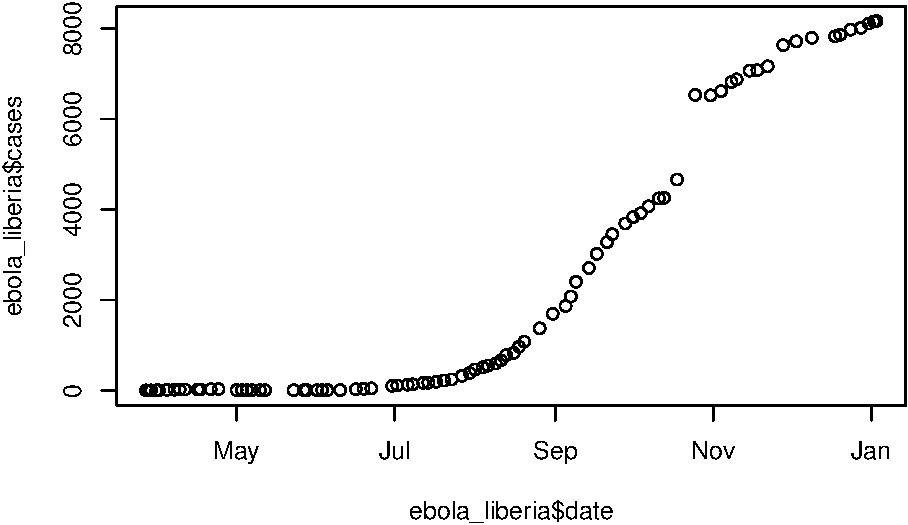
\includegraphics{RProgrammingForResearch_files/figure-latex/unnamed-chunk-127-1.pdf}

\subsection{A taste of what's to
come\ldots{}}\label{a-taste-of-whats-to-come}

Here's an example to give you a feel for why it's worth learning all
these different things about directories, \texttt{list.files}, and
pathnames.

The \texttt{measles\_data} subdirectory includes counts of measles made
at different times in different cities in California. Say that we wanted
to read them all in and make put them into one long dataframe with the
variables \texttt{city}, \texttt{count}, and \texttt{date}. You can put
together the things you've learned so far, along with a few new ideas
(including doing a loop), to do this very easily.

We'll talk more later about using loops and functions to make your
programming more efficient, but for right now just look through this
code and see if you can get a feel for how it's working (make sure your
directory for this course is your working directory):

\begin{Shaded}
\begin{Highlighting}[]
\NormalTok{## Create a vector of all the file names in the `measles_data` subdirectory}
\NormalTok{measles_files <-}\StringTok{ }\KeywordTok{list.files}\NormalTok{(}\StringTok{"data/measles_data"}\NormalTok{)}
\NormalTok{measles_files}
\end{Highlighting}
\end{Shaded}

\begin{verbatim}
##  [1] "02-09-2015.txt" "02-11-2015.txt" "02-13-2015.txt" "02-18-2015.txt"
##  [5] "02-20-2015.txt" "02-23-2015.txt" "02-25-2015.txt" "02-27-2015.txt"
##  [9] "03-02-2015.txt" "03-06-2015.txt" "03-13-2015.txt" "03-20-2015.txt"
## [13] "03-27-2015.txt" "04-03-2015.txt" "04-10-2015.txt" "04-17-2015.txt"
\end{verbatim}

\begin{Shaded}
\begin{Highlighting}[]
\NormalTok{## Create a vector of all the dates for files by taking the }
\NormalTok{## `.txt` off each of these file names and change it into}
\NormalTok{## a date}
\NormalTok{measles_dates <-}\StringTok{ }\KeywordTok{sub}\NormalTok{(}\StringTok{".txt"}\NormalTok{, }\StringTok{""}\NormalTok{, measles_files)}
\NormalTok{measles_dates}
\end{Highlighting}
\end{Shaded}

\begin{verbatim}
##  [1] "02-09-2015" "02-11-2015" "02-13-2015" "02-18-2015" "02-20-2015"
##  [6] "02-23-2015" "02-25-2015" "02-27-2015" "03-02-2015" "03-06-2015"
## [11] "03-13-2015" "03-20-2015" "03-27-2015" "04-03-2015" "04-10-2015"
## [16] "04-17-2015"
\end{verbatim}

\begin{Shaded}
\begin{Highlighting}[]
\KeywordTok{class}\NormalTok{(measles_dates)}
\end{Highlighting}
\end{Shaded}

\begin{verbatim}
## [1] "character"
\end{verbatim}

\begin{Shaded}
\begin{Highlighting}[]
\NormalTok{measles_dates <-}\StringTok{ }\KeywordTok{mdy}\NormalTok{(measles_dates)}
\NormalTok{measles_dates}
\end{Highlighting}
\end{Shaded}

\begin{verbatim}
##  [1] "2015-02-09" "2015-02-11" "2015-02-13" "2015-02-18" "2015-02-20"
##  [6] "2015-02-23" "2015-02-25" "2015-02-27" "2015-03-02" "2015-03-06"
## [11] "2015-03-13" "2015-03-20" "2015-03-27" "2015-04-03" "2015-04-10"
## [16] "2015-04-17"
\end{verbatim}

\begin{Shaded}
\begin{Highlighting}[]
\NormalTok{## Before I show the loop, let me talk you through some }
\NormalTok{## of the parts of it:}
\NormalTok{i <-}\StringTok{ }\DecValTok{1} \CommentTok{# I'm setting the index to 1}

\NormalTok{## Now I'll use `paste0` to create the first file name}
\NormalTok{## I want to read.}
\NormalTok{file_name <-}\StringTok{ }\KeywordTok{paste0}\NormalTok{(}\StringTok{"data/measles_data/"}\NormalTok{, measles_files[i])}
\NormalTok{file_name}
\end{Highlighting}
\end{Shaded}

\begin{verbatim}
## [1] "data/measles_data/02-09-2015.txt"
\end{verbatim}

\begin{Shaded}
\begin{Highlighting}[]
\NormalTok{## Now I'll read in that tab-delimited file}
\NormalTok{df <-}\StringTok{ }\KeywordTok{read_tsv}\NormalTok{(file_name, }\DataTypeTok{col_names =} \KeywordTok{c}\NormalTok{(}\StringTok{"city"}\NormalTok{, }\StringTok{"count"}\NormalTok{))}
\KeywordTok{head}\NormalTok{(df)}
\end{Highlighting}
\end{Shaded}

\begin{verbatim}
## # A tibble: 6 × 2
##                 city count
##                <chr> <int>
## 1            ALAMEDA     6
## 2        LOS ANGELES    20
## 3 City of Long Beach     2
## 4   City of Pasadena     4
## 5              MARIN     2
## 6             ORANGE    34
\end{verbatim}

\begin{Shaded}
\begin{Highlighting}[]
\NormalTok{## Now I'll add on a column with the date for all the }
\NormalTok{## values from that file. Notice that I'm using `i` to }
\NormalTok{## index this, as well}

\NormalTok{df <-}\StringTok{ }\KeywordTok{mutate}\NormalTok{(df, }\DataTypeTok{date =} \NormalTok{measles_dates[i])}
\KeywordTok{head}\NormalTok{(df)}
\end{Highlighting}
\end{Shaded}

\begin{verbatim}
## # A tibble: 6 × 3
##                 city count       date
##                <chr> <int>     <date>
## 1            ALAMEDA     6 2015-02-09
## 2        LOS ANGELES    20 2015-02-09
## 3 City of Long Beach     2 2015-02-09
## 4   City of Pasadena     4 2015-02-09
## 5              MARIN     2 2015-02-09
## 6             ORANGE    34 2015-02-09
\end{verbatim}

\begin{Shaded}
\begin{Highlighting}[]
\NormalTok{## Loop through and read in files. After the first file,}
\NormalTok{## add on the new information to the data that's already }
\NormalTok{## been read in. Note that you can use `rbind` to add on }
\NormalTok{## new rows to a dataframe as long as the new and old rows}
\NormalTok{## have the same number of columns and the same column names.}
\NormalTok{for(i in }\DecValTok{1}\NormalTok{:}\KeywordTok{length}\NormalTok{(measles_files))\{}
        \NormalTok{file_name <-}\StringTok{ }\KeywordTok{paste0}\NormalTok{(}\StringTok{"data/measles_data/"}\NormalTok{, measles_files[i])}
        \NormalTok{df <-}\StringTok{ }\KeywordTok{read.delim}\NormalTok{(file_name, }\DataTypeTok{header =} \OtherTok{FALSE}\NormalTok{, }
                         \DataTypeTok{col.names =} \KeywordTok{c}\NormalTok{(}\StringTok{"city"}\NormalTok{, }\StringTok{"count"}\NormalTok{))}
        \NormalTok{df <-}\StringTok{ }\KeywordTok{mutate}\NormalTok{(df, }\DataTypeTok{date =} \NormalTok{measles_dates[i])}
        \NormalTok{if(i ==}\StringTok{ }\DecValTok{1}\NormalTok{)\{}
                \NormalTok{ca_measles <-}\StringTok{ }\NormalTok{df}
        \NormalTok{\} else \{ }
                 \NormalTok{ca_measles <-}\StringTok{ }\KeywordTok{rbind}\NormalTok{(ca_measles, df)}
                \NormalTok{\}}
\NormalTok{\}}

\KeywordTok{dim}\NormalTok{(ca_measles)}
\end{Highlighting}
\end{Shaded}

\begin{verbatim}
## [1] 232   3
\end{verbatim}

\begin{Shaded}
\begin{Highlighting}[]
\KeywordTok{summary}\NormalTok{(ca_measles)}
\end{Highlighting}
\end{Shaded}

\begin{verbatim}
##                  city         count             date           
##  ALAMEDA           : 16   Min.   : 1.000   Min.   :2015-02-09  
##  City of Long Beach: 16   1st Qu.: 2.000   1st Qu.:2015-02-20  
##  City of Pasadena  : 16   Median : 4.000   Median :2015-03-02  
##  LOS ANGELES       : 16   Mean   : 8.698   Mean   :2015-03-07  
##  MARIN             : 16   3rd Qu.:12.000   3rd Qu.:2015-03-27  
##  ORANGE            : 16   Max.   :35.000   Max.   :2015-04-17  
##  (Other)           :136
\end{verbatim}

\begin{Shaded}
\begin{Highlighting}[]
\KeywordTok{library}\NormalTok{(ggplot2)}
\KeywordTok{ggplot}\NormalTok{(}\KeywordTok{subset}\NormalTok{(ca_measles, city %in%}\StringTok{ }\KeywordTok{c}\NormalTok{(}\StringTok{"LOS ANGELES"}\NormalTok{, }\StringTok{"SAN DIEGO"}\NormalTok{, }\StringTok{"ORANGE"}\NormalTok{)),}
       \KeywordTok{aes}\NormalTok{(}\DataTypeTok{x =} \NormalTok{date, }\DataTypeTok{y =} \NormalTok{count)) +}\StringTok{ }
\StringTok{        }\KeywordTok{geom_line}\NormalTok{()  +}\StringTok{ }
\StringTok{        }\KeywordTok{facet_grid}\NormalTok{(. ~}\StringTok{ }\NormalTok{city)}
\end{Highlighting}
\end{Shaded}

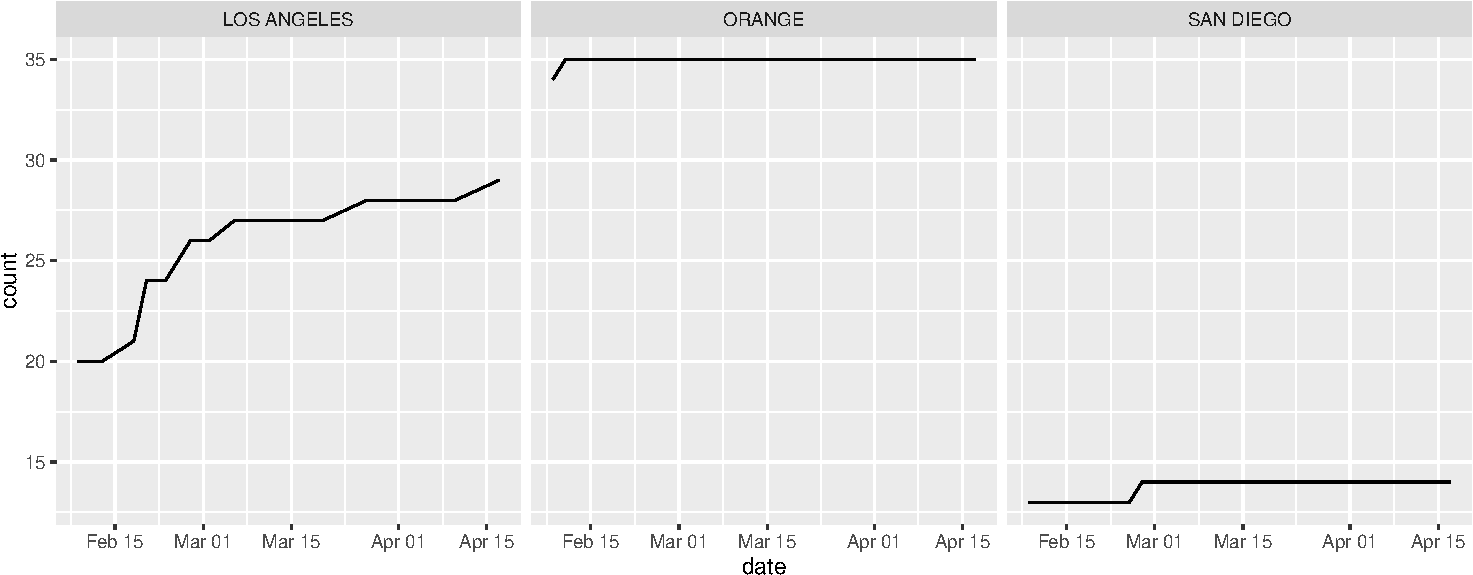
\includegraphics{RProgrammingForResearch_files/figure-latex/unnamed-chunk-128-1.pdf}

\chapter{Exploring data \#1}\label{exploring-data-1}

\href{https://github.com/geanders/RProgrammingForResearch/raw/master/slides/CourseNotes_Week3.pdf}{Download}
a pdf of the lecture slides covering this topic.

\section{Data from a package}\label{data-from-a-package}

So far we've covered three ways to get data into R:

\begin{enumerate}
\def\labelenumi{\arabic{enumi}.}
\tightlist
\item
  From flat files (either on your computer or online)
\item
  From files like SAS and Excel
\item
  From R objects (i.e., using \texttt{load()})
\end{enumerate}

Many R packages come with their own data, which is very easy to load and
use. For example, the \texttt{faraway} package, which complements Julian
Faraway's book \emph{Linear Models with R} (available as an ebook from
the CSU library), has a dataset called \texttt{worldcup} that I'll use
for some examples and that you'll use for part of this week's in-course
exercise. To load this dataset, first load the package with the data
(\texttt{faraway}) and then use the \texttt{data()} function with the
dataset name (``worldcup'') as the argument to the \texttt{data}
function:

\begin{Shaded}
\begin{Highlighting}[]
\KeywordTok{library}\NormalTok{(faraway)}
\KeywordTok{data}\NormalTok{(}\StringTok{"worldcup"}\NormalTok{)}
\end{Highlighting}
\end{Shaded}

Unlike most data objects you'll work with, datasets that are part of an
R package will often have their own help files. You can access this help
file for a dataset using the \texttt{?} operator with the dataset's
name:

\begin{Shaded}
\begin{Highlighting}[]
\NormalTok{?worldcup}
\end{Highlighting}
\end{Shaded}

This helpful will usually include information about the size of the
dataset, as well as definitions for each of the columns.

To get a list of all of the datasets that are available in the packages
you currently have loaded, run \texttt{data()} without an option inside
the parentheses:

\begin{Shaded}
\begin{Highlighting}[]
\KeywordTok{data}\NormalTok{()}
\end{Highlighting}
\end{Shaded}

\begin{rmdnote}
If you run the \texttt{library} function without any arguments
(\texttt{library()}), it works in a similar way-- R will open a list of
all the R packages that you have installed on your computer and can open
with a \texttt{library} call.
\end{rmdnote}

\section{Plots to explore data}\label{plots-to-explore-data}

Exploratory data analysis is a key step in data analysis, and plotting
your data in different ways is an important part of this process. In
this section, I will focus on the basics of \texttt{ggplot2} plotting,
to get you started creating some plots to explore your data. This
section will focus on making \textbf{useful}, rather than
\textbf{attractive} graphs, since at this stage we are focusing on
exploring data for yourself rather than presenting results to others.
Next week, I will explain more about how you can customize ggplot
objects, to help you make plots to communicate with others.

All of the plots we'll make today will use the \texttt{ggplot2} package
(another member of the tidyverse!). If you don't already have that
installed, you'll need to install it. You then need to load the package
in your current session of R:

\begin{Shaded}
\begin{Highlighting}[]
\CommentTok{# install.packages("ggplot2")  ## Uncomment and run if you don't have `ggplot2` installed}
\KeywordTok{library}\NormalTok{(ggplot2)}
\end{Highlighting}
\end{Shaded}

The process of creating a plot using \texttt{ggplot2} follows
conventions that are a bit different than most of the code you've seen
so far in R (although it is somewhat similar to the idea of piping I
introduced in the last chapter). The basic steps behind creating a plot
with \texttt{ggplot2} are:

\begin{enumerate}
\def\labelenumi{\arabic{enumi}.}
\tightlist
\item
  Create an object of the \texttt{ggplot} class, typically specifying
  the \textbf{data} and some or all of the \textbf{aesthetics};
\item
  Add on \textbf{geoms} and other elements to create and customize the
  plot, using \texttt{+}.
\end{enumerate}

You can add on one or many geoms and other elements to create plots that
range from very simple to very customized. This week, we'll focus on
simple geoms and added elements, and then explore more detailed
customization next week.

\begin{rmdwarning}
If R gets to the end of a line and there is not some indication that the
call is not over (e.g., \texttt{\%\textgreater{}\%} for piping or
\texttt{+} for \texttt{ggplot2} plots), R interprets that as a message
to run the call without reading in further code. A common error when
writing \texttt{ggplot2} code is to put the \texttt{+} to add a geom or
element at the beginning of a line rather than the end of a previous
line-- in this case, R will try to execute the call too soon. To avoid
errors, be sure to end lines with \texttt{+}, don't start lines with it.
\end{rmdwarning}

\subsection{Initializing a ggplot
object}\label{initializing-a-ggplot-object}

The first step in creating a plot using \texttt{ggplot2} is to create a
ggplot object. This object will not, by itself, create a plot with
anything in it. Instead, it typically specifies the data frame you want
to use and which aesthetics will be mapped to certain columns of that
data frame (aesthetics are explained more in the next subsection).

Use the following conventions to initialize a ggplot object:

\begin{Shaded}
\begin{Highlighting}[]
\NormalTok{## Generic code}
\NormalTok{object <-}\StringTok{ }\KeywordTok{ggplot}\NormalTok{(dataframe, }\KeywordTok{aes}\NormalTok{(}\DataTypeTok{x =} \NormalTok{column_1, }\DataTypeTok{y =} \NormalTok{column_2))}
\end{Highlighting}
\end{Shaded}

The data frame is the first parameter in a \texttt{ggplot} call and, if
you like, you can use the parameter definition with that call (e.g.,
\texttt{data\ =\ dataframe}). Aesthetics are defined within an
\texttt{aes} function call that typically is used within the
\texttt{ggplot} call.

\begin{rmdnote}
While the \texttt{ggplot} call is the place where you will most often
see an \texttt{aes} call, \texttt{aes} can also be used within the calls
to add specific geoms. This can be particularly useful if you want to
map aesthetics differently for different geoms in your plot. We'll see
some examples of this use of \texttt{aes} more in later sections, when
we talk about customizing plots. The \texttt{data} parameter can also be
used in geom calls, to use a different data frame from the one defined
when creating the original ggplot object, although this tends to be less
common.
\end{rmdnote}

\subsection{Plot aesthetics}\label{plot-aesthetics}

\textbf{Aesthetics} are properties of the plot that can show certain
elements of the data. For example, in Figure \ref{fig:aesmapex}, color
shows (is mapped to) gender, x-position shows height, and y-position
shows weight in a sample data set of measurements of children in Nepal.

\begin{figure}

{\centering 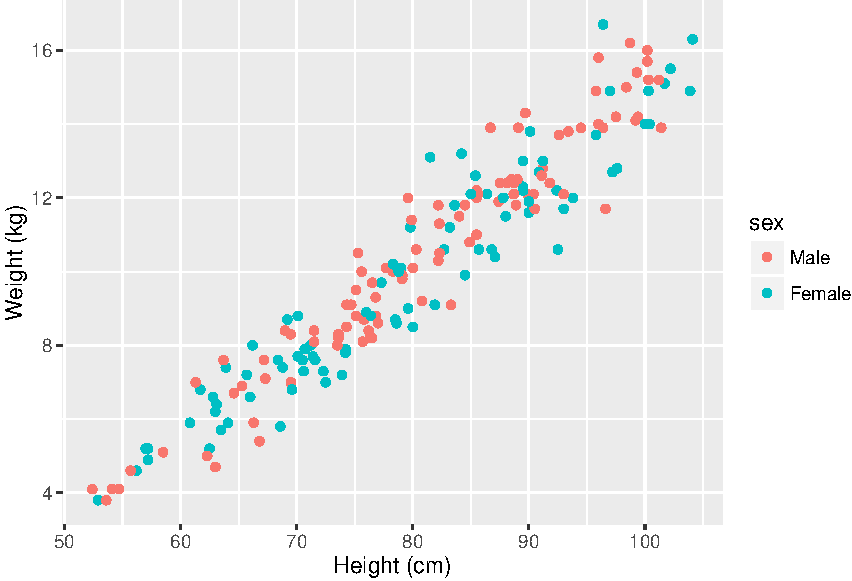
\includegraphics{RProgrammingForResearch_files/figure-latex/aesmapex-1} 

}

\caption{Example of how different properties of a plot can show different elements to the data. Here, color indicates gender, position along the x-axis shows height, and position along the y-axis shows weight. This example is a subset of data from the `nepali` dataset in the `faraway` package.}\label{fig:aesmapex}
\end{figure}

\begin{rmdnote}
Any of these aesthetics could also be given a constant value, instead of
being mapped to an element of the data. For example, all the points
could be red, instead of showing gender.
\end{rmdnote}

Which aesthetics are required for a plot depend on which geoms (more on
those in a second) you're adding to the plot. You can find out the
aesthetics you can use for a geom in the ``Aesthetics'' section of the
geom's help file (e.g., \texttt{?geom\_point}). Required aesthetics are
in bold in this section of the help file and optional ones are not.
Common plot aesthetics you might want to specify include:

\begin{tabular}{l|l}
\hline
Code & Description\\
\hline
`x` & Position on x-axis\\
\hline
`y` & Position on y-axis\\
\hline
`shape` & Shape\\
\hline
`color` & Color of border of elements\\
\hline
`fill` & Color of inside of elements\\
\hline
`size` & Size\\
\hline
`alpha` & Transparency (1: opaque; 0: transparent)\\
\hline
`linetype` & Type of line (e.g., solid, dashed)\\
\hline
\end{tabular}

\subsection{Adding geoms}\label{adding-geoms}

Next, you'll want to add one or more \texttt{geoms} to create the plot.
You can add these with \texttt{+} after the \texttt{ggplot} statement to
initialize the ggplot object. Some of the most common geoms are:

\begin{tabular}{l|l}
\hline
Plot type & ggplot2 function\\
\hline
Histogram (1 numeric variable) & `geom\_histogram`\\
\hline
Scatterplot (2 numeric variables) & `geom\_point`\\
\hline
Boxplot (1 numeric variable, possibly 1 factor variable) & `geom\_boxplot`\\
\hline
Line graph (2 numeric variables) & `geom\_line`\\
\hline
\end{tabular}

\subsection{Constant aesthetics}\label{constant-aesthetics}

Instead of mapping an aesthetic to an element of your data, you can use
a constant value for it. For example, you may want to make all the
points green, rather than having color map to gender:

\begin{center}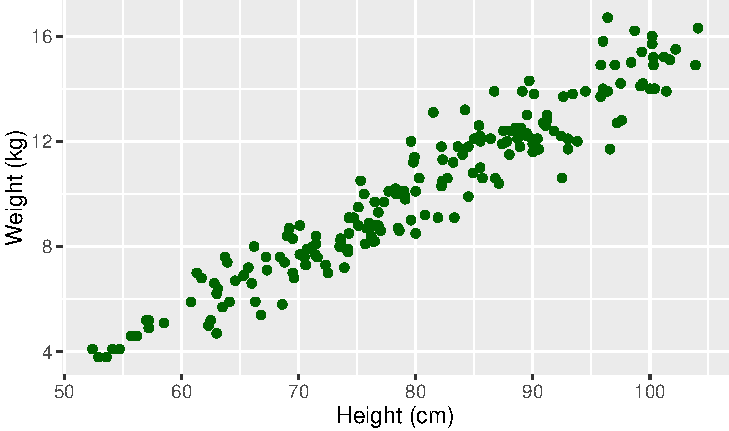
\includegraphics[width=0.6\textwidth]{RProgrammingForResearch_files/figure-latex/unnamed-chunk-140-1} \end{center}

In this case, you'll define that aesthetic when you add the geom,
outside of an \texttt{aes} statement. In R, you can specify the shape of
points with a number. Figure \ref{fig:shapeexamples} shows the shapes
that correspond to the numbers 1 to 25 in the \texttt{shape} aesthetic.
This figure also provides an example of the difference between color
(black for all these example points) and fill (red for these examples).
You can see that some point shapes include a fill (21 for example),
while some are either empty (1) or solid (19).

\begin{figure}

{\centering 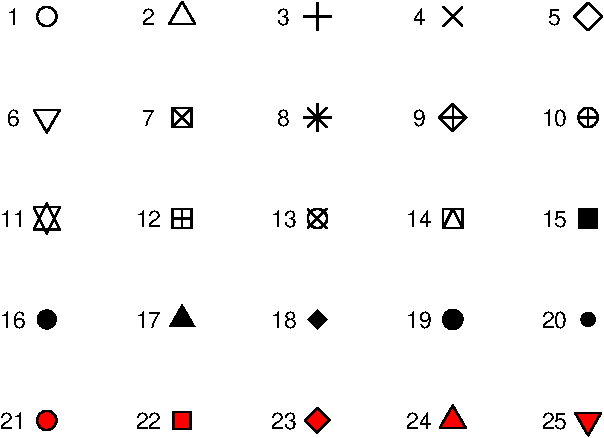
\includegraphics{RProgrammingForResearch_files/figure-latex/shapeexamples-1} 

}

\caption{Examples of the shapes corresponding to different numeric choices for the `shape` aesthetic. For all examples, `color` is set to black and `fill` to red.}\label{fig:shapeexamples}
\end{figure}

If you want to set color to be a constant value, you can do that in R
using character strings for different colors. Figure
\ref{fig:colorexamples} gives an example of some of the different blues
available in R. To find links to listings of different R colors, google
``R colors'' and search by ``Images''.

\begin{figure}

{\centering 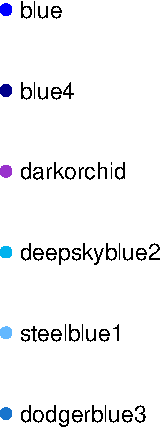
\includegraphics{RProgrammingForResearch_files/figure-latex/colorexamples-1} 

}

\caption{Example of available shades of blue in R.}\label{fig:colorexamples}
\end{figure}

\subsection{Useful plot additions}\label{useful-plot-additions}

There are also a number of elements that you can add onto a
\texttt{ggplot} object using \texttt{+}. A few that are used very
frequently are:

\begin{tabular}{l|l}
\hline
Element & Description\\
\hline
`ggtitle` & Plot title\\
\hline
`xlab`, `ylab` & x- and y-axis labels\\
\hline
`xlim`, `ylim` & Limits of x- and y-axis\\
\hline
\end{tabular}

\subsection{Example dataset}\label{example-dataset}

For the example plots, I'll use a dataset in the \texttt{faraway}
package called \texttt{nepali}. This gives data from a study of the
health of a group of Nepalese children.

\begin{Shaded}
\begin{Highlighting}[]
\KeywordTok{library}\NormalTok{(faraway)}
\KeywordTok{data}\NormalTok{(nepali)}
\end{Highlighting}
\end{Shaded}

I'll be using functions from \texttt{dplyr} and \texttt{ggplot2}, so
those need to be loaded:

\begin{Shaded}
\begin{Highlighting}[]
\KeywordTok{library}\NormalTok{(dplyr)}
\KeywordTok{library}\NormalTok{(ggplot2)}
\end{Highlighting}
\end{Shaded}

Each observation is a single measurement for a child; there can be
multiple observations per child. I used the following code to select
only the columns for child id, sex, weight, height, and age. I also used
\texttt{distinct} to limit the dataset to only include one measurement
for each chile, the child's first measurement in the dataset.

\begin{Shaded}
\begin{Highlighting}[]
\NormalTok{nepali <-}\StringTok{ }\NormalTok{nepali %>%}
\StringTok{  }\KeywordTok{select}\NormalTok{(id, sex, wt, ht, age) %>%}
\StringTok{  }\KeywordTok{mutate}\NormalTok{(}\DataTypeTok{id =} \KeywordTok{factor}\NormalTok{(id),}
         \DataTypeTok{sex =} \KeywordTok{factor}\NormalTok{(sex, }\DataTypeTok{levels =} \KeywordTok{c}\NormalTok{(}\DecValTok{1}\NormalTok{, }\DecValTok{2}\NormalTok{),}
                      \DataTypeTok{labels =} \KeywordTok{c}\NormalTok{(}\StringTok{"Male"}\NormalTok{, }\StringTok{"Female"}\NormalTok{))) %>%}
\StringTok{  }\KeywordTok{distinct}\NormalTok{(id, }\DataTypeTok{.keep_all =} \OtherTok{TRUE}\NormalTok{)}
\end{Highlighting}
\end{Shaded}

After this cleaning, the data looks like this:

\begin{Shaded}
\begin{Highlighting}[]
\KeywordTok{head}\NormalTok{(nepali)}
\end{Highlighting}
\end{Shaded}

\begin{verbatim}
##       id    sex   wt    ht age
## 1 120011   Male 12.8  91.2  41
## 2 120012 Female 14.9 103.9  57
## 3 120021 Female  7.7  70.1   8
## 4 120022 Female 12.1  86.4  35
## 5 120023   Male 14.2  99.4  49
## 6 120031   Male 13.9  96.4  46
\end{verbatim}

\subsection{Histograms}\label{histograms}

Histograms show the distribution of a single variable. Therefore,
\texttt{geom\_histogram()} requires only one main aesthetic, \texttt{x},
the (numeric) vector for which you want to create a histogram. For
example, to create a histogram of children's heights for the Nepali
dataset (Figure \ref{fig:nepalihist1}), run:

\begin{Shaded}
\begin{Highlighting}[]
\KeywordTok{ggplot}\NormalTok{(nepali, }\KeywordTok{aes}\NormalTok{(}\DataTypeTok{x =} \NormalTok{ht)) +}\StringTok{ }
\StringTok{  }\KeywordTok{geom_histogram}\NormalTok{()}
\end{Highlighting}
\end{Shaded}

\begin{figure}

{\centering 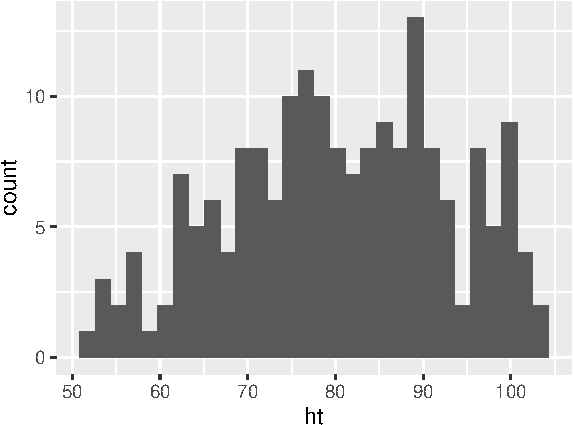
\includegraphics{RProgrammingForResearch_files/figure-latex/nepalihist1-1} 

}

\caption{Basic example of plotting a histogram with `ggplot2`. This histogram shows the distribution of heights for the first recorded measurements of each child in the `nepali` dataset.}\label{fig:nepalihist1}
\end{figure}

\begin{rmdnote}
If you run the code with no arguments for \texttt{binwidth} or
\texttt{bins} in \texttt{geom\_histogram}, you will get a message saying
``\texttt{stat\_bin()} using \texttt{bins\ =\ 30}. Pick better value
with \texttt{binwidth}.''. This message is just saying that a default
number of bins was used to create the histogram. You can use arguments
to change the number of bins used, but often this default is fine. You
may also get a message that observations with missing values were
removed.
\end{rmdnote}

You can add some elements to the histogram now to customize it a bit.
For example (Figure @ref()), you can add a figure title
(\texttt{ggtitle}) and clearer labels for the x-axis (\texttt{xlab}).
You can also change the range of values shown by the x-axis
(\texttt{xlim}).

\begin{Shaded}
\begin{Highlighting}[]
\KeywordTok{ggplot}\NormalTok{(nepali, }\KeywordTok{aes}\NormalTok{(}\DataTypeTok{x =} \NormalTok{ht)) +}\StringTok{ }
\StringTok{  }\KeywordTok{geom_histogram}\NormalTok{(}\DataTypeTok{fill =} \StringTok{"lightblue"}\NormalTok{, }\DataTypeTok{color =} \StringTok{"black"}\NormalTok{) +}\StringTok{ }
\StringTok{  }\KeywordTok{ggtitle}\NormalTok{(}\StringTok{"Height of children"}\NormalTok{) +}\StringTok{ }
\StringTok{  }\KeywordTok{xlab}\NormalTok{(}\StringTok{"Height (cm)"}\NormalTok{) +}\StringTok{ }\KeywordTok{xlim}\NormalTok{(}\KeywordTok{c}\NormalTok{(}\DecValTok{0}\NormalTok{, }\DecValTok{120}\NormalTok{))}
\end{Highlighting}
\end{Shaded}

\begin{figure}

{\centering 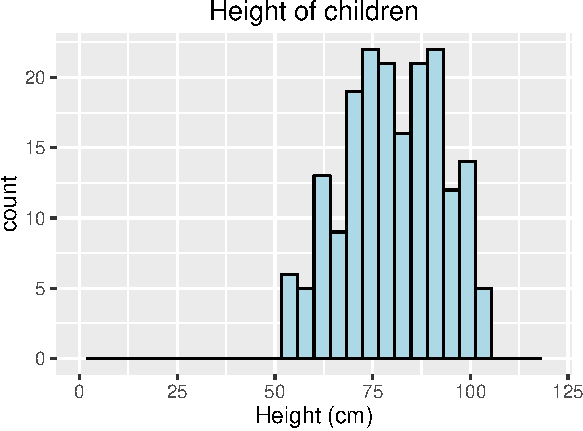
\includegraphics{RProgrammingForResearch_files/figure-latex/nepalihist2-1} 

}

\caption{Example of adding ggplot elements to customize a histogram.}\label{fig:nepalihist2}
\end{figure}

The geom \texttt{geom\_histogram} also has special argument for setting
the number of width of the bins used in the histogram. Figure \ref{fig}
shows an example of how you can use the \texttt{bins} argument to change
the number of bins that are used to make the histogram of height for the
\texttt{nepali} dataset.

\begin{Shaded}
\begin{Highlighting}[]
\KeywordTok{ggplot}\NormalTok{(nepali, }\KeywordTok{aes}\NormalTok{(}\DataTypeTok{x =} \NormalTok{ht)) +}\StringTok{ }
\StringTok{  }\KeywordTok{geom_histogram}\NormalTok{(}\DataTypeTok{fill =} \StringTok{"lightblue"}\NormalTok{, }\DataTypeTok{color =} \StringTok{"black"}\NormalTok{,}
                 \DataTypeTok{bins =} \DecValTok{40}\NormalTok{) }
\end{Highlighting}
\end{Shaded}

\begin{figure}

{\centering 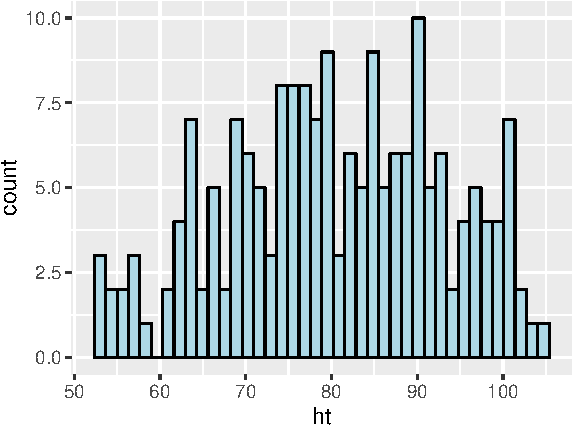
\includegraphics{RProgrammingForResearch_files/figure-latex/nepalihist3-1} 

}

\caption{Example of using the `bins` argument to change the number of bins used in a histogram.}\label{fig:nepalihist3}
\end{figure}

Similarly, the \texttt{binwidth} argument can be used to set the width
of bins. Figure \ref{fig:nepalihist4} shows an example of using this
function to create a histogram of the Nepali children's heights with
binwidths of 10 centimeters (note that this argument is set in the same
units as the x variable).

\begin{Shaded}
\begin{Highlighting}[]
\KeywordTok{ggplot}\NormalTok{(nepali, }\KeywordTok{aes}\NormalTok{(}\DataTypeTok{x =} \NormalTok{ht)) +}\StringTok{ }
\StringTok{  }\KeywordTok{geom_histogram}\NormalTok{(}\DataTypeTok{fill =} \StringTok{"lightblue"}\NormalTok{, }\DataTypeTok{color =} \StringTok{"black"}\NormalTok{,}
                 \DataTypeTok{binwidth =} \DecValTok{10}\NormalTok{) }
\end{Highlighting}
\end{Shaded}

\begin{figure}

{\centering 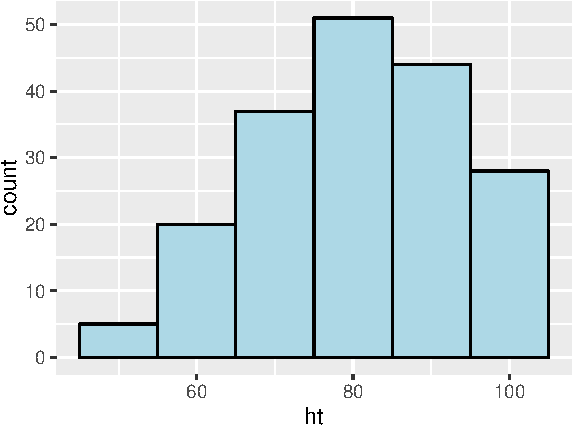
\includegraphics{RProgrammingForResearch_files/figure-latex/nepalihist4-1} 

}

\caption{Example of using the `binwidth` argument to set the width of each bin used in a histogram.}\label{fig:nepalihist4}
\end{figure}

\subsection{Scatterplots}\label{scatterplots}

A scatterplot shows how one variable changes as another changes. You can
use the \texttt{geom\_point} geom to create a scatterplot. For example,
to create a scatterplot of height versus age for the Nepali data (Figure
\ref{fig:nepaliscatter1}), you can run the following code:

\begin{Shaded}
\begin{Highlighting}[]
\KeywordTok{ggplot}\NormalTok{(nepali, }\KeywordTok{aes}\NormalTok{(}\DataTypeTok{x =} \NormalTok{ht, }\DataTypeTok{y =} \NormalTok{wt)) +}\StringTok{ }
\StringTok{  }\KeywordTok{geom_point}\NormalTok{()}
\end{Highlighting}
\end{Shaded}

\begin{figure}

{\centering 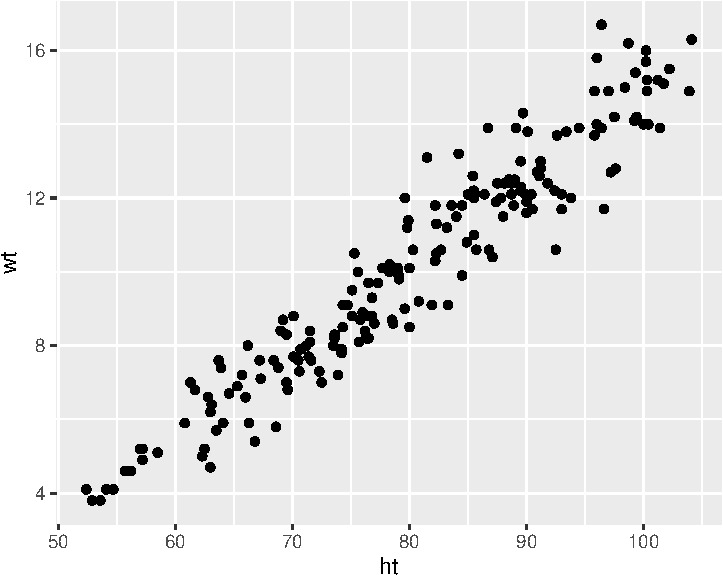
\includegraphics{RProgrammingForResearch_files/figure-latex/nepaliscatter1-1} 

}

\caption{Example of creating a scatterplot. This scatterplot shows the relationship between children's heights and weights within the nepali dataset.}\label{fig:nepaliscatter1}
\end{figure}

Again, you can use some of the options and additions to change the plot
appearance. For example, to add a title, change the x- and y-axis
labels, and change the color and size of the points on the scatterplot
(Figure \ref{fig:nepaliscatter2}), you can run:

\begin{Shaded}
\begin{Highlighting}[]
\KeywordTok{ggplot}\NormalTok{(nepali, }\KeywordTok{aes}\NormalTok{(}\DataTypeTok{x =} \NormalTok{ht, }\DataTypeTok{y =} \NormalTok{wt)) +}\StringTok{ }
\StringTok{  }\KeywordTok{geom_point}\NormalTok{(}\DataTypeTok{color =} \StringTok{"blue"}\NormalTok{, }\DataTypeTok{size =} \FloatTok{0.5}\NormalTok{) +}\StringTok{ }
\StringTok{  }\KeywordTok{ggtitle}\NormalTok{(}\StringTok{"Weight versus Height"}\NormalTok{) +}\StringTok{ }
\StringTok{  }\KeywordTok{xlab}\NormalTok{(}\StringTok{"Height (cm)"}\NormalTok{) +}\StringTok{ }\KeywordTok{ylab}\NormalTok{(}\StringTok{"Weight (kg)"}\NormalTok{)}
\end{Highlighting}
\end{Shaded}

\begin{figure}

{\centering 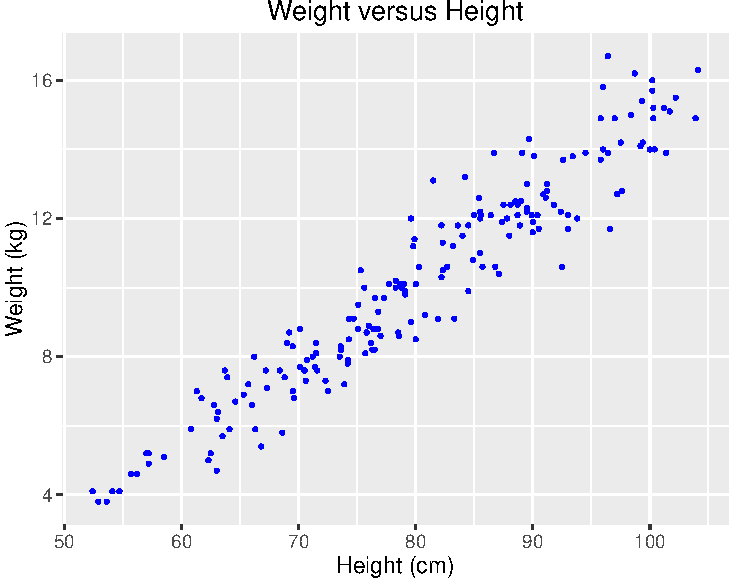
\includegraphics{RProgrammingForResearch_files/figure-latex/nepaliscatter2-1} 

}

\caption{Example of adding ggplot elements to customize a scatterplot.}\label{fig:nepaliscatter2}
\end{figure}

You can also try mapping another variable in the dataset to the
\texttt{color} aesthetic. For example, to use color to show the sex of
each child in the scatterplot (Figure \ref{fig:nepaliscatter3}), you can
run:

\begin{Shaded}
\begin{Highlighting}[]
\KeywordTok{ggplot}\NormalTok{(nepali, }\KeywordTok{aes}\NormalTok{(}\DataTypeTok{x =} \NormalTok{ht, }\DataTypeTok{y =} \NormalTok{wt, }\DataTypeTok{color =} \NormalTok{sex)) +}\StringTok{ }
\StringTok{  }\KeywordTok{geom_point}\NormalTok{(}\DataTypeTok{size =} \FloatTok{0.5}\NormalTok{) +}\StringTok{ }
\StringTok{  }\KeywordTok{ggtitle}\NormalTok{(}\StringTok{"Weight versus Height"}\NormalTok{) +}\StringTok{ }
\StringTok{  }\KeywordTok{xlab}\NormalTok{(}\StringTok{"Height (cm)"}\NormalTok{) +}\StringTok{ }\KeywordTok{ylab}\NormalTok{(}\StringTok{"Weight (kg)"}\NormalTok{)}
\end{Highlighting}
\end{Shaded}

\begin{figure}

{\centering 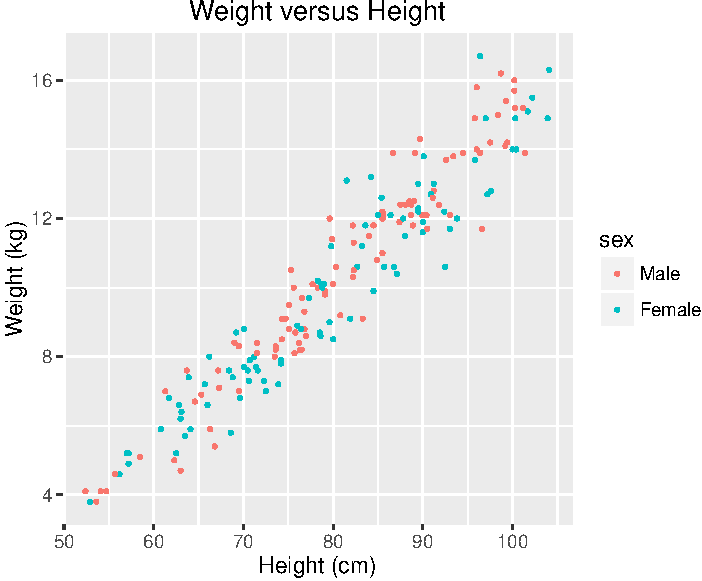
\includegraphics{RProgrammingForResearch_files/figure-latex/nepaliscatter3-1} 

}

\caption{Example of mapping color to an element of the data in a scatterplot.}\label{fig:nepaliscatter3}
\end{figure}

\subsection{Boxplots}\label{boxplots}

Boxplots can be used to show the distribution of a continuous variable.
To create a boxplot, you can use the \texttt{geom\_boxplot} geom. To
plot a boxplot for a single, continuous variable, you can map that
variable to \texttt{y} in the \texttt{aes} call, and map \texttt{x} to
the constant \texttt{1}. For example, to create a boxplot of the heights
of children in the Nepali dataset (Figure \ref{fig:nepaliboxplot1}), you
can run:

\begin{Shaded}
\begin{Highlighting}[]
\KeywordTok{ggplot}\NormalTok{(nepali, }\KeywordTok{aes}\NormalTok{(}\DataTypeTok{x =} \DecValTok{1}\NormalTok{, }\DataTypeTok{y =} \NormalTok{ht)) +}\StringTok{ }
\StringTok{  }\KeywordTok{geom_boxplot}\NormalTok{() +}\StringTok{ }
\StringTok{  }\KeywordTok{xlab}\NormalTok{(}\StringTok{""}\NormalTok{)+}\StringTok{ }\KeywordTok{ylab}\NormalTok{(}\StringTok{"Height (cm)"}\NormalTok{)}
\end{Highlighting}
\end{Shaded}

\begin{figure}

{\centering 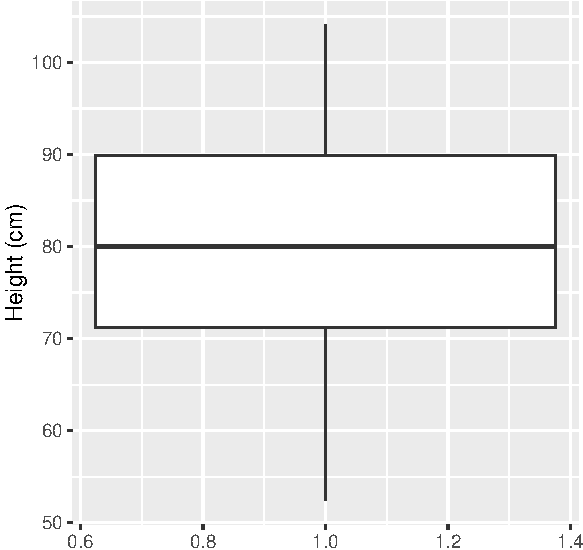
\includegraphics{RProgrammingForResearch_files/figure-latex/nepaliboxplot1-1} 

}

\caption{Example of creating a boxplot. The example shows the distribution of height data for children in the nepali dataset.}\label{fig:nepaliboxplot1}
\end{figure}

You can also create separate boxplots, one for each level of a factor
(Figure \ref{fig:nepaliboxplot2}). In this case, you'll need to include
two aesthetics (\texttt{x} and \texttt{y}) when you initialize the
ggplot object The \texttt{y} variable is the variable for which the
distribution will be shown, and the \texttt{x} variable should be a
discrete (categorical or TRUE/FALSE) variable, and will be used to group
the variable. This \texttt{x} variable should also be specified as the
grouping variable, using \texttt{group} within the aesthetic call.

\begin{Shaded}
\begin{Highlighting}[]
\KeywordTok{ggplot}\NormalTok{(nepali, }\KeywordTok{aes}\NormalTok{(}\DataTypeTok{x =} \NormalTok{sex, }\DataTypeTok{y =} \NormalTok{ht, }\DataTypeTok{group =} \NormalTok{sex)) +}\StringTok{ }
\StringTok{  }\KeywordTok{geom_boxplot}\NormalTok{() +}\StringTok{ }
\StringTok{  }\KeywordTok{xlab}\NormalTok{(}\StringTok{"Sex"}\NormalTok{)+}\StringTok{ }\KeywordTok{ylab}\NormalTok{(}\StringTok{"Height (cm)"}\NormalTok{) }
\end{Highlighting}
\end{Shaded}

\begin{figure}

{\centering 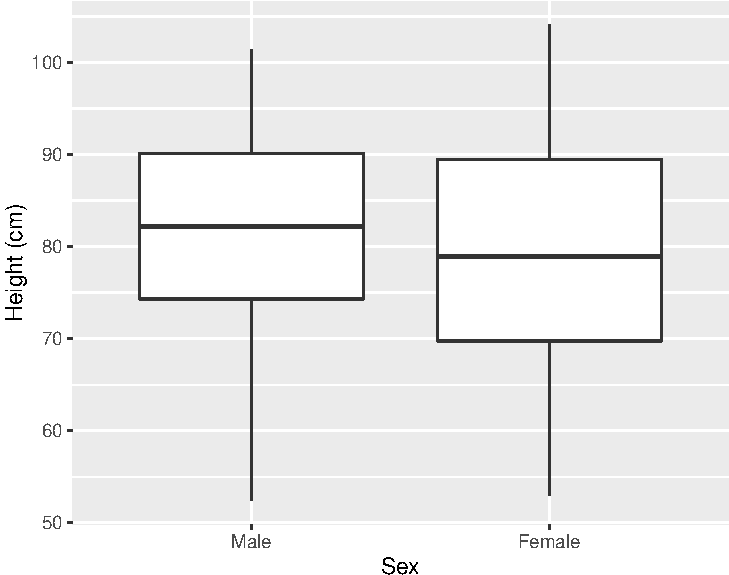
\includegraphics{RProgrammingForResearch_files/figure-latex/nepaliboxplot2-1} 

}

\caption{Example of creating separate boxplots, divided by a categorical grouping variable in the data.}\label{fig:nepaliboxplot2}
\end{figure}

\subsection{\texorpdfstring{Extensions of
\texttt{ggplot2}}{Extensions of ggplot2}}\label{extensions-of-ggplot2}

There are lots of R extensions for creating other interesting plots. For
example, you can use the \texttt{ggpairs} function from the
\texttt{GGally} package to plot all pairs of scatterplots for several
variables (Figure \ref{fig:ggallyexample}).

\begin{Shaded}
\begin{Highlighting}[]
\KeywordTok{library}\NormalTok{(GGally)}
\KeywordTok{ggpairs}\NormalTok{(nepali %>%}\StringTok{ }\KeywordTok{select}\NormalTok{(sex, wt, ht, age))}
\end{Highlighting}
\end{Shaded}

\begin{figure}

{\centering 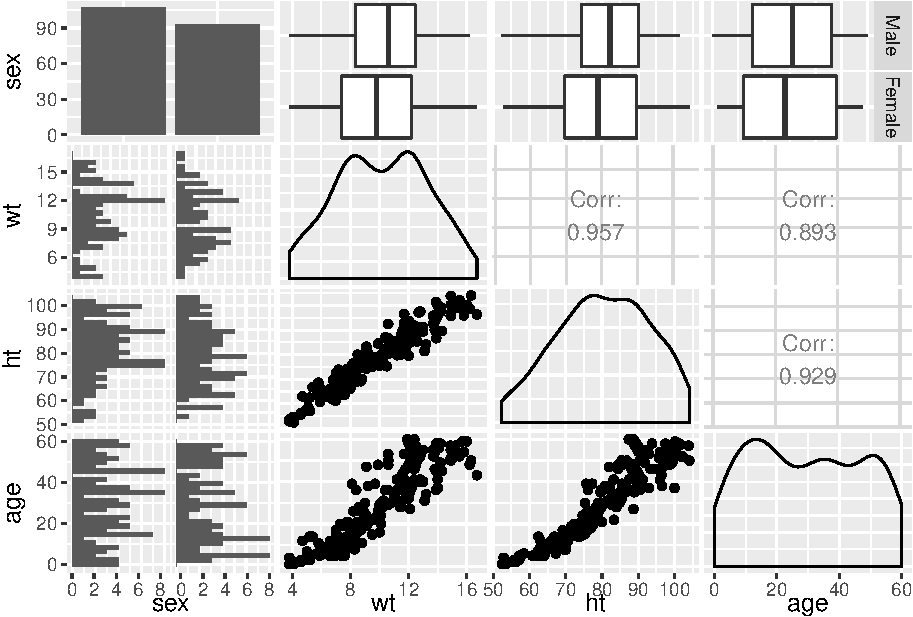
\includegraphics[width=\textwidth]{RProgrammingForResearch_files/figure-latex/ggallyexample-1} 

}

\caption{Example of using ggpairs from the GGally package for exploratory data analysis.}\label{fig:ggallyexample}
\end{figure}

Notice how this output shows continuous and binary variables
differently. For example, the center diagonal shows density plots for
continuous variables, but a bar chart for the categorical variable.

See \url{https://www.ggplot2-exts.org} to find more \texttt{ggplot2}
extensions.

\section{Simple statistics functions}\label{simple-statistics-functions}

\subsection{Summary statistics}\label{summary-statistics}

To explore your data, you'll need to be able to calculate some simple
statistics for vectors, including calculating the mean and range of
continuous variables and counting the number of values in each category
of a factor or logical vector.

Here are some simple statistics functions you will likely use often:

\begin{longtable}[c]{@{}ll@{}}
\toprule
Function & Description\tabularnewline
\midrule
\endhead
\texttt{range()} & Range (minimum and maximum) of vector\tabularnewline
\texttt{min()}, \texttt{max()} & Minimum or maximum of
vector\tabularnewline
\texttt{mean()}, \texttt{median()} & Mean or median of
vector\tabularnewline
\texttt{sd()} & Standard deviation of vector\tabularnewline
\texttt{table()} & Number of observations per level for a factor
vector\tabularnewline
\texttt{cor()} & Determine correlation(s) between two or more
vectors\tabularnewline
\texttt{summary()} & Summary statistics, depends on class\tabularnewline
\bottomrule
\end{longtable}

All of these functions take, as the main argument, the vector or vectors
for which you want the statistic. If there are missing values in the
vector, you'll typically need to add an argument to say what to do with
the missing values. The parameter name for this varies by function, but
for many of these functions it's \texttt{na.rm\ =\ TRUE} or
\texttt{use="complete.obs"}.

\begin{Shaded}
\begin{Highlighting}[]
\KeywordTok{mean}\NormalTok{(nepali$wt, }\DataTypeTok{na.rm =} \OtherTok{TRUE}\NormalTok{)}
\end{Highlighting}
\end{Shaded}

\begin{verbatim}
## [1] 10.18432
\end{verbatim}

\begin{Shaded}
\begin{Highlighting}[]
\KeywordTok{range}\NormalTok{(nepali$ht, }\DataTypeTok{na.rm =} \OtherTok{TRUE}\NormalTok{)}
\end{Highlighting}
\end{Shaded}

\begin{verbatim}
## [1]  52.4 104.1
\end{verbatim}

\begin{Shaded}
\begin{Highlighting}[]
\KeywordTok{sd}\NormalTok{(nepali$ht, }\DataTypeTok{na.rm =} \OtherTok{TRUE}\NormalTok{)}
\end{Highlighting}
\end{Shaded}

\begin{verbatim}
## [1] 12.64529
\end{verbatim}

\begin{Shaded}
\begin{Highlighting}[]
\KeywordTok{table}\NormalTok{(nepali$sex)}
\end{Highlighting}
\end{Shaded}

\begin{verbatim}
## 
##   Male Female 
##    107     93
\end{verbatim}

Most of these functions take a single vector as the input. The
\texttt{cor} function, however, calculates the correlation between
vectors and so takes two or more vectors. If you give it multiple
values, it will give the correlation matrix for all the vectors.

\begin{Shaded}
\begin{Highlighting}[]
\KeywordTok{cor}\NormalTok{(nepali$wt, nepali$ht, }\DataTypeTok{use =} \StringTok{"complete.obs"}\NormalTok{)}
\end{Highlighting}
\end{Shaded}

\begin{verbatim}
## [1] 0.9571535
\end{verbatim}

\begin{Shaded}
\begin{Highlighting}[]
\KeywordTok{cor}\NormalTok{((nepali %>%}\StringTok{ }\KeywordTok{select}\NormalTok{(wt, ht, age)), }\DataTypeTok{use =} \StringTok{"complete.obs"}\NormalTok{)}
\end{Highlighting}
\end{Shaded}

\begin{verbatim}
##            wt        ht       age
## wt  1.0000000 0.9571535 0.8931195
## ht  0.9571535 1.0000000 0.9287129
## age 0.8931195 0.9287129 1.0000000
\end{verbatim}

R supports object-oriented programming. Your first taste of this shows
up with the \texttt{summary} function. For the \texttt{summary}
function, R does not run the same code every time. Instead, R first
checks what type of object was input to \texttt{summary}, and then it
runs a function (\emph{method}) specific to that type of object. For
example, if you input a continuous vector, like the \texttt{ht} column
in \texttt{nepali}, to \texttt{summary}, the function will return the
mean, median, range, and 25th and 75th percentile values:

\begin{Shaded}
\begin{Highlighting}[]
\KeywordTok{summary}\NormalTok{(nepali$wt)}
\end{Highlighting}
\end{Shaded}

\begin{verbatim}
##    Min. 1st Qu.  Median    Mean 3rd Qu.    Max.    NA's 
##    3.80    7.90   10.10   10.18   12.40   16.70      15
\end{verbatim}

However, if you submit a factor vector, like the \texttt{sex} column in
\texttt{nepali}, the \texttt{summary} function will return a count of
how many elements of the vector are in each factor level (as a note, you
could do the same thing with the \texttt{table} function):

\begin{Shaded}
\begin{Highlighting}[]
\KeywordTok{summary}\NormalTok{(nepali$sex)}
\end{Highlighting}
\end{Shaded}

\begin{verbatim}
##   Male Female 
##    107     93
\end{verbatim}

The \texttt{summary} function can also input other data structures,
including dataframes, lists, and special object types, like regression
model objects. In each case, it performs different actions specific to
the object type. Later in this section, we'll cover regression models,
and see what the \texttt{summary} function returns when it is used with
regression model objects.

\subsection{\texorpdfstring{\texttt{summarize}
function}{summarize function}}\label{summarize-function}

You will often want to use these functions in conjunction with the
\texttt{summarize} function in \texttt{dplyr}. For example, to create a
new dataframe with the mean weight of children in the \texttt{nepali}
dataset, you can use \texttt{mean} inside a \texttt{summarize} function:

\begin{Shaded}
\begin{Highlighting}[]
\NormalTok{nepali %>%}
\StringTok{  }\KeywordTok{summarize}\NormalTok{(}\DataTypeTok{mean_wt =} \KeywordTok{mean}\NormalTok{(wt, }\DataTypeTok{na.rm =} \OtherTok{TRUE}\NormalTok{))}
\end{Highlighting}
\end{Shaded}

\begin{verbatim}
##    mean_wt
## 1 10.18432
\end{verbatim}

There are also some special functions that you can use with
\texttt{summarize}. For example, the \texttt{n} function will calculate
the number of observations and the \texttt{first} function will return
the first value of a column:

\begin{Shaded}
\begin{Highlighting}[]
\NormalTok{nepali %>%}
\StringTok{  }\KeywordTok{summarize}\NormalTok{(}\DataTypeTok{n_children =}\KeywordTok{n}\NormalTok{(), }
            \DataTypeTok{first_id =} \KeywordTok{first}\NormalTok{(id))}
\end{Highlighting}
\end{Shaded}

\begin{verbatim}
##   n_children first_id
## 1        200   120011
\end{verbatim}

See the ``summary function'' section of the
\href{https://www.rstudio.com/wp-content/uploads/2015/02/data-wrangling-cheatsheet.pdf}{the
RStudio Data Wrangling cheatsheet} for more examples of these special
functions.

Often, you will be more interested in summaries within certain groupings
of your data, rather than overall summaries. For example, you may be
interested in mean height and weight by sex, rather than across all
children, for the \texttt{nepali} data. It is very easy to calculate
these grouped summaries using \texttt{dplyr}-- you just need to group
data using the \texttt{group\_by} function (also a \texttt{dplyr}
function) before you run the \texttt{summarize} function:

\begin{Shaded}
\begin{Highlighting}[]
\NormalTok{nepali %>%}
\StringTok{  }\KeywordTok{group_by}\NormalTok{(sex) %>%}
\StringTok{  }\KeywordTok{summarize}\NormalTok{(}\DataTypeTok{mean_wt =} \KeywordTok{mean}\NormalTok{(wt, }\DataTypeTok{na.rm =} \OtherTok{TRUE}\NormalTok{),}
            \DataTypeTok{n_children =}\KeywordTok{n}\NormalTok{(), }
            \DataTypeTok{first_id =} \KeywordTok{first}\NormalTok{(id))}
\end{Highlighting}
\end{Shaded}

\begin{verbatim}
## # A tibble: 2 × 4
##      sex   mean_wt n_children first_id
##   <fctr>     <dbl>      <int>   <fctr>
## 1   Male 10.497980        107   120011
## 2 Female  9.823256         93   120012
\end{verbatim}

\begin{rmdnote}
Don't forget that you need to save the output to a new object if you
want to use it later. The above code, which creates a dataframe with
summaries for Nepali children by sex, will only be printed out to your
console if run as-is. If you'd like to save this output as an object to
use later (for example, for a plot or table), you need to assign it to
an R object.
\end{rmdnote}

\section{Logical vectors}\label{logical-vectors}

Last week, you learned a lot about logical statements and how to use
them with the \texttt{filter} function. You can also use logical
vectors, created with these logical statements, for a lot of other
things. For example, you can use them directly in the square bracket
indexing (\texttt{{[}...,\ ...{]}}) to pull out just the rows of a
dataframe that meet a certain condition.

When you run a logical statement on a vector, you create a logical
vector the same length as the original vector:

\begin{Shaded}
\begin{Highlighting}[]
\NormalTok{is_male <-}\StringTok{ }\NormalTok{nepali$sex ==}\StringTok{ "Male"}
\KeywordTok{length}\NormalTok{(nepali$sex)}
\end{Highlighting}
\end{Shaded}

\begin{verbatim}
## [1] 200
\end{verbatim}

\begin{Shaded}
\begin{Highlighting}[]
\KeywordTok{length}\NormalTok{(is_male)}
\end{Highlighting}
\end{Shaded}

\begin{verbatim}
## [1] 200
\end{verbatim}

The logical vector (\texttt{is\_male} in this example) will have the
value \texttt{TRUE} at any position where the original vector
(\texttt{nepali\$sex} in this example) met the logical condition you
tested, and \texttt{FALSE} anywhere else:

\begin{Shaded}
\begin{Highlighting}[]
\KeywordTok{head}\NormalTok{(nepali$sex)}
\end{Highlighting}
\end{Shaded}

\begin{verbatim}
## [1] Male   Female Female Female Male   Male  
## Levels: Male Female
\end{verbatim}

\begin{Shaded}
\begin{Highlighting}[]
\KeywordTok{head}\NormalTok{(is_male)}
\end{Highlighting}
\end{Shaded}

\begin{verbatim}
## [1]  TRUE FALSE FALSE FALSE  TRUE  TRUE
\end{verbatim}

You can ``flip'' this logical vector (i.e., change every \texttt{TRUE}
to \texttt{FALSE} and vice-versa) using the \emph{bang operator},
\texttt{!}:

\begin{Shaded}
\begin{Highlighting}[]
\KeywordTok{head}\NormalTok{(is_male)}
\end{Highlighting}
\end{Shaded}

\begin{verbatim}
## [1]  TRUE FALSE FALSE FALSE  TRUE  TRUE
\end{verbatim}

\begin{Shaded}
\begin{Highlighting}[]
\KeywordTok{head}\NormalTok{(!is_male)}
\end{Highlighting}
\end{Shaded}

\begin{verbatim}
## [1] FALSE  TRUE  TRUE  TRUE FALSE FALSE
\end{verbatim}

The bang operator turns out to be very useful. You will often find cases
where it's difficult to write a logical vector to get what you want, but
fairly easy to write the inverse (find everything you don't want). One
example is filtering down to non-missing values-- the \texttt{is.na}
function will return \texttt{TRUE} for any value that is \texttt{NA}, so
you can use \texttt{!is.na()} to identify any non-missing values.

You can do a few cool things with a logical vector. For example, you can
use it with indexing to pull out just the rows of a dataframe where
\texttt{is\_male} is \texttt{TRUE}:

\begin{Shaded}
\begin{Highlighting}[]
\KeywordTok{head}\NormalTok{(nepali[is_male, ])}
\end{Highlighting}
\end{Shaded}

\begin{verbatim}
##        id  sex   wt   ht age
## 1  120011 Male 12.8 91.2  41
## 5  120023 Male 14.2 99.4  49
## 6  120031 Male 13.9 96.4  46
## 7  120051 Male  8.3 69.5   8
## 9  120053 Male 15.8 96.0  54
## 11 120062 Male 12.1 89.9  57
\end{verbatim}

Or, with \texttt{!}, just the rows where \texttt{is\_male} is
\texttt{FALSE}:

\begin{Shaded}
\begin{Highlighting}[]
\KeywordTok{head}\NormalTok{(nepali[!is_male, ])}
\end{Highlighting}
\end{Shaded}

\begin{verbatim}
##        id    sex   wt    ht age
## 2  120012 Female 14.9 103.9  57
## 3  120021 Female  7.7  70.1   8
## 4  120022 Female 12.1  86.4  35
## 8  120052 Female 11.8  83.6  32
## 10 120061 Female  8.7  78.5  26
## 15 120082 Female 11.2  79.8  36
\end{verbatim}

For these cases, the length of the logical vector and the number of rows
in the dataframe will match.

You can also use \texttt{sum()} and \texttt{table()} with a logical
vector to find out how many of the values in the vector are
\texttt{TRUE} AND \texttt{FALSE}. In the example, you can use these
functions to find out how many males and females are in the dataset:

\begin{Shaded}
\begin{Highlighting}[]
\KeywordTok{sum}\NormalTok{(is_male)}
\end{Highlighting}
\end{Shaded}

\begin{verbatim}
## [1] 107
\end{verbatim}

\begin{Shaded}
\begin{Highlighting}[]
\KeywordTok{sum}\NormalTok{(!is_male)}
\end{Highlighting}
\end{Shaded}

\begin{verbatim}
## [1] 93
\end{verbatim}

\begin{Shaded}
\begin{Highlighting}[]
\KeywordTok{table}\NormalTok{(is_male)}
\end{Highlighting}
\end{Shaded}

\begin{verbatim}
## is_male
## FALSE  TRUE 
##    93   107
\end{verbatim}

Note that you could also achieve the same thing with \texttt{dplyr}
functions. For example, you could use \texttt{mutate} with a logical
statement to create an \texttt{is\_male} column in the \texttt{nepali}
dataframe, then group by the new \texttt{is\_male} column and summarize,
using the \texttt{n} function to count the number of observations in
each group:

\begin{Shaded}
\begin{Highlighting}[]
\NormalTok{nepali %>%}
\StringTok{  }\KeywordTok{mutate}\NormalTok{(}\DataTypeTok{is_male =} \NormalTok{sex ==}\StringTok{ "Male"}\NormalTok{) %>%}
\StringTok{  }\KeywordTok{group_by}\NormalTok{(is_male) %>%}
\StringTok{  }\KeywordTok{summarize}\NormalTok{(}\DataTypeTok{n_children =} \KeywordTok{n}\NormalTok{())}
\end{Highlighting}
\end{Shaded}

\begin{verbatim}
## # A tibble: 2 × 2
##   is_male n_children
##     <lgl>      <int>
## 1   FALSE         93
## 2    TRUE        107
\end{verbatim}

\section{Regression models}\label{regression-models}

\subsection{Formula structure}\label{formula-structure}

\emph{Regression models} can be used to estimate how the expected value
of a \emph{dependent variable} changes as \emph{independent variables}
change. \medskip

In R, regression formulas take this structure:

\begin{Shaded}
\begin{Highlighting}[]
\NormalTok{## Generic code}
\NormalTok{[response variable] ~}\StringTok{ }\NormalTok{[indep. var. }\DecValTok{1}\NormalTok{] +}\StringTok{  }\NormalTok{[indep. var. }\DecValTok{2}\NormalTok{] +}\StringTok{ }\NormalTok{...}
\end{Highlighting}
\end{Shaded}

Notice that a tilde, \texttt{\textasciitilde{}}, is used to separate the
independent and dependent variables and that a plus sign, \texttt{+}, is
used to join independent variables. This format mimics the statistical
notation:

\[
Y_i \sim X_1 + X_2 + X_3
\]

You will use this type of structure in R fo a lot of different function
calls, including those for linear models (fit with the \texttt{lm}
function) and generalized linear models (fit with the \texttt{glm}
function).

There are some conventions that can be used in R formulas. Common ones
include:

\begin{longtable}[c]{@{}cl@{}}
\toprule
\begin{minipage}[b]{0.17\columnwidth}\centering\strut
Convention
\strut\end{minipage} &
\begin{minipage}[b]{0.74\columnwidth}\raggedright\strut
Meaning
\strut\end{minipage}\tabularnewline
\midrule
\endhead
\begin{minipage}[t]{0.17\columnwidth}\centering\strut
\texttt{I()}
\strut\end{minipage} &
\begin{minipage}[t]{0.74\columnwidth}\raggedright\strut
evaluate the formula inside \texttt{I()} before fitting (e.g.,
\texttt{I(x1\ +\ x2)})
\strut\end{minipage}\tabularnewline
\begin{minipage}[t]{0.17\columnwidth}\centering\strut
\texttt{:}
\strut\end{minipage} &
\begin{minipage}[t]{0.74\columnwidth}\raggedright\strut
fit the interaction between \texttt{x1} and \texttt{x2} variables
\strut\end{minipage}\tabularnewline
\begin{minipage}[t]{0.17\columnwidth}\centering\strut
\texttt{*}
\strut\end{minipage} &
\begin{minipage}[t]{0.74\columnwidth}\raggedright\strut
fit the main effects and interaction for both variables (e.g.,
\texttt{x1*x2} equals \texttt{x1\ +\ x2\ +\ x1:x2})
\strut\end{minipage}\tabularnewline
\begin{minipage}[t]{0.17\columnwidth}\centering\strut
\texttt{.}
\strut\end{minipage} &
\begin{minipage}[t]{0.74\columnwidth}\raggedright\strut
include as independent variables all variables other than the response
(e.g., \texttt{y\ \textasciitilde{}\ .})
\strut\end{minipage}\tabularnewline
\begin{minipage}[t]{0.17\columnwidth}\centering\strut
\texttt{1}
\strut\end{minipage} &
\begin{minipage}[t]{0.74\columnwidth}\raggedright\strut
intercept (e.g., \texttt{y\ \textasciitilde{}\ 1} for an intercept-only
model)
\strut\end{minipage}\tabularnewline
\begin{minipage}[t]{0.17\columnwidth}\centering\strut
\texttt{-}
\strut\end{minipage} &
\begin{minipage}[t]{0.74\columnwidth}\raggedright\strut
do not include a variable in the dataframe as an independent variables
(e.g., \texttt{y\ \textasciitilde{}\ .\ -\ x1}); usually used in
conjunction with \texttt{.} or \texttt{1}
\strut\end{minipage}\tabularnewline
\bottomrule
\end{longtable}

\subsection{Linear models}\label{linear-models}

To fit a linear model, you can use the function \texttt{lm()}. This
function is part of the \texttt{stats} package, which comes installed
with base R. In this function, you can use the \texttt{data} option to
specify the dataframe from which to get the vectors.

\begin{Shaded}
\begin{Highlighting}[]
\NormalTok{mod_a <-}\StringTok{ }\KeywordTok{lm}\NormalTok{(wt ~}\StringTok{ }\NormalTok{ht, }\DataTypeTok{data =} \NormalTok{nepali)}
\end{Highlighting}
\end{Shaded}

This previous call fits the model:

\[ Y_{i} = \beta_{0} + \beta_{1}X_{1,i} + \epsilon_{i} \]

where:

\begin{itemize}
\tightlist
\item
  \(Y_{i}\) : weight of child \(i\)
\item
  \(X_{1,i}\) : height of child \(i\)
\end{itemize}

If you run the \texttt{lm} function without saving it as an object, R
will fit the regression and print out the function call and the
estimated model coefficients:

\begin{Shaded}
\begin{Highlighting}[]
\KeywordTok{lm}\NormalTok{(wt ~}\StringTok{ }\NormalTok{ht, }\DataTypeTok{data =} \NormalTok{nepali)}
\end{Highlighting}
\end{Shaded}

\begin{verbatim}
## 
## Call:
## lm(formula = wt ~ ht, data = nepali)
## 
## Coefficients:
## (Intercept)           ht  
##     -8.6948       0.2351
\end{verbatim}

However, to be able to use the model later for things like predictions
and model assessments, you should save the output of the function as an
R object:

\begin{Shaded}
\begin{Highlighting}[]
\NormalTok{mod_a <-}\StringTok{ }\KeywordTok{lm}\NormalTok{(wt ~}\StringTok{ }\NormalTok{ht, }\DataTypeTok{data =} \NormalTok{nepali)}
\end{Highlighting}
\end{Shaded}

This object has a special class, \texttt{lm}:

\begin{Shaded}
\begin{Highlighting}[]
\KeywordTok{class}\NormalTok{(mod_a)}
\end{Highlighting}
\end{Shaded}

\begin{verbatim}
## [1] "lm"
\end{verbatim}

This class is a special type of list object. If you use \texttt{is.list}
to check, you can confirm that this object is a list:

\begin{Shaded}
\begin{Highlighting}[]
\KeywordTok{is.list}\NormalTok{(mod_a)}
\end{Highlighting}
\end{Shaded}

\begin{verbatim}
## [1] TRUE
\end{verbatim}

There are a number of functions that you can apply to an \texttt{lm}
object. These include:

\begin{longtable}[c]{@{}cl@{}}
\toprule
\begin{minipage}[b]{0.19\columnwidth}\centering\strut
Function
\strut\end{minipage} &
\begin{minipage}[b]{0.75\columnwidth}\raggedright\strut
Description
\strut\end{minipage}\tabularnewline
\midrule
\endhead
\begin{minipage}[t]{0.19\columnwidth}\centering\strut
\texttt{summary}
\strut\end{minipage} &
\begin{minipage}[t]{0.75\columnwidth}\raggedright\strut
Get a variety of information on the model, including coefficients and
p-values for the coefficients
\strut\end{minipage}\tabularnewline
\begin{minipage}[t]{0.19\columnwidth}\centering\strut
\texttt{coefficients}
\strut\end{minipage} &
\begin{minipage}[t]{0.75\columnwidth}\raggedright\strut
Pull out just the coefficients for a model
\strut\end{minipage}\tabularnewline
\begin{minipage}[t]{0.19\columnwidth}\centering\strut
\texttt{fitted}
\strut\end{minipage} &
\begin{minipage}[t]{0.75\columnwidth}\raggedright\strut
Get the fitted values from the model (for the data used to fit the
model)
\strut\end{minipage}\tabularnewline
\begin{minipage}[t]{0.19\columnwidth}\centering\strut
\texttt{plot}
\strut\end{minipage} &
\begin{minipage}[t]{0.75\columnwidth}\raggedright\strut
Create plots to help assess model assumptions
\strut\end{minipage}\tabularnewline
\begin{minipage}[t]{0.19\columnwidth}\centering\strut
\texttt{residuals}
\strut\end{minipage} &
\begin{minipage}[t]{0.75\columnwidth}\raggedright\strut
Get the model residuals
\strut\end{minipage}\tabularnewline
\bottomrule
\end{longtable}

For example, you can get the coefficients from the model by running:

\begin{Shaded}
\begin{Highlighting}[]
\KeywordTok{coefficients}\NormalTok{(mod_a)}
\end{Highlighting}
\end{Shaded}

\begin{verbatim}
## (Intercept)          ht 
##   -8.694768    0.235050
\end{verbatim}

The estimated coefficient for the intercept is always given under the
name ``(Intercept)''. Estimated coefficients for independent variables
are given based on their column names in the original data (``ht'' here,
for \(\beta_1\), or the estimated increase in expected weight for a one
unit increase in height).

You can use the output from a \texttt{coefficients} call to plot a
regression line based on the model fit on top of points showing the
original data (Figure \ref{fig:modelcoefplot}).

\begin{Shaded}
\begin{Highlighting}[]
\NormalTok{mod_coef <-}\StringTok{ }\KeywordTok{coefficients}\NormalTok{(mod_a)}
\KeywordTok{ggplot}\NormalTok{(nepali, }\KeywordTok{aes}\NormalTok{(}\DataTypeTok{x =} \NormalTok{ht, }\DataTypeTok{y =} \NormalTok{wt)) +}\StringTok{ }
\StringTok{  }\KeywordTok{geom_point}\NormalTok{(}\DataTypeTok{size =} \FloatTok{0.2}\NormalTok{) +}\StringTok{ }
\StringTok{  }\KeywordTok{xlab}\NormalTok{(}\StringTok{"Height (cm)"}\NormalTok{) +}\StringTok{ }\KeywordTok{ylab}\NormalTok{(}\StringTok{"Weight (kg)"}\NormalTok{) +}\StringTok{ }
\StringTok{  }\KeywordTok{geom_abline}\NormalTok{(}\KeywordTok{aes}\NormalTok{(}\DataTypeTok{intercept =} \NormalTok{mod_coef[}\DecValTok{1}\NormalTok{],}
                  \DataTypeTok{slope =} \NormalTok{mod_coef[}\DecValTok{2}\NormalTok{]), }\DataTypeTok{col =} \StringTok{"blue"}\NormalTok{)}
\end{Highlighting}
\end{Shaded}

\begin{figure}

{\centering 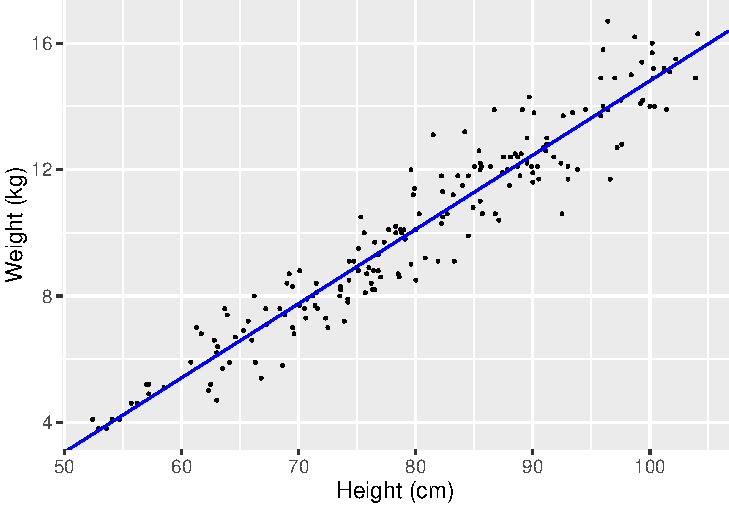
\includegraphics{RProgrammingForResearch_files/figure-latex/modelcoefplot-1} 

}

\caption{Example of using the output from a coefficients call to add a regression line to a scatterplot.}\label{fig:modelcoefplot}
\end{figure}

\begin{rmdnote}
You can also add a linear regression line to a scatterplot by adding the
geom \texttt{geom\_smooth} using the argument \texttt{method\ =\ "lm"}.
\end{rmdnote}

You can use the function \texttt{residuals} on an \texttt{lm} object to
pull out the residuals from the model fit:

\begin{Shaded}
\begin{Highlighting}[]
\KeywordTok{head}\NormalTok{(}\KeywordTok{residuals}\NormalTok{(mod_a))}
\end{Highlighting}
\end{Shaded}

\begin{verbatim}
##           1           2           3           4           5           6 
##  0.05820415 -0.82693141 -0.08223993  0.48644436 -0.46920621 -0.06405608
\end{verbatim}

The result of a \texttt{residuals} call is a vector with one element for
each of the non-missing observations (rows) in the dataframe you used to
fit the model. Each value gives the different between the model fitted
value and the observed value for each of these observations, in the same
order the observations show up in the dataframe. The residuals are in
the same order as the observations in the original dataframe.

\begin{rmdtip}
You can also use the shorter function \texttt{coef} as an alternative to
\texttt{coefficients} and the shorter function \texttt{resid} as an
alternative to \texttt{residuals}.
\end{rmdtip}

As noted in the subsection on simple statistics functions, the
\texttt{summary} function returns different output depending on the type
of object that is input to the function. If you input a regression model
object to \texttt{summary}, the function gives you a lot of information
about the model. For example, here is the output returned by running
\texttt{summary} for the linear regression model object we just created:

\begin{Shaded}
\begin{Highlighting}[]
\KeywordTok{summary}\NormalTok{(mod_a)}
\end{Highlighting}
\end{Shaded}

\begin{verbatim}
## 
## Call:
## lm(formula = wt ~ ht, data = nepali)
## 
## Residuals:
##      Min       1Q   Median       3Q      Max 
## -2.44736 -0.55708  0.01925  0.49941  2.73594 
## 
## Coefficients:
##              Estimate Std. Error t value Pr(>|t|)    
## (Intercept) -8.694768   0.427398  -20.34   <2e-16 ***
## ht           0.235050   0.005257   44.71   <2e-16 ***
## ---
## Signif. codes:  0 '***' 0.001 '**' 0.01 '*' 0.05 '.' 0.1 ' ' 1
## 
## Residual standard error: 0.9017 on 183 degrees of freedom
##   (15 observations deleted due to missingness)
## Multiple R-squared:  0.9161, Adjusted R-squared:  0.9157 
## F-statistic:  1999 on 1 and 183 DF,  p-value: < 2.2e-16
\end{verbatim}

This output includes a lot of useful elements, including (1) basic
summary statistics for the residuals (to meet model assumptions, the
median should be around zero and the absolute values fairly similar for
the first and third quantiles), (2) coefficient estimates, standard
errors, and p-values, and (3) some model summary statistics, including
residual standard error, degrees of freedom, number of missing
observations, and F-statistic.

The object returned by the \texttt{summary()} function when it is
applied to an \texttt{lm} object is a list, which you can confirm using
the \texttt{is.list} function:

\begin{Shaded}
\begin{Highlighting}[]
\KeywordTok{is.list}\NormalTok{(}\KeywordTok{summary}\NormalTok{(mod_a))}
\end{Highlighting}
\end{Shaded}

\begin{verbatim}
## [1] TRUE
\end{verbatim}

With any list, you can use the \texttt{names} function to get the names
of all of the different elements of the object:

\begin{Shaded}
\begin{Highlighting}[]
\KeywordTok{names}\NormalTok{(}\KeywordTok{summary}\NormalTok{(mod_a))}
\end{Highlighting}
\end{Shaded}

\begin{verbatim}
##  [1] "call"          "terms"         "residuals"     "coefficients" 
##  [5] "aliased"       "sigma"         "df"            "r.squared"    
##  [9] "adj.r.squared" "fstatistic"    "cov.unscaled"  "na.action"
\end{verbatim}

You can use the \texttt{\$} operator to pull out any element of the
list. For example, to pull out the table with information on the
estimated model coefficients, you can run:

\begin{Shaded}
\begin{Highlighting}[]
\KeywordTok{summary}\NormalTok{(mod_a)$coefficients}
\end{Highlighting}
\end{Shaded}

\begin{verbatim}
##              Estimate  Std. Error   t value      Pr(>|t|)
## (Intercept) -8.694768 0.427397843 -20.34350  7.424640e-49
## ht           0.235050 0.005256822  44.71334 1.962647e-100
\end{verbatim}

The \texttt{plot} function, like the \texttt{summary} function, will
give different output depending on the class of the object that you
input. For an \texttt{lm} object, you can use the \texttt{plot} function
to get a number of useful diagnostic plots that will help you check
regression assumptions (Figure \ref{fig:plotlmexample}):

\begin{Shaded}
\begin{Highlighting}[]
\KeywordTok{plot}\NormalTok{(mod_a)}
\end{Highlighting}
\end{Shaded}

\begin{figure}

{\centering 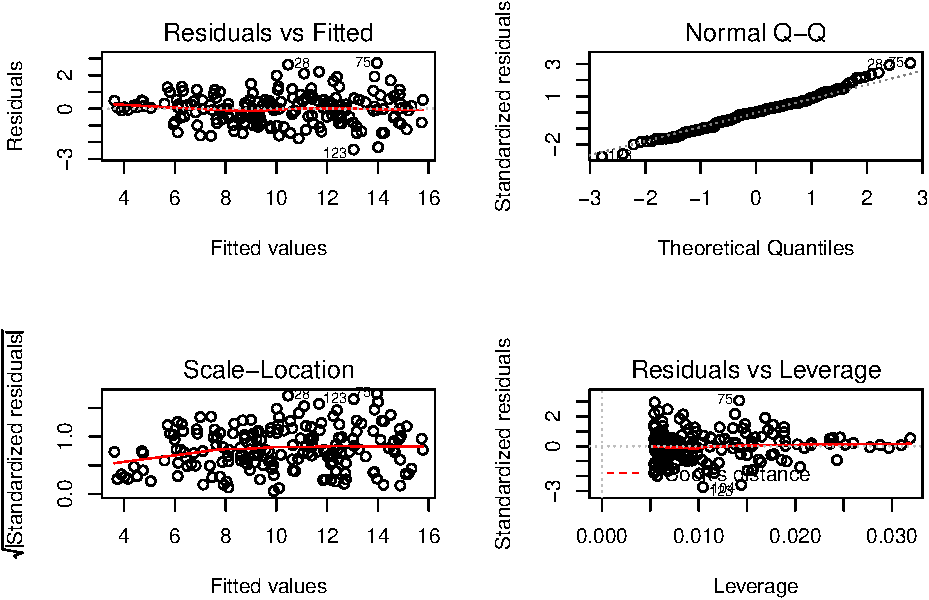
\includegraphics[width=\textwidth]{RProgrammingForResearch_files/figure-latex/plotlmexample-1} 

}

\caption{Example output from running the plot function with an lm object as the input.}\label{fig:plotlmexample}
\end{figure}

You can also use binary variables or factors as independent variables in
regression models. For example, in the \texttt{nepali} dataset,
\texttt{sex} is a factor variable with the levels ``Male'' and
``Female''. You can fit a linear model of weight regressed on sex for
this data with the call:

\begin{Shaded}
\begin{Highlighting}[]
\NormalTok{mod_b <-}\StringTok{ }\KeywordTok{lm}\NormalTok{(wt ~}\StringTok{ }\NormalTok{sex, }\DataTypeTok{data =} \NormalTok{nepali)}
\end{Highlighting}
\end{Shaded}

This call fits the model:

\[ Y_{i} = \beta_{0} + \beta_{1}X_{1,i} + \epsilon_{i} \]

where \(X_{1,i}\) : sex of child \(i\), where 0 = male and 1 = female.

Here are the estimated coefficients from fitting this model:

\begin{Shaded}
\begin{Highlighting}[]
\KeywordTok{summary}\NormalTok{(mod_b)$coefficients}
\end{Highlighting}
\end{Shaded}

\begin{verbatim}
##              Estimate Std. Error   t value     Pr(>|t|)
## (Intercept) 10.497980  0.3110957 33.745177 1.704550e-80
## sexFemale   -0.674724  0.4562792 -1.478752 1.409257e-01
\end{verbatim}

You'll notice that, in addition to an estimated intercept
(\texttt{(Intercept)}), the other estimated coefficient is
\texttt{sexFemale} rather than just \texttt{sex}, although the column
name in the dataframe input to \texttt{lm} for this variable is
\texttt{sex}.

This is because, when a factor or binary variable is input as an
independent variable in a linear regression model, R will fit an
estimated coefficient for all levels of factors \emph{except} the first
factor level. By default, this first factor level is used as the
baseline level, and so its estimated mean is given by the estimated
intercept, while the other model coefficients give the estimated
\emph{difference} from this baseline.

For example, the model fit above tells us that the estimated mean weight
of males is 10.5, while the estimated mean weight of females is 10.5 +
-0.7 = 9.8.

If you would prefer that a different level of the factor be the baseline
(for example, ``Female'' rather than ``Male'' for the previous
regression), you can do that by using the \texttt{levels} argument in
the \texttt{factor} function to reset factor levels. For example:

\begin{Shaded}
\begin{Highlighting}[]
\NormalTok{nepali_reset <-}\StringTok{ }\NormalTok{nepali %>%}
\StringTok{  }\KeywordTok{mutate}\NormalTok{(}\DataTypeTok{sex =} \KeywordTok{factor}\NormalTok{(sex, }\DataTypeTok{levels =} \KeywordTok{c}\NormalTok{(}\StringTok{"Female"}\NormalTok{, }\StringTok{"Male"}\NormalTok{)))}
\NormalTok{mod_b_reset <-}\StringTok{ }\KeywordTok{lm}\NormalTok{(wt ~}\StringTok{ }\NormalTok{sex, }\DataTypeTok{data =} \NormalTok{nepali_reset)}
\KeywordTok{summary}\NormalTok{(mod_b_reset)$coef}
\end{Highlighting}
\end{Shaded}

\begin{verbatim}
##             Estimate Std. Error   t value     Pr(>|t|)
## (Intercept) 9.823256  0.3337816 29.430189 2.626719e-71
## sexMale     0.674724  0.4562792  1.478752 1.409257e-01
\end{verbatim}

Now, \texttt{(Intercept)} gives the estimated mean weight for females,
while the second estimated coefficient gives the estimated mean
difference for males compared to the expected value for females.

\subsection{Generalized linear models
(GLMs)}\label{generalized-linear-models-glms}

You can fit a variety of models, including linear models, logistic
models, and Poisson models, using generalized linear models (GLMs).
\medskip

For linear models, the only difference between \texttt{lm} and
\texttt{glm} are the mechanics of how they estimate the model
coefficients (\texttt{lm} uses least squares while \texttt{glm} uses
maximum likelihood). You will (almost always) get exactly the same
estimated coefficients regardless of whether you use \texttt{glm} or
\texttt{lm} to fit a linear regression.

For example, here is the code to fit a linear regression model for
weight regressed on height from the \texttt{nepali} dataset:

\begin{Shaded}
\begin{Highlighting}[]
\NormalTok{mod_c <-}\StringTok{ }\KeywordTok{glm}\NormalTok{(wt ~}\StringTok{ }\NormalTok{ht, }\DataTypeTok{data =} \NormalTok{nepali)}
\end{Highlighting}
\end{Shaded}

This call fits the same regression model I fit earlier with the
\texttt{lm} function and saved as \texttt{mod\_a}. You can see that the
two methods give exactly the same coefficient estimates:

\begin{Shaded}
\begin{Highlighting}[]
\KeywordTok{coef}\NormalTok{(mod_c)}
\end{Highlighting}
\end{Shaded}

\begin{verbatim}
## (Intercept)          ht 
##   -8.694768    0.235050
\end{verbatim}

\begin{Shaded}
\begin{Highlighting}[]
\KeywordTok{coef}\NormalTok{(mod_a)}
\end{Highlighting}
\end{Shaded}

\begin{verbatim}
## (Intercept)          ht 
##   -8.694768    0.235050
\end{verbatim}

Unlike the \texttt{lm} function, however, the \texttt{glm} function also
allows you to fit other model types, including logistic and Poisson
models. You can specify the model type using the \texttt{family}
argument to the \texttt{glm} call:

\begin{tabular}{l|l}
\hline
Model type & `family` argument\\
\hline
Linear & `family = gaussian(link = 'identity')`\\
\hline
Logistic & `family = binomial(link = 'logit')`\\
\hline
Poisson & `family = poisson(link = 'log')`\\
\hline
\end{tabular}

For example, say we wanted to fit a logistic regression for the
\texttt{nepali} data of whether the probability of a child weighing more
than 13 kg is associated with the child's sex.

First, create a binary variable in the \texttt{nepali} dataset,
\texttt{wt\_over\_13}, that is \texttt{TRUE} if a child weighed more
than 13 kilograms and FALSE otherwise. You can use the \texttt{mutate}
function from \texttt{dplyr} to add this new column (which, as a note,
is a logical vector):

\begin{Shaded}
\begin{Highlighting}[]
\NormalTok{nepali <-}\StringTok{ }\NormalTok{nepali %>%}\StringTok{ }
\StringTok{  }\KeywordTok{mutate}\NormalTok{(}\DataTypeTok{wt_over_13 =} \NormalTok{wt >}\StringTok{ }\DecValTok{13}\NormalTok{)}
\KeywordTok{head}\NormalTok{(nepali)}
\end{Highlighting}
\end{Shaded}

\begin{verbatim}
##       id    sex   wt    ht age wt_over_13
## 1 120011   Male 12.8  91.2  41      FALSE
## 2 120012 Female 14.9 103.9  57       TRUE
## 3 120021 Female  7.7  70.1   8      FALSE
## 4 120022 Female 12.1  86.4  35      FALSE
## 5 120023   Male 14.2  99.4  49       TRUE
## 6 120031   Male 13.9  96.4  46       TRUE
\end{verbatim}

Now you can fit a logistic regression of \texttt{wt\_over\_13} regressed
on sex, using a logistic model:

\begin{Shaded}
\begin{Highlighting}[]
\NormalTok{mod_d <-}\StringTok{ }\KeywordTok{glm}\NormalTok{(wt_over_13 ~}\StringTok{ }\NormalTok{sex, }\DataTypeTok{data =} \NormalTok{nepali,}
             \DataTypeTok{family =} \KeywordTok{binomial}\NormalTok{(}\DataTypeTok{link =} \StringTok{"logit"}\NormalTok{))}
\end{Highlighting}
\end{Shaded}

Elements of a GLM can be pulled out in the same way that we looked at
elements from the linear model fit with \texttt{lm}. For example, to see
a table of estimated model coefficients, you can run:

\begin{Shaded}
\begin{Highlighting}[]
\KeywordTok{summary}\NormalTok{(mod_d)$coef}
\end{Highlighting}
\end{Shaded}

\begin{verbatim}
##               Estimate Std. Error   z value     Pr(>|z|)
## (Intercept) -1.3121864  0.2458445 -5.337465 9.425485e-08
## sexFemale   -0.4133237  0.3886659 -1.063442 2.875815e-01
\end{verbatim}

Because this model was a logistic model, fit with a log link, here the
model coefficient estimate for \texttt{sexFemale} gives an estimate of
the \textbf{log odds} of weight higher than 13 kg associated with
females versus males. The p-value for this estimate
(\texttt{Pr(\textgreater{}\textbar{}z\textbar{})} = 0.29) isn't very
small, suggesting that the difference between male and female children
in the odds of weighing more than 13 kg is not statistically
significant.

\subsection{References-- statistics in
R}\label{references-statistics-in-r}

One great (and free online for CSU students through our library) book to
find out more about using R for basic statistics is:

\begin{itemize}
\tightlist
\item
  \href{http://discovery.library.colostate.edu/Record/.b44705323}{Introductory
  Statistics with R}
\end{itemize}

If you want all the details about fitting linear models and GLMs in R,
Julian Faraway's books are fantastic. He has one on linear models and
one on extensions including logistic and Poisson models:

\begin{itemize}
\tightlist
\item
  \href{http://discovery.library.colostate.edu/Record/.b41119691}{Linear
  Models with R} (also free online through the CSU library)
\item
  \href{http://www.amazon.com/Extending-Linear-Model-Generalized-Nonparametric/dp/158488424X/ref=sr_1_1?ie=UTF8\&qid=1442252668\&sr=8-1\&keywords=extending+linear+model+r}{Extending
  the Linear Model with R}
\end{itemize}

\section{In-course exercise}\label{in-course-exercise-2}

\subsection{Loading data from an R
package}\label{loading-data-from-an-r-package}

The data we'll be using today is from a dataset called \texttt{worldcup}
in the package \texttt{faraway}. Load that data so you can use it on
your computer (note: you will need to load and install the
\texttt{faraway} package to do this). Use the help file for the data to
find out more about the dataset. Use some basic functions, like
\texttt{head}, \texttt{tail}, \texttt{colnames}, \texttt{str}, and
\texttt{summary} to check out the data a bit. See if you can figure out:

\begin{itemize}
\tightlist
\item
  What variables are included in this dataset? (Check the column names.)
\item
  What class is each column currently? In particular, which are numbers
  and which are factors?
\end{itemize}

\subsubsection{Example R code:}\label{example-r-code}

Load the \texttt{faraway} package using \texttt{load()} and then load
the data using \texttt{data()}:

\begin{Shaded}
\begin{Highlighting}[]
\NormalTok{## Uncomment the next line if you need to install the package}
\CommentTok{# install.packages("faraway")}
\KeywordTok{library}\NormalTok{(faraway)}
\KeywordTok{data}\NormalTok{(}\StringTok{"worldcup"}\NormalTok{)}
\end{Highlighting}
\end{Shaded}

Check out the help file for the \texttt{worldcup} dataset to find out
more about the data. (Note: Only datasets that are parts of packages
will have help files.)

\begin{Shaded}
\begin{Highlighting}[]
\NormalTok{?worldcup}
\end{Highlighting}
\end{Shaded}

Check out the data a bit:

\begin{Shaded}
\begin{Highlighting}[]
\KeywordTok{str}\NormalTok{(worldcup)}
\end{Highlighting}
\end{Shaded}

\begin{verbatim}
## 'data.frame':    595 obs. of  7 variables:
##  $ Team    : Factor w/ 32 levels "Algeria","Argentina",..: 1 16 9 9 5 32 11 11 18 20 ...
##  $ Position: Factor w/ 4 levels "Defender","Forward",..: 4 4 1 4 2 2 1 2 4 1 ...
##  $ Time    : int  16 351 180 270 46 72 138 33 21 103 ...
##  $ Shots   : int  0 0 0 1 2 0 0 0 5 0 ...
##  $ Passes  : int  6 101 91 111 16 15 51 9 22 38 ...
##  $ Tackles : int  0 14 6 5 0 0 2 0 0 1 ...
##  $ Saves   : int  0 0 0 0 0 0 0 0 0 0 ...
\end{verbatim}

\begin{Shaded}
\begin{Highlighting}[]
\KeywordTok{head}\NormalTok{(worldcup)}
\end{Highlighting}
\end{Shaded}

\begin{verbatim}
##                Team   Position Time Shots Passes Tackles Saves
## Abdoun      Algeria Midfielder   16     0      6       0     0
## Abe           Japan Midfielder  351     0    101      14     0
## Abidal       France   Defender  180     0     91       6     0
## Abou Diaby   France Midfielder  270     1    111       5     0
## Aboubakar  Cameroon    Forward   46     2     16       0     0
## Abreu       Uruguay    Forward   72     0     15       0     0
\end{verbatim}

\begin{Shaded}
\begin{Highlighting}[]
\KeywordTok{tail}\NormalTok{(worldcup)}
\end{Highlighting}
\end{Shaded}

\begin{verbatim}
##                        Team   Position Time Shots Passes Tackles Saves
## van Bommel      Netherlands Midfielder  540     2    307      31     0
## van Bronckhorst Netherlands   Defender  540     1    271      10     0
## van Persie      Netherlands    Forward  479    14    108       1     0
## von Bergen      Switzerland   Defender  234     0     79       3     0
## Alvaro Pereira      Uruguay Midfielder  409     6    140      17     0
## Ozil                Germany Midfielder  497     7    266       3     0
\end{verbatim}

\begin{Shaded}
\begin{Highlighting}[]
\KeywordTok{colnames}\NormalTok{(worldcup)}
\end{Highlighting}
\end{Shaded}

\begin{verbatim}
## [1] "Team"     "Position" "Time"     "Shots"    "Passes"   "Tackles" 
## [7] "Saves"
\end{verbatim}

\begin{Shaded}
\begin{Highlighting}[]
\KeywordTok{summary}\NormalTok{(worldcup)}
\end{Highlighting}
\end{Shaded}

\begin{verbatim}
##         Team           Position        Time           Shots       
##  Slovakia : 21   Defender  :188   Min.   :  1.0   Min.   : 0.000  
##  Uruguay  : 21   Forward   :143   1st Qu.: 88.0   1st Qu.: 0.000  
##  Argentina: 20   Goalkeeper: 36   Median :191.0   Median : 1.000  
##  Cameroon : 20   Midfielder:228   Mean   :208.9   Mean   : 2.304  
##  Chile    : 20                    3rd Qu.:270.0   3rd Qu.: 3.000  
##  Paraguay : 20                    Max.   :570.0   Max.   :27.000  
##  (Other)  :473                                                    
##      Passes          Tackles           Saves        
##  Min.   :  0.00   Min.   : 0.000   Min.   : 0.0000  
##  1st Qu.: 29.00   1st Qu.: 1.000   1st Qu.: 0.0000  
##  Median : 61.00   Median : 3.000   Median : 0.0000  
##  Mean   : 84.52   Mean   : 4.192   Mean   : 0.6672  
##  3rd Qu.:115.50   3rd Qu.: 6.000   3rd Qu.: 0.0000  
##  Max.   :563.00   Max.   :34.000   Max.   :20.0000  
## 
\end{verbatim}

\subsection{Basic plots of the data}\label{basic-plots-of-the-data}

Use some basic plots to check out this data. Try the following:

\begin{itemize}
\tightlist
\item
  Plot histograms of all the numeric variables (\texttt{Time},
  \texttt{Shot}, \texttt{Passes}, \texttt{Tackles}, \texttt{Saves})
\item
  Plot scatterplots of different combinations of numeric variables
  (e.g., \texttt{Time} vs. \texttt{Shots}). Try doing this using the
  \texttt{geom\_point()} geom from \texttt{ggplot2}. Also try doing it
  using the \texttt{ggpairs()} function from the \texttt{GGally}
  package, to plot several of these at the same time. Try using
  different constant or mapped values with the \texttt{color} aesthetic.
\item
  Create boxplots of \texttt{Time}, \texttt{Shots}, \texttt{Passes} and
  \texttt{Saves} by position.
\item
  Go online and find out which teams were the top four teams in this
  World Cup (i.e., first through fourth places). Create a
  \texttt{top\_teams} subset with just these teams. Plot boxplots of
  \texttt{Shots} and \texttt{Saves} by team for just these teams.
\item
  Did you notice any interesting features of the data when you did any
  of the graphs in this section?
\end{itemize}

\subsubsection{Example R code:}\label{example-r-code-1}

Use histograms to explore the distribution of different variables. If
you want to change the number of bins in the histogram, try playing
around with the \texttt{bins} and \texttt{binwidth} arguments. You can
use the \texttt{bins} argument to say how many bins you want (e.g.,
\texttt{bins\ =\ 50}). You can use the \texttt{binwidth} argument to say
how wide you want the bins to be (e.g., \texttt{binwidth\ =\ 10} if you
wanted bins to be 10 units wide, in the units of the variable mapped to
the \texttt{x} aesthetic. Try using \texttt{fill} and \texttt{color} to
change the appearance of the plot. Google ``R colors'' and search the
images to find links to listings of different R colors.

\begin{Shaded}
\begin{Highlighting}[]
\KeywordTok{library}\NormalTok{(ggplot2)}
\KeywordTok{ggplot}\NormalTok{(worldcup, }\KeywordTok{aes}\NormalTok{(}\DataTypeTok{x =} \NormalTok{Time)) +}\StringTok{ }
\StringTok{  }\KeywordTok{geom_histogram}\NormalTok{()}
\end{Highlighting}
\end{Shaded}

\begin{center}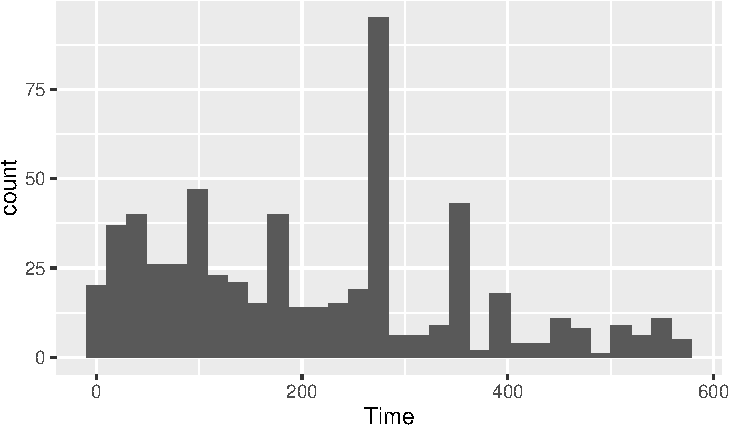
\includegraphics{RProgrammingForResearch_files/figure-latex/unnamed-chunk-191-1} \end{center}

\begin{Shaded}
\begin{Highlighting}[]
\KeywordTok{ggplot}\NormalTok{(worldcup, }\KeywordTok{aes}\NormalTok{(}\DataTypeTok{x =} \NormalTok{Time)) +}\StringTok{ }
\StringTok{  }\KeywordTok{geom_histogram}\NormalTok{(}\DataTypeTok{bins =} \DecValTok{50}\NormalTok{)}
\end{Highlighting}
\end{Shaded}

\begin{center}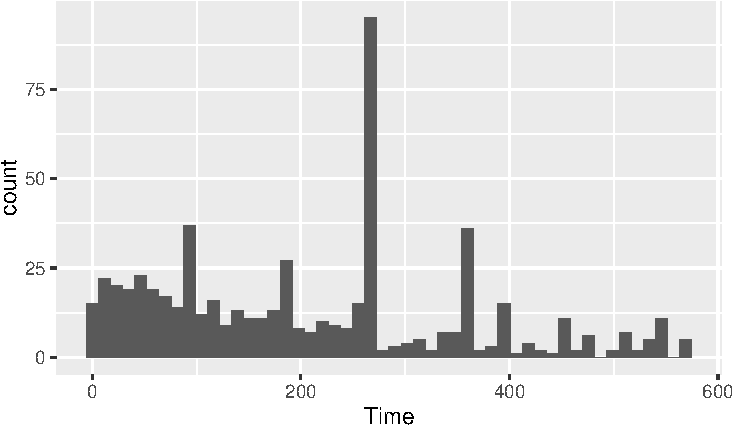
\includegraphics{RProgrammingForResearch_files/figure-latex/unnamed-chunk-191-2} \end{center}

\begin{Shaded}
\begin{Highlighting}[]
\KeywordTok{ggplot}\NormalTok{(worldcup, }\KeywordTok{aes}\NormalTok{(}\DataTypeTok{x =} \NormalTok{Time)) +}\StringTok{ }
\StringTok{  }\KeywordTok{geom_histogram}\NormalTok{(}\DataTypeTok{binwidth =} \DecValTok{100}\NormalTok{)}
\end{Highlighting}
\end{Shaded}

\begin{center}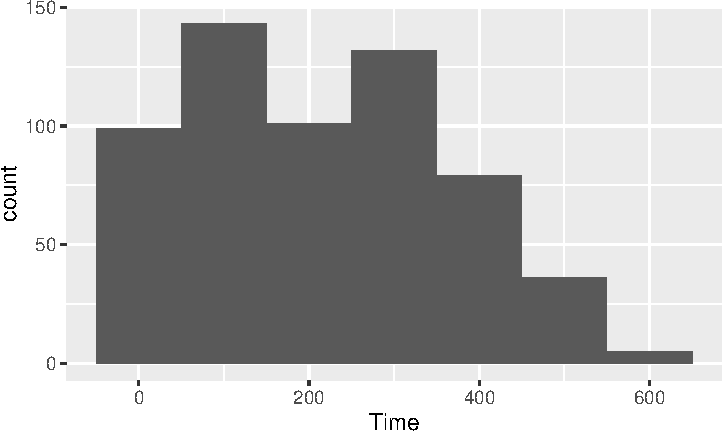
\includegraphics{RProgrammingForResearch_files/figure-latex/unnamed-chunk-191-3} \end{center}

\begin{Shaded}
\begin{Highlighting}[]
\KeywordTok{ggplot}\NormalTok{(worldcup, }\KeywordTok{aes}\NormalTok{(}\DataTypeTok{x =} \NormalTok{Time)) +}\StringTok{ }
\StringTok{  }\KeywordTok{geom_histogram}\NormalTok{(}\DataTypeTok{binwidth =} \DecValTok{50}\NormalTok{, }\DataTypeTok{color =} \StringTok{"white"}\NormalTok{, }\DataTypeTok{fill =} \StringTok{"cyan4"}\NormalTok{)}
\end{Highlighting}
\end{Shaded}

\begin{center}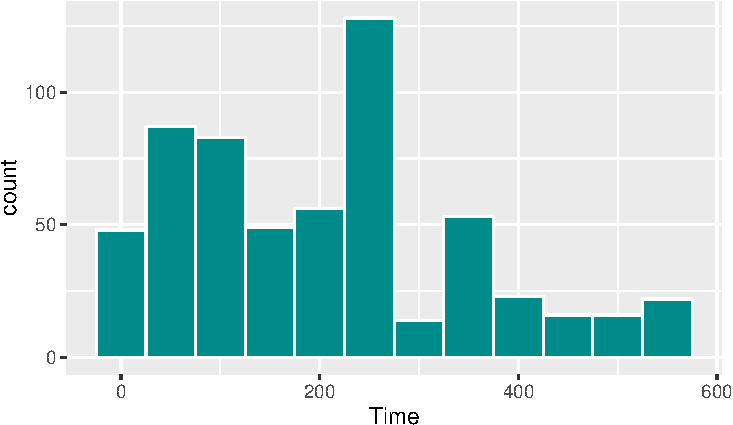
\includegraphics{RProgrammingForResearch_files/figure-latex/unnamed-chunk-191-4} \end{center}

Create a scatterplot of \texttt{Time} versus \texttt{Passes}. To change
the size of the points, use the \texttt{size} argument (use a number
lower than 1 for smaller points, higher than 1 for larger points). Try
changing the color and transparency of the points using the aesthetics
\texttt{color} and \texttt{alpha}. Try using color to show each player's
position by mapping \texttt{Position} to the \texttt{color} aesthetic.

\begin{Shaded}
\begin{Highlighting}[]
\KeywordTok{ggplot}\NormalTok{(worldcup, }\KeywordTok{aes}\NormalTok{(}\DataTypeTok{x =} \NormalTok{Time, }\DataTypeTok{y =} \NormalTok{Passes)) +}\StringTok{ }
\StringTok{  }\KeywordTok{geom_point}\NormalTok{()}
\end{Highlighting}
\end{Shaded}

\begin{center}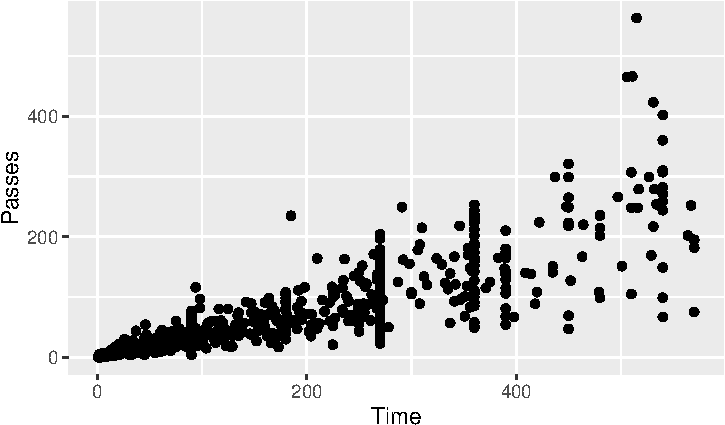
\includegraphics{RProgrammingForResearch_files/figure-latex/unnamed-chunk-192-1} \end{center}

\begin{Shaded}
\begin{Highlighting}[]
\KeywordTok{ggplot}\NormalTok{(worldcup, }\KeywordTok{aes}\NormalTok{(}\DataTypeTok{x =} \NormalTok{Time, }\DataTypeTok{y =} \NormalTok{Passes)) +}\StringTok{ }
\StringTok{  }\KeywordTok{geom_point}\NormalTok{(}\DataTypeTok{size =} \FloatTok{0.5}\NormalTok{)}
\end{Highlighting}
\end{Shaded}

\begin{center}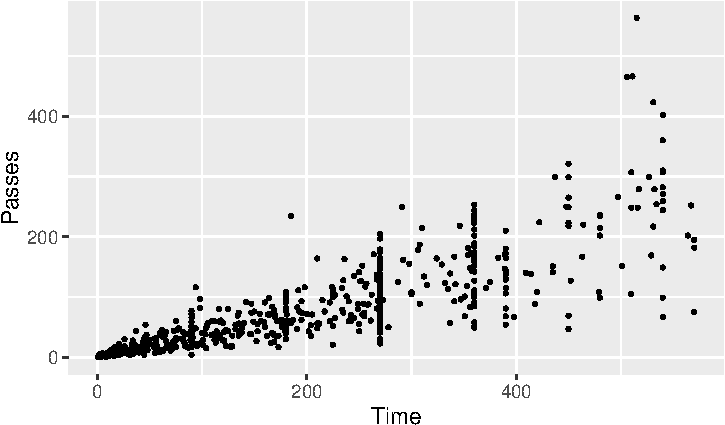
\includegraphics{RProgrammingForResearch_files/figure-latex/unnamed-chunk-192-2} \end{center}

\begin{Shaded}
\begin{Highlighting}[]
\KeywordTok{ggplot}\NormalTok{(worldcup, }\KeywordTok{aes}\NormalTok{(}\DataTypeTok{x =} \NormalTok{Time, }\DataTypeTok{y =} \NormalTok{Passes)) +}\StringTok{ }
\StringTok{  }\KeywordTok{geom_point}\NormalTok{(}\DataTypeTok{size =} \DecValTok{2}\NormalTok{, }\DataTypeTok{color =} \StringTok{"blue"}\NormalTok{, }\DataTypeTok{alpha =} \FloatTok{0.25}\NormalTok{)}
\end{Highlighting}
\end{Shaded}

\begin{center}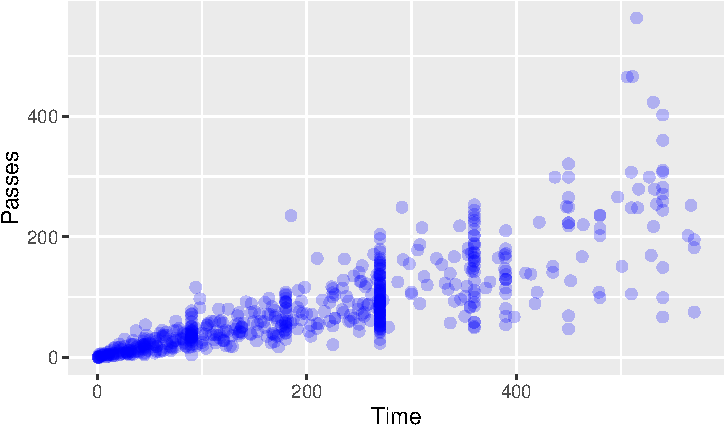
\includegraphics{RProgrammingForResearch_files/figure-latex/unnamed-chunk-192-3} \end{center}

\begin{Shaded}
\begin{Highlighting}[]
\KeywordTok{ggplot}\NormalTok{(worldcup, }\KeywordTok{aes}\NormalTok{(}\DataTypeTok{x =} \NormalTok{Time, }\DataTypeTok{y =} \NormalTok{Passes, }\DataTypeTok{color =} \NormalTok{Position)) +}\StringTok{ }
\StringTok{  }\KeywordTok{geom_point}\NormalTok{()}
\end{Highlighting}
\end{Shaded}

\begin{center}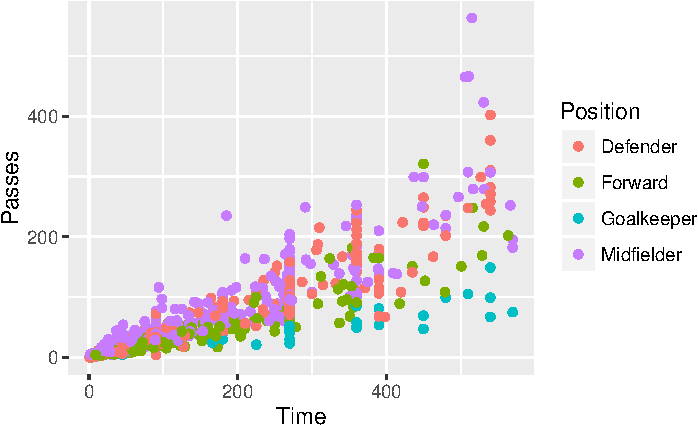
\includegraphics{RProgrammingForResearch_files/figure-latex/unnamed-chunk-192-4} \end{center}

Use the \texttt{ggpairs} function from the \texttt{GGally} package to
plot scatterplots of all combinations of several numeric variables.

\begin{Shaded}
\begin{Highlighting}[]
\KeywordTok{library}\NormalTok{(GGally)}
\KeywordTok{library}\NormalTok{(dplyr)}
\KeywordTok{ggpairs}\NormalTok{(}\KeywordTok{select}\NormalTok{(worldcup, Time, Shots, Passes, Tackles, Saves))}
\end{Highlighting}
\end{Shaded}

\begin{center}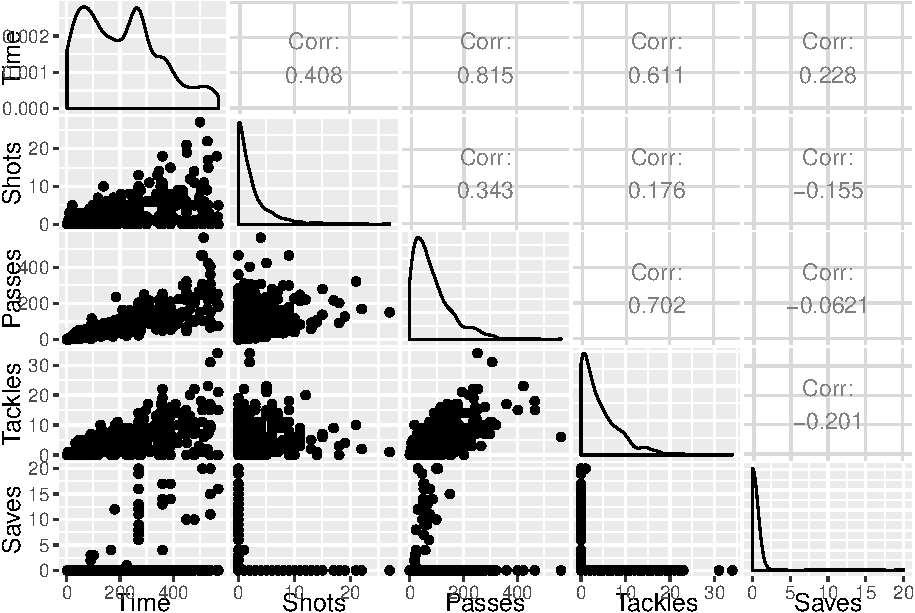
\includegraphics{RProgrammingForResearch_files/figure-latex/unnamed-chunk-193-1} \end{center}

To create a boxplot of \texttt{Shots} by \texttt{Position}, you can use
\texttt{geom\_boxplot}:

\begin{Shaded}
\begin{Highlighting}[]
\KeywordTok{ggplot}\NormalTok{(worldcup, }\KeywordTok{aes}\NormalTok{(}\DataTypeTok{x =} \NormalTok{Position, }\DataTypeTok{y =} \NormalTok{Shots)) +}\StringTok{ }
\StringTok{  }\KeywordTok{geom_boxplot}\NormalTok{()}
\end{Highlighting}
\end{Shaded}

\begin{center}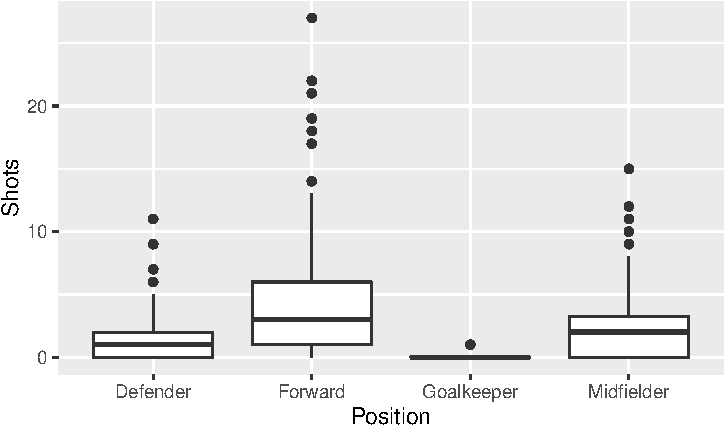
\includegraphics{RProgrammingForResearch_files/figure-latex/unnamed-chunk-194-1} \end{center}

The top four teams in this World Cup were Spain, the Netherlands,
Germany, and Uruguay. Create a subset with just the data for these four
teams:

\begin{Shaded}
\begin{Highlighting}[]
\NormalTok{top_teams <-}\StringTok{ }\NormalTok{worldcup %>%}
\StringTok{  }\KeywordTok{filter}\NormalTok{(Team %in%}\StringTok{ }\KeywordTok{c}\NormalTok{(}\StringTok{"Spain"}\NormalTok{, }\StringTok{"Netherlands"}\NormalTok{, }\StringTok{"Germany"}\NormalTok{, }\StringTok{"Uruguay"}\NormalTok{)) %>%}\StringTok{ }
\StringTok{  }\KeywordTok{mutate}\NormalTok{(}\DataTypeTok{Team =} \KeywordTok{factor}\NormalTok{(Team))}
\end{Highlighting}
\end{Shaded}

This dataset will still have all the levels saved for the \texttt{Team}
factor, even though it isn't using them all. You can re-set this by
resetting \texttt{Team} as a factor, which is what I've done with the
\texttt{mutate} line. When R creates a factor from a vector, its default
is to only use as levels the values that show up in the vector.

Now, you can plot the boxplots, mapping \texttt{Team} to the \texttt{x}
aesthetic and \texttt{Shots} or \texttt{Saves} to the \texttt{y}
aesthetic:

\begin{Shaded}
\begin{Highlighting}[]
\KeywordTok{ggplot}\NormalTok{(top_teams, }\KeywordTok{aes}\NormalTok{(}\DataTypeTok{x =} \NormalTok{Team, }\DataTypeTok{y =} \NormalTok{Shots)) +}\StringTok{ }
\StringTok{  }\KeywordTok{geom_boxplot}\NormalTok{() +}\StringTok{ }
\StringTok{  }\KeywordTok{ggtitle}\NormalTok{(}\StringTok{"Shots"}\NormalTok{)}
\end{Highlighting}
\end{Shaded}

\begin{center}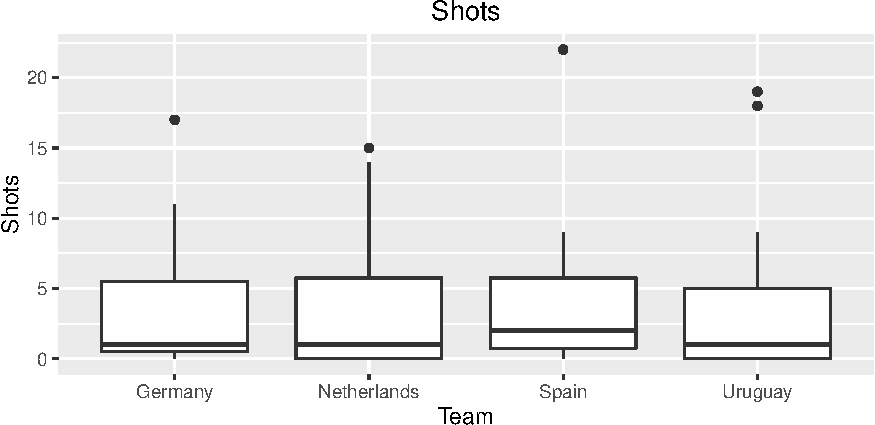
\includegraphics{RProgrammingForResearch_files/figure-latex/unnamed-chunk-196-1} \end{center}

\begin{Shaded}
\begin{Highlighting}[]
\KeywordTok{ggplot}\NormalTok{(top_teams, }\KeywordTok{aes}\NormalTok{(}\DataTypeTok{x =} \NormalTok{Team, }\DataTypeTok{y =} \NormalTok{Saves)) +}\StringTok{ }
\StringTok{  }\KeywordTok{geom_boxplot}\NormalTok{() +}\StringTok{ }
\StringTok{  }\KeywordTok{ggtitle}\NormalTok{(}\StringTok{"Saves"}\NormalTok{)}
\end{Highlighting}
\end{Shaded}

\begin{center}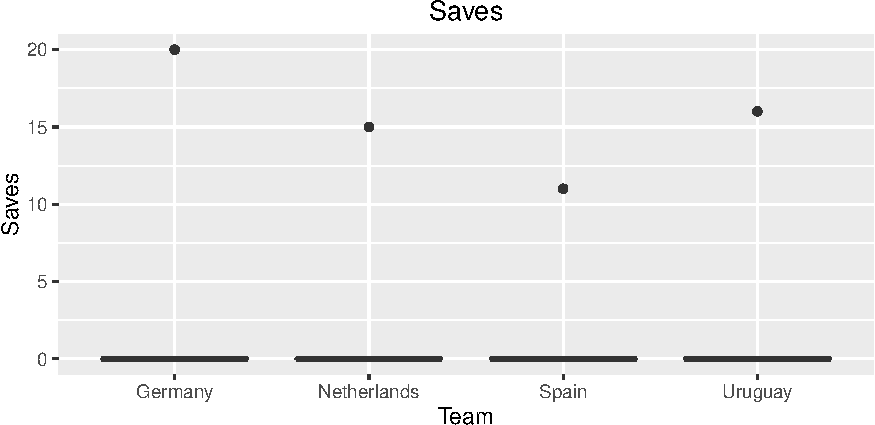
\includegraphics{RProgrammingForResearch_files/figure-latex/unnamed-chunk-196-2} \end{center}

\subsubsection{If you have extra time:}\label{if-you-have-extra-time}

If you wanted to do the same plot for several different variables, you
could loop through your code (we'll be covering more about loops in a
few weeks). For example, you could create histograms for all of the
numeric variables (if you do this in RStudio, you'll need to use the
arrows on the plot window to move through and see all the different
plots once you've created them):

\begin{Shaded}
\begin{Highlighting}[]
\NormalTok{## Create an object with the column names for all of the numeric variables}
\NormalTok{my_vars <-}\StringTok{ }\KeywordTok{colnames}\NormalTok{(worldcup)[}\DecValTok{3}\NormalTok{:}\DecValTok{7}\NormalTok{]}

\NormalTok{## Loop through all of those variables. Print out a histogram with the }
\NormalTok{## variable, and have it print on the plot, as the main title, the }
\NormalTok{## column name for that variable}
\NormalTok{for(var in my_vars)\{}
  \NormalTok{worldcup$to_plot <-}\StringTok{ }\NormalTok{worldcup[ , var]}
  \NormalTok{a <-}\StringTok{ }\KeywordTok{ggplot}\NormalTok{(worldcup, }\KeywordTok{aes}\NormalTok{(}\DataTypeTok{x =} \NormalTok{to_plot)) +}\StringTok{ }
\StringTok{    }\KeywordTok{geom_histogram}\NormalTok{(}\DataTypeTok{bins =} \DecValTok{20}\NormalTok{, }\DataTypeTok{color =} \StringTok{"white"}\NormalTok{, }\DataTypeTok{fill =} \StringTok{"navy"}\NormalTok{) +}\StringTok{ }
\StringTok{    }\KeywordTok{xlab}\NormalTok{(var) +}\StringTok{ }
\StringTok{    }\KeywordTok{ggtitle}\NormalTok{(}\KeywordTok{paste}\NormalTok{(}\StringTok{"Histogram of"}\NormalTok{, var))}
  \KeywordTok{plot}\NormalTok{(a)}
\NormalTok{\}}
\end{Highlighting}
\end{Shaded}

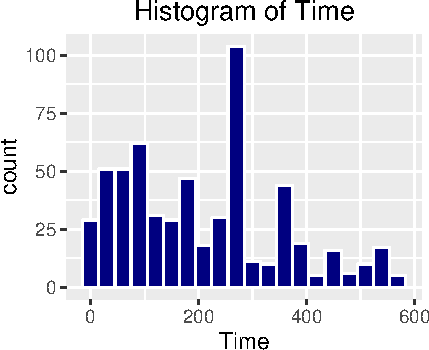
\includegraphics{RProgrammingForResearch_files/figure-latex/unnamed-chunk-197-1.pdf}
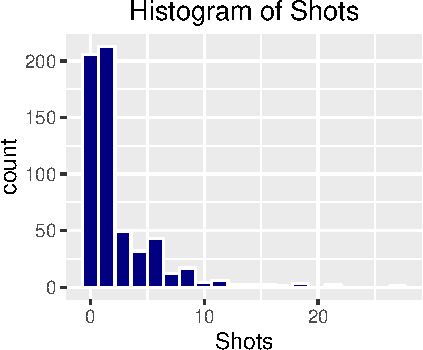
\includegraphics{RProgrammingForResearch_files/figure-latex/unnamed-chunk-197-2.pdf}
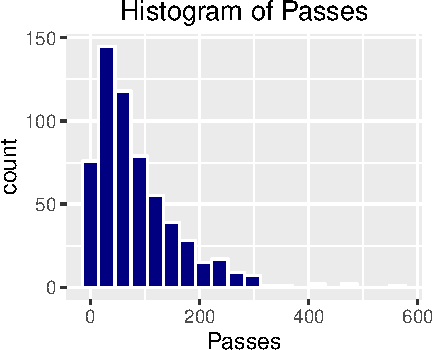
\includegraphics{RProgrammingForResearch_files/figure-latex/unnamed-chunk-197-3.pdf}
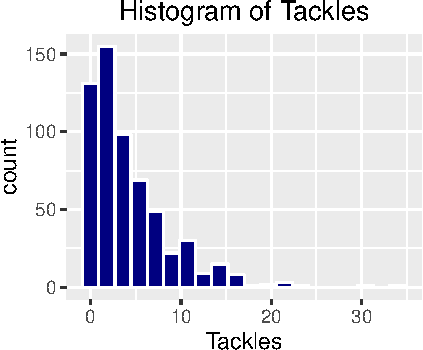
\includegraphics{RProgrammingForResearch_files/figure-latex/unnamed-chunk-197-4.pdf}
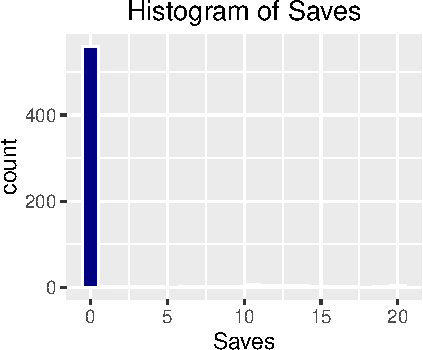
\includegraphics{RProgrammingForResearch_files/figure-latex/unnamed-chunk-197-5.pdf}

A few things to note in this example:

\begin{itemize}
\tightlist
\item
  To map an element of the data to an aesthetic, it's easiest if that
  element is saved in a column in the dataframe. Within this loop, I'm
  making an extra column called \texttt{to\_plot}, where I'm copying the
  column of the variable I want to plot each time the loop runs. That
  way, I can always use \texttt{x\ =\ to\_plot} in the aesthetic mapping
  for the ggplot object.
\item
  If you run code to create a ggplot object within a loop, it won't
  automatically print. Instead, you need to use \texttt{print} to get
  the object to print out. One way to do that is to save the final
  ggplot object as an R object (here I'm saving it to \texttt{a}) and
  then use the \texttt{print} function to print that object.
\item
  Next week, we'll talk some about faceting, which can create multiple
  plots by variable like this in a lot less code. However, it's useful
  at this point to start thinking about how to extend code to use in
  loops, to save yourself time when you need to repeat something similar
  many times.
\end{itemize}

\subsection{Exploring the data using simple statistics and logical
statements}\label{exploring-the-data-using-simple-statistics-and-logical-statements}

Next, try checking out the data using some basic commands for simple
statistics, like \texttt{mean()}, \texttt{range()}, \texttt{max()}, and
\texttt{min()}. Use these, along with some logical statements, to help
you answer the following questions:

\begin{itemize}
\tightlist
\item
  What is the range of time that players spent in the game? Who played
  the most World Cup time in this World Cup? For the minimum of the
  range of \texttt{Time}, how many players played this amount of time?
\item
  What is the mean number of saves that players made? What is the mean
  number of saves just among the goalkeepers? How many of the players
  are goalkeepers? Did any non-goalkeeper make a save?
\end{itemize}

\subsubsection{Example R code:}\label{example-r-code-2}

Use \texttt{range()} to find out the range of time these players played
in the World Cup.

\begin{Shaded}
\begin{Highlighting}[]
\KeywordTok{range}\NormalTok{(worldcup$Time)}
\end{Highlighting}
\end{Shaded}

\begin{verbatim}
## [1]   1 570
\end{verbatim}

To figure out who played the most time, you need to subset out the rows
of the dataset where the \texttt{Time} variable equals the maximum of
the \texttt{Time} variable for the whole dataset. There are a few ways
to do that. Here I'm showing two: (1) using logic within the
``square-bracket indexing'', to pull out just rows where it is TRUE that
the \texttt{Time} for that row equals \texttt{max(worldcup\$Time)} and
(2) using \texttt{filter} from the \texttt{dplyr} package to filter down
to rows where where it is TRUE that the \texttt{Time} for that row
equals \texttt{max(Time)} for the whole dataset.

\begin{Shaded}
\begin{Highlighting}[]
\KeywordTok{max}\NormalTok{(worldcup$Time)}
\end{Highlighting}
\end{Shaded}

\begin{verbatim}
## [1] 570
\end{verbatim}

\begin{Shaded}
\begin{Highlighting}[]
\KeywordTok{head}\NormalTok{(worldcup$Time ==}\StringTok{ }\KeywordTok{max}\NormalTok{(worldcup$Time))}
\end{Highlighting}
\end{Shaded}

\begin{verbatim}
## [1] FALSE FALSE FALSE FALSE FALSE FALSE
\end{verbatim}

\begin{Shaded}
\begin{Highlighting}[]
\NormalTok{worldcup[worldcup$Time ==}\StringTok{ }\KeywordTok{max}\NormalTok{(worldcup$Time), ]}
\end{Highlighting}
\end{Shaded}

\begin{verbatim}
##                 Team   Position Time Shots Passes Tackles Saves to_plot
## Arevalo Rios Uruguay Midfielder  570     5    195      21     0       0
## Maxi Pereira Uruguay Midfielder  570     5    182      15     0       0
## Muslera      Uruguay Goalkeeper  570     0     75       0    16      16
\end{verbatim}

\begin{Shaded}
\begin{Highlighting}[]
\NormalTok{worldcup %>%}
\StringTok{  }\KeywordTok{filter}\NormalTok{(Time ==}\StringTok{ }\KeywordTok{max}\NormalTok{(Time))}
\end{Highlighting}
\end{Shaded}

\begin{verbatim}
##      Team   Position Time Shots Passes Tackles Saves to_plot
## 1 Uruguay Midfielder  570     5    195      21     0       0
## 2 Uruguay Midfielder  570     5    182      15     0       0
## 3 Uruguay Goalkeeper  570     0     75       0    16      16
\end{verbatim}

\emph{Note}: You may have noticed that you lost the players names when
you did this using the \texttt{dplyr} pipechain. That's because
\texttt{dplyr} functions convert the data to a dataframe format that
does not include rownames. If you want to keep players' names, use
\texttt{mutate} to move those names from the rownames of the data into a
column in the dataframe:

\begin{Shaded}
\begin{Highlighting}[]
\NormalTok{worldcup %>%}
\StringTok{  }\KeywordTok{mutate}\NormalTok{(}\DataTypeTok{Name =} \KeywordTok{rownames}\NormalTok{(worldcup)) %>%}
\StringTok{  }\KeywordTok{filter}\NormalTok{(Time ==}\StringTok{ }\KeywordTok{max}\NormalTok{(Time))}
\end{Highlighting}
\end{Shaded}

\begin{verbatim}
##      Team   Position Time Shots Passes Tackles Saves to_plot         Name
## 1 Uruguay Midfielder  570     5    195      21     0       0 Arevalo Rios
## 2 Uruguay Midfielder  570     5    182      15     0       0 Maxi Pereira
## 3 Uruguay Goalkeeper  570     0     75       0    16      16      Muslera
\end{verbatim}

To calculate the mean number of saves among all the players, use the
\texttt{mean} function, either by itself or within a \texttt{summarize}
call:

\begin{Shaded}
\begin{Highlighting}[]
\KeywordTok{mean}\NormalTok{(worldcup$Saves)}
\end{Highlighting}
\end{Shaded}

\begin{verbatim}
## [1] 0.6672269
\end{verbatim}

\begin{Shaded}
\begin{Highlighting}[]
\NormalTok{worldcup %>%}
\StringTok{  }\KeywordTok{summarize}\NormalTok{(}\DataTypeTok{mean_saves =} \KeywordTok{mean}\NormalTok{(Saves))}
\end{Highlighting}
\end{Shaded}

\begin{verbatim}
##   mean_saves
## 1  0.6672269
\end{verbatim}

For the next parts of the question, it will be convenient to have a
logical vector for whether each player is a goalkeeper, so here's how
you would create that:

\begin{Shaded}
\begin{Highlighting}[]
\NormalTok{goalie <-}\StringTok{ }\NormalTok{worldcup$Position ==}\StringTok{ "Goalkeeper"}
\end{Highlighting}
\end{Shaded}

This new object, \texttt{goalie}, is a vector the same length as
\texttt{worldcup\$Position}. Each element of \texttt{goalie} says
whether it is TRUE or FALSE that \texttt{worldcup\$Position} is equal to
``Goalkeeper'' at that spot on the \texttt{worldcup\$Position} vector.

\begin{Shaded}
\begin{Highlighting}[]
\KeywordTok{head}\NormalTok{(goalie)}
\end{Highlighting}
\end{Shaded}

\begin{verbatim}
## [1] FALSE FALSE FALSE FALSE FALSE FALSE
\end{verbatim}

The \texttt{summary()} function will count up the total number of times
that \texttt{goalie} is TRUE and FALSE.

\begin{Shaded}
\begin{Highlighting}[]
\KeywordTok{summary}\NormalTok{(goalie)}
\end{Highlighting}
\end{Shaded}

\begin{verbatim}
##    Mode   FALSE    TRUE    NA's 
## logical     559      36       0
\end{verbatim}

There are a few ways to use this vector to figure out how many players
were goalkeepers. First, you could use \texttt{summary} (which I just
showed) or \texttt{table}, and just read how many times this vector has
the value \texttt{TRUE}. Second, since R saves logical vectors with
\texttt{TRUE} as 1 and \texttt{FALSE} as 0, you could just the
\texttt{sum} function to add up the vector to find out how often it's
\texttt{TRUE} (\texttt{sum} adds up every value in the vector).

\begin{Shaded}
\begin{Highlighting}[]
\KeywordTok{table}\NormalTok{(goalie)}
\end{Highlighting}
\end{Shaded}

\begin{verbatim}
## goalie
## FALSE  TRUE 
##   559    36
\end{verbatim}

\begin{Shaded}
\begin{Highlighting}[]
\KeywordTok{sum}\NormalTok{(goalie)}
\end{Highlighting}
\end{Shaded}

\begin{verbatim}
## [1] 36
\end{verbatim}

You could also answer this question by using \texttt{summarize} from
\texttt{dplyr}. You need to \texttt{group\_by} player position and then
you can use the \texttt{n} function in \texttt{summarize} to count up
the total number of observations in each group:

\begin{Shaded}
\begin{Highlighting}[]
\NormalTok{worldcup %>%}
\StringTok{  }\KeywordTok{group_by}\NormalTok{(Position) %>%}
\StringTok{  }\KeywordTok{summarize}\NormalTok{(}\DataTypeTok{n_players =} \KeywordTok{n}\NormalTok{())}
\end{Highlighting}
\end{Shaded}

\begin{verbatim}
## # A tibble: 4 × 2
##     Position n_players
##       <fctr>     <int>
## 1   Defender       188
## 2    Forward       143
## 3 Goalkeeper        36
## 4 Midfielder       228
\end{verbatim}

Now, you can answer the questions about mean saves for goalies and max
saves for non-goalies. First, try doing that using the \texttt{goalie}
logical vector you created. If you put \texttt{goalie} in the square
bracket indexing for the dataframe as the rows value (i.e., the index
before the comma), R will subset out just the rows where \texttt{goalie}
is equal to TRUE. If you put \texttt{!goalie} in the square bracket
indexing as the rows value, R will just subset out the rows where
\texttt{goalie} is equal to FALSE. You can use this index subsetting to
figure out the mean number of saves per goalie and also whether any
non-goalie made a save (by checking the maximum value or range of saves
for non-goalies).

\begin{Shaded}
\begin{Highlighting}[]
\KeywordTok{head}\NormalTok{(worldcup[goalie, ])}
\end{Highlighting}
\end{Shaded}

\begin{verbatim}
##                 Team   Position Time Shots Passes Tackles Saves to_plot
## Barry    Ivory Coast Goalkeeper  270     0     23       0     8       8
## Benaglio Switzerland Goalkeeper  270     0     75       0    11      11
## Bravo          Chile Goalkeeper  360     0     58       0     4       4
## Buffon         Italy Goalkeeper   45     0      4       0     0       0
## Casillas       Spain Goalkeeper  540     0     67       0    11      11
## Chaouchi     Algeria Goalkeeper   90     0     17       0     2       2
\end{verbatim}

\begin{Shaded}
\begin{Highlighting}[]
\KeywordTok{mean}\NormalTok{(worldcup[goalie, }\StringTok{"Saves"}\NormalTok{])}
\end{Highlighting}
\end{Shaded}

\begin{verbatim}
## [1] 11.02778
\end{verbatim}

\begin{Shaded}
\begin{Highlighting}[]
\KeywordTok{range}\NormalTok{(worldcup[!goalie, }\StringTok{"Saves"}\NormalTok{])}
\end{Highlighting}
\end{Shaded}

\begin{verbatim}
## [1] 0 0
\end{verbatim}

You could also answer this quesiton using a \texttt{dplyr} pipe chain to
summarize the data after grouping it by position:

\begin{Shaded}
\begin{Highlighting}[]
\NormalTok{worldcup %>%}
\StringTok{  }\KeywordTok{group_by}\NormalTok{(Position) %>%}
\StringTok{  }\KeywordTok{summarize}\NormalTok{(}\DataTypeTok{number_players =} \KeywordTok{n}\NormalTok{(), }
            \DataTypeTok{mean_saves =} \KeywordTok{mean}\NormalTok{(Saves),}
            \DataTypeTok{max_saves =} \KeywordTok{max}\NormalTok{(Saves))}
\end{Highlighting}
\end{Shaded}

\begin{verbatim}
## # A tibble: 4 × 4
##     Position number_players mean_saves max_saves
##       <fctr>          <int>      <dbl>     <int>
## 1   Defender            188    0.00000         0
## 2    Forward            143    0.00000         0
## 3 Goalkeeper             36   11.02778        20
## 4 Midfielder            228    0.00000         0
\end{verbatim}

\subsection{Using regression models to explore
data}\label{using-regression-models-to-explore-data}

For this part of the exercise, you'll use a dataset on weather, air
pollution, and mortality counts in Chicago, IL. This dataset is called
\texttt{chicagoNMMAPS} and is part of the \texttt{dlnm} package. Change
the name of the dataframe to something shorter, like \texttt{chic}.
Check out the data a bit to see what variables you have, and then
perform the following tasks:

\begin{itemize}
\tightlist
\item
  Write out (on paper, not in R) the regression equation for regressing
  dewpoint temperature on temperature.
\item
  Try fitting a linear regression of dew point temperature
  (\texttt{dptp}) on temperature (\texttt{temp}). (Bonus points: Notice
  anything that seems unusual about these two variables in this dataset?
  You can find out with \texttt{summary}, but it helps if you know a bit
  about what dewpoint temperature measures.) Save this model as the
  object \texttt{mod\_1}.
\item
  Based on this regression, does there seem to be a relationship between
  temperature and dewpoint temperature in Chicago? (Hint: Try using
  \texttt{summary()} on the model object to get more information about
  the model you fit.) What is the p-value for the coefficient for
  temperature?
\item
  Plot temperature (x-axis) versus dewpoint temperature (y-axis) for
  Chicago. Add in the regression line from the model you fit.
\item
  Use \texttt{plot()} on the model object to check if some of the
  assumptions for the regression model seem appropriate.
\item
  Try fitting the regression as a GLM, using \texttt{glm()}. Are your
  coefficients different?
\item
  Does \(PM_{10}\) vary by day of the week? (Hint: The \texttt{dow}
  variable is a factor that gives day of the week. You can do an ANOVA
  analysis by fitting a linear model using this variable as the
  independent variable, and then run \texttt{anova()} on that model, and
  R will compare it to an intercept-only model.) What day of the week is
  PM10 generally highest? (Check the model coefficients to figure this
  out.) Try to write out (on paper) the regression equation for the
  model you're fitting.
\item
  Try using \texttt{glm()} to run a Poisson regression of respiratory
  deaths (\texttt{resp}) on temperature during summer days. Start by
  creating a subset with just summer days called \texttt{summer}. (Hint:
  Use the \texttt{month} variable to do this-- just pull out the subset
  where the month is 6, 7, or 8, for June, July, and August.) Try to
  write out the regression equation for the model you're fitting.
\item
  The coefficient for the temperature variable in this model is our best
  estimate (based on this model) of the \textbf{log relative risk} for a
  one degree Celcius increase in temperature. What is the
  \textbf{relative risk} associated with a one degree Celsius increase?
\end{itemize}

\subsubsection{Example R code:}\label{example-r-code-3}

Install and load the \texttt{dlnm} package and then load the
\texttt{chicagoNMMAPS} data. Change the name of the dataframe to
\texttt{chic}, so it will be shorter to call for the rest of your work.

\begin{Shaded}
\begin{Highlighting}[]
\CommentTok{# install.packages("dlnm")}
\KeywordTok{library}\NormalTok{(dlnm)}
\KeywordTok{data}\NormalTok{(}\StringTok{"chicagoNMMAPS"}\NormalTok{)}
\NormalTok{chic <-}\StringTok{ }\NormalTok{chicagoNMMAPS}
\end{Highlighting}
\end{Shaded}

Fit a linear regression of \texttt{dptp} on \texttt{temp} and save as
the object \texttt{mod\_1}:

\begin{Shaded}
\begin{Highlighting}[]
\NormalTok{mod_1 <-}\StringTok{ }\KeywordTok{lm}\NormalTok{(dptp ~}\StringTok{ }\NormalTok{temp, }\DataTypeTok{data =} \NormalTok{chic)}
\NormalTok{mod_1}
\end{Highlighting}
\end{Shaded}

\begin{verbatim}
## 
## Call:
## lm(formula = dptp ~ temp, data = chic)
## 
## Coefficients:
## (Intercept)         temp  
##      24.025        1.621
\end{verbatim}

Use \texttt{summary()} to check out a bit more about the model you fit.

\begin{Shaded}
\begin{Highlighting}[]
\KeywordTok{summary}\NormalTok{(mod_1)}
\end{Highlighting}
\end{Shaded}

\begin{verbatim}
## 
## Call:
## lm(formula = dptp ~ temp, data = chic)
## 
## Residuals:
##      Min       1Q   Median       3Q      Max 
## -24.3093  -3.7470   0.4687   4.0738  18.6518 
## 
## Coefficients:
##              Estimate Std. Error t value Pr(>|t|)    
## (Intercept) 24.024869   0.112933   212.7   <2e-16 ***
## temp         1.620650   0.007631   212.4   <2e-16 ***
## ---
## Signif. codes:  0 '***' 0.001 '**' 0.01 '*' 0.05 '.' 0.1 ' ' 1
## 
## Residual standard error: 5.899 on 5112 degrees of freedom
## Multiple R-squared:  0.8982, Adjusted R-squared:  0.8982 
## F-statistic: 4.511e+04 on 1 and 5112 DF,  p-value: < 2.2e-16
\end{verbatim}

There does seem to be an association between temperature and dewpoint
temperature: a unit increase in temperature is associated with a 1.6
unit increase in dewpoint temperature. The p-value for the temperature
coefficient is \textless{}2e-16. This is far below 0.05, which suggests
we would be very unlikely to see such a strong association by chance if
the null hypothesis, that the two variables are not associated, were
true.

Plot these two variables and add in the regression line from the model
(note: I've used the \texttt{color} option to make the color of the
points gray). Use the values from \texttt{coef} with a
\texttt{geom\_abline} to add the regression line for the model you fit.

\begin{Shaded}
\begin{Highlighting}[]
\NormalTok{mod_coefs <-}\StringTok{ }\KeywordTok{coef}\NormalTok{(mod_1)}
\KeywordTok{ggplot}\NormalTok{(chic, }\KeywordTok{aes}\NormalTok{(}\DataTypeTok{x =} \NormalTok{temp, }\DataTypeTok{y =} \NormalTok{dptp)) +}\StringTok{ }
\StringTok{  }\KeywordTok{geom_point}\NormalTok{(}\DataTypeTok{size =} \FloatTok{0.5}\NormalTok{, }\DataTypeTok{col =} \StringTok{"gray"}\NormalTok{) +}\StringTok{ }
\StringTok{  }\KeywordTok{geom_abline}\NormalTok{(}\KeywordTok{aes}\NormalTok{(}\DataTypeTok{intercept =} \NormalTok{mod_coefs[}\DecValTok{1}\NormalTok{], }\DataTypeTok{slope =} \NormalTok{mod_coefs[}\DecValTok{2}\NormalTok{]))}
\end{Highlighting}
\end{Shaded}

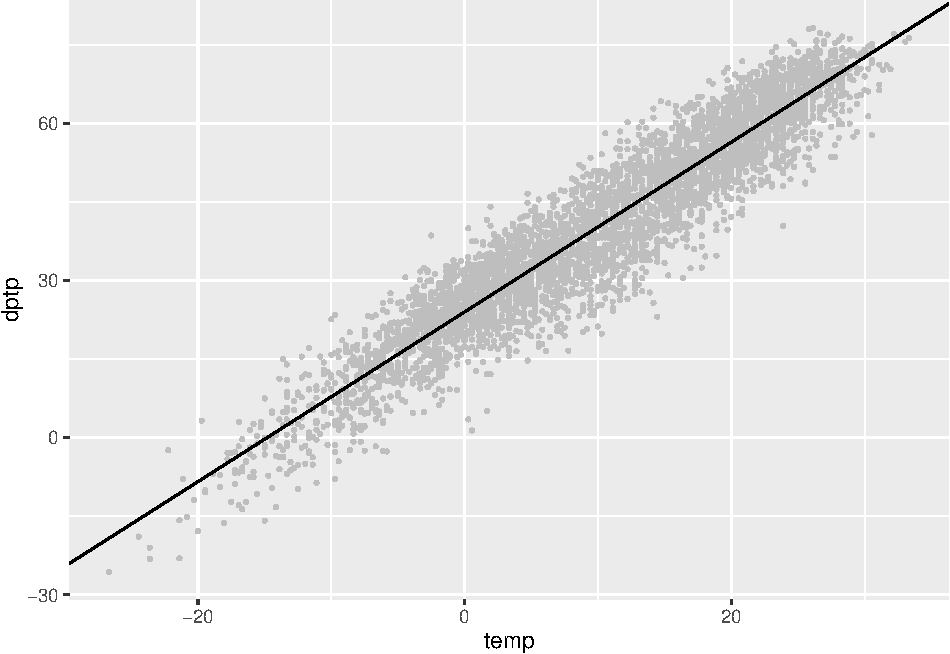
\includegraphics{RProgrammingForResearch_files/figure-latex/unnamed-chunk-212-1.pdf}

Plot some plots to check model assumptions for the model you fit using
the \texttt{plot()} function on your model object:

\begin{Shaded}
\begin{Highlighting}[]
\KeywordTok{par}\NormalTok{(}\DataTypeTok{mfrow =} \KeywordTok{c}\NormalTok{(}\DecValTok{2}\NormalTok{, }\DecValTok{2}\NormalTok{)) }\CommentTok{# Set to four plots per panel -- 2 rows, 2 columns}
\KeywordTok{plot}\NormalTok{(mod_1)}
\end{Highlighting}
\end{Shaded}

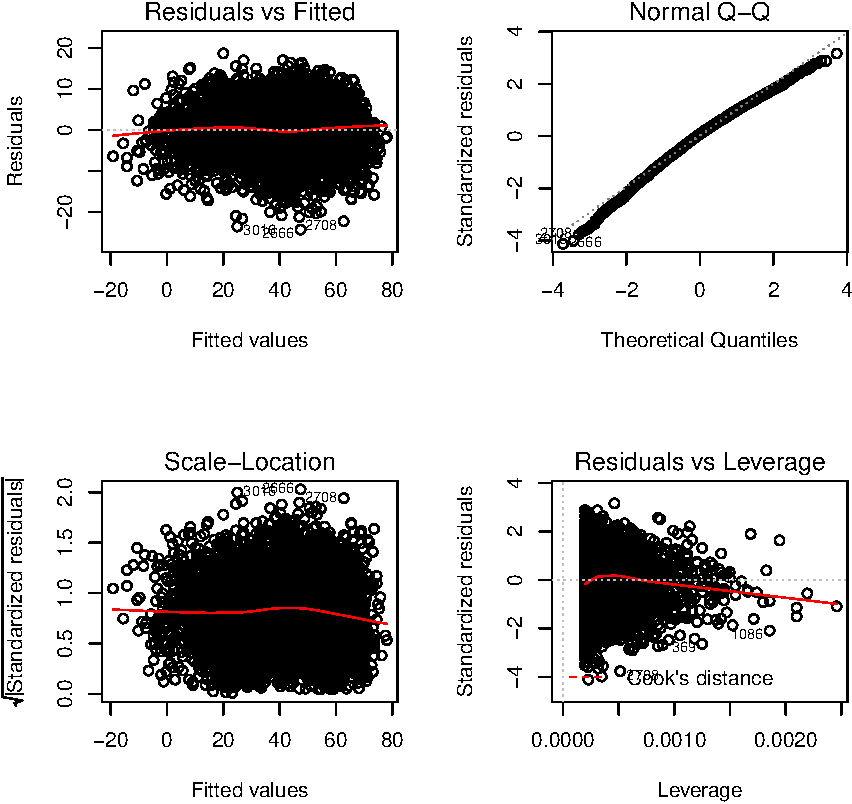
\includegraphics{RProgrammingForResearch_files/figure-latex/unnamed-chunk-213-1.pdf}

\begin{Shaded}
\begin{Highlighting}[]
\KeywordTok{par}\NormalTok{(}\DataTypeTok{mfrow =} \KeywordTok{c}\NormalTok{(}\DecValTok{1}\NormalTok{, }\DecValTok{1}\NormalTok{)) }\CommentTok{# Reset to one plot per panel}
\end{Highlighting}
\end{Shaded}

Try fitting the model using \texttt{glm()}. Call it \texttt{mod\_1a}.
Compare the coefficients for the two models. You can use the
\texttt{coef()} function on an \texttt{lm} or \texttt{glm} object to
pull out just the model coefficients.

\begin{Shaded}
\begin{Highlighting}[]
\NormalTok{mod_1a <-}\StringTok{ }\KeywordTok{glm}\NormalTok{(dptp ~}\StringTok{ }\NormalTok{temp, }\DataTypeTok{data =} \NormalTok{chic)}

\KeywordTok{coef}\NormalTok{(mod_1)}
\end{Highlighting}
\end{Shaded}

\begin{verbatim}
## (Intercept)        temp 
##    24.02487     1.62065
\end{verbatim}

\begin{Shaded}
\begin{Highlighting}[]
\KeywordTok{coef}\NormalTok{(mod_1a)}
\end{Highlighting}
\end{Shaded}

\begin{verbatim}
## (Intercept)        temp 
##    24.02487     1.62065
\end{verbatim}

The results from the two models are identical.

Fit a model of \(PM_{10}\) regressed on day of week, where day of week
is a factor.

\begin{Shaded}
\begin{Highlighting}[]
\NormalTok{mod_2 <-}\StringTok{ }\KeywordTok{lm}\NormalTok{(pm10 ~}\StringTok{ }\NormalTok{dow, }\DataTypeTok{data =} \NormalTok{chic)}
\KeywordTok{summary}\NormalTok{(mod_2)}
\end{Highlighting}
\end{Shaded}

\begin{verbatim}
## 
## Call:
## lm(formula = pm10 ~ dow, data = chic)
## 
## Residuals:
##    Min     1Q Median     3Q    Max 
## -39.05 -12.55  -3.34   8.80 328.66 
## 
## Coefficients:
##              Estimate Std. Error t value Pr(>|t|)    
## (Intercept)   27.5217     0.7303  37.684  < 2e-16 ***
## dowMonday      6.1322     1.0340   5.931 3.22e-09 ***
## dowTuesday     6.7954     1.0269   6.617 4.05e-11 ***
## dowWednesday   8.4768     1.0262   8.261  < 2e-16 ***
## dowThursday    8.8047     1.0240   8.598  < 2e-16 ***
## dowFriday      9.4816     1.0262   9.240  < 2e-16 ***
## dowSaturday    3.6602     1.0269   3.564 0.000368 ***
## ---
## Signif. codes:  0 '***' 0.001 '**' 0.01 '*' 0.05 '.' 0.1 ' ' 1
## 
## Residual standard error: 19.07 on 4856 degrees of freedom
##   (251 observations deleted due to missingness)
## Multiple R-squared:  0.02588,    Adjusted R-squared:  0.02467 
## F-statistic:  21.5 on 6 and 4856 DF,  p-value: < 2.2e-16
\end{verbatim}

Use the \texttt{anova()} command to compare this model to a model with
only an intercept (i.e., one that only fits a global mean and uses that
as the expected value for all of the observations).

\begin{Shaded}
\begin{Highlighting}[]
\KeywordTok{anova}\NormalTok{(mod_2)}
\end{Highlighting}
\end{Shaded}

\begin{verbatim}
## Analysis of Variance Table
## 
## Response: pm10
##             Df  Sum Sq Mean Sq F value    Pr(>F)    
## dow          6   46924  7820.6    21.5 < 2.2e-16 ***
## Residuals 4856 1766407   363.8                      
## ---
## Signif. codes:  0 '***' 0.001 '**' 0.01 '*' 0.05 '.' 0.1 ' ' 1
\end{verbatim}

The p-value for an ANOVA of the model with day-of-week coefficients
versus the model that just has an intercept is \textless{} 2.2e-16. This
is well below 0.05, which suggests that day-of-week is associated with
PM10 concentration, as a model that includes day-of-week does a much
better job of explaining variation in PM10 than a model without it does.
(Note, too, that the F value and Pr(\textgreater{}F) for the
\texttt{anova()} call are identical to the F-statistic information given
in the \texttt{summary()} of the model object. This will always be true
when you're using \texttt{anova()} to compare a model to a model with
just an intercept.)

Use a boxplot to visually compare PM10 by day of week.

\begin{Shaded}
\begin{Highlighting}[]
\KeywordTok{ggplot}\NormalTok{(chic, }\KeywordTok{aes}\NormalTok{(}\DataTypeTok{x =} \NormalTok{dow, }\DataTypeTok{y =} \NormalTok{pm10)) +}\StringTok{ }
\StringTok{  }\KeywordTok{geom_boxplot}\NormalTok{()}
\end{Highlighting}
\end{Shaded}

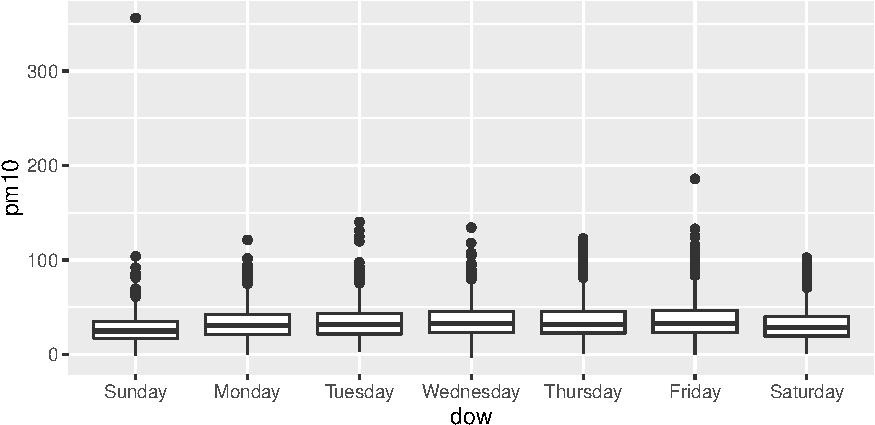
\includegraphics{RProgrammingForResearch_files/figure-latex/unnamed-chunk-217-1.pdf}

Now try the same plot, but try using the \texttt{ylim\ =} option to
change the limits on the y-axis for the graph, so you can get a better
idea of the pattern by day of week (some of the extreme values are very
high, which makes it hard to compare by eye when the y-axis extends to
include them all).

\begin{Shaded}
\begin{Highlighting}[]
\KeywordTok{ggplot}\NormalTok{(chic, }\KeywordTok{aes}\NormalTok{(}\DataTypeTok{x =} \NormalTok{dow, }\DataTypeTok{y =} \NormalTok{pm10)) +}\StringTok{ }
\StringTok{  }\KeywordTok{geom_boxplot}\NormalTok{() +}\StringTok{ }
\StringTok{  }\KeywordTok{ylim}\NormalTok{(}\KeywordTok{c}\NormalTok{(}\DecValTok{0}\NormalTok{, }\DecValTok{100}\NormalTok{))}
\end{Highlighting}
\end{Shaded}

\begin{verbatim}
## Warning: Removed 292 rows containing non-finite values (stat_boxplot).
\end{verbatim}

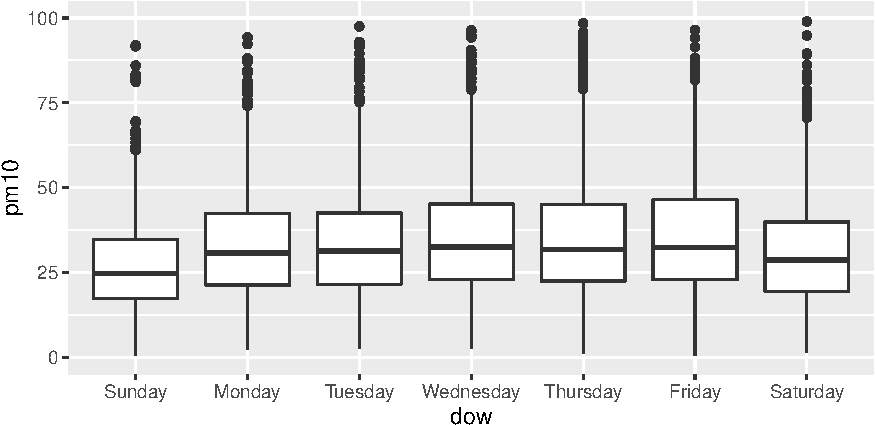
\includegraphics{RProgrammingForResearch_files/figure-latex/unnamed-chunk-218-1.pdf}

Create a subset called \texttt{summer} with just the summer days:

\begin{Shaded}
\begin{Highlighting}[]
\NormalTok{summer <-}\StringTok{ }\NormalTok{chic %>%}
\StringTok{  }\KeywordTok{filter}\NormalTok{(month %in%}\StringTok{ }\DecValTok{6}\NormalTok{:}\DecValTok{8}\NormalTok{)}
\end{Highlighting}
\end{Shaded}

Use \texttt{glm()} to fit a Poisson model of respiratory deaths
regressed on temperature. Since you want to fit a Poisson model, use the
option \texttt{family\ =\ poisson(link\ =\ "log")}.

\begin{Shaded}
\begin{Highlighting}[]
\NormalTok{mod_3 <-}\StringTok{ }\KeywordTok{glm}\NormalTok{(resp ~}\StringTok{ }\NormalTok{temp, }\DataTypeTok{data =} \NormalTok{summer,}
             \DataTypeTok{family =} \KeywordTok{poisson}\NormalTok{(}\DataTypeTok{link =} \StringTok{"log"}\NormalTok{))}
\KeywordTok{summary}\NormalTok{(mod_3)}
\end{Highlighting}
\end{Shaded}

\begin{verbatim}
## 
## Call:
## glm(formula = resp ~ temp, family = poisson(link = "log"), data = summer)
## 
## Deviance Residuals: 
##     Min       1Q   Median       3Q      Max  
## -3.9755  -0.7162  -0.1807   0.6927   3.6555  
## 
## Coefficients:
##             Estimate Std. Error z value Pr(>|z|)    
## (Intercept) 1.910317   0.058373  32.726   <2e-16 ***
## temp        0.006137   0.002581   2.378   0.0174 *  
## ---
## Signif. codes:  0 '***' 0.001 '**' 0.01 '*' 0.05 '.' 0.1 ' ' 1
## 
## (Dispersion parameter for poisson family taken to be 1)
## 
##     Null deviance: 1499.4  on 1287  degrees of freedom
## Residual deviance: 1493.8  on 1286  degrees of freedom
## AIC: 6425.4
## 
## Number of Fisher Scoring iterations: 4
\end{verbatim}

Use the fitted model coefficient to determine the relative risk for a
one degree Celcius increase in temperature. First, remember that you can
use the \texttt{coef()} function to read out the model coefficients. The
second of these is the value for the temperature coefficient. That means
that you can use indexing (\texttt{{[}2{]}}) to get just that value.
That's the log relative risk; take the exponent to get the relative
risk.

\begin{Shaded}
\begin{Highlighting}[]
\KeywordTok{coef}\NormalTok{(mod_3)}
\end{Highlighting}
\end{Shaded}

\begin{verbatim}
## (Intercept)        temp 
## 1.910316958 0.006136743
\end{verbatim}

\begin{Shaded}
\begin{Highlighting}[]
\KeywordTok{coef}\NormalTok{(mod_3)[}\DecValTok{2}\NormalTok{]}
\end{Highlighting}
\end{Shaded}

\begin{verbatim}
##        temp 
## 0.006136743
\end{verbatim}

\begin{Shaded}
\begin{Highlighting}[]
\KeywordTok{exp}\NormalTok{(}\KeywordTok{coef}\NormalTok{(mod_3)[}\DecValTok{2}\NormalTok{])}
\end{Highlighting}
\end{Shaded}

\begin{verbatim}
##     temp 
## 1.006156
\end{verbatim}

\chapter{Reporting data results \#1}\label{reporting-data-results-1}

\href{https://github.com/geanders/RProgrammingForResearch/raw/master/slides/CourseNotes_Week4.pdf}{Download}
a pdf of the lecture slides covering this topic.

\section{Guidelines for good plots}\label{guidelines-for-good-plots}

There are a number of very thoughtful books and articles about creating
graphics that effectively communicate information. \medskip

Some of the authors I highly recommend (and from whose work I've pulled
the guidelines for good graphics we'll talk about this week) are:

\begin{itemize}
\tightlist
\item
  Edward Tufte
\item
  Howard Wainer
\item
  Stephen Few
\item
  Nathan Yau
\end{itemize}

You should plan, in particular, to read \emph{The Visual Display of
Quantitative Information} by Edward Tufte before you graduate.

This week, we'll focus on six guidelines for good graphics, based on the
writings of these and other specialists in data display. \medskip

The guidelines are:

\begin{enumerate}
\def\labelenumi{\arabic{enumi}.}
\tightlist
\item
  Aim for high data density.
\item
  Use clear, meaningful labels.
\item
  Provide useful references.
\item
  Highlight interesting aspects of the data.
\item
  Make order meaningful.
\item
  When possible, use small multiples.
\end{enumerate}

For the examples, I'll use \texttt{dplyr} for data cleaning and, for
plotting, the packages \texttt{ggplot2}, \texttt{gridExtra}, and
\texttt{ggthemes}.

\begin{Shaded}
\begin{Highlighting}[]
\KeywordTok{library}\NormalTok{(dplyr)}

\KeywordTok{library}\NormalTok{(ggplot2)}
\KeywordTok{library}\NormalTok{(gridExtra)}
\KeywordTok{library}\NormalTok{(ggthemes)}
\end{Highlighting}
\end{Shaded}

You can load the data for today's examples with the following code:

\begin{Shaded}
\begin{Highlighting}[]
\KeywordTok{library}\NormalTok{(faraway)}
\KeywordTok{data}\NormalTok{(nepali)}
\KeywordTok{data}\NormalTok{(worldcup)}

\KeywordTok{library}\NormalTok{(dlnm)}
\KeywordTok{data}\NormalTok{(chicagoNMMAPS)}
\NormalTok{chic <-}\StringTok{ }\NormalTok{chicagoNMMAPS}
\NormalTok{chic_july <-}\StringTok{ }\NormalTok{chic %>%}
\StringTok{  }\KeywordTok{filter}\NormalTok{(month ==}\StringTok{ }\DecValTok{7} \NormalTok{&}\StringTok{ }\NormalTok{year ==}\StringTok{ }\DecValTok{1995}\NormalTok{)}
\end{Highlighting}
\end{Shaded}

\section{High data density}\label{high-data-density}

Guideline 1: \textbf{Aim for high data density.} \bigskip

You should try to increase, as much as possible, the \textbf{data to ink
ratio} in your graphs. This is the ratio of ``ink'' providing
information to all ink used in the figure. \medskip

One way to think about this is that the only graphs you make that use up
a lot of your printer's ink should be packed with information.

The two graphs below show the same information. Compare the amount of
ink used in the left plot to the amount used in the right plot to see
how graphs with the same information can have very different data
densities. \bigskip

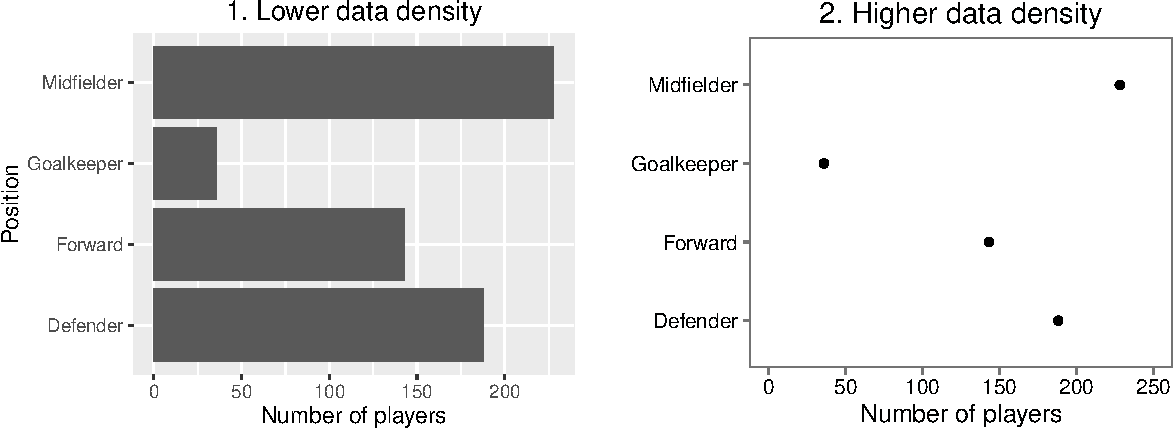
\includegraphics{RProgrammingForResearch_files/figure-latex/unnamed-chunk-224-1.pdf}

The two graphs below show another example of very different data
densities in two plots showing the same information: \bigskip

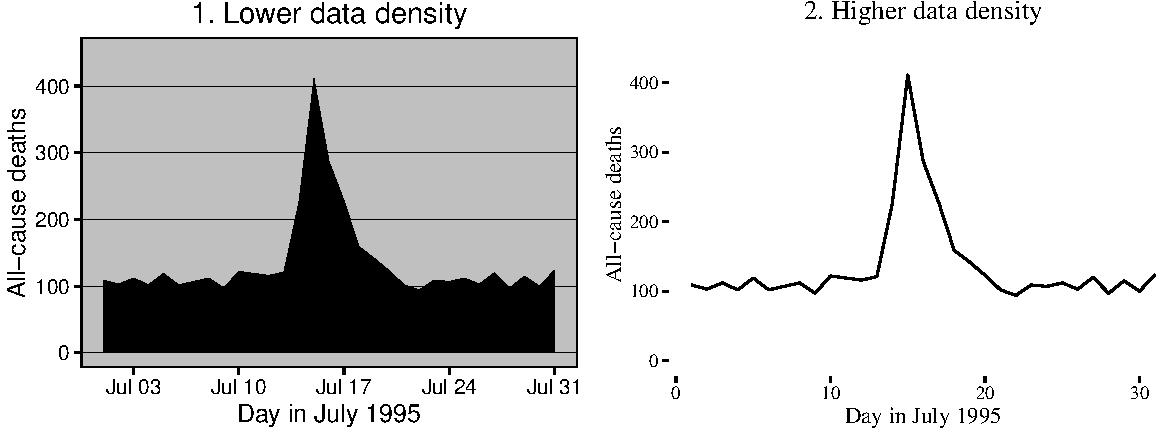
\includegraphics{RProgrammingForResearch_files/figure-latex/unnamed-chunk-225-1.pdf}

One quick way to increase data density in \texttt{ggplot2} is to change
the \emph{theme} for the plot. This essentially changes the
``background'' elements to a plot, including elements like the plot
grid, background color, and the font used for labeling. \bigskip

Some themes come with \texttt{ggplto2}, including:

\begin{itemize}
\tightlist
\item
  \texttt{theme\_bw}
\item
  \texttt{theme\_minimal}
\item
  \texttt{theme\_void}
\end{itemize}

The \texttt{ggthemes} packages has some excellent additional themes.

The following slides show some examples of the effects of using
different themes. The following code creates a plot of daily deaths in
Chicago in July 1995:

\begin{Shaded}
\begin{Highlighting}[]
\NormalTok{chic_plot <-}\StringTok{ }\KeywordTok{ggplot}\NormalTok{(chic_july, }\KeywordTok{aes}\NormalTok{(}\DataTypeTok{x =} \NormalTok{date, }\DataTypeTok{y =} \NormalTok{death))  +}
\StringTok{        }\KeywordTok{geom_point}\NormalTok{(}\DataTypeTok{color =} \StringTok{"red"}\NormalTok{)}
\end{Highlighting}
\end{Shaded}

Next, we can see how the graph looks with the default theme and with
other themes.

The left graph shows the graph with the default theme, while the right
shows the effect of adding the black-and-white theme that comes with
\texttt{ggplot2} as \texttt{theme\_bw}:

\begin{Shaded}
\begin{Highlighting}[]
\NormalTok{a <-}\StringTok{ }\NormalTok{chic_plot}
\NormalTok{b <-}\StringTok{ }\NormalTok{chic_plot +}\StringTok{ }\KeywordTok{theme_bw}\NormalTok{()}
\KeywordTok{grid.arrange}\NormalTok{(a, b, }\DataTypeTok{ncol =} \DecValTok{2}\NormalTok{)}
\end{Highlighting}
\end{Shaded}

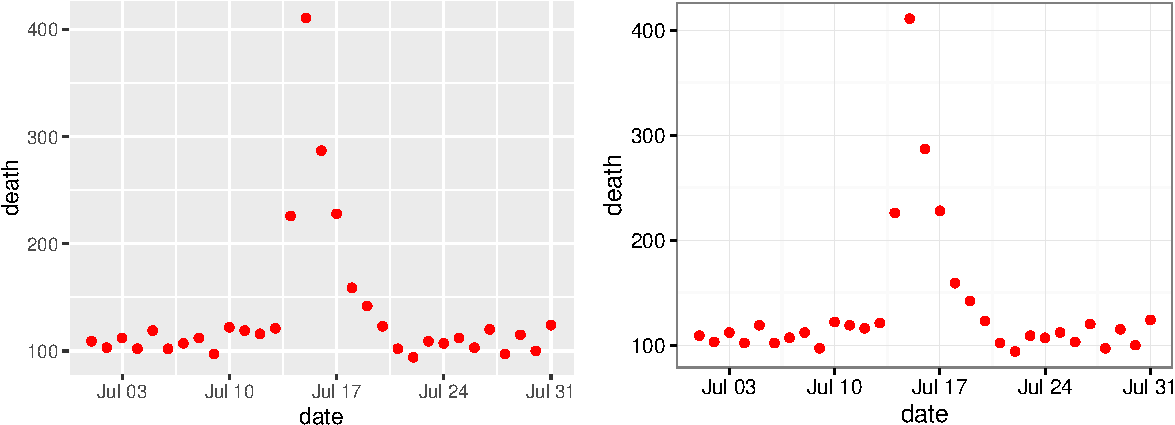
\includegraphics{RProgrammingForResearch_files/figure-latex/unnamed-chunk-227-1.pdf}

Stephen Few theme:

\begin{Shaded}
\begin{Highlighting}[]
\NormalTok{a <-}\StringTok{ }\NormalTok{chic_plot}
\NormalTok{b <-}\StringTok{ }\NormalTok{chic_plot +}\StringTok{ }\KeywordTok{theme_few}\NormalTok{()}
\KeywordTok{grid.arrange}\NormalTok{(a, b, }\DataTypeTok{ncol =} \DecValTok{2}\NormalTok{)}
\end{Highlighting}
\end{Shaded}

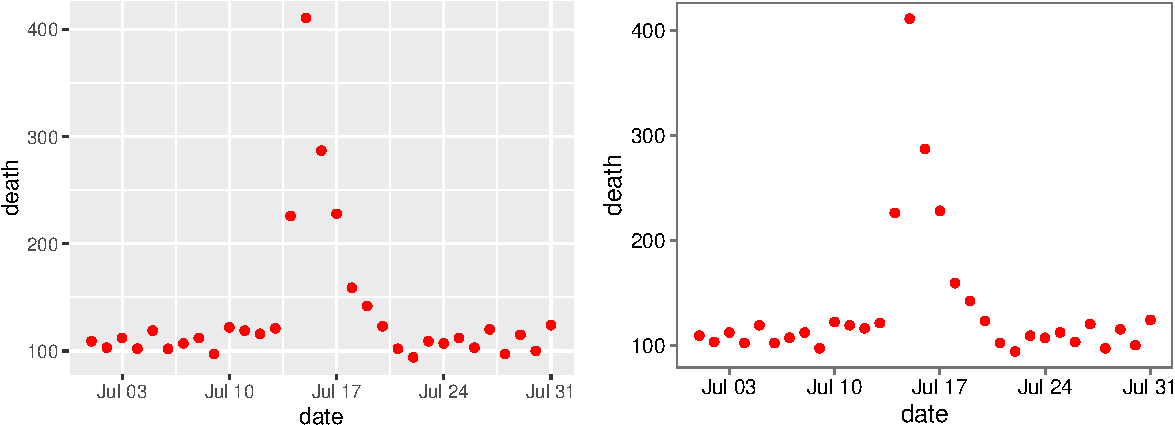
\includegraphics{RProgrammingForResearch_files/figure-latex/unnamed-chunk-228-1.pdf}

Edward Tufte theme:

\begin{Shaded}
\begin{Highlighting}[]
\NormalTok{a <-}\StringTok{ }\NormalTok{chic_plot}
\NormalTok{b <-}\StringTok{ }\NormalTok{chic_plot +}\StringTok{ }\KeywordTok{theme_tufte}\NormalTok{()}
\KeywordTok{grid.arrange}\NormalTok{(a, b, }\DataTypeTok{ncol =} \DecValTok{2}\NormalTok{)}
\end{Highlighting}
\end{Shaded}

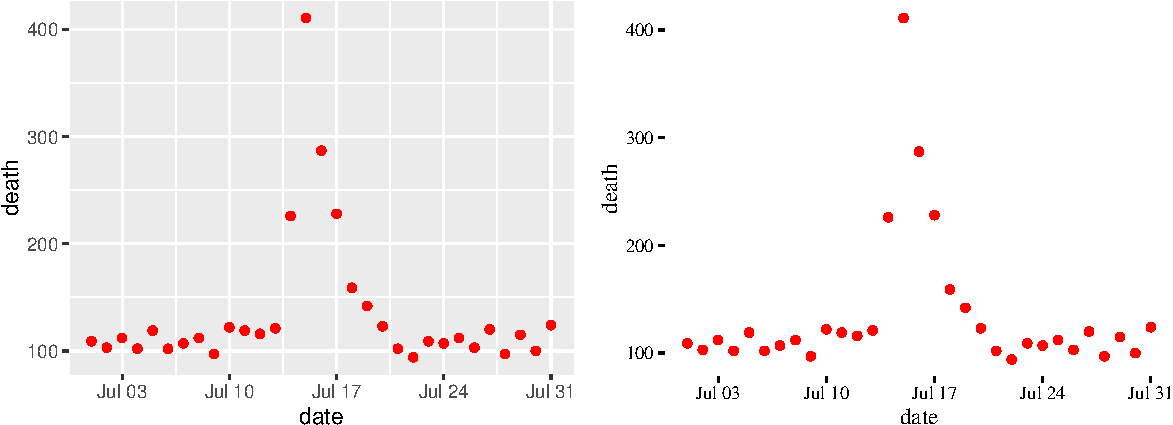
\includegraphics{RProgrammingForResearch_files/figure-latex/unnamed-chunk-229-1.pdf}

You can even use themes to add some questionable choices for different
elements. For example, \texttt{ggthemes} includes an Excel theme:

\begin{Shaded}
\begin{Highlighting}[]
\NormalTok{a <-}\StringTok{ }\NormalTok{chic_plot}
\NormalTok{b <-}\StringTok{ }\NormalTok{chic_plot +}\StringTok{ }\KeywordTok{theme_excel}\NormalTok{()}
\KeywordTok{grid.arrange}\NormalTok{(a, b, }\DataTypeTok{ncol =} \DecValTok{2}\NormalTok{)}
\end{Highlighting}
\end{Shaded}

\includegraphics{RProgrammingForResearch_files/figure-latex/unnamed-chunk-230-1.pdf}

\section{Meaningful labels}\label{meaningful-labels}

Guideline 2: \textbf{Use clear, meaningful labels.} \bigskip

Graph defaults often use abbreviations for axis labels and other
labeling. Furthermore, text labels can sometimes be aligned in a way
that makes them hard to read. The plots below give an example of the
same information shown without (left) and with (right) clear, meaningful
labels. \bigskip

\includegraphics{RProgrammingForResearch_files/figure-latex/unnamed-chunk-231-1.pdf}

There are a few strategies you can use to make labels clearer:

\begin{itemize}
\tightlist
\item
  Add \texttt{xlab} and \texttt{ylab} elements to the plot, rather than
  relying on the column names in the original data. This can also be
  done with \texttt{scale} elements (e.g.,
  \texttt{scale\_x\_continuous}), which give you more power to also make
  other changes to the x- and y-axes.
\item
  Include units of measurement in axis titles when relevant. If units
  are dollars or percent, check out the \texttt{scales} package, which
  allows you to add labels directly to axis elements by including
  arguments like \texttt{labels\ =\ percent} in \texttt{scale} elements.
\item
  If the x-variable requires longer labels (player positions in the
  example above), consider flipping the coordinates, rather than
  abbreviating or rotating the labels. You can use \texttt{coord\_flip}
  to do this.
\end{itemize}

\section{References}\label{references}

Guideline 3: \textbf{Provide useful references.} \bigskip

Data is easier to interpret when you add references. For example, if you
show what it typical, it helps viewers interpret how unusual outliers
are. The graph below on the right has added shading showing the range of
daily deaths in July in Chicage for 1990--1994 and 1996--2000, to
clarify how unusual July 1995 was. \bigskip

\includegraphics{RProgrammingForResearch_files/figure-latex/unnamed-chunk-232-1.pdf}

Another useful way to add references is to add a linear or smooth fit to
the data, to help clarify trends in the data. \bigskip

\includegraphics{RProgrammingForResearch_files/figure-latex/unnamed-chunk-233-1.pdf}

You can use the function \texttt{geom\_smooth} to add a smooth or linear
reference line:

\begin{Shaded}
\begin{Highlighting}[]
\KeywordTok{ggplot}\NormalTok{(worldcup, }\KeywordTok{aes}\NormalTok{(}\DataTypeTok{x =} \NormalTok{Passes, }\DataTypeTok{y =} \NormalTok{Shots)) +}\StringTok{ }
\StringTok{  }\KeywordTok{geom_point}\NormalTok{() +}\StringTok{ }\KeywordTok{theme_few}\NormalTok{() +}\StringTok{ }
\StringTok{  }\KeywordTok{geom_smooth}\NormalTok{(}\DataTypeTok{method =} \StringTok{"lm"}\NormalTok{)}
\end{Highlighting}
\end{Shaded}

\begin{center}\includegraphics[width=0.4\textwidth]{RProgrammingForResearch_files/figure-latex/unnamed-chunk-234-1} \end{center}

The most useful \texttt{geom\_smooth} parameters to know are:

\begin{itemize}
\tightlist
\item
  \texttt{method}: The default is to add a loess curve if the data
  includes less than 1000 points and a generalized additive model for
  1000 points or more. However, you can change to show the fitted line
  from a linear model using \texttt{method\ =\ "lm"} or from a
  generalized linear model using \texttt{method\ =\ "glm"}.
\item
  \texttt{span}: How wiggly or smooth the smooth line should be (smaller
  value: more wiggly; larger value: more smooth)
\item
  \texttt{se}: TRUE or FALSE, indicating whether to include shading for
  95\% confidence intervals.
\item
  \texttt{level}: Confidence level for confidence interval (e.g.,
  \texttt{0.90} for 90\% confidence intervals)
\end{itemize}

Lines and polygons can also be useful for adding references. Useful
geoms include:

\begin{itemize}
\tightlist
\item
  \texttt{geom\_hline}, \texttt{geom\_vline}: Add a horizontal or
  vertical line
\item
  \texttt{geom\_abline}: Add a line with an intercept and slope
\item
  \texttt{geom\_polygon}: Add a filled polygon
\item
  \texttt{geom\_path}: Add an unfilled polygon
\end{itemize}

When adding these references:

\begin{itemize}
\tightlist
\item
  Add reference elements first, so they will be plotted under the data,
  instead of on top of it.
\item
  Use \texttt{alpha} to add transparency to these elements.
\item
  Use colors that are unobtrusive (e.g., grays)
\item
  For lines, consider using non-solid line types (e.g.,
  \texttt{linetype\ =\ 3})
\end{itemize}

\section{Highlighting}\label{highlighting}

Guideline 3: \textbf{Highlight interesting aspects.} \bigskip

Consider adding elements to highlight noteworthy elements of the data.
For example, in the graph on the right, the days of a major heat wave
have been highlighted with a red line. \bigskip

\includegraphics{RProgrammingForResearch_files/figure-latex/unnamed-chunk-235-1.pdf}

In the below graphs, the names of the players with the most shots and
passes have been added to highlight these unusual points. \bigskip

\includegraphics{RProgrammingForResearch_files/figure-latex/unnamed-chunk-236-1.pdf}

One helpful way to annotate is with text, using \texttt{geom\_text()}.
For this, you'll first need to create a dataframe with the hottest day
in the data:

\begin{Shaded}
\begin{Highlighting}[]
\NormalTok{hottest_day <-}\StringTok{ }\NormalTok{chic_july %>%}
\StringTok{  }\KeywordTok{filter}\NormalTok{(temp ==}\StringTok{ }\KeywordTok{max}\NormalTok{(temp))}
\NormalTok{hottest_day[ , }\DecValTok{1}\NormalTok{:}\DecValTok{6}\NormalTok{]}
\end{Highlighting}
\end{Shaded}

\begin{verbatim}
##         date time year month doy      dow
## 1 1995-07-13 3116 1995     7 194 Thursday
\end{verbatim}

\begin{Shaded}
\begin{Highlighting}[]
\NormalTok{chic_plot +}\StringTok{ }\KeywordTok{geom_text}\NormalTok{(}\DataTypeTok{data =} \NormalTok{hottest_day, }
                      \DataTypeTok{label =} \StringTok{"Max"}\NormalTok{,}
                      \DataTypeTok{size =} \DecValTok{3}\NormalTok{)}
\end{Highlighting}
\end{Shaded}

\begin{center}\includegraphics[width=0.7\textwidth]{RProgrammingForResearch_files/figure-latex/unnamed-chunk-238-1} \end{center}

With \texttt{geom\_text}, you'll often want to use position adjustment
(the \texttt{position} parameter) to move the text so it won't be right
on top of the data points:

\begin{Shaded}
\begin{Highlighting}[]
\NormalTok{chic_plot +}\StringTok{ }\KeywordTok{geom_text}\NormalTok{(}\DataTypeTok{data =} \NormalTok{hottest_day, }
                      \DataTypeTok{label =} \StringTok{"Max"}\NormalTok{,}
                      \DataTypeTok{size =} \DecValTok{3}\NormalTok{, }\DataTypeTok{hjust =} \DecValTok{0}\NormalTok{, }\DataTypeTok{vjust =} \NormalTok{-}\DecValTok{1}\NormalTok{)}
\end{Highlighting}
\end{Shaded}

\begin{center}\includegraphics[width=0.5\textwidth]{RProgrammingForResearch_files/figure-latex/unnamed-chunk-239-1} \end{center}

You can also use lines to highlight. For this, it is often useful to
create a new dataframe with data for the reference. To add a line for
the Chicago heat wave, I've added a dataframe called \texttt{hw} with
the relevant date range. I'm setting the y-value to be high enough (425)
to ensure the line will be placed above the mortality data.

\begin{Shaded}
\begin{Highlighting}[]
\NormalTok{hw <-}\StringTok{ }\KeywordTok{data.frame}\NormalTok{(}\DataTypeTok{date =} \KeywordTok{c}\NormalTok{(}\KeywordTok{as.Date}\NormalTok{(}\StringTok{"1995-07-12"}\NormalTok{), }
                          \KeywordTok{as.Date}\NormalTok{(}\StringTok{"1995-07-16"}\NormalTok{)),}
                 \DataTypeTok{death =} \KeywordTok{c}\NormalTok{(}\DecValTok{425}\NormalTok{, }\DecValTok{425}\NormalTok{))}
        
\NormalTok{b <-}\StringTok{ }\NormalTok{chic_plot +}\StringTok{ }
\StringTok{        }\KeywordTok{geom_line}\NormalTok{(}\DataTypeTok{data =} \NormalTok{hw,}
                  \KeywordTok{aes}\NormalTok{(}\DataTypeTok{x =} \NormalTok{date, }\DataTypeTok{y =} \NormalTok{death),}
                  \DataTypeTok{size =} \DecValTok{2}\NormalTok{)}
\end{Highlighting}
\end{Shaded}

\begin{Shaded}
\begin{Highlighting}[]
\NormalTok{b}
\end{Highlighting}
\end{Shaded}

\begin{center}\includegraphics[width=0.7\textwidth]{RProgrammingForResearch_files/figure-latex/unnamed-chunk-241-1} \end{center}

\section{Order}\label{order}

Guideline 4: \textbf{Make order meaningful.} \bigskip

You can make the ranking of data clearer from a graph by using order to
show rank. Often, factor or categorical variables are ordered by
something that is not interesting, like alphabetical order.

\includegraphics{RProgrammingForResearch_files/figure-latex/unnamed-chunk-242-1.pdf}

You can re-order factor variables in a graph by resetting the factor
using the \texttt{factor} function and changing the order that levels
are included in the \texttt{levels} parameter.

\section{Small multiples}\label{small-multiples}

Guideline 5: \textbf{When possible, use small multiples.} \bigskip

\emph{Small multiples} are graphs that use many small plots showing the
same thing for different facets of the data. For example, instead of
using color in a single plot to show data for males and females, you
could use two small plots, one each for males and females. \bigskip

Typically, in small multiples, all plots use the same x- and y-axes.
This makes it easier to compare across plots, and it also allows you to
save room by limiting axis annotation.

\includegraphics{RProgrammingForResearch_files/figure-latex/unnamed-chunk-243-1.pdf}

You can use the \texttt{facet} functions to create small multiples. This
separates the graph into several small graphs, one for each level of a
factor. \bigskip

The \texttt{facet} functions are:

\begin{itemize}
\tightlist
\item
  \texttt{facet\_grid()}
\item
  \texttt{facet\_wrap()}
\end{itemize}

For example, to create small multiples by sex for the Nepali dataset,
when plotting height versus weight, you can call:

\begin{Shaded}
\begin{Highlighting}[]
\KeywordTok{ggplot}\NormalTok{(nepali, }\KeywordTok{aes}\NormalTok{(ht, wt)) +}\StringTok{ }
\StringTok{        }\KeywordTok{geom_point}\NormalTok{() +}\StringTok{ }
\StringTok{        }\KeywordTok{facet_grid}\NormalTok{(. ~}\StringTok{ }\NormalTok{sex)}
\end{Highlighting}
\end{Shaded}

\includegraphics{RProgrammingForResearch_files/figure-latex/unnamed-chunk-244-1.pdf}

The \texttt{facet\_grid} function can facet by one or two variables. One
will be shown by rows, and one by columns:

\begin{Shaded}
\begin{Highlighting}[]
\NormalTok{## Generic code}
\KeywordTok{facet_grid}\NormalTok{([factor for rows] ~}\StringTok{ }\NormalTok{[factor for columns])}
\end{Highlighting}
\end{Shaded}

The \texttt{facet\_wrap()} function can only facet by one variable, but
it can ``wrap'' the small graphs for that variable, so the don't all
have to be in one row or column:

\begin{Shaded}
\begin{Highlighting}[]
\NormalTok{## Generic code}
\KeywordTok{facet_wrap}\NormalTok{(~}\StringTok{ }\NormalTok{[factor for faceting], }\DataTypeTok{ncol =} \NormalTok{[number of columns])}
\end{Highlighting}
\end{Shaded}

Often, when you do faceting, you'll want to re-name your factors levels
or re-order them. For this, you'll need to use the \texttt{factor()}
function on the original vector. For example, to rename the \texttt{sex}
factor levels from ``1'' and ``2'' to ``Male'' and ``Female'', you can
run:

\begin{Shaded}
\begin{Highlighting}[]
\NormalTok{nepali <-}\StringTok{ }\NormalTok{nepali %>%}
\StringTok{  }\KeywordTok{mutate}\NormalTok{(}\DataTypeTok{sex =} \KeywordTok{factor}\NormalTok{(sex, }\DataTypeTok{levels =} \KeywordTok{c}\NormalTok{(}\DecValTok{1}\NormalTok{, }\DecValTok{2}\NormalTok{), }
                      \DataTypeTok{labels =} \KeywordTok{c}\NormalTok{(}\StringTok{"Male"}\NormalTok{, }\StringTok{"Female"}\NormalTok{)))}
\end{Highlighting}
\end{Shaded}

Notice that the labels for the two graphs have now changed:

\begin{Shaded}
\begin{Highlighting}[]
\KeywordTok{ggplot}\NormalTok{(nepali, }\KeywordTok{aes}\NormalTok{(ht, wt)) +}\StringTok{ }
\StringTok{        }\KeywordTok{geom_point}\NormalTok{() +}\StringTok{ }
\StringTok{        }\KeywordTok{facet_grid}\NormalTok{(. ~}\StringTok{ }\NormalTok{sex)}
\end{Highlighting}
\end{Shaded}

\includegraphics{RProgrammingForResearch_files/figure-latex/unnamed-chunk-248-1.pdf}

To re-order the factor, and show the plot for ``Female'' first, you can
use \texttt{factor} to change the order of the levels:

\begin{Shaded}
\begin{Highlighting}[]
\NormalTok{nepali <-}\StringTok{ }\NormalTok{nepali %>%}
\StringTok{  }\KeywordTok{mutate}\NormalTok{(}\DataTypeTok{sex =} \KeywordTok{factor}\NormalTok{(sex, }\DataTypeTok{levels =} \KeywordTok{c}\NormalTok{(}\StringTok{"Female"}\NormalTok{, }\StringTok{"Male"}\NormalTok{)))}
\end{Highlighting}
\end{Shaded}

Now notice that the order of the plots has changed:

\begin{Shaded}
\begin{Highlighting}[]
\KeywordTok{ggplot}\NormalTok{(nepali, }\KeywordTok{aes}\NormalTok{(ht, wt)) +}\StringTok{ }
\StringTok{        }\KeywordTok{geom_point}\NormalTok{() +}\StringTok{ }
\StringTok{        }\KeywordTok{facet_grid}\NormalTok{(. ~}\StringTok{ }\NormalTok{sex)}
\end{Highlighting}
\end{Shaded}

\includegraphics{RProgrammingForResearch_files/figure-latex/unnamed-chunk-250-1.pdf}

\section{Advanced customization}\label{advanced-customization}

\subsection{Scales}\label{scales}

There are a number of different functions for adjusting scales. These
follow the following convention:

\begin{Shaded}
\begin{Highlighting}[]
\NormalTok{## Generic code}
\NormalTok{scale_[aesthetic]_[vector type]}
\end{Highlighting}
\end{Shaded}

For example, to adjust the x-axis scale for a continuous variable, you'd
use \texttt{scale\_x\_continuous}. You can use a \texttt{scale} function
for an axis to change things like the axis label (which you could also
change with \texttt{xlab} or \texttt{ylab}) as well as position and
labeling of breaks.

For example, here is the default for plotting time versus passes for the
\texttt{worldcup} dataset, with the number of shots taken shown by size
and position shown by color:

\begin{Shaded}
\begin{Highlighting}[]
\KeywordTok{ggplot}\NormalTok{(worldcup, }\KeywordTok{aes}\NormalTok{(}\DataTypeTok{x =} \NormalTok{Time, }\DataTypeTok{y =} \NormalTok{Passes,}
                     \DataTypeTok{color =} \NormalTok{Position, }\DataTypeTok{size =} \NormalTok{Shots)) +}\StringTok{ }
\StringTok{  }\KeywordTok{geom_point}\NormalTok{(}\DataTypeTok{alpha =} \FloatTok{0.5}\NormalTok{)}
\end{Highlighting}
\end{Shaded}

\begin{center}\includegraphics[width=0.8\textwidth]{RProgrammingForResearch_files/figure-latex/unnamed-chunk-252-1} \end{center}

\begin{Shaded}
\begin{Highlighting}[]
\KeywordTok{ggplot}\NormalTok{(worldcup, }\KeywordTok{aes}\NormalTok{(}\DataTypeTok{x =} \NormalTok{Time, }\DataTypeTok{y =} \NormalTok{Passes,}
                     \DataTypeTok{color =} \NormalTok{Position, }\DataTypeTok{size =} \NormalTok{Shots)) +}\StringTok{ }
\StringTok{  }\KeywordTok{geom_point}\NormalTok{(}\DataTypeTok{alpha =} \FloatTok{0.5}\NormalTok{) +}\StringTok{ }
\StringTok{  }\KeywordTok{scale_x_continuous}\NormalTok{(}\DataTypeTok{name =} \StringTok{"Time played (minutes)"}\NormalTok{, }
                     \DataTypeTok{breaks =} \DecValTok{90} \NormalTok{*}\StringTok{ }\KeywordTok{c}\NormalTok{(}\DecValTok{2}\NormalTok{, }\DecValTok{4}\NormalTok{, }\DecValTok{6}\NormalTok{),}
                     \DataTypeTok{minor_breaks =} \DecValTok{90} \NormalTok{*}\StringTok{ }\KeywordTok{c}\NormalTok{(}\DecValTok{1}\NormalTok{, }\DecValTok{3}\NormalTok{, }\DecValTok{5}\NormalTok{))}
\end{Highlighting}
\end{Shaded}

\begin{center}\includegraphics[width=0.8\textwidth]{RProgrammingForResearch_files/figure-latex/unnamed-chunk-253-1} \end{center}

Parameters you might find useful in \texttt{scale} functions include:

\begin{tabular}{l|l}
\hline
Parameter & Description\\
\hline
name & Label or legend name\\
\hline
breaks & Vector of break points\\
\hline
minor\_breaks & Vector of minor break points\\
\hline
labels & Labels to use for each break\\
\hline
limits & Limits to the range of the axis\\
\hline
\end{tabular}

For dates, you can use \texttt{scale} functions like
\texttt{scale\_x\_date} and \texttt{scale\_x\_datetime}. For example,
here's a plot of deaths in Chicago in July 1995 using default values for
the x-axis:

\begin{Shaded}
\begin{Highlighting}[]
\KeywordTok{ggplot}\NormalTok{(chic_july, }\KeywordTok{aes}\NormalTok{(}\DataTypeTok{x =} \NormalTok{date, }\DataTypeTok{y =} \NormalTok{death)) +}\StringTok{ }
\StringTok{  }\KeywordTok{geom_line}\NormalTok{() }
\end{Highlighting}
\end{Shaded}

\begin{center}\includegraphics[width=0.9\textwidth]{RProgrammingForResearch_files/figure-latex/unnamed-chunk-255-1} \end{center}

And here's an example of changing the formating and name of the x-axis:

\begin{Shaded}
\begin{Highlighting}[]
\KeywordTok{ggplot}\NormalTok{(chic_july, }\KeywordTok{aes}\NormalTok{(}\DataTypeTok{x =} \NormalTok{date, }\DataTypeTok{y =} \NormalTok{death)) +}\StringTok{ }
\StringTok{  }\KeywordTok{geom_line}\NormalTok{() +}\StringTok{ }
\StringTok{  }\KeywordTok{scale_x_date}\NormalTok{(}\DataTypeTok{name =} \StringTok{"Date in July 1995"}\NormalTok{,}
               \DataTypeTok{date_labels =} \StringTok{"%m-%d"}\NormalTok{)}
\end{Highlighting}
\end{Shaded}

\begin{center}\includegraphics[width=0.9\textwidth]{RProgrammingForResearch_files/figure-latex/unnamed-chunk-256-1} \end{center}

You can also use the \texttt{scale} functions to transform an axis. For
example, to show the Chicago plot with ``deaths'' on a log scale, you
can run:

\begin{Shaded}
\begin{Highlighting}[]
\KeywordTok{ggplot}\NormalTok{(chic_july, }\KeywordTok{aes}\NormalTok{(}\DataTypeTok{x =} \NormalTok{date, }\DataTypeTok{y =} \NormalTok{death)) +}\StringTok{ }
\StringTok{  }\KeywordTok{geom_line}\NormalTok{() +}
\StringTok{  }\KeywordTok{scale_y_log10}\NormalTok{()}
\end{Highlighting}
\end{Shaded}

\begin{center}\includegraphics[width=0.9\textwidth]{RProgrammingForResearch_files/figure-latex/unnamed-chunk-257-1} \end{center}

For colors and fills, the conventions for the names of the
\texttt{scale} functions can vary. For example, to adjust the color
scale when you're mapping a discrete variable (i.e., categorical, like
gender or animal breed) to color, you'd use \texttt{scale\_color\_hue}.
To adjust the color scale for a continuous variable, like age, you'll
use \texttt{scale\_color\_gradient}.

For any color scales, consider starting with \texttt{brewer} first
(e.g., \texttt{scale\_color\_brewer}, \texttt{scale\_color\_distiller}).
Scale functions from \texttt{brewer} allow you to set colors using
different palettes. You can explore these palettes at
\url{http://colorbrewer2.org/}.

The Brewer palettes fall into three categories: sequential, divergent,
and qualitative. You should use sequential or divergent for continuous
data and qualitative for categorical data. Use
\texttt{display.brewer.pal} to show the palette for a given number of
colors.

\begin{Shaded}
\begin{Highlighting}[]
\KeywordTok{library}\NormalTok{(RColorBrewer)}
\KeywordTok{display.brewer.pal}\NormalTok{(}\DataTypeTok{name =} \StringTok{"Set1"}\NormalTok{, }\DataTypeTok{n =} \DecValTok{8}\NormalTok{)}
\KeywordTok{display.brewer.pal}\NormalTok{(}\DataTypeTok{name =} \StringTok{"PRGn"}\NormalTok{, }\DataTypeTok{n =} \DecValTok{8}\NormalTok{)}
\KeywordTok{display.brewer.pal}\NormalTok{(}\DataTypeTok{name =} \StringTok{"PuBuGn"}\NormalTok{, }\DataTypeTok{n =} \DecValTok{8}\NormalTok{)}
\end{Highlighting}
\end{Shaded}

\includegraphics[width=0.32\textwidth]{RProgrammingForResearch_files/figure-latex/unnamed-chunk-258-1}
\includegraphics[width=0.32\textwidth]{RProgrammingForResearch_files/figure-latex/unnamed-chunk-258-2}
\includegraphics[width=0.32\textwidth]{RProgrammingForResearch_files/figure-latex/unnamed-chunk-258-3}

Use the \texttt{palette} argument within a \texttt{scales} function to
customize the palette:

\begin{Shaded}
\begin{Highlighting}[]
\NormalTok{a <-}\StringTok{ }\KeywordTok{ggplot}\NormalTok{(}\KeywordTok{data.frame}\NormalTok{(}\DataTypeTok{x =} \DecValTok{1}\NormalTok{:}\DecValTok{5}\NormalTok{, }\DataTypeTok{y =} \KeywordTok{rnorm}\NormalTok{(}\DecValTok{5}\NormalTok{),}
                       \DataTypeTok{group =} \NormalTok{letters[}\DecValTok{1}\NormalTok{:}\DecValTok{5}\NormalTok{]),}
            \KeywordTok{aes}\NormalTok{(}\DataTypeTok{x =} \NormalTok{x, }\DataTypeTok{y =} \NormalTok{y, }\DataTypeTok{color =} \NormalTok{group)) +}\StringTok{ }
\StringTok{  }\KeywordTok{geom_point}\NormalTok{()}
\NormalTok{b <-}\StringTok{ }\NormalTok{a +}\StringTok{ }\KeywordTok{scale_color_brewer}\NormalTok{(}\DataTypeTok{palette =} \StringTok{"Set1"}\NormalTok{)}
\NormalTok{c <-}\StringTok{ }\NormalTok{a +}\StringTok{ }\KeywordTok{scale_color_brewer}\NormalTok{(}\DataTypeTok{palette =} \StringTok{"Pastel2"}\NormalTok{) +}\StringTok{ }
\StringTok{  }\KeywordTok{theme_dark}\NormalTok{()}
\KeywordTok{grid.arrange}\NormalTok{(a, b, c, }\DataTypeTok{ncol =} \DecValTok{3}\NormalTok{)}
\end{Highlighting}
\end{Shaded}

\includegraphics[width=\textwidth]{RProgrammingForResearch_files/figure-latex/unnamed-chunk-259-1}

\begin{Shaded}
\begin{Highlighting}[]
\KeywordTok{ggplot}\NormalTok{(worldcup, }\KeywordTok{aes}\NormalTok{(}\DataTypeTok{x =} \NormalTok{Time, }\DataTypeTok{y =} \NormalTok{Passes,}
                     \DataTypeTok{color =} \NormalTok{Position, }\DataTypeTok{size =} \NormalTok{Shots)) +}\StringTok{ }
\StringTok{  }\KeywordTok{geom_point}\NormalTok{(}\DataTypeTok{alpha =} \FloatTok{0.5}\NormalTok{) +}\StringTok{ }
\StringTok{  }\KeywordTok{scale_color_brewer}\NormalTok{(}\DataTypeTok{palette =} \StringTok{"Dark2"}\NormalTok{,}
                     \DataTypeTok{name =} \StringTok{"Player position"}\NormalTok{)}
\end{Highlighting}
\end{Shaded}

\begin{center}\includegraphics[width=0.8\textwidth]{RProgrammingForResearch_files/figure-latex/unnamed-chunk-260-1} \end{center}

You can also set colors manually:

\begin{Shaded}
\begin{Highlighting}[]
\KeywordTok{ggplot}\NormalTok{(worldcup, }\KeywordTok{aes}\NormalTok{(}\DataTypeTok{x =} \NormalTok{Time, }\DataTypeTok{y =} \NormalTok{Passes,}
                     \DataTypeTok{color =} \NormalTok{Position, }\DataTypeTok{size =} \NormalTok{Shots)) +}\StringTok{ }
\StringTok{  }\KeywordTok{geom_point}\NormalTok{(}\DataTypeTok{alpha =} \FloatTok{0.5}\NormalTok{) +}\StringTok{ }
\StringTok{  }\KeywordTok{scale_color_manual}\NormalTok{(}\DataTypeTok{values =} \KeywordTok{c}\NormalTok{(}\StringTok{"blue"}\NormalTok{, }\StringTok{"red"}\NormalTok{, }
                                \StringTok{"darkgreen"}\NormalTok{, }\StringTok{"darkgray"}\NormalTok{))}
\end{Highlighting}
\end{Shaded}

\begin{center}\includegraphics[width=0.8\textwidth]{RProgrammingForResearch_files/figure-latex/unnamed-chunk-261-1} \end{center}

\section{To find out more}\label{to-find-out-more}

Some excellent further references for plotting are:

\begin{itemize}
\tightlist
\item
  R Graphics Cookbook (book and website)
\item
  Google images
\end{itemize}

For more technical details about plotting in R:

\begin{itemize}
\tightlist
\item
  ggplot2: Elegant Graphics for Data Analysis, Hadley Wickham
\item
  R Graphics, Paul Murrell
\end{itemize}

\section{In-course exercise}\label{in-course-exercise-3}

\subsection{Designing a plot}\label{designing-a-plot}

For today's exercise, you'll be building a plot using the
\texttt{worldcup} data from the \texttt{faraway} package. First, load in
that data.

Next, say you want to look at the relationship between the number of
minutes that a player played in the 2010 World Cup (\texttt{Time}) and
the number of shots the player took on goal (\texttt{Shots}). On a sheet
of paper, and talking with your partner, decide how the two of you would
design a plot to explore and present this relationship. How would you
incorporate some of the principles of creating good graphs?

\subsubsection{Example R code}\label{example-r-code-4}

\begin{Shaded}
\begin{Highlighting}[]
\KeywordTok{library}\NormalTok{(faraway)}
\KeywordTok{data}\NormalTok{(worldcup)}
\KeywordTok{head}\NormalTok{(worldcup, }\DecValTok{2}\NormalTok{)}
\end{Highlighting}
\end{Shaded}

\begin{verbatim}
##           Team   Position Time Shots Passes Tackles Saves
## Abdoun Algeria Midfielder   16     0      6       0     0
## Abe      Japan Midfielder  351     0    101      14     0
\end{verbatim}

This dataset has the players' names as rownames, rather than in a
column. Once we start using \texttt{dplyr} functions, we'll lose these
rownames. Therefore, start by converting the rownames to a column called
\texttt{Player}:

\begin{Shaded}
\begin{Highlighting}[]
\KeywordTok{library}\NormalTok{(dplyr)}
\NormalTok{worldcup <-}\StringTok{ }\NormalTok{worldcup %>%}
\StringTok{  }\KeywordTok{mutate}\NormalTok{(}\DataTypeTok{Player =} \KeywordTok{rownames}\NormalTok{(worldcup))}
\KeywordTok{head}\NormalTok{(worldcup, }\DecValTok{2}\NormalTok{)}
\end{Highlighting}
\end{Shaded}

\begin{verbatim}
##      Team   Position Time Shots Passes Tackles Saves Player
## 1 Algeria Midfielder   16     0      6       0     0 Abdoun
## 2   Japan Midfielder  351     0    101      14     0    Abe
\end{verbatim}

\subsection{Basic scatterplots with R base graphics and
ggplot}\label{basic-scatterplots-with-r-base-graphics-and-ggplot}

Perform the following tasks:

\begin{itemize}
\tightlist
\item
  Install and load the \texttt{ggplot2} and \texttt{ggthemes} packages.
\item
  For the \texttt{worldcup} data, plot a scatterplot of Time (on the
  x-axis) versus Shots.
\item
  Add some ggplot elements to make this plot a bit more attractive. (For
  example, change the x- and y-axis labels and add a title.)
\end{itemize}

\subsubsection{Example R code}\label{example-r-code-5}

Install and load the \texttt{ggplot2} package:

\begin{Shaded}
\begin{Highlighting}[]
\CommentTok{# install.packages("ggplot2")}
\KeywordTok{library}\NormalTok{(ggplot2)}
\CommentTok{# install.packages("ggthemes")}
\KeywordTok{library}\NormalTok{(ggthemes)}
\end{Highlighting}
\end{Shaded}

Use the R base graphics to create a scatterplot of Time versus Shots:

\begin{Shaded}
\begin{Highlighting}[]
\KeywordTok{ggplot}\NormalTok{(worldcup, }\KeywordTok{aes}\NormalTok{(}\DataTypeTok{x =} \NormalTok{Time, }\DataTypeTok{y =} \NormalTok{Shots)) +}\StringTok{ }
\StringTok{        }\KeywordTok{geom_point}\NormalTok{()}
\end{Highlighting}
\end{Shaded}

\includegraphics{RProgrammingForResearch_files/figure-latex/unnamed-chunk-265-1.pdf}

Use some of the plotting options to improve the graph's appearance:

\begin{Shaded}
\begin{Highlighting}[]
\KeywordTok{ggplot}\NormalTok{(worldcup, }\KeywordTok{aes}\NormalTok{(}\DataTypeTok{x =} \NormalTok{Time, }\DataTypeTok{y =} \NormalTok{Shots)) +}\StringTok{ }
\StringTok{  }\KeywordTok{geom_point}\NormalTok{() +}\StringTok{ }
\StringTok{  }\KeywordTok{xlab}\NormalTok{(}\StringTok{"Minutes played"}\NormalTok{) +}\StringTok{ }
\StringTok{  }\KeywordTok{ylab}\NormalTok{(}\StringTok{"Shots on goal"}\NormalTok{) +}\StringTok{ }
\StringTok{  }\KeywordTok{ggtitle}\NormalTok{(}\StringTok{"Time played vs. shots taken}\CharTok{\textbackslash{}n}\StringTok{ World Cup 2010"}\NormalTok{)}
\end{Highlighting}
\end{Shaded}

\includegraphics{RProgrammingForResearch_files/figure-latex/unnamed-chunk-266-1.pdf}

\subsection{Fancier graphs}\label{fancier-graphs}

In this section, we'll work on creating a plot like this:

\includegraphics{RProgrammingForResearch_files/figure-latex/unnamed-chunk-267-1.pdf}

Try the following tasks:

\begin{itemize}
\tightlist
\item
  First, before you start coding, talk with your group members about how
  this graph is different from the simple one you created with
  \texttt{ggplot} in the last section. Also discuss what you can figure
  out from this new graph that was less clear from the simpler one you
  created before.
\item
  Use the \texttt{xlab()} function to make a clearer title for the
  x-axis. (You may have already written this code in the last section of
  this exercise.)
\item
  Often, in graphs with a lot of points, it's hard to see some of the
  points, because they overlap other points. Three strategies to address
  this are: (a) make the points smaller; (b) make the points somewhat
  transparent; and (c) jitter the points. Try doing the first two with
  the simple ggplot scatterplot you created in the previous section of
  Shots by Time.
\item
  Create a new column in the \texttt{worldcup} data called
  \texttt{top\_four} that specifies whether or not the \texttt{Team} for
  that observation was one of the top four teams in the tournament
  (Netherlands, Uruguay, Spain, and Germany). Make the colors of the
  points correspond to whether the team was a top-four team.
\item
  Create small multiples. The relationship between time played and shots
  taken is probably different by the players' positions. Use faceting to
  create different graphs for each position.
\item
  Make order count: What order are the faceted graphs currently in?
  Offensive players have more chances to take shots than defensive
  players, so that might be a useful ordering for the facets. Re-order
  the \texttt{Position} factor column to go from nearest your own goal
  to nearest the opponents goal, and then re-plot the graph from the
  previous step.
\item
  Highlighting interesting data: Who had the most shots in the 2010
  World Cup? Was he on a top-four team? Use \texttt{geom\_text()} to
  label his point on the graph with his name.
\item
  Increase data density: Try changing the theme, to come up with a graph
  with a bit less non-data ink. From the \texttt{ggthemes} package
  (you'll need to install it if you don't already have it), try some of
  the following themes: \texttt{theme\_few()}, \texttt{theme\_tufte()},
  \texttt{theme\_stata()}, \texttt{theme\_fivethirtyeight()},
  \texttt{theme\_economist\_white()}, and \texttt{theme\_wsj()}.
\end{itemize}

\subsubsection{Example R code}\label{example-r-code-6}

As a reminder, here's the code to do a simple scatterplot ot Shots by
Time for the \texttt{worldcup} data:

\begin{Shaded}
\begin{Highlighting}[]
\KeywordTok{ggplot}\NormalTok{(worldcup, }\KeywordTok{aes}\NormalTok{(}\DataTypeTok{x =} \NormalTok{Time, }\DataTypeTok{y =} \NormalTok{Shots)) +}
\StringTok{        }\KeywordTok{geom_point}\NormalTok{()}
\end{Highlighting}
\end{Shaded}

\includegraphics{RProgrammingForResearch_files/figure-latex/unnamed-chunk-268-1.pdf}

To add a clearer x-axis label that the current one, use \texttt{xlab()}:

\begin{Shaded}
\begin{Highlighting}[]
\KeywordTok{ggplot}\NormalTok{(worldcup, }\KeywordTok{aes}\NormalTok{(}\DataTypeTok{x =} \NormalTok{Time, }\DataTypeTok{y =} \NormalTok{Shots)) +}
\StringTok{        }\KeywordTok{geom_point}\NormalTok{() +}\StringTok{ }
\StringTok{        }\KeywordTok{xlab}\NormalTok{(}\StringTok{"Time played in World Cup (minutes)"}\NormalTok{)}
\end{Highlighting}
\end{Shaded}

\includegraphics{RProgrammingForResearch_files/figure-latex/unnamed-chunk-269-1.pdf}

To make the points smaller, use the \texttt{size} option in
\texttt{geom\_point()} (smaller than about 2 = smaller than default,
larger than about 2 = larger than default):

\begin{Shaded}
\begin{Highlighting}[]
\KeywordTok{ggplot}\NormalTok{(worldcup, }\KeywordTok{aes}\NormalTok{(}\DataTypeTok{x =} \NormalTok{Time, }\DataTypeTok{y =} \NormalTok{Shots)) +}
\StringTok{        }\KeywordTok{geom_point}\NormalTok{(}\DataTypeTok{size =} \DecValTok{1}\NormalTok{)  +}\StringTok{ }
\StringTok{        }\KeywordTok{xlab}\NormalTok{(}\StringTok{"Time played in World Cup (minutes)"}\NormalTok{)}
\end{Highlighting}
\end{Shaded}

\includegraphics{RProgrammingForResearch_files/figure-latex/unnamed-chunk-270-1.pdf}

To make the points semi-transparent, use the \texttt{alpha} option in
\texttt{geom\_point()} (closer to 0 = more tranparent, closer to 1 =
more opaque):

\begin{Shaded}
\begin{Highlighting}[]
\KeywordTok{ggplot}\NormalTok{(worldcup, }\KeywordTok{aes}\NormalTok{(}\DataTypeTok{x =} \NormalTok{Time, }\DataTypeTok{y =} \NormalTok{Shots)) +}
\StringTok{        }\KeywordTok{geom_point}\NormalTok{(}\DataTypeTok{alpha =} \FloatTok{0.5}\NormalTok{)  +}\StringTok{ }
\StringTok{        }\KeywordTok{xlab}\NormalTok{(}\StringTok{"Time played in World Cup (minutes)"}\NormalTok{)}
\end{Highlighting}
\end{Shaded}

\includegraphics{RProgrammingForResearch_files/figure-latex/unnamed-chunk-271-1.pdf}

To jitter the points some, use the \texttt{position\ =\ "jitter"} option
in \texttt{geom\_point()}:

\begin{Shaded}
\begin{Highlighting}[]
\KeywordTok{ggplot}\NormalTok{(worldcup, }\KeywordTok{aes}\NormalTok{(}\DataTypeTok{x =} \NormalTok{Time, }\DataTypeTok{y =} \NormalTok{Shots)) +}
\StringTok{        }\KeywordTok{geom_point}\NormalTok{(}\DataTypeTok{size =} \FloatTok{1.5}\NormalTok{, }\DataTypeTok{position =} \StringTok{"jitter"}\NormalTok{,}
                   \DataTypeTok{alpha =} \FloatTok{0.5}\NormalTok{)  +}\StringTok{ }
\StringTok{        }\KeywordTok{xlab}\NormalTok{(}\StringTok{"Time played in World Cup (minutes)"}\NormalTok{)}
\end{Highlighting}
\end{Shaded}

\includegraphics{RProgrammingForResearch_files/figure-latex/unnamed-chunk-272-1.pdf}

As an alternative, you could also jitter the points by using
\texttt{geom\_jitter} rather than \texttt{geom\_point}:

\begin{Shaded}
\begin{Highlighting}[]
\KeywordTok{ggplot}\NormalTok{(worldcup, }\KeywordTok{aes}\NormalTok{(}\DataTypeTok{x =} \NormalTok{Time, }\DataTypeTok{y =} \NormalTok{Shots)) +}
\StringTok{        }\KeywordTok{geom_jitter}\NormalTok{(}\DataTypeTok{size =} \FloatTok{1.5}\NormalTok{, }\DataTypeTok{alpha =} \FloatTok{0.5}\NormalTok{, }\DataTypeTok{width =} \FloatTok{0.25}\NormalTok{)  +}\StringTok{ }
\StringTok{        }\KeywordTok{xlab}\NormalTok{(}\StringTok{"Time played in World Cup (minutes)"}\NormalTok{)}
\end{Highlighting}
\end{Shaded}

\includegraphics{RProgrammingForResearch_files/figure-latex/unnamed-chunk-273-1.pdf}

\begin{rmdnote}
``Jittering'' the points means adding some extra random noise in either
the x- or y-direction, or in both directions. This technique can be
particularly useful when you are trying to plot points for which one
dimension is categorical, rather than continuous. You can specify which
direction (x and / or y) is jittered, as well as the amount of noise to
add. To find out more, check out the helpfile for the
\texttt{geom\_jitter} function.
\end{rmdnote}

To create a new column called \texttt{top\_four}, first create vector
that lists those top four teams, then create a logical vector in the
dataframe for whether the team for that observation is in one of the top
four teams:

\begin{Shaded}
\begin{Highlighting}[]
\NormalTok{worldcup <-}\StringTok{ }\NormalTok{worldcup %>%}
\StringTok{  }\KeywordTok{mutate}\NormalTok{(}\DataTypeTok{top_four =} \NormalTok{Team %in%}\StringTok{ }\KeywordTok{c}\NormalTok{(}\StringTok{"Spain"}\NormalTok{, }\StringTok{"Germany"}\NormalTok{,  }
                                \StringTok{"Uruguay"}\NormalTok{, }\StringTok{"Netherlands"}\NormalTok{))}
\KeywordTok{summary}\NormalTok{(worldcup$top_four)}
\end{Highlighting}
\end{Shaded}

\begin{verbatim}
##    Mode   FALSE    TRUE    NA's 
## logical     517      78       0
\end{verbatim}

To color points by this variable, use \texttt{color\ =} in the
\texttt{aes()} part of the \texttt{ggplot()} call:

\begin{Shaded}
\begin{Highlighting}[]
\KeywordTok{ggplot}\NormalTok{(worldcup, }\KeywordTok{aes}\NormalTok{(}\DataTypeTok{x =} \NormalTok{Time, }\DataTypeTok{y =} \NormalTok{Shots,}
                     \DataTypeTok{color =} \NormalTok{top_four)) +}
\StringTok{        }\KeywordTok{geom_point}\NormalTok{(}\DataTypeTok{size =} \FloatTok{1.5}\NormalTok{, }\DataTypeTok{position =} \StringTok{"jitter"}\NormalTok{,}
                   \DataTypeTok{alpha =} \FloatTok{0.5}\NormalTok{)  +}\StringTok{ }
\StringTok{        }\KeywordTok{xlab}\NormalTok{(}\StringTok{"Time played in World Cup (minutes)"}\NormalTok{)}
\end{Highlighting}
\end{Shaded}

\includegraphics{RProgrammingForResearch_files/figure-latex/unnamed-chunk-276-1.pdf}

To create nicer labels for the legend for color, convert the
\texttt{top\_four} column into the factor class, with the labels you
want to use in the figure legend:

\begin{Shaded}
\begin{Highlighting}[]
\NormalTok{worldcup <-}\StringTok{ }\NormalTok{worldcup %>%}
\StringTok{  }\KeywordTok{mutate}\NormalTok{(}\DataTypeTok{top_four =} \KeywordTok{factor}\NormalTok{(top_four, }\DataTypeTok{levels =} \KeywordTok{c}\NormalTok{(}\OtherTok{TRUE}\NormalTok{, }\OtherTok{FALSE}\NormalTok{),}
                            \DataTypeTok{labels =} \KeywordTok{c}\NormalTok{(}\StringTok{"Top 4"}\NormalTok{, }\StringTok{"Other"}\NormalTok{)))}
\KeywordTok{summary}\NormalTok{(worldcup$top_four)}
\end{Highlighting}
\end{Shaded}

\begin{verbatim}
## Top 4 Other 
##    78   517
\end{verbatim}

\begin{Shaded}
\begin{Highlighting}[]
\KeywordTok{ggplot}\NormalTok{(worldcup, }\KeywordTok{aes}\NormalTok{(}\DataTypeTok{x =} \NormalTok{Time, }\DataTypeTok{y =} \NormalTok{Shots,}
                     \DataTypeTok{color =} \NormalTok{top_four)) +}
\StringTok{        }\KeywordTok{geom_point}\NormalTok{(}\DataTypeTok{size =} \FloatTok{1.5}\NormalTok{, }\DataTypeTok{position =} \StringTok{"jitter"}\NormalTok{,}
                   \DataTypeTok{alpha =} \FloatTok{0.5}\NormalTok{)  +}\StringTok{ }
\StringTok{        }\KeywordTok{xlab}\NormalTok{(}\StringTok{"Time played in World Cup (minutes)"}\NormalTok{)}
\end{Highlighting}
\end{Shaded}

\includegraphics{RProgrammingForResearch_files/figure-latex/unnamed-chunk-278-1.pdf}

As a note, you can use the \texttt{scale\_color\_discrete()} function to
put in a nicer legend title:

\begin{Shaded}
\begin{Highlighting}[]
\KeywordTok{ggplot}\NormalTok{(worldcup, }\KeywordTok{aes}\NormalTok{(}\DataTypeTok{x =} \NormalTok{Time, }\DataTypeTok{y =} \NormalTok{Shots,}
                     \DataTypeTok{color =} \NormalTok{top_four)) +}
\StringTok{        }\KeywordTok{geom_point}\NormalTok{(}\DataTypeTok{size =} \FloatTok{1.5}\NormalTok{, }\DataTypeTok{position =} \StringTok{"jitter"}\NormalTok{,}
                   \DataTypeTok{alpha =} \FloatTok{0.5}\NormalTok{)  +}\StringTok{ }
\StringTok{        }\KeywordTok{xlab}\NormalTok{(}\StringTok{"Time played in World Cup (minutes)"}\NormalTok{) +}\StringTok{ }
\StringTok{        }\KeywordTok{scale_color_discrete}\NormalTok{(}\DataTypeTok{name =} \StringTok{"Team's final}\CharTok{\textbackslash{}n}\StringTok{ ranking"}\NormalTok{)}
\end{Highlighting}
\end{Shaded}

\includegraphics{RProgrammingForResearch_files/figure-latex/unnamed-chunk-279-1.pdf}

To create small multiples, use the \texttt{facet\_grid()} command:

\begin{Shaded}
\begin{Highlighting}[]
\KeywordTok{ggplot}\NormalTok{(worldcup, }\KeywordTok{aes}\NormalTok{(}\DataTypeTok{x =} \NormalTok{Time, }\DataTypeTok{y =} \NormalTok{Shots,}
                     \DataTypeTok{color =} \NormalTok{top_four)) +}
\StringTok{        }\KeywordTok{geom_point}\NormalTok{(}\DataTypeTok{size =} \FloatTok{1.5}\NormalTok{, }\DataTypeTok{position =} \StringTok{"jitter"}\NormalTok{,}
                   \DataTypeTok{alpha =} \FloatTok{0.5}\NormalTok{)  +}\StringTok{ }
\StringTok{        }\KeywordTok{xlab}\NormalTok{(}\StringTok{"Time played in World Cup (minutes)"}\NormalTok{) +}\StringTok{ }
\StringTok{        }\KeywordTok{scale_color_discrete}\NormalTok{(}\DataTypeTok{name =} \StringTok{"Team's final}\CharTok{\textbackslash{}n}\StringTok{ ranking"}\NormalTok{) +}\StringTok{ }
\StringTok{        }\KeywordTok{facet_grid}\NormalTok{(. ~}\StringTok{ }\NormalTok{Position)}
\end{Highlighting}
\end{Shaded}

\includegraphics{RProgrammingForResearch_files/figure-latex/unnamed-chunk-280-1.pdf}

To re-order the \texttt{Position} column of the dataframe, use the
\texttt{levels} option of the \texttt{factor()} function. This re-sets
how R saves the order of the levels of this factor.

\begin{Shaded}
\begin{Highlighting}[]
\NormalTok{worldcup <-}\StringTok{ }\NormalTok{worldcup %>%}
\StringTok{  }\KeywordTok{mutate}\NormalTok{(}\DataTypeTok{Position =} \KeywordTok{factor}\NormalTok{(Position, }
                           \DataTypeTok{levels =} \KeywordTok{c}\NormalTok{(}\StringTok{"Goalkeeper"}\NormalTok{, }\StringTok{"Defender"}\NormalTok{,}
                                      \StringTok{"Midfielder"}\NormalTok{, }\StringTok{"Forward"}\NormalTok{)))}
\KeywordTok{levels}\NormalTok{(worldcup$Position)}
\end{Highlighting}
\end{Shaded}

\begin{verbatim}
## [1] "Goalkeeper" "Defender"   "Midfielder" "Forward"
\end{verbatim}

\begin{rmdnote}
Note from this code example that you can use the \texttt{levels}
function to find out the levels and their order for a factor-class
vector.
\end{rmdnote}

Then use the same code from before for your plot:

\begin{Shaded}
\begin{Highlighting}[]
\KeywordTok{ggplot}\NormalTok{(worldcup, }\KeywordTok{aes}\NormalTok{(}\DataTypeTok{x =} \NormalTok{Time, }\DataTypeTok{y =} \NormalTok{Shots,}
                     \DataTypeTok{color =} \NormalTok{top_four)) +}
\StringTok{        }\KeywordTok{geom_point}\NormalTok{(}\DataTypeTok{size =} \FloatTok{1.5}\NormalTok{, }\DataTypeTok{position =} \StringTok{"jitter"}\NormalTok{,}
                   \DataTypeTok{alpha =} \FloatTok{0.5}\NormalTok{)  +}\StringTok{ }
\StringTok{        }\KeywordTok{xlab}\NormalTok{(}\StringTok{"Time played in World Cup (minutes)"}\NormalTok{) +}\StringTok{ }
\StringTok{        }\KeywordTok{scale_color_discrete}\NormalTok{(}\DataTypeTok{name =} \StringTok{"Team's final}\CharTok{\textbackslash{}n}\StringTok{ ranking"}\NormalTok{) +}\StringTok{ }
\StringTok{        }\KeywordTok{facet_grid}\NormalTok{(. ~}\StringTok{ }\NormalTok{Position)}
\end{Highlighting}
\end{Shaded}

\includegraphics{RProgrammingForResearch_files/figure-latex/unnamed-chunk-283-1.pdf}

You can use the \texttt{filter} function with a logical statement
comparing \texttt{Shots} to the maximum value of \texttt{Shots}
(\texttt{max(Shots)}) to filter down to the row or rows of the player or
players with the most shots:

\begin{Shaded}
\begin{Highlighting}[]
\NormalTok{most_shots <-}\StringTok{ }\NormalTok{worldcup %>%}
\StringTok{  }\KeywordTok{filter}\NormalTok{(Shots ==}\StringTok{ }\KeywordTok{max}\NormalTok{(Shots))}
\NormalTok{most_shots}
\end{Highlighting}
\end{Shaded}

\begin{verbatim}
##    Team Position Time Shots Passes Tackles Saves Player top_four
## 1 Ghana  Forward  501    27    151       1     0   Gyan    Other
\end{verbatim}

Use \texttt{geom\_text()} to label his point on the graph with his name.
You may need to mess around with some of the options in
\texttt{geom\_text()}, like \texttt{size}, \texttt{hjust}, and
\texttt{vjust} (\texttt{hjust} and \texttt{vjust} say where, in relation
to the point location, to put the label), to get something you're happy
with. Also, I pasted on an extra space at the end of the player's name,
to add some padding so the label wouldn't be right on top of the point.

\begin{Shaded}
\begin{Highlighting}[]
\KeywordTok{ggplot}\NormalTok{(worldcup, }\KeywordTok{aes}\NormalTok{(}\DataTypeTok{x =} \NormalTok{Time, }\DataTypeTok{y =} \NormalTok{Shots,}
                     \DataTypeTok{color =} \NormalTok{top_four)) +}
\StringTok{        }\KeywordTok{geom_point}\NormalTok{(}\DataTypeTok{size =} \FloatTok{1.5}\NormalTok{, }\DataTypeTok{position =} \StringTok{"jitter"}\NormalTok{,}
                   \DataTypeTok{alpha =} \FloatTok{0.5}\NormalTok{)  +}\StringTok{ }
\StringTok{        }\KeywordTok{xlab}\NormalTok{(}\StringTok{"Time played in World Cup (minutes)"}\NormalTok{) +}\StringTok{ }
\StringTok{        }\KeywordTok{scale_color_discrete}\NormalTok{(}\DataTypeTok{name =} \StringTok{"Team's final}\CharTok{\textbackslash{}n}\StringTok{ ranking"}\NormalTok{) +}\StringTok{ }
\StringTok{        }\KeywordTok{facet_grid}\NormalTok{(. ~}\StringTok{ }\NormalTok{Position) +}\StringTok{ }
\StringTok{        }\KeywordTok{geom_text}\NormalTok{(}\DataTypeTok{data =} \NormalTok{most_shots,}
                  \KeywordTok{aes}\NormalTok{(}\DataTypeTok{label =} \KeywordTok{paste}\NormalTok{(Player, }\StringTok{" "}\NormalTok{)),}
                  \DataTypeTok{colour =} \StringTok{"black"}\NormalTok{, }\DataTypeTok{size =} \DecValTok{3}\NormalTok{,}
                  \DataTypeTok{hjust =} \DecValTok{1}\NormalTok{, }\DataTypeTok{vjust =} \FloatTok{0.4}\NormalTok{)}
\end{Highlighting}
\end{Shaded}

\includegraphics{RProgrammingForResearch_files/figure-latex/unnamed-chunk-285-1.pdf}

Try out different themes for the plot. First, I'll save everything we've
done so far as the object \texttt{shot\_plot}, then I'll try adding
different themes:

\begin{Shaded}
\begin{Highlighting}[]
\NormalTok{shot_plot <-}\StringTok{ }\KeywordTok{ggplot}\NormalTok{(worldcup, }\KeywordTok{aes}\NormalTok{(}\DataTypeTok{x =} \NormalTok{Time, }\DataTypeTok{y =} \NormalTok{Shots,}
                     \DataTypeTok{color =} \NormalTok{top_four)) +}
\StringTok{        }\KeywordTok{geom_point}\NormalTok{(}\DataTypeTok{size =} \FloatTok{1.5}\NormalTok{, }\DataTypeTok{position =} \StringTok{"jitter"}\NormalTok{,}
                   \DataTypeTok{alpha =} \FloatTok{0.5}\NormalTok{)  +}\StringTok{ }
\StringTok{        }\KeywordTok{xlab}\NormalTok{(}\StringTok{"Time played in World Cup (minutes)"}\NormalTok{) +}\StringTok{ }
\StringTok{        }\KeywordTok{scale_color_discrete}\NormalTok{(}\DataTypeTok{name =} \StringTok{"Team's final}\CharTok{\textbackslash{}n}\StringTok{ ranking"}\NormalTok{) +}\StringTok{ }
\StringTok{        }\KeywordTok{facet_grid}\NormalTok{(. ~}\StringTok{ }\NormalTok{Position) +}\StringTok{ }
\StringTok{        }\KeywordTok{geom_text}\NormalTok{(}\DataTypeTok{data =} \NormalTok{most_shots,}
                  \KeywordTok{aes}\NormalTok{(}\DataTypeTok{label =} \KeywordTok{paste}\NormalTok{(Player, }\StringTok{" "}\NormalTok{)),}
                  \DataTypeTok{colour =} \StringTok{"black"}\NormalTok{, }\DataTypeTok{size =} \DecValTok{3}\NormalTok{,}
                  \DataTypeTok{hjust =} \DecValTok{1}\NormalTok{, }\DataTypeTok{vjust =} \FloatTok{0.4}\NormalTok{)}

\NormalTok{shot_plot +}\StringTok{ }\KeywordTok{theme_few}\NormalTok{()}
\end{Highlighting}
\end{Shaded}

\includegraphics{RProgrammingForResearch_files/figure-latex/unnamed-chunk-286-1.pdf}

\begin{Shaded}
\begin{Highlighting}[]
\NormalTok{shot_plot +}\StringTok{ }\KeywordTok{theme_tufte}\NormalTok{()}
\end{Highlighting}
\end{Shaded}

\includegraphics{RProgrammingForResearch_files/figure-latex/unnamed-chunk-286-2.pdf}

\begin{Shaded}
\begin{Highlighting}[]
\NormalTok{shot_plot +}\StringTok{ }\KeywordTok{theme_wsj}\NormalTok{()}
\end{Highlighting}
\end{Shaded}

\includegraphics{RProgrammingForResearch_files/figure-latex/unnamed-chunk-286-3.pdf}

\begin{Shaded}
\begin{Highlighting}[]
\NormalTok{shot_plot +}\StringTok{ }\KeywordTok{theme_fivethirtyeight}\NormalTok{()}
\end{Highlighting}
\end{Shaded}

\includegraphics{RProgrammingForResearch_files/figure-latex/unnamed-chunk-286-4.pdf}

\begin{Shaded}
\begin{Highlighting}[]
\NormalTok{shot_plot +}\StringTok{ }\KeywordTok{theme_stata}\NormalTok{()}
\end{Highlighting}
\end{Shaded}

\includegraphics{RProgrammingForResearch_files/figure-latex/unnamed-chunk-286-5.pdf}

\begin{Shaded}
\begin{Highlighting}[]
\NormalTok{shot_plot +}\StringTok{ }\KeywordTok{theme_economist_white}\NormalTok{()}
\end{Highlighting}
\end{Shaded}

\includegraphics{RProgrammingForResearch_files/figure-latex/unnamed-chunk-286-6.pdf}

\subsection{Data visualization
cheatsheet}\label{data-visualization-cheatsheet}

RStudio comes with some excellent cheatsheets, which provide quick
references to functions and code you might find useful for different
tasks. For this part of the group exercise, you'll explore their
cheatsheet for data visualization, both to learn some new
\texttt{ggplot2} code and to become familiar with how to use this
cheatsheet as you do your own analysis.

\begin{itemize}
\tightlist
\item
  Open the data visualization cheatsheet. You can do this from RStudio
  by going to ``Help'' -\textgreater{} ``Cheatsheets'' -\textgreater{}
  ``Data Visualization with ggplot2''.
\item
  Notice that different sections give examples with some datasets that
  come with either base R or ggplot2. For example, under the ``Graphical
  Primitives'' section, there is code defining the object \texttt{a} as
  a ggplot object using the ``seals'' dataset:
  \texttt{a\ \textless{}-\ ggplot(seals,\ aes(x\ =\ long,\ y\ =\ lat))}.
\item
  Go through the cheatsheet and list all of the example datasets that
  are used in this cheatsheet. Open their helpfiles to learn more about
  the data.
\item
  Create the example datasets \texttt{a} through \texttt{l} and
  \texttt{s} through \texttt{t} using the code given on the cheatsheet.
\item
  Pick at least one example to try out from each of the following
  sections: ``Graphical Primitives'', ``One Variable'', at least three
  subsections of ``Two Variables'', ``Three Variables'', ``Scales'',
  ``Faceting'', and ``Position Adjustments''. As you try these, try to
  figure out any aesthetics that you aren't familiar with (e.g.,
  \texttt{ymin}, \texttt{ymax}). Also, use helpfiles for the geoms to
  look up parameters you aren't familiar with (e.g., \texttt{stat} for
  \texttt{geom\_area}). If you can't figure out how to interpret a plot,
  check the helpfile for the associated geom. \textbf{Note}: For the
  \texttt{n} geom used in ``scales'', it should be defined as
  \texttt{n\ \textless{}-\ d\ +\ geom\_bar(aes(fill\ =\ fl))}.
\end{itemize}

\subsubsection{Example R code}\label{example-r-code-7}

The code for opening the helpfiles for the example datasets is:

\begin{Shaded}
\begin{Highlighting}[]
\NormalTok{?seals}
\NormalTok{?economics}
\NormalTok{?mpg}
\NormalTok{?diamonds}
\NormalTok{?USArrests}
\end{Highlighting}
\end{Shaded}

Note that, for \texttt{USArrests}, only some of the columns are pulled
out (e.g., \texttt{murder\ =\ USArrests\$murder}) to use in the
\texttt{data} example dataframe. Further, the ``Visualizing error''
examples use a dataframe created specifically for these examples, called
\texttt{df}.

\begin{rmdnote}
Some of the base R and ggplot2 example datasets have become fairly
well-known. Some that you'll see very often in examples are the
\texttt{iris}, \texttt{mpg}, and \texttt{diamonds} datasets.
\end{rmdnote}

All of the code to create the datasets \texttt{a} through \texttt{l} and
\texttt{s} through \texttt{t} is given somewhere on the cheatsheet. Here
it is in full:

\begin{Shaded}
\begin{Highlighting}[]
\NormalTok{a <-}\StringTok{ }\KeywordTok{ggplot}\NormalTok{(seals, }\KeywordTok{aes}\NormalTok{(}\DataTypeTok{x =} \NormalTok{long, }\DataTypeTok{y =} \NormalTok{lat))}
\NormalTok{b <-}\StringTok{ }\KeywordTok{ggplot}\NormalTok{(economics, }\KeywordTok{aes}\NormalTok{(date, unemploy))}
\NormalTok{c <-}\StringTok{ }\KeywordTok{ggplot}\NormalTok{(mpg, }\KeywordTok{aes}\NormalTok{(hwy))}
\NormalTok{d <-}\StringTok{ }\KeywordTok{ggplot}\NormalTok{(mpg, }\KeywordTok{aes}\NormalTok{(fl))}
\NormalTok{e <-}\StringTok{ }\KeywordTok{ggplot}\NormalTok{(mpg, }\KeywordTok{aes}\NormalTok{(cty, hwy))}
\NormalTok{f <-}\StringTok{ }\KeywordTok{ggplot}\NormalTok{(mpg, }\KeywordTok{aes}\NormalTok{(class, hwy))}
\NormalTok{g <-}\StringTok{ }\KeywordTok{ggplot}\NormalTok{(diamonds, }\KeywordTok{aes}\NormalTok{(cut, color))}
\NormalTok{h <-}\StringTok{ }\KeywordTok{ggplot}\NormalTok{(diamonds, }\KeywordTok{aes}\NormalTok{(carat, price))}
\NormalTok{i <-}\StringTok{ }\KeywordTok{ggplot}\NormalTok{(economics, }\KeywordTok{aes}\NormalTok{(date, unemploy))}
\NormalTok{df <-}\StringTok{ }\KeywordTok{data.frame}\NormalTok{(}\DataTypeTok{grp =} \KeywordTok{c}\NormalTok{(}\StringTok{"A"}\NormalTok{, }\StringTok{"B"}\NormalTok{), }\DataTypeTok{fit =} \FloatTok{4.5}\NormalTok{, }\DataTypeTok{se =} \DecValTok{1}\NormalTok{:}\DecValTok{2}\NormalTok{)}
\NormalTok{j <-}\StringTok{ }\KeywordTok{ggplot}\NormalTok{(df, }\KeywordTok{aes}\NormalTok{(grp, fit, }\DataTypeTok{ymin =} \NormalTok{fit -}\StringTok{ }\NormalTok{se, }\DataTypeTok{ymax =} \NormalTok{fit +}\StringTok{ }\NormalTok{se))}
\NormalTok{data <-}\StringTok{ }\KeywordTok{data.frame}\NormalTok{(}\DataTypeTok{murder =} \NormalTok{USArrests$Murder,}
                   \DataTypeTok{state =} \KeywordTok{tolower}\NormalTok{(}\KeywordTok{rownames}\NormalTok{(USArrests)))}
\NormalTok{map <-}\StringTok{ }\KeywordTok{map_data}\NormalTok{(}\StringTok{"state"}\NormalTok{)}
\NormalTok{k <-}\StringTok{ }\KeywordTok{ggplot}\NormalTok{(data, }\KeywordTok{aes}\NormalTok{(}\DataTypeTok{fill =} \NormalTok{murder))}
\NormalTok{seals$z <-}\StringTok{ }\KeywordTok{with}\NormalTok{(seals, }\KeywordTok{sqrt}\NormalTok{(delta_long^}\DecValTok{2} \NormalTok{+}\StringTok{ }\NormalTok{delta_lat^}\DecValTok{2}\NormalTok{))}
\NormalTok{l <-}\StringTok{ }\KeywordTok{ggplot}\NormalTok{(seals, }\KeywordTok{aes}\NormalTok{(long, lat))}
\NormalTok{s <-}\StringTok{ }\KeywordTok{ggplot}\NormalTok{(mpg, }\KeywordTok{aes}\NormalTok{(fl, }\DataTypeTok{fill =} \NormalTok{drv))}
\NormalTok{t <-}\StringTok{ }\KeywordTok{ggplot}\NormalTok{(mpg, }\KeywordTok{aes}\NormalTok{(cty, hwy)) +}\StringTok{ }\KeywordTok{geom_point}\NormalTok{()}
\end{Highlighting}
\end{Shaded}

Notice that, in some places, the aesthetics are defined using the full
aesthetic name-value pair (e.g., \texttt{aes(x\ =\ long,\ y\ =\ lat)}),
while in other places the code relies on position for defining which
column of a dataframe maps to which aesthetic (e.g.,
\texttt{aes(cty,\ hwy)} or \texttt{aes(fl)}). Either is fine, although
relying on position can result in errors if you are not very familiar
with the order in which parameters are defined for a function.

This code will vary based on the examples you try, but here is some code
for one set of examples:

\begin{Shaded}
\begin{Highlighting}[]
\NormalTok{b +}\StringTok{ }\KeywordTok{geom_ribbon}\NormalTok{(}\KeywordTok{aes}\NormalTok{(}\DataTypeTok{ymin =} \NormalTok{unemploy -}\StringTok{ }\DecValTok{900}\NormalTok{, }\DataTypeTok{ymax =} \NormalTok{unemploy +}\StringTok{ }\DecValTok{900}\NormalTok{))}
\NormalTok{c +}\StringTok{ }\KeywordTok{geom_dotplot}\NormalTok{()}
\NormalTok{f +}\StringTok{ }\KeywordTok{geom_violin}\NormalTok{(}\DataTypeTok{scale =} \StringTok{"area"}\NormalTok{)}
\NormalTok{h +}\StringTok{ }\KeywordTok{geom_hex}\NormalTok{()}
\NormalTok{j +}\StringTok{ }\KeywordTok{geom_pointrange}\NormalTok{()}
\NormalTok{k +}\StringTok{ }\KeywordTok{geom_map}\NormalTok{(}\KeywordTok{aes}\NormalTok{(}\DataTypeTok{map_id =} \NormalTok{state), }\DataTypeTok{map =} \NormalTok{map) +}\StringTok{ }
\StringTok{  }\KeywordTok{expand_limits}\NormalTok{(}\DataTypeTok{x =} \NormalTok{map$long, }\DataTypeTok{y =} \NormalTok{map$lat)}
\NormalTok{l +}\StringTok{ }\KeywordTok{geom_contour}\NormalTok{(}\KeywordTok{aes}\NormalTok{(}\DataTypeTok{z =} \NormalTok{z))}
\NormalTok{n <-}\StringTok{ }\NormalTok{d +}\StringTok{ }\KeywordTok{geom_bar}\NormalTok{(}\KeywordTok{aes}\NormalTok{(}\DataTypeTok{fill =} \NormalTok{fl))}
\NormalTok{n +}\StringTok{ }\KeywordTok{scale_fill_brewer}\NormalTok{(}\DataTypeTok{palette =} \StringTok{"Blues"}\NormalTok{)}
\NormalTok{o <-}\StringTok{ }\NormalTok{c +}\StringTok{ }\KeywordTok{geom_dotplot}\NormalTok{(}\KeywordTok{aes}\NormalTok{(}\DataTypeTok{fill =} \NormalTok{..x..))}
\NormalTok{o +}\StringTok{ }\KeywordTok{scale_fill_gradient}\NormalTok{(}\DataTypeTok{low =} \StringTok{"red"}\NormalTok{, }\DataTypeTok{high =} \StringTok{"yellow"}\NormalTok{)}
\NormalTok{t +}\StringTok{ }\KeywordTok{facet_grid}\NormalTok{(year ~}\StringTok{ }\NormalTok{fl)}
\NormalTok{s +}\StringTok{ }\KeywordTok{geom_bar}\NormalTok{(}\DataTypeTok{position =} \StringTok{"fill"}\NormalTok{)}
\end{Highlighting}
\end{Shaded}

\chapter{Reproducible research \#1}\label{reproducible-research-1}

\href{https://github.com/geanders/RProgrammingForResearch/raw/master/slides/CourseNotes_Week5.pdf}{Download}
a pdf of the lecture slides covering this topic.

\section{What is reproducible
research?}\label{what-is-reproducible-research}

A data analysis is \textbf{reproducible} if all the information (data,
files, etc.) is available required for someone else re-do your entire
analysis.

This includes:

\begin{itemize}
\tightlist
\item
  Data available
\item
  All code for cleaning raw data
\item
  All code and software (specific versions, packages) for analysis
\end{itemize}

Some advantages of making your research reproducible are:

\begin{itemize}
\tightlist
\item
  You can (easily) figure out what you did six months from now.
\item
  You can (easily) make adjustments to code or data, even early in the
  process, and re-run all analysis.
\item
  When you're ready to publish, you can (easily) do a last double-check
  of your full analysis, from cleaning the raw data through generating
  figures and tables for the paper.
\item
  You can pass along or share a project with others.
\item
  You can give useful code examples to people who want to extend your
  research.
\end{itemize}

Here is a famous research example of the dangers of writing code that is
hard to double-check or confirm:

\begin{itemize}
\tightlist
\item
  \href{http://www.economist.com/node/21528593}{The Economist}
\item
  \href{http://www.nytimes.com/2011/07/08/health/research/08genes.html?_r=0}{The
  New York Times}
\item
  \href{http://simplystatistics.org/2012/02/27/the-duke-saga-starter-set/}{Simply
  Statistics}
\end{itemize}

Some of the steps required to making research reproducible are:

\begin{itemize}
\tightlist
\item
  All your raw data should be saved in the project directory. You should
  have clear documentation on the source of all this data.
\item
  Scripts should be included with all the code used to clean this data
  into the data set(s) used for final analyses and to create any figures
  and tables.
\item
  You should include details on the versions of any software used in
  analysis (for R, this includes the version of R as well as versions of
  all packages used).
\item
  If possible, there so be no ``by hand'' steps used in the analysis;
  instead, all steps should be done using code saved in scripts. For
  example, you should use a script to clean data, rather than cleaning
  it by hand in Excel. If any ``non-scriptable'' steps are unavoidable,
  you should very clearly document those steps.
\end{itemize}

There are several software tools that can help you improve the
reproducibility of your research:

\begin{itemize}
\tightlist
\item
  \textbf{\texttt{knitr}}: Create files that include both your code and
  text. These can be rendered to create final reports and papers. They
  keep code within the final file for the report.
\item
  \textbf{\texttt{knitr} complements}: Create fancier tables and figures
  within RMarkdown documents. Packages include \texttt{tikzDevice},
  \texttt{animate}, \texttt{xtables}, and \texttt{pander}.
\item
  \textbf{\texttt{packrat}}: Save versions of each package used for the
  analysis, then load those package versions when code is run again in
  the future.
\end{itemize}

In this section, I will focus on using \texttt{knitr} and RMarkdown
files.

\section{Markdown}\label{markdown}

R Markdown files are mostly written using Markdown. To write R Markdown
files, you need to understand what markup languages like Markdown are
and how they work.

In Word and other word processing programs you have used, you can add
formatting using buttons and keyboard shortcuts (e.g., ``Ctrl-B'' for
bold). The file saves the words you type. It also saves the formatting,
but you see the final output, rather than the formatting markup, when
you edit the file (WYSIWYG-- what you see is what you get).

In markup languages, on the other hand, you markup the document directly
to show what formatting the final version should have (e.g., you type
\texttt{**bold**} in the file to end up with a document with
\textbf{bold}).

Examples of markup languages include:

\begin{itemize}
\tightlist
\item
  HTML (HyperText Markup Language)
\item
  LaTex
\item
  Markdown (a ``lightweight'' markup language)
\end{itemize}

For example, Figure \ref{fig:htmlexample} some marked-up HTML code from
CSU's website, while Figure \ref{fig:renderedexample} shows how that
file looks when it's rendered by a web browser.

\begin{figure}

{\centering \includegraphics[width=\textwidth]{figures/example_html} 

}

\caption{Example of the source of an HTML file.}\label{fig:htmlexample}
\end{figure}

\begin{figure}

{\centering \includegraphics[width=\textwidth]{figures/example_output} 

}

\caption{Example of a rendered HTML file.}\label{fig:renderedexample}
\end{figure}

To write a file in Markdown, you'll need to learn the conventions for
creating formatting. This table shows what you would need to write in a
flat file for some common formatting choices:

\begin{tabular}{l|l|l}
\hline
Code & Rendering & Explanation\\
\hline
`**text**` & **text** & boldface\\
\hline
`*text*` & *text* & italicized\\
\hline
`[text](www.google.com)` & [text](www.google.com) & hyperlink\\
\hline
`\# text` &  & first-level header\\
\hline
`\#\# text` &  & second-level header\\
\hline
\end{tabular}

Some other simple things you can do in Markdown include:

\begin{itemize}
\tightlist
\item
  Lists (ordered or bulleted)
\item
  Equations
\item
  Tables
\item
  Figures from file
\item
  Block quotes
\item
  Superscripts
\end{itemize}

For more Markdown conventions, see
\href{https://www.rstudio.com/wp-content/uploads/2015/03/rmarkdown-reference.pdf}{RStudio's
R Markdown Reference Guide} (link also available through ``Help'' in
RStudio).

\section{Literate programming in R}\label{literate-programming-in-r}

\textbf{Literate programming}, an idea developed by Donald Knuth, mixes
code that can be executed with regular text. The files you create can
then be rendered, to run any embedded code. The final output will have
results from your code and the regular text.

The \texttt{knitr} package can be used for literate programming in R. In
essence, \texttt{knitr} allows you to write an R Markdown file that can
be rendered into a pdf, Word, or HTML document.

Here are the basics of opening and rendering an R Markdown file in
RStudio:

\begin{itemize}
\tightlist
\item
  To open a new R Markdown file, go to ``File'' -\textgreater{} ``New
  File'' -\textgreater{} ``RMarkdown\ldots{}'' -\textgreater{} for now,
  chose a ``Document'' in ``HTML'' format.
\item
  This will open a new R Markdown file in RStudio. The file extension
  for R Markdown files is ``.Rmd''.
\item
  The new file comes with some example code and text. You can run the
  file as-is to try out the example. You will ultimately delete this
  example code and text and replace it with your own.
\item
  Once you ``knit'' the R Markdown file, R will render an HTML file with
  the output. This is automatically saved in the same directory where
  you saved your .Rmd file.
\item
  Write everything besides R code using Markdown syntax.
\end{itemize}

To include R code in an RMarkdown document, you need to separate off the
code chunk using the following syntax:

\begin{verbatim}
```{r}
my_vec <- 1:10
```
\end{verbatim}

This syntax tells R how to find the start and end of pieces of R code
when the file is rendered. R will walk through, find each piece of R
code, run it and create output (printed output or figures, for example),
and then pass the file along to another program to complete rendering
(e.g., Tex for pdf files).

You can specify a name for each chunk, if you'd like, by including it
after ``r'' when you begin your chunk. For example, to give the name
\texttt{load\_nepali} to a code chunk that loads the \texttt{nepali}
dataset, specify that name in the start of the code chunk: \bigskip

\begin{verbatim}
```{r load_nepali}
library(faraway)
data(nepali)
```
\end{verbatim}

Here are a couple of tips for naming code chunks:

\begin{itemize}
\tightlist
\item
  Chunk names must be unique across a document.
\item
  Any chunks you don't name are given numbers by \texttt{knitr}.
\end{itemize}

You do not have to name each chunk. However, there are some advantages:

\begin{itemize}
\tightlist
\item
  It will be easier to find any errors.\\
\item
  You can use the chunk labels in referencing for figure labels.
\item
  You can reference chunks later by name.
\end{itemize}

You can add options when you start a chunk. Many of these options can be
set as TRUE / FALSE and include:

\begin{tabular}{l|l}
\hline
Option & Action\\
\hline
`echo` & Print out the R code?\\
\hline
`eval` & Run the R code?\\
\hline
`messages` & Print out messages?\\
\hline
`warnings` & Print out warnings?\\
\hline
`include` & If FALSE, run code, but don't print code or results\\
\hline
\end{tabular}

Other chunk options take values other than TRUE / FALSE. Some you might
want to include are:

\begin{longtable}[c]{@{}cl@{}}
\toprule
\begin{minipage}[b]{0.17\columnwidth}\centering\strut
Option
\strut\end{minipage} &
\begin{minipage}[b]{0.64\columnwidth}\raggedright\strut
Action
\strut\end{minipage}\tabularnewline
\midrule
\endhead
\begin{minipage}[t]{0.17\columnwidth}\centering\strut
\texttt{results}
\strut\end{minipage} &
\begin{minipage}[t]{0.64\columnwidth}\raggedright\strut
How to print results (e.g., \texttt{hide} runs the code, but doesn't
print the results)
\strut\end{minipage}\tabularnewline
\begin{minipage}[t]{0.17\columnwidth}\centering\strut
\texttt{fig.width}
\strut\end{minipage} &
\begin{minipage}[t]{0.64\columnwidth}\raggedright\strut
Width to print your figure, in inches (e.g., \texttt{fig.width\ =\ 4})
\strut\end{minipage}\tabularnewline
\begin{minipage}[t]{0.17\columnwidth}\centering\strut
\texttt{fig.height}
\strut\end{minipage} &
\begin{minipage}[t]{0.64\columnwidth}\raggedright\strut
Height to print your figure
\strut\end{minipage}\tabularnewline
\bottomrule
\end{longtable}

Add these options in the opening brackets and separate multiple ones
with commas:

\begin{verbatim}
```{r  messages = FALSE, echo = FALSE}
nepali[1, 1:3]
```
\end{verbatim}

I will cover other chunk options later, once you've gotten the chance to
try writting R Markdown files.

You can set ``global'' options at the beginning of the document. This
will create new defaults for all of the chunks in the document. For
example, if you want \texttt{echo}, \texttt{warning}, and
\texttt{message} to be \texttt{FALSE} by default in all code chunks, you
can run:

\begin{verbatim}
```{r  global_options}
knitr::opts_chunk$set(echo = FALSE, message = FALSE,
  warning = FALSE)
```
\end{verbatim}

If you set both global and local chunk options that you set specifically
for a chunk will take precedence over global options. For example,
running a document with:

\begin{verbatim}
```{r  global_options}
knitr::opts_chunk$set(echo = FALSE, message = FALSE,
  warning = FALSE)
```


```{r  check_nepali, echo = TRUE}
head(nepali, 1)
```
\end{verbatim}

\textbf{would} print the code for the \texttt{check\_nepali} chunk,
because the option specified for that specific chunk
(\texttt{echo\ =\ TRUE}) would override the global option
(\texttt{echo\ =\ FALSE}).

You can also include R output directly in your text (``inline'') using
backticks: \bigskip

``There are \texttt{`r\ nrow(nepali)`} observations in the
\texttt{nepali} data set. The average age is
\texttt{`r\ mean(nepali\$age,\ na.rm\ =\ TRUE)`} months.''

\bigskip

Once the file is rendered, this gives: \bigskip

``There are 1000 observations in the \texttt{nepali} data set. The
average age is 37.662 months.''

\bigskip

Here are two tips that will help you diagnose some problems rendering R
Markdown files:

\begin{itemize}
\tightlist
\item
  Be sure to save your R Markdown file before you run it.
\item
  All the code in the file will run ``from scratch''-- as if you just
  opened a new R session.
\item
  The code will run using, as a working directory, the directory where
  you saved the R Markdown file.
\end{itemize}

You'll want to try out pieces of your code as you write an R Markdown
document. There are a few ways you can do that:

\begin{itemize}
\tightlist
\item
  You can run code in chunks just like you can run code from a script
  (Ctrl-Return or the ``Run'' button).
\item
  You can run all the code in a chunk (or all the code in all chunks)
  using the different options under the ``Run'' button in RStudio.
\item
  All the ``Run'' options have keyboard shortcuts, so you can use those.
\end{itemize}

You can render R Markdown documents to other formats:

\begin{itemize}
\tightlist
\item
  Word
\item
  Pdf (requires that you've installed ``Tex'' on your computer.)
\item
  Slides (ioslides)
\end{itemize}

Click the button to the right of ``Knit'' to see different options for
rendering on your computer.

You can freely post your RMarkdown documents at
\href{http://rpubs.com}{RPubs}. If you want to post to RPubs, you need
to create an account. Once you do, you can click the ``Publish'' button
on the window that pops up with your rendered file. RPubs can also be a
great place to look for interesting example code, although it sometimes
can be pretty overwhelmed with MOOC homework.

If you'd like to find out more, here are two good how-to books on
reproducible research in R (the CSU library has both in hard copy):

\begin{itemize}
\tightlist
\item
  \emph{Reproducible Research with R and RStudio}, Christopher Gandrud
\item
  \emph{Dynamic Documents with R and knitr}, Yihui Xie
\end{itemize}

\section{Style guidelines}\label{style-guidelines}

\textbf{R style guidelines} provide rules for how to format code in an R
script. Some people develop their own style as they learn to code.
However, it is easy to get in the habit of following style guidelines,
and they offer some important advantages:

\begin{itemize}
\tightlist
\item
  Clean code is easier to read and interpret later.
\item
  It's easier to catch and fix mistakes when code is clear.
\item
  Others can more easily follow and adapt your code if it's clean.
\item
  Some style guidelines will help prevent possible problems (e.g.,
  avoiding \texttt{.} in function names).
\end{itemize}

For this course, we will use R style guidelines from two sources:

\begin{itemize}
\tightlist
\item
  \href{https://google.github.io/styleguide/Rguide.xml}{Google's R style
  guidelines}
\item
  \href{http://adv-r.had.co.nz/Style.html}{Hadley Wickham's R style
  guidelines}
\end{itemize}

These two sets of style guidelines are very similar.

Hear are a few guidelines we've already covered in class:

\begin{itemize}
\tightlist
\item
  Use \texttt{\textless{}-}, not \texttt{=}, for assignment.
\item
  Guidelines for naming objects:

  \begin{itemize}
  \tightlist
  \item
    All lowercase letters or numbers
  \item
    Use underscore (\texttt{\_}) to separate words, not camelCase or a
    dot (\texttt{.}) (this differs for Google and Wickham style guides)
  \item
    Have some consistent names to use for ``throw-away'' objects (e.g.,
    \texttt{df}, \texttt{ex}, \texttt{a}, \texttt{b})
  \end{itemize}
\item
  Make names meaningful

  \begin{itemize}
  \tightlist
  \item
    Descriptive names for R scripts (``random\_group\_assignment.R'')
  \item
    Nouns for objects (\texttt{todays\_groups} for an object with group
    assignments)
  \item
    Verbs for functions (\texttt{make\_groups} for the function to
    assign groups)
  \end{itemize}
\end{itemize}

\subsection{Line length}\label{line-length}

Google: \textbf{Keep lines to 80 characters or less} \medskip

To set your script pane to be limited to 80 characters, go to
``RStudio'' -\textgreater{} ``Preferences'' -\textgreater{} ``Code''
-\textgreater{} ``Display'', and set ``Margin Column'' to 80.

\begin{Shaded}
\begin{Highlighting}[]
\CommentTok{# Do}
\NormalTok{my_df <-}\StringTok{ }\KeywordTok{data.frame}\NormalTok{(}\DataTypeTok{n =} \DecValTok{1}\NormalTok{:}\DecValTok{3}\NormalTok{,}
                    \DataTypeTok{letter =} \KeywordTok{c}\NormalTok{(}\StringTok{"a"}\NormalTok{, }\StringTok{"b"}\NormalTok{, }\StringTok{"c"}\NormalTok{),}
                    \DataTypeTok{cap_letter =} \KeywordTok{c}\NormalTok{(}\StringTok{"A"}\NormalTok{, }\StringTok{"B"}\NormalTok{, }\StringTok{"C"}\NormalTok{))}

\CommentTok{# Don't}
\NormalTok{my_df <-}\StringTok{ }\KeywordTok{data.frame}\NormalTok{(}\DataTypeTok{n =} \DecValTok{1}\NormalTok{:}\DecValTok{3}\NormalTok{, }\DataTypeTok{letter =} \KeywordTok{c}\NormalTok{(}\StringTok{"a"}\NormalTok{, }\StringTok{"b"}\NormalTok{, }\StringTok{"c"}\NormalTok{), }\DataTypeTok{cap_letter =} \KeywordTok{c}\NormalTok{(}\StringTok{"A"}\NormalTok{, }\StringTok{"B"}\NormalTok{, }\StringTok{"C"}\NormalTok{))}
\end{Highlighting}
\end{Shaded}

This guideline helps ensure that your code is formatted in a way that
you can see all of the code without scrolling horizontally (left and
right).

\subsection{Spacing}\label{spacing}

\begin{itemize}
\tightlist
\item
  Binary operators (e.g., \texttt{\textless{}-}, \texttt{+}, \texttt{-})
  should have a space on either side
\item
  A comma should have a space after it, but not before.
\item
  Colons should not have a space on either side.
\item
  Put spaces before and after \texttt{=} when assigning parameter
  arguments
\end{itemize}

\begin{Shaded}
\begin{Highlighting}[]
\CommentTok{# Do}
\NormalTok{shots_per_min <-}\StringTok{ }\NormalTok{worldcup$Shots /}\StringTok{ }\NormalTok{worldcup$Time}
\CommentTok{#Don't }
\NormalTok{shots_per_min<-worldcup$Shots/worldcup$Time}

\CommentTok{#Do}
\NormalTok{ave_time <-}\StringTok{ }\KeywordTok{mean}\NormalTok{(worldcup[}\DecValTok{1}\NormalTok{:}\DecValTok{10} \NormalTok{, }\StringTok{"Time"}\NormalTok{])}
\CommentTok{#Don't}
\NormalTok{ave_time<-}\KeywordTok{mean}\NormalTok{(worldcup[}\DecValTok{1} \NormalTok{:}\StringTok{ }\DecValTok{10} \NormalTok{,}\StringTok{"Time"}\NormalTok{])}
\end{Highlighting}
\end{Shaded}

\subsection{Semicolons}\label{semicolons}

Although you can use a semicolon to put two lines of code on the same
line, you should avoid it.

\begin{Shaded}
\begin{Highlighting}[]
\CommentTok{# Do}
\NormalTok{a <-}\StringTok{ }\DecValTok{1}\NormalTok{:}\DecValTok{10}
\NormalTok{b <-}\StringTok{ }\DecValTok{3}

\CommentTok{# Don't}
\NormalTok{a <-}\StringTok{ }\DecValTok{1}\NormalTok{:}\DecValTok{10}\NormalTok{; b <-}\StringTok{ }\DecValTok{3}
\end{Highlighting}
\end{Shaded}

\subsection{Commenting}\label{commenting}

\begin{itemize}
\tightlist
\item
  For a comment on its own line, use \texttt{\#}. Follow with a space,
  then the comment.
\item
  You can put a short comment at the end of a line of R code. In this
  case, put two spaces after the end of the code, one \texttt{\#}, and
  one more space before the comment.
\item
  If it helps make it easier to read your code, separate sections using
  a comment character followed by many hyphens (e.g.,
  \texttt{\#-\/-\/-\/-\/-\/-\/-\/-\/-\/-\/-\/-}). Anything after the
  comment character is ``muted''.
\end{itemize}

\begin{Shaded}
\begin{Highlighting}[]
\CommentTok{# Read in health data ---------------------------}

\CommentTok{# Clean exposure data ---------------------------}
\end{Highlighting}
\end{Shaded}

\subsection{Indentation}\label{indentation}

Google:

\begin{itemize}
\tightlist
\item
  Within function calls, line up new lines with first letter after
  opening parenthesis for parameters to function calls:
\end{itemize}

Example:

\begin{Shaded}
\begin{Highlighting}[]
\CommentTok{# Relabel sex variable}
\NormalTok{nepali$sex <-}\StringTok{ }\KeywordTok{factor}\NormalTok{(nepali$sex, }
                     \DataTypeTok{levels =} \KeywordTok{c}\NormalTok{(}\DecValTok{1}\NormalTok{, }\DecValTok{2}\NormalTok{),}
                     \DataTypeTok{labels =} \KeywordTok{c}\NormalTok{(}\StringTok{"Male"}\NormalTok{, }\StringTok{"Female"}\NormalTok{))}
\end{Highlighting}
\end{Shaded}

\subsection{Code grouping}\label{code-grouping}

\begin{itemize}
\tightlist
\item
  Group related pieces of code together.
\item
  Separate blocks of code by empty spaces.
\end{itemize}

\begin{Shaded}
\begin{Highlighting}[]
\CommentTok{# Load data}
\KeywordTok{library}\NormalTok{(faraway)}
\KeywordTok{data}\NormalTok{(nepali)}

\CommentTok{# Relabel sex variable}
\NormalTok{nepali$sex <-}\StringTok{ }\KeywordTok{factor}\NormalTok{(nepali$sex, }
                     \DataTypeTok{levels =} \KeywordTok{c}\NormalTok{(}\DecValTok{1}\NormalTok{, }\DecValTok{2}\NormalTok{),}
                     \DataTypeTok{labels =} \KeywordTok{c}\NormalTok{(}\StringTok{"Male"}\NormalTok{, }\StringTok{"Female"}\NormalTok{))}
\end{Highlighting}
\end{Shaded}

Note that this grouping often happens naturally when using tidyverse
functions, since they encourage piping (\texttt{\%\textgreater{}\%} and
\texttt{+}).

\subsection{Broader guidelines}\label{broader-guidelines}

\begin{itemize}
\tightlist
\item
  Omit needless code.
\item
  Don't repeat yourself.
\end{itemize}

We'll learn more about satisfying these guidelines when we talk about
writing your own functions in the next part of the class.

\section{More with knitr}\label{more-with-knitr}

\subsection{\texorpdfstring{Equations in
\texttt{knitr}}{Equations in knitr}}\label{equations-in-knitr}

You can write equations in RMarkdown documents by setting them apart
with dollar signs (\texttt{\$}). For an equation on a line by itself
(\textbf{display equation}), you two \texttt{\$}s before and after the
equation, on separate lines, then use LaTex syntax for writing the
equations.

To help with this, you may want to use this
\href{http://reu.dimacs.rutgers.edu/Symbols.pdf}{LaTex math cheat
sheet.}. You may also find an online LaTex equation editor like
\href{https://www.codecogs.com/latex/eqneditor.php}{Codecogs.com}
helpful.

Note: Equations denoted this way will always compile for pdf documents,
but won't always come through on Markdown files (for example, GitHub
won't compile these math).

For example, writing this in your R Markdown file:

\begin{verbatim}
$$
E(Y_{t}) \sim \beta_{0} + \beta_{1}X_{1}
$$
\end{verbatim}

will result in this rendered equation:

\[
E(Y_{t}) \sim \beta_{0} + \beta_{1}X_{1}
\]

To put math within a sentence (\textbf{inline equation}), just use one
\texttt{\$} on either side of the math. For example, writing this in a R
Markdown file:

\begin{verbatim}
"We are trying to model $E(Y_{t})$."
\end{verbatim}

The rendered document will show up as: \medskip

``We are trying to model \(E(Y_{t})\).''

\subsection{Figures from file}\label{figures-from-file}

You can include not only figures that you create with R, but also
figures that you have saved on your computer.

The best way to do that is with the \texttt{include\_graphics} function
in \texttt{knitr}:

\begin{Shaded}
\begin{Highlighting}[]
\KeywordTok{library}\NormalTok{(knitr)}
\KeywordTok{include_graphics}\NormalTok{(}\StringTok{"figures/CSU_ram.png"}\NormalTok{)}
\end{Highlighting}
\end{Shaded}

\begin{center}\includegraphics[width=0.3\textwidth]{figures/CSU_ram} \end{center}

This example would include a figure with the filename ``MyFigure.png''
that is saved in the ``figures'' sub-directory of the parent directory
of the directory where your .Rmd is saved. Don't forget that you will
need to give an absolute pathway or the relative pathway \textbf{from
the directory where the .Rmd file is saved}.

\subsection{Saving graphics files}\label{saving-graphics-files}

You can save figures that you create in R. Typically, you won't need to
save figures for an R Markdown file, since you can include figure code
directly. However, you will sometimes want to save a figure from a
script. You have two options:

\begin{itemize}
\tightlist
\item
  Use the ``Export'' choice in RStudio
\item
  Write code to export the figure in your R script
\end{itemize}

To make your research more reproducible, use the second choice.

To use code export a figure you created in R, take three steps:

\begin{enumerate}
\def\labelenumi{\arabic{enumi}.}
\tightlist
\item
  Open a graphics device (e.g., \texttt{pdf("MyFile.pdf")}).
\item
  Write the code to print your plot.
\item
  Close the graphics device using \texttt{dev.off()}.
\end{enumerate}

For example, the following code would save a scatterplot of time versus
passes as a pdf named ``MyFigure'' in the ``figures'' subdirectory of
the current working directory:

\begin{Shaded}
\begin{Highlighting}[]
\KeywordTok{pdf}\NormalTok{(}\StringTok{"figures/MyFigure.pdf"}\NormalTok{, }\DataTypeTok{width =} \DecValTok{8}\NormalTok{, }\DataTypeTok{height =} \DecValTok{6}\NormalTok{)}
\KeywordTok{ggplot}\NormalTok{(worldcup, }\KeywordTok{aes}\NormalTok{(}\DataTypeTok{x =} \NormalTok{Time, }\DataTypeTok{y =} \NormalTok{Passes)) +}\StringTok{ }
\StringTok{        }\KeywordTok{geom_point}\NormalTok{(}\KeywordTok{aes}\NormalTok{(}\DataTypeTok{color =} \NormalTok{Position)) +}\StringTok{ }
\StringTok{        }\KeywordTok{theme_bw}\NormalTok{()}
\KeywordTok{dev.off}\NormalTok{()}
\end{Highlighting}
\end{Shaded}

If you create multiple plots before you close the device, they'll all
save to different pages of the same pdf file.

You can open a number of different graphics devices. Here are some of
the functions you can use to open graphics devices:

\begin{itemize}
\tightlist
\item
  \texttt{pdf}
\item
  \texttt{png}
\item
  \texttt{bmp}
\item
  \texttt{jpeg}
\item
  \texttt{tiff}
\item
  \texttt{svg}
\end{itemize}

\section{Saving graphics files}\label{saving-graphics-files-1}

You will use a device-specific function to open a graphics device (e.g.,
\texttt{pdf}). However, you will always close these devices with
\texttt{dev.off}.

Most of the functions to open graphics devices include parameters like
\texttt{height} and \texttt{width}. These can be used to specify the
size of the output figure. The units for these depend on the device
(e.g., inches for \texttt{pdf}, pixels by default for \texttt{png}). Use
the helpfile for the function to determine these details.

\subsection{Tables in R Markdown}\label{tables-in-r-markdown}

If you want to create a nice, formatted table from an R dataframe, you
can do that using \texttt{kable} from the \texttt{knitr} package.

\begin{Shaded}
\begin{Highlighting}[]
\NormalTok{my.df <-}\StringTok{ }\KeywordTok{data.frame}\NormalTok{(}\DataTypeTok{letters =} \KeywordTok{c}\NormalTok{(}\StringTok{"a"}\NormalTok{, }\StringTok{"b"}\NormalTok{, }\StringTok{"c"}\NormalTok{),}
                \DataTypeTok{numbers =} \DecValTok{1}\NormalTok{:}\DecValTok{3}\NormalTok{)}
\KeywordTok{kable}\NormalTok{(my.df)}
\end{Highlighting}
\end{Shaded}

\begin{tabular}{l|r}
\hline
letters & numbers\\
\hline
a & 1\\
\hline
b & 2\\
\hline
c & 3\\
\hline
\end{tabular}

There are a few options for the \texttt{kable} function:

\begin{longtable}[c]{@{}rl@{}}
\toprule
\begin{minipage}[b]{0.14\columnwidth}\raggedleft\strut
arg
\strut\end{minipage} &
\begin{minipage}[b]{0.65\columnwidth}\raggedright\strut
expl
\strut\end{minipage}\tabularnewline
\midrule
\endhead
\begin{minipage}[t]{0.14\columnwidth}\raggedleft\strut
\texttt{colnames}
\strut\end{minipage} &
\begin{minipage}[t]{0.65\columnwidth}\raggedright\strut
Column names (default: column name in the dataframe)
\strut\end{minipage}\tabularnewline
\begin{minipage}[t]{0.14\columnwidth}\raggedleft\strut
\texttt{align}
\strut\end{minipage} &
\begin{minipage}[t]{0.65\columnwidth}\raggedright\strut
A vector giving the alignment for each column (`l', `c', `r')
\strut\end{minipage}\tabularnewline
\begin{minipage}[t]{0.14\columnwidth}\raggedleft\strut
\texttt{caption}
\strut\end{minipage} &
\begin{minipage}[t]{0.65\columnwidth}\raggedright\strut
Table caption
\strut\end{minipage}\tabularnewline
\begin{minipage}[t]{0.14\columnwidth}\raggedleft\strut
\texttt{digits}
\strut\end{minipage} &
\begin{minipage}[t]{0.65\columnwidth}\raggedright\strut
Number of digits to round to. If you want to round columns different
amounts, use a vector with one element for each column.
\strut\end{minipage}\tabularnewline
\bottomrule
\end{longtable}

\begin{Shaded}
\begin{Highlighting}[]
\NormalTok{my.df <-}\StringTok{ }\KeywordTok{data.frame}\NormalTok{(}\DataTypeTok{letters =} \KeywordTok{c}\NormalTok{(}\StringTok{"a"}\NormalTok{, }\StringTok{"b"}\NormalTok{, }\StringTok{"c"}\NormalTok{),}
                \DataTypeTok{numbers =} \KeywordTok{rnorm}\NormalTok{(}\DecValTok{3}\NormalTok{))}
\KeywordTok{kable}\NormalTok{(my.df, }\DataTypeTok{digits =} \DecValTok{2}\NormalTok{, }\DataTypeTok{align =} \KeywordTok{c}\NormalTok{(}\StringTok{"r"}\NormalTok{, }\StringTok{"c"}\NormalTok{),}
      \DataTypeTok{caption =} \StringTok{"My new table"}\NormalTok{, }
      \DataTypeTok{col.names =} \KeywordTok{c}\NormalTok{(}\StringTok{"First 3 letters"}\NormalTok{, }
                    \StringTok{"First 3 numbers"}\NormalTok{))}
\end{Highlighting}
\end{Shaded}

\begin{table}

\caption{\label{tab:unnamed-chunk-305}My new table}
\centering
\begin{tabular}[t]{r|c}
\hline
First 3 letters & First 3 numbers\\
\hline
a & 0.20\\
\hline
b & -1.23\\
\hline
c & 1.62\\
\hline
\end{tabular}
\end{table}

From Yihui:

\begin{quote}
``\textbf{Want more features?} No, that is all I have. You should turn
to other packages for help. I'm not going to reinvent their wheels.''
\end{quote}

If you want to do fancier tables, you may want to explore the
\texttt{xtable} and \texttt{pander} packages. As a note, these might
both be more effective when compiling to pdf, rather than html.

\section{In-course exercise}\label{in-course-exercise-4}

For all of today's tasks, you'll use the code from last week's in-course
exercise to do the exercises. This week we are not focusing on writing
new code, but rather on how to take R code and put it in an R Markdown
file, so we can create reports from files that include the original
code.

\subsection{Creating a Markdown
document}\label{creating-a-markdown-document}

First, you'll create a Markdown document, without any R code in it yet.

In RStudio, go to ``File'' -\textgreater{} ``New File'' -\textgreater{}
``R Markdown''. From the window that brings up, choose ``Document'' on
the left-hand column and ``HTML'' as the output format. A new file will
open in the script pane of your RStudio session. Save this file (you may
pick the name and directory). The file extension should be ``.Rmd''.

First, before you try to write your own Markdown, try rendering the
example that the script includes by default. (This code is always
included, as a template, when you first open a new RMarkdown file using
the RStudio ``New file'' interface we used in this example.) Try
rendering this default R Markdown example by clicking the ``Knit''
button at the top of the script file.

For some of you, you may not yet have everything you need on your
computer to be able to get this to work. If so, let me know. RStudio
usually includes all the necessary tools when you install it, but there
may be some exceptions.

If you could get the document to knit, do the following tasks:

\begin{itemize}
\tightlist
\item
  Look through the HTML document that was created. Compare it to the R
  Markdown script that created it, and see if you can understand, at
  least broadly, what's going on.
\item
  Look in the directory where you saved the R Markdown file. You should
  now also see a new, .html file in that folder. Try opening it with a
  web browser like Safari.
\item
  Go back to the R Markdown file. Delete everything after the initial
  header information (everything after the 6th line). In the header
  information, make sure the title, author, and date are things you're
  happy with. If not, change them.
\item
  Using Markdown syntax, write up a description of the data
  (\texttt{worldcup}) we used last week to create the fancier figure.
  Try to include the following elements:

  \begin{itemize}
  \tightlist
  \item
    Bold and italic text
  \item
    Hyperlinks
  \item
    A list, either ordered or bulleted
  \item
    Headers
  \end{itemize}
\end{itemize}

\subsection{Adding in R code}\label{adding-in-r-code}

Now incorporate the R code from last week's exercise into your document.
Once you get the document to render with some basic pieces of code in
it, try the following:

\begin{itemize}
\tightlist
\item
  Try some different chunk options. For example, try setting
  \texttt{echo\ =\ FALSE} in some of your code chunks. Similarly, try
  using the options \texttt{results\ =\ "hide"} and
  \texttt{include\ =\ FALSE}.
\item
  You should have at least one code chunk that generates figures. Try
  experimenting with the \texttt{fig.width} and \texttt{fig.height}
  options for the chunk to change the size of the figure.
\item
  Try using the global commands. See if you can switch the \texttt{echo}
  default value for this document from TRUE (the usual default) to
  FALSE.
\end{itemize}

\subsection{Working with R Markdown
documents}\label{working-with-r-markdown-documents}

Finally, try the following tasks to get some experience working with R
Markdown files in RStudio:

\begin{itemize}
\tightlist
\item
  Go to one of your code chunks. Locate the small gray arrow just to the
  left of the line where you initiate the code chunk. Click on it and
  see what happens. Then click on it again.
\item
  Put your cursor inside one of your code chunks. Try using the ``Run''
  button (or Ctrl-Return) to run code in that chunk at your R console.
  Did it work?
\item
  Pick a code chunk in your document. Put your cursor somewhere in the
  code in that chunk. Click on the ``Run'' button and choose ``Run All
  Chunks Above''. What did that do? If it did not work, what do you
  think might be going on? (Hint: Check \texttt{getwd()} and think about
  which directory you've used to save your R Markdown file.)
\item
  Pick another chunk of code. Put the cursor somewhere in the code for
  that chunk. Click on the ``Run'' button and choose ``Run Current
  Chunk''. Then try ``Run Next Chunk''. Try to figure out all the
  options the ``Run'' button gives you and when each might be useful.
\item
  Click on the small gray arrow to the right of the ``Knit HTML''
  button. If the option is offered, select ``Knit Word'' and try it.
  What does this do?
\end{itemize}

\subsection{R style guidelines}\label{r-style-guidelines}

Go through all the R code in your R Markdown file. Are there are places
where your code is not following style conventions for R? Clean up your
code to correct any of these issues.

\subsection{\texorpdfstring{Trying out \texttt{knitr} with your own
data}{Trying out knitr with your own data}}\label{trying-out-knitr-with-your-own-data}

Pick a dataset either from your own research or something interesting
available online (if you're struggling to find something, check out
\href{https://github.com/fivethirtyeight/data}{Five Thirty Eight's
GitHub data repository}).

\begin{itemize}
\tightlist
\item
  Create an R Markdown document. Add some text to describe the data
  you're using.
\item
  Write some code to read in the data (you can save it to your computer
  and read it from a file or, if the data's online, read it in
  directly).
\item
  Use \texttt{dplyr} functions (especially \texttt{summarize}) to create
  a dataframe with some summary statistics for the data. Print this out
  (just as R output, not as a formatted table, for now).
\item
  Try using \texttt{kable} to create a formatted version of the summary
  table you created.
\item
  Create at least one plot using the data. Try using \texttt{fig.width}
  and \texttt{fig.height} chunk options to change the size of the figure
  in the output.
\item
  Find an image online related to your data. Save it to your computer
  and use \texttt{include\_graphics} from the \texttt{knitr} package to
  include it in your R Markdown document.
\end{itemize}

\appendix


\chapter{Appendix A: Vocabulary}\label{appendix-a-vocabulary}

You will be responsible for knowing the following functions and
vocabulary for the weekly quizzes.

\section{Week 1 (Quiz 1)}\label{week-1-quiz-1}

\begin{itemize}
\tightlist
\item
  \texttt{c()}
\item
  \texttt{data.frame()}
\item
  \texttt{dim()}
\item
  \texttt{ncol()}
\item
  \texttt{nrow()}
\item
  \texttt{head()}, option \texttt{n\ =}
\item
  \texttt{read.csv}, options \texttt{head\ =}, \texttt{skip\ =},
  \texttt{nrow\ =}
\item
  \texttt{{[}...{]}}, \texttt{{[}...,\ ...{]}}
\item
  \texttt{getwd()}
\item
  \texttt{setwd()}, including \texttt{setwd("\textasciitilde{}")}
\item
  \texttt{list.files()}
\item
  \texttt{install.packages()}
\item
  \texttt{library()}
\item
  \texttt{\textless{}-}
\item
  \texttt{=}
\item
  \texttt{subset()}
\item
  \texttt{length()}
\item
  open source software
\item
  ``free as in beer''
\item
  ``free as in speech''
\item
  CRAN
\item
  GitHub
\item
  R packages
\item
  R working directory
\item
  How to download a csv file from GitHub
\item
  Nate Silver
\item
  FiveThirtyEight
\item
  Grading policies for the course
\item
  Course requirements / policies for in-class quizzes and weekly journal
  entries
\item
  Style rules for naming R objects
\item
  Difference between R and RStudio
\item
  Vectors
\item
  Dataframes
\item
  Note: Pay attention in the course notes and exercise to where the code
  uses quotation marks and where it does not-- this will help you in the
  quiz
\end{itemize}

\section{Week 2 (Quiz 2)}\label{week-2-quiz-2}

\begin{itemize}
\tightlist
\item
  \texttt{source()}
\item
  \texttt{setwd()}, including \texttt{setwd("\textasciitilde{}")},
  \texttt{setwd("..")}, \texttt{setwd("..\textbackslash{}..")}
\item
  \texttt{list.files()}, option \texttt{path\ =}
\item
  functions in the \texttt{read.table()} family, including
  \texttt{read.csv()} and \texttt{read.delim()}. What are defaults of
  the \texttt{sep\ =} and \texttt{dec\ =} options for each? For all, the
  options \texttt{header\ =}, \texttt{sep\ =}, \texttt{as.is\ =},
  \texttt{na.strings\ =}, \texttt{nrows\ =}, \texttt{skip\ =}, and
  \texttt{col.names\ =}.
\item
  The tidyverse
\item
  functions in the \texttt{read\_*} family (e.g., \texttt{read\_csv})
\item
  Advantages of the \texttt{read\_*} family of functions compared to
  their base R analogues (the \texttt{read.table} functions)
\item
  \texttt{paste()}, option \texttt{sep\ =}
\item
  \texttt{paste0()}
\item
  \texttt{readxl} package and its \texttt{read\_excel()} function
\item
  \texttt{haven} package and its \texttt{read\_sas()} function
\item
  \texttt{\$}
\item
  \texttt{class()}
\item
  \texttt{str()}
\item
  \texttt{as.Date()}, option \texttt{format\ =}
\item
  \texttt{lubridate} functions, include \texttt{ymd}, \texttt{ymd\_hm},
  and \texttt{mdy}
\item
  \texttt{range()}
\item
  \texttt{dplyr} package
\item
  \texttt{rename()}
\item
  \texttt{mutate()}
\item
  \texttt{arrange()}
\item
  \texttt{\%\textgreater{}\%}, advantages of piping
\item
  \texttt{filter()}
\item
  Reading in data from either a local or online flat file
\item
  \texttt{save()}, option \texttt{file\ =}
\item
  \texttt{load()}
\item
  \texttt{rm()}
\item
  \texttt{ls()}
\item
  Main types of vector classes in R: character, numeric, factor, date,
  logical
\item
  Which classes of vectors don't always look like numbers, but R assigns
  an underlying numeric value to? (Hint: This include the logical class,
  which R saves with an underlying number, with TRUE = 1 and FALSE = 0.)
\item
  Common abbreviations for telling R date formats (e.g., ``\%m'',
  ``\%y'')
\item
  Common logical expressions to use in \texttt{filter()}
\item
  relative pathnames
\item
  absolute pathnames
\item
  delimited files
\item
  fixed width files
\item
  R script file (How would you make a new one? What file extension would
  it have? Why is it important to use? How do you run code from a script
  file in RStudio?)
\item
  What kinds of data can be read into R?
\item
  How to read flat files of data that are online directly into R if they
  are on:

  \begin{itemize}
  \tightlist
  \item
    A ``http:'' site
  \item
    A ``https:'' site
  \end{itemize}
\item
  When you might want to save an R object as a \texttt{.RData} file and
  when (and why) you might not want to
\end{itemize}

\section{Week 3 (Quiz 3)}\label{week-3-quiz-3}

\begin{itemize}
\tightlist
\item
  \texttt{data()} (with and without the name of a dataset as an option)
\item
  \texttt{library()} (with and without an argument in the parentheses)
\item
  common addition for all these plotting functions: \texttt{ggtitle},
  \texttt{xlab}, \texttt{ylab}, \texttt{xlim}, \texttt{ylim}
\item
  \texttt{aes} function and common aesthetics, including \texttt{color},
  \texttt{shape}, \texttt{x}, \texttt{y}, and \texttt{fill}
\item
  Some common geoms: \texttt{geom\_histogram}, \texttt{geom\_points},
  \texttt{geom\_lines}, \texttt{geom\_boxplot()} (both for a single
  numeric variable and for a numeric vector stratified by a factor)
\item
  \texttt{ggpairs()} from the \texttt{GGally} package
\item
  \texttt{range()}
\item
  \texttt{min()}
\item
  \texttt{max()}
\item
  \texttt{mean()}
\item
  \texttt{median()}
\item
  \texttt{table()}
\item
  \texttt{cor()}, both for two variables in a dataframe, and to get the
  correlation matrix for several variables in a dataframe
\item
  \texttt{summary()}, as applied to: different classes of vectors
  (numeric, factor, logical), dataframes, \texttt{lm} objects, and
  \texttt{glm} objects
\item
  \texttt{lm()}, \texttt{data=} option
\item
  \texttt{glm()}, options \texttt{data=}, \texttt{family=}
\item
  Functions to apply to a \texttt{lm} or \texttt{glm} object:
  \texttt{summary()}, \texttt{coef()}, \texttt{residuals()},
  \texttt{fitted()}, \texttt{plot()}, \texttt{abline()}
\item
  The following elements that you can pull from the \texttt{summary} of
  a \texttt{lm} call: \texttt{summary(mod\_1)\$call},
  \texttt{summary(mod\_1)\$coef}, \texttt{summary(mod\_1)\$r.squared},
  \texttt{summary(mod\_1)\$cov.unscaled}
\item
  How to create a logical vector and how to use one to (1) index a data
  frame and (2) count the number of times a certain condition is true in
  a vector
\item
  What the bang operator (\texttt{!}) does to a logical operator
\item
  What to do if you want to apply a summary statistic function to a
  vector with missing values (you do not need to know every option name
  for all the functions, just know that you would need to include an
  option like \texttt{na.rm=} or \texttt{use=}, and that you can use the
  help file for a function to figure out the option call for that
  function).
\item
  The following about object-oriented programming: In R, it means that
  some functions, like \texttt{summary()}, will do different things
  depending on what type of object you call it on.
\item
  The basic structure of regression formulae in R (for example,
  \texttt{y\ \textasciitilde{}\ x1\ +\ x2})
\item
  Difference between using \texttt{lm()} and \texttt{glm()} to fit a
  linear regression model
\item
  Difference between the code you would use to fit a linear, Poisson, or
  logistic model using \texttt{glm()}
\end{itemize}

\section{Week 4 (Quiz 4)}\label{week-4-quiz-4}

\begin{itemize}
\tightlist
\item
  Guidelines for good graphics
\item
  Data density / data-to-ink ratio
\item
  Small multiples
\item
  Edward Tufte
\item
  Hadley Wickham
\item
  Where to put the \texttt{+} in ggplot statements to avoid problems
  (ends of lines instead of starts of new lines)
\item
  Can you save a ggplot object as an R object that you can reference
  later? If so, how would you add elements on to that object? How would
  you print it when you were ready to print the graph to your RStudio
  graphics window?
\item
  \texttt{geom\_hline()}, \texttt{geom\_vline()}
\item
  \texttt{geom\_text()}
\item
  \texttt{facet\_grid()}, \texttt{facet\_wrap()}
\item
  \texttt{grid.arrange()} from the \texttt{gridExtra} package
\item
  \texttt{ggthemes} package, including \texttt{theme\_few()} and
  \texttt{theme\_tufte()}
\item
  Setting point color for \texttt{geom\_point()} both as a constant (all
  points red) and as a way to show the level of a factor for each
  observation
\item
  \texttt{size}, \texttt{alpha}, \texttt{color}
\item
  Re-naming and re-ordering factors
\item
  \textbf{Note:} If you read this and find and bring in an example of a
  ``small multiples'' graph (from a newspaper, a website, an academic
  paper), you can get one extra point on this quiz
\end{itemize}

\section{Week 5 (Quiz 5)}\label{week-5-quiz-5}

\begin{itemize}
\tightlist
\item
  \texttt{as.Date}, including \texttt{format=} option
\item
  \texttt{format} applied to Date objects (including what class the
  output of this function will be)
\item
  Reproducible research, including what it is and advantages to aiming
  to make your research reproducible
\item
  R style guidelines on variable names, \texttt{attach()},
  \texttt{\textless{}-} vs. \texttt{=}, line length, spacing,
  semicolons, commenting, indentation, and code grouping
\item
  Markup languages (concept and examples)
\item
  Basic conventions for Markdown (bold, italics, links, headers, lists)
\item
  Literate programming
\item
  What working directory R uses for code in an .Rmd document
\item
  Basic syntax for RMarkdown chunks, including how to name them
\item
  Options for RMarkdown chunks: \texttt{echo}, \texttt{eval},
  \texttt{messages}, \texttt{warnings}, \texttt{include},
  \texttt{fig.width}, \texttt{fig.height}, \texttt{results}
\item
  Difference between global options and chunk options, and which takes
  precendence
\item
  What inline code is and how to write it in RMarkdown
\item
  How to set global options
\item
  Why style is important in coding
\item
  RPubs
\end{itemize}

\section{Week 6 (Quiz 6)}\label{week-6-quiz-6}

\begin{itemize}
\tightlist
\item
  \texttt{with()}
\item
  Three characteristics of tidy data
\item
  Five common problems with tidy data and how to resolve them (make sure
  you understand the examples shown, which you can find out more about
  in the Hadley Wickham paper I reference)
\item
  \texttt{select()}
\item
  \texttt{filter()}
\item
  \texttt{mutate()}
\item
  \texttt{summarize()}
\item
  \texttt{group\_by()}
\item
  \texttt{arrange()}
\item
  \texttt{gather()}
\item
  \texttt{spread()}
\item
  \texttt{\%\textgreater{}\%}
\item
  Go through the examples where I've chained together several functions
  to clean up a dataset and make sure you can follow through these
  chained examples
\end{itemize}

\section{Week 7 (Quiz 7)}\label{week-7-quiz-7}

\begin{itemize}
\tightlist
\item
  \texttt{for} loops
\item
  basics of writing a function
\item
  figuring out the output of a loop based on its code
\item
  figuring the the output of a function based on its code
\item
  parentheses around a full assignment statement (e.g.,
  \texttt{(ex\ \textless{}-\ 1)})
\item
  in-class exercise and example analysis from Oct. 12 course
\item
  \texttt{kable()} from the \texttt{knitr} package
\end{itemize}

\section{Week 8 (Quiz 8)}\label{week-8-quiz-8}

\begin{itemize}
\tightlist
\item
  \texttt{apply} family of functions
\item
  \texttt{*\_join} family of functions
\item
  \texttt{matrix} objects, including how to subset
\item
  \texttt{list} objects, including how to subset
\item
  \texttt{Titanic} example analysis from Oct. 19 course
\item
  Using \texttt{color\ =}, \texttt{size\ =}, or \texttt{shape\ =} in the
  \texttt{aes()} statement of a \texttt{ggplot()} call
\item
  \texttt{geom\_bar()}
\item
  \texttt{geom\_smooth()}, including the \texttt{se\ =} and
  \texttt{method\ =} options
\item
  jittering, the \texttt{position\ =\ position\_jitter()} option in
  ggplot geoms
\end{itemize}

\chapter{Appendix B: Homework}\label{appendix-b-homework}

The following are six homework assignments for the course.

\section{Homework \#1}\label{homework-1}

\textbf{Due date: Sept. 14}

For your first homework assignment, you'll be working through a few
\href{http://swirlstats.com/}{swirl} lessons that are relevant to the
material we've covered so far. Swirl is a platform that helps you learn
R \textbf{in} R - you can complete the lessons right in your R console.

\subsection{Getting started}\label{getting-started}

First, you'll need to install the swirl package:

\begin{Shaded}
\begin{Highlighting}[]
\KeywordTok{install.packages}\NormalTok{(}\StringTok{"swirl"}\NormalTok{)}
\end{Highlighting}
\end{Shaded}

Next, load the swirl package. We're going to download a course from
swirl's \href{https://github.com/swirldev/swirl_courses}{course
repository} called R Programming E using the function
\texttt{install\_course\_github}. Then call the \texttt{swirl()}
function to enter the interactive platform:

\begin{Shaded}
\begin{Highlighting}[]
\KeywordTok{library}\NormalTok{(swirl)}
\KeywordTok{uninstall_course}\NormalTok{(}\StringTok{"R_Programming_E"}\NormalTok{) }\CommentTok{# Only run if you have an old version of}
                                    \CommentTok{# R_Programming_E installed}
\KeywordTok{install_course_github}\NormalTok{(}\StringTok{"swirldev"}\NormalTok{, }\StringTok{"R_Programming_E"}\NormalTok{)}
\KeywordTok{swirl}\NormalTok{()}
\end{Highlighting}
\end{Shaded}

\begin{rmdnote}
After calling \texttt{swirl()}, you may be prompted to clear your
workspace variables by running \texttt{rm=(list=ls())}. Running this
code will clear any variables you already have saved in your global
environment. While swirl recommends that you do this, it's not
necessary.
\end{rmdnote}

\subsection{Swirl lessons}\label{swirl-lessons}

Sign in with your name, and choose \emph{R Programming E} when swirl
asks you to choose a course. For this homework, you will need to work
through the following lessons in that course (the lesson number is in
parentheses):

\begin{itemize}
\tightlist
\item
  Basic Building Blocks (1)
\item
  Vectors (4)
\item
  Missing Values (5)
\item
  Subsetting Vectors (6)
\item
  Logic (8)
\item
  Looking at Data (12)
\item
  Dates and Times (14)
\end{itemize}

Each lesson should take about 10-15 minutes, but some are much shorter.
You can complete the lessons in any order you want, but you may find it
easiest to start with the lowest-numbered lessons and work your way up,
in the order we've listed the lessons here.

You'll be able to get started on some of these lessons after your first
day in class (Basic Building Blocks, for example), but others cover
topics that we'll get to in weeks 2 and 3. Whether or not we've covered
a swirl topic in class, you should be able to successfully work through
the lesson. At the end of each lesson, you'll be prompted to
``\texttt{inform\ someone\ about\ your\ successful\ completion\ of\ this\ lesson\ via\ email}.''
after answering \texttt{2} for `Yes,' enter your full name, and enter
\href{mailto:rachel.severson@colostate.edu}{\nolinkurl{rachel.severson@colostate.edu}}
as the email address of the person you'd like to notify. You should be
sending 7 emails in total.

\begin{rmdnote}
After telling swirl that you would like to send a notification email, an
already-populated email should pop up with the lesson you just completed
in the subject line - you just need to push send. This might not happen
if you access your email through a web browser instead of an app. In
this case, just send an email manually with a screenshot of the end of
the lesson, and the name of the lesson you just completed.
\end{rmdnote}

\subsection{Special swirl commands}\label{special-swirl-commands}

In the swirl environment, knowing about the following commands will be
helpful:

\begin{itemize}
\tightlist
\item
  Within each lesson, the prompt \texttt{...} indicates that you should
  hit Enter to move on to the next section.
\item
  \texttt{play()}: temporarily exit swirl. It can be useful during a
  swirl lesson to play around in the R console to try things out.
\item
  \texttt{nxt()}: regain swirl's attention after \texttt{play()}ing
  around in the console.
\item
  \texttt{main()}: return to swirl's main menu.
\item
  \texttt{bye()}: exit swirl. Swirl will save your progress if you exit
  in the middle of a lesson. You can also hit the Esc. key to exit. (To
  re-enter swirl, run \texttt{swirl()}. In a new R session you will have
  to first load the swirl library: \texttt{library(swirl)}.)
\end{itemize}

\subsubsection{For fun}\label{for-fun}

While they aren't required for class, you should consider trying out
some other swirl lessons later in the course. The \texttt{Functions}
lesson, as well as \texttt{lapply\ and\ sapply} and
\texttt{vapply\ and\ tapply} could be particularly useful. You can also
look through the \href{https://github.com/swirldev/swirl_courses}{course
directory} to see what other courses and lessons are available.

If you are doing extra swirl courses on your own, you probably want to
do them through the ``R Programming'', rather than the ``R Programming
E'', course, since you won't need to let us know by email. To get this,
you can run:

\begin{Shaded}
\begin{Highlighting}[]
\KeywordTok{library}\NormalTok{(swirl)}
\KeywordTok{install_course}\NormalTok{(}\StringTok{"R_Programming"}\NormalTok{)}
\KeywordTok{swirl}\NormalTok{()}
\end{Highlighting}
\end{Shaded}

\section{Homework \#2}\label{homework-2}

\textbf{Due date: Sept. 28}

For Homework 2, recreate the R Markdown document that you can download
from
\href{https://github.com/geanders/RProgrammingForResearch/raw/master/Homework/Homework_2.docx}{here}.

Here are some initial tips:

\begin{itemize}
\tightlist
\item
  Your goal is to create an R Markdown document that you can compile to
  create a Word document that looks just like the example document we've
  linked above.
\item
  You will turn in (by email) both the compiled Word document and the
  .Rmd original file.
\item
  Add your name as ``Author'' and the due date of the assignment as
  ``Date''. You should add these within the R Markdown document, rather
  than changing them in the final, compiled Word document.
\item
  If you want to get started before you know how to use R Markdown, you
  can go ahead and write all of the necessary code to replicate the
  output and figures in the document in an R script.
\item
  The code chunks here have been hidden with the option
  \texttt{echo\ =\ FALSE}, but you should include your code in your
  final document.
\item
  Set the chunk options \texttt{warning\ =\ FALSE} and
  \texttt{message\ =\ FALSE} to prevent warnings and messages from being
  printed out. You will get some messages and warnings in the code from
  things like missing values and from loading packages, but you want to
  hide all of those messages in your final document.
\item
  For things like templates, colors, level of transparency, and point
  size, you will receive full credit if you create figures that are
  visually similar to the ones shown in the example document. In other
  words, if the example document shows some transparency in points, you
  will get full credit if you also include some transparency in the
  points in your plot, but you do not have to include the exact same
  value of \texttt{alpha}.
\item
  In R, there are often many different ways to achieve something. As
  long as your code \emph{works}, it's fine if you haven't coded it
  exactly like we have in our version. However, your output should look
  identical to ours (or, in the case of color, transparency, point size,
  and themes, visually similar).
\item
  You will not lose points if you cannot recreate the table in the
  document (although you should try to!).
\item
  The last section, under the heading ``Extra challenge-- not graded'',
  is not graded. However, if you'd like an extra challenge, you're
  welcome to try it out and include it in your final submission!
\end{itemize}

If you need them, here are some further tips:

\begin{itemize}
\tightlist
\item
  Functions from the tidyverse (especially from \texttt{dplyr},
  \texttt{readr}, and \texttt{ggplot} packages) will make your life much
  easier for this exercise. You can now install and load the
  \texttt{tidyverse} package to load them all at once.
\item
  To rename column names with ``special'' characters in them, wrap the
  whole old column name in backticks. For example, to change a column
  name that has a dollar sign in it, you would use something like
  ``rename(new\_col\_name = `old\_col\_name\$`)''.
\item
  To change the size of a figure in a report, use the ``fig.width'' and
  ``fig.height'' chunk options.
\item
  You will want to use \texttt{scale\_fill\_brewer} in several of the
  figures.
\item
  Don't forget that, within functions like
  \texttt{scale\_x\_continuous}, you can use the argument
  \texttt{breaks} to set where the axis has breaks, and then
  \texttt{labels} to set what will actually be shown at each break.
\item
  The string ``\textbackslash{}n'' can be included in legends and labels
  to include a carriage return.
\item
  Coordinates can be flipped in a graph with the \texttt{coord\_flip}
  geom. So, if you can figure out a way to make a graph with the
  coordinates flipped, use that code and just add \texttt{coord\_flip}
  at the end.
\end{itemize}

\section{Homework \#3}\label{homework-3}

\textbf{Due date: Oct. 12}

{[}\texttt{dplyr}, tidy data homework assignment{]}

\section{Homework \#4}\label{homework-4}

\textbf{Due date: Oct. 26}

{[}Advanced R Markdown homework assignment{]}

\section{Homework \#5}\label{homework-5}

\textbf{Due date: Nov. 9}

{[}Homework on functions, regular expressions, and web data
assignment{]}

\section{Homework \#6}\label{homework-6}

\textbf{Due date: Nov. 30}

{[}Mapping homework assignment{]}

\bibliography{packages.bib,book.bib}

\backmatter
\printindex

\end{document}
